\documentclass[10pt,twoside]{book}
\usepackage[margin=0.9in,inner=1.05in,top=0.85in,bottom=0.9in]{geometry}
\usepackage{amsmath,amssymb}
\usepackage{xcolor}
\usepackage{enumitem}
\usepackage{titlesec}
\usepackage{fancyhdr}
\usepackage{microtype}
\usepackage{needspace}
\usepackage{tabularx}
\usepackage{graphicx}
\graphicspath{{./}}
\newcolumntype{Y}{>{\raggedright\arraybackslash}X}
\usepackage{tcolorbox}
\usepackage{fvextra}
\usepackage[hidelinks]{hyperref}
\definecolor{ink}{RGB}{20,26,24}
\definecolor{accent}{RGB}{14,110,99}
\definecolor{muted}{RGB}{94,107,102}
\definecolor{flag}{RGB}{166,64,44}
\definecolor{soft}{RGB}{233,241,238}
\definecolor{rulec}{RGB}{201,212,207}
\setlist[itemize]{leftmargin=1.1em, itemsep=1pt, topsep=2pt, parsep=0pt}
\setlist[enumerate]{leftmargin=1.4em, itemsep=2pt, topsep=3pt, parsep=0pt}
\titleformat{\chapter}[display]{\sffamily\huge\bfseries\color{accent}}{}{0pt}{}
\titlespacing*{\chapter}{0pt}{-30pt}{16pt}
\pagestyle{fancy}\fancyhf{}
\fancyhead[LE,RO]{\sffamily\small\color{muted}\thepage}
\fancyhead[LO,RE]{\sffamily\small\color{muted}\leftmark}
\renewcommand{\headrulewidth}{0pt}
\renewcommand{\chaptermark}[1]{\markboth{#1}{}}
\newcommand{\cchapter}[1]{\chapter{#1}}
\newcommand{\csection}[1]{\par\vspace{13pt}\noindent{\sffamily\large\bfseries\color{ink}\raggedright #1\par}\vspace{4pt}}
\newcommand{\csubsection}[1]{\par\vspace{9pt}\noindent{\sffamily\normalsize\bfseries\color{accent}\raggedright #1\par}\vspace{2pt}}
\newenvironment{callout}{\begin{tcolorbox}[colback=soft,colframe=accent,boxrule=0.5pt,left=7pt,right=7pt,top=5pt,bottom=5pt]}{\end{tcolorbox}}
\definecolor{saybg}{RGB}{226,240,236}
\definecolor{trapbg}{RGB}{248,229,223}
\definecolor{pushbg}{RGB}{237,239,245}
\definecolor{numbg}{RGB}{243,241,228}
\definecolor{pushfg}{RGB}{58,74,110}
\definecolor{numfg}{RGB}{122,98,26}
% One macro for all four so the label, rule and spacing stay identical.
\newtcolorbox{co@box}[3]{colback=#1,colframe=#2,boxrule=0pt,leftrule=2.6pt,
  arc=2pt,left=8pt,right=8pt,top=5pt,bottom=5pt,
  before upper={{\sffamily\bfseries\footnotesize\color{#2}#3\par\vspace{2pt}}}}
\newenvironment{calloutsay}{\begin{co@box}{saybg}{accent}{SAY THIS}}{\end{co@box}}
\newenvironment{callouttrap}{\begin{co@box}{trapbg}{flag}{THE TRAP}}{\end{co@box}}
\newenvironment{calloutpush}{\begin{co@box}{pushbg}{pushfg}{SHE PUSHES}}{\end{co@box}}
\newenvironment{calloutnum}{\begin{co@box}{numbg}{numfg}{NUMBERS}}{\end{co@box}}
\newtcolorbox{mathboxtc}{colback=white,colframe=rulec,boxrule=0.6pt,arc=3pt,
  left=6pt,right=6pt,top=2pt,bottom=2pt}
\newenvironment{mathbox}{\begin{mathboxtc}}{\end{mathboxtc}}
% No tabularx here: it scans for its own \end at expansion time, so splitting
% one across \newenvironment's begin/end halves fails with \TX@get@body.
\newenvironment{decide}[1]{%
  \par\smallskip\noindent
  \begin{tcolorbox}[colback=white,colframe=accent,boxrule=1pt,arc=3pt,
    left=8pt,right=8pt,top=6pt,bottom=5pt,
    title={\sffamily\bfseries\small #1},coltitle=white,colbacktitle=accent,
    fonttitle=\sffamily]%
  \small%
}{\end{tcolorbox}\par\smallskip}
\newcommand{\drow}[2]{%
  \par\noindent
  \begin{minipage}[t]{58pt}\raggedright\strut
    {\sffamily\bfseries\scriptsize\color{accent}#1}\end{minipage}%
  \hspace{6pt}%
  \begin{minipage}[t]{\dimexpr\linewidth-64pt\relax}\strut #2\end{minipage}%
  \par\vspace{3.5pt}}
\newcommand{\qhead}[4]{%
  \par\vspace{15pt}\noindent
  {\sffamily\small\color{muted}#1 \textperiodcentered\ #2 \textperiodcentered\ #3}\par\vspace{1pt}
  \noindent{\sffamily\large\bfseries\color{ink}\raggedright #4\par}\vspace{4pt}}
\newcommand{\lab}[1]{\par\vspace{5pt}\noindent{\sffamily\footnotesize\bfseries\color{accent}#1}\par\vspace{1pt}}
\newcommand{\flab}[1]{\par\vspace{5pt}\noindent{\sffamily\footnotesize\bfseries\color{flag}#1}\par\vspace{1pt}}
\newcommand{\qsep}{\vspace{3pt}\noindent{\color{muted}\rule{\linewidth}{0.3pt}}}
\color{ink}
\begin{document}
\frontmatter
\thispagestyle{empty}
\vspace*{1.9in}
{\sffamily\Huge\bfseries\color{accent} Coupang\\[2pt] Search \& Discovery\par}
\vspace{12pt}
{\sffamily\Large\color{ink} The four-round loop, at the Staff bar\par}
\vspace{26pt}
{\normalsize\color{muted}%
ML depth, ML breadth, the project deep-dive, and DS\&A coding --- prepared
against this specific loop rather than against machine learning in general.
Every answer is what you say out loud, not what you would write down.\par}
\vspace{10pt}
{\small\color{muted}Company facts are drawn from Coupang's own job postings,
engineering blog and published interview guidance; they are cited where they
matter. Regenerate with \texttt{make coupang}.\par}
\cleardoublepage
\tableofcontents
\mainmatter

\cchapter{The loop}
Four rounds: \textbf{ML depth}, \textbf{ML breadth}, a \textbf{leadership round that is really a technical project deep-dive}, and \textbf{DS\&A coding}. Staff / L6.\par
\csection{What the org actually is}
Coupang runs Search \& Discovery as a revenue centre, not a platform team. Their own job postings say it plainly: \textit{''Over half of the Coupang sales are directly attributed to search and recommendation.''} That single sentence should shape how you talk in all four rounds --- every ranking decision you describe is a decision about half the company's revenue, and you should frame trade-offs in those terms rather than in NDCG points alone.\par
The published architecture is a conventional three-stage funnel, and knowing their vocabulary for it costs you nothing:\par
\begin{enumerate}
\item \textbf{Query understanding.} Normalisation, segmentation, intent, spell correction, synonyms. The org explicitly hires for ``query/intent understanding, query recommendation and search widgets quality.''
\item \textbf{Retrieval.} A few thousand products selected out of tens of millions.
\item \textbf{Ranking.} The few thousand ordered by a model over \textbf{100+ criteria} that mix \textit{search relevance} with what they call \textit{product attractiveness} --- ratings, review counts, price, brand, and delivery speed.
\end{enumerate}
That second half of the ranking objective is the thing to internalise. At Coupang, ranking is explicitly not a pure relevance problem. A relevant product that cannot be Rocket-delivered tomorrow is worth less to the customer than a slightly less relevant one that can, and the ranker is where that judgement gets made. If you walk in and design a pure relevance system, you have designed someone else's search engine.\par
Two more facts worth having: the catalogue is millions of products against petabytes of behavioural data, and the index is \textbf{multilingual --- Korean, English, and Mandarin}. Korean is agglutinative and written without spaces between all morphemes, so tokenisation is a real modelling decision rather than a library call. If you are asked about internationalisation, that is the specific thing to reach for.\par
The job description names the tools: Spark, Airflow, Kubeflow, MLflow for pipelines; PyTorch/TensorFlow, XGBoost and LightGBM for models; AWS, GCP, Vertex AI, BigQuery, SageMaker for infrastructure. It also names the three directions they want pushed --- \textbf{LLMs, embedding-based retrieval, and multi-modal learning}. Have an opinion on each, and specifically have an opinion on where an LLM does \textit{not} belong in a 200 ms search path.\par
\csection{What each round is testing at L6}
\textbf{ML depth.} Not ``do you know retrieval'' --- every candidate knows retrieval. The L6 bar is whether you can hold a whole stage of the funnel in your head and defend a choice against the alternative you rejected. Expect to be pushed one level past your first answer every time. The tell that you are at the bar: you volunteer the failure mode of your own proposal before they ask.\par
\textbf{ML breadth.} Coverage without hand-waving. They are checking that you are not a one-system specialist who would be useless when the problem turns out to be a data leak, a calibration bug, or an experiment design flaw. Answers here should be shorter than in depth --- two minutes, commit to a position, stop. Rambling in breadth reads as uncertainty.\par
\textbf{Leadership / project deep-dive.} This is the round people underestimate. It is scored against the 15 leadership principles below, but the \textit{evidence} is technical: they will go three or four levels into one project and see whether the detail holds up. Coupang's own interview guidance says to prepare ``operation principles, reasons behind choosing a strategy as well as the trade-offs,'' and to use \textbf{SBI --- Situation, Behaviour, Impact}. Their guidance also says to ``incorporate data into examples'' because ``data drives everything that we do.'' A story without numbers will not score.\par
\textbf{Coding.} Their published guidance is 2--3 problems, and what they say they grade is revealing: \textit{''Clean code, Bug free''}, \textit{''Code validation, identification of edge cases''}, and algorithm mastery in \textit{''sorting, recursion, and dynamic programming.''} Note what is missing --- cleverness. Optimal-but-broken loses to correct-and-tested. State your complexity, then walk one example through your own code out loud before you say you are done.\par
\csection{The 15 leadership principles}
These are Coupang's, verbatim, and the deep-dive round is graded against them. The right-hand column is where each one most naturally shows up --- you are not expected to hit all 15, you are expected to have two or three stories that hit six or seven of them between them.\par
\par\noindent{\small\setlength{\tabcolsep}{4pt}%
\begin{tabularx}{\linewidth}{YYY}\hline
\textbf{Principle} & \textbf{Coupang's words} & \textbf{Where it shows up} \\ \hline
\textbf{Wow the Customer} & ``We exist to transform customers' lives for the better. The customer is the beginning and the end in every decision we make.'' & Why the metric you optimised was the right proxy for the customer \\
\textbf{Ruthless Prioritization} & ``To focus on what we must win, we give up what we want to do. Laser focus requires courage and confidence.'' & What you cut from the project, and what it cost you \\
\textbf{Company-wide Perspective} & ``Leaders think like owners\ldots{} We understand and consider upstream and downstream implications.'' & Who consumed your model's output, and what you did to protect them \\
\textbf{Dive Deep} & ``Operational excellence requires hands-on leadership with a passion for detail. We dig down to the smallest details.'' & The debugging story. This is the one the depth round is secretly testing \\
\textbf{Think Systematically} & ``We build scalable processes with prompt feedback mechanisms. We take measures not only to fix defects, but also to prevent them.'' & The guardrail you added after the incident, not just the fix \\
\textbf{Simplify} & ``Complexity is the enemy of scale, speed, and customer experience.'' & The model or pipeline you deleted \\
\textbf{Disagree and Commit} & ``Constructive confrontation is essential to good decisions. Leaders challenge openly when they disagree.'' & The time you lost the argument and executed anyway --- they want both halves \\
\textbf{Hire and Develop the Best} & ``Leaders raise the performance level of the team with every hire and promotion.'' & Mentoring, and a specific person who got better \\
\textbf{Deliver Results with Grit} & ``Leaders deliver impact in timely fashion and with high quality. We do not confuse long hours or effort with results.'' & Shipped, measured, still running \\
\textbf{Influence without Authority} & ``Leaders lead by communicating their ideas clearly. We drive alignment through data and insights.'' & How you got another team to change their schema for you \\
\textbf{Aim High and Find a Way} & ``We aim for jaw-dropping results and work backwards.'' & The goal that looked unreasonable when you set it \\
\textbf{Learn Voraciously} & ``We are hungry for the best ideas and seek them from all sources\ldots{} Ego is the enemy.'' & What you were wrong about \\
\textbf{Demand Excellence} & ``Leaders have a passion for excellence and do not tolerate mediocrity.'' & The bar you refused to lower \\
\textbf{Move with Urgency} & ``Urgency is a sense of crisis. We treat inaction as a threat to survival. We learn by doing.'' & The thing you shipped in two weeks instead of specifying for two months \\
\textbf{Hate Waste} & ``Leaders find ways to do more with less. We save costs rather than simply cut them.'' & The serving-cost or GPU-hour number. Note the distinction they draw: \textit{save}, not \textit{cut} \\
\hline\end{tabularx}}\par\medskip
Principle 15's phrasing is worth a beat. ``We save costs rather than simply cut them'' means an efficiency story where you removed capability scores badly; one where you held quality flat and halved the cost scores well.\par
\csection{Budgeting the time inside a round}
A 45-minute technical round is roughly three questions. Candidates lose it by spending 20 minutes on the first. Aim for two to three minutes of answer, then stop and let them steer. If you genuinely need longer --- a system design --- say the shape first (``three stages, and the interesting one is the second''), then expand. Announcing the structure buys you the time; launching into detail without it does not.\par
For the deep-dive round, assume 10 minutes of narrative and 35 minutes of interrogation. Most people prepare the 10 and not the 35.\par
\cchapter{The question Siwen asks}
This is the ML depth round. A recruiter read out the scorecard from the same question asked to another candidate, so treat the wording below as close to verbatim.\par
\begin{callout}\textbf{Design a retrieval and ranking system for an e-commerce mobile app search bar.} The goal is to retrieve highly relevant products for ambiguous, long-tail queries --- for example \textit{''durable lightweight winter boots for toddlers''} --- while ranking the results to optimise CVR. Assume a system is already running and has collected logs for six months. \textbf{10M products. 200 QPS. 100 ms latency.}\end{callout}
\csection{What is actually being tested}
The question has two halves and you own both of them. Retrieval and ranking are named in the prompt, they have different objectives, and a Staff answer holds the whole funnel --- including the seam between them, which is where most of the interesting failures live.\par
The scorecard from the other candidate is still worth having, but for a narrower reason than it first appears. It was written about someone else, and it is not a prediction about you. What it does tell you is \textbf{the vocabulary Siwen probes with on the retrieval side} --- ``contrastive learning, embedding models, or softmax'' is her list, not a generic one --- which is a genuine signal about where she considers the bar to be when she digs. It is a reason to be fluent there. It is not a reason to under-weight ranking.\par
So: plan for roughly equal time on both, and let her steer. The two halves fail differently and you should be able to say how.\par
\textbf{Retrieval} is judged on recall, is trained contrastively over sampled negatives, and is where candidates most often turn out to be thin --- most people have consumed an embedding model without ever having trained one.\par
\textbf{Ranking} is judged on order, is trained on logged feedback that is biased by the very system that produced it, and is where \textit{this particular prompt} hides a trap: ``optimise CVR'' has a specific pathology, and stepping around it carefully is worth as much as anything you will say about negatives.\par
The seam between them is its own topic and almost nobody raises it unprompted: the ranker is trained on whatever candidate distribution the retriever produced, so changing retrieval silently invalidates the ranker. There is a section on this at the end, and bringing it up yourself is the clearest signal in the whole answer that you have shipped one of these.\par
\csection{The first five minutes: what to ask}
Ask four questions, no more. Each one should visibly change your design, and you should say what it changes --- asking a clarifying question and then ignoring the answer is worse than not asking.\par
\begin{enumerate}
\item \textbf{''Is 100 ms the end-to-end server-side p99, or the budget for retrieval alone?''} If it is the whole funnel, cross-encoder reranking is tight and I will size it carefully. If it is retrieval only, I have room. \textit{Assume end-to-end p99 unless told otherwise, and say you are assuming it.}
\item \textbf{''Is 200 QPS peak or average?''} It sets replica count and, more importantly, tells me how much training data six months buys. At 200 QPS average that is roughly 3 billion searches; at 200 peak with a typical diurnal curve, closer to one billion. Either is plenty for a retriever.
\item \textbf{''CVR of what, over what window?''} Conversion per search session, per click, or per impression? Same-session or 7-day attributed? This is the single most consequential clarification in the question and I will come back to it.
\item \textbf{''Is this a marketplace with third-party sellers, and do we control the product text?''} It decides whether catalogue quality is a modelling problem or a data problem, and in a marketplace it is usually the biggest single lever on tail retrieval.
\end{enumerate}
If you get one more, ask whether ads or sponsored placement blend into the same result set, because that changes the ranking objective from CVR to expected value and you do not want to discover that at minute 50.\par
\csection{Numbers you derive from the prompt, out loud}
Doing this in the first five minutes is worth a lot --- it shows the constraints are real to you rather than decorative.\par
\par\noindent{\small\setlength{\tabcolsep}{4pt}%
\begin{tabularx}{\linewidth}{YYY}\hline
\textbf{From} & \textbf{Derivation} & \textbf{Number} \\ \hline
10M products, 256-d fp32 & 10e6 x 256 x 4 & 10.2 GB of raw vectors \\
Same, int8 scalar-quantised & 10e6 x 256 x 1 & 2.6 GB --- fits in RAM on one box \\
HNSW graph, M = 32 & 10e6 x 2M x 4 bytes & \textasciitilde{}2.6 GB of graph on top \\
200 QPS at 100 ms & Little's law: 200 x 0.1 & 20 requests in flight \\
6 months at 200 QPS avg & 200 x 86400 x 180 & \textasciitilde{}3.1B searches \\
Clicks at \textasciitilde{}40\% of searches &  & \textasciitilde{}1.2B click events \\
Purchases at \textasciitilde{}2\% of searches &  & \textasciitilde{}60M purchase events \\
\hline\end{tabularx}}\par\medskip
\begin{calloutsay}This is not a scale problem, it is a quality problem. Ten million products and two hundred queries a second fit comfortably on a handful of machines. What is hard is recall on ambiguous tail queries and an honest CVR objective.\end{calloutsay}
10M products and 200 QPS fit comfortably on a handful of machines. Nothing here forces a distributed index or exotic infrastructure, and a candidate who spends twenty minutes on sharding has misread the question. What is hard is recall on ambiguous tail queries and an honest CVR objective.\par
\csection{The sixty minutes}
Her previous round was 15 minutes resume, 60 design, 15 Q\&A. Budget the design block like this, and say the plan out loud at the start --- it buys you permission to defer things.\par
\par\noindent{\small\setlength{\tabcolsep}{4pt}%
\begin{tabularx}{\linewidth}{YYY}\hline
\textbf{Minutes} & \textbf{What} & \textbf{Why} \\ \hline
0--5 & Clarify, state assumptions, derive the numbers & Establishes the constraints are real \\
5--10 & Whole-system diagram and the latency budget & Gives her a map; everything later hangs off it \\
10--14 & Query understanding for the tail example & Shows you understand why the query is hard \\
14--32 & \textbf{Retrieval, and how you train it} & Objective, negatives, geometry, evaluation \\
32--50 & \textbf{Ranking: the objective, the label bias, the model} & Equal weight. The CVR trap lives here. \\
50--55 & The seam: how the two stages break each other & The part almost nobody raises unprompted \\
55--60 & Evaluation, experimentation, what you would build first & Staff signal: sequencing under constraint \\
\hline\end{tabularx}}\par\medskip
Two blocks of eighteen minutes, not one of twenty-five. If she interrupts and steers, follow her --- but know where you were, and say ``let me come back to negatives'' rather than losing the thread. If she spends the whole hour on one half, that is her choice and you should have the depth to fill it; the budget above is what to do when she leaves it to you.\par
\cchapter{The system}
Draw this first and leave it on the board. Everything afterwards is a zoom into one box, and having the map up means you can say ``I'm here'' instead of re-explaining context.\par
\par\vspace{6pt}\noindent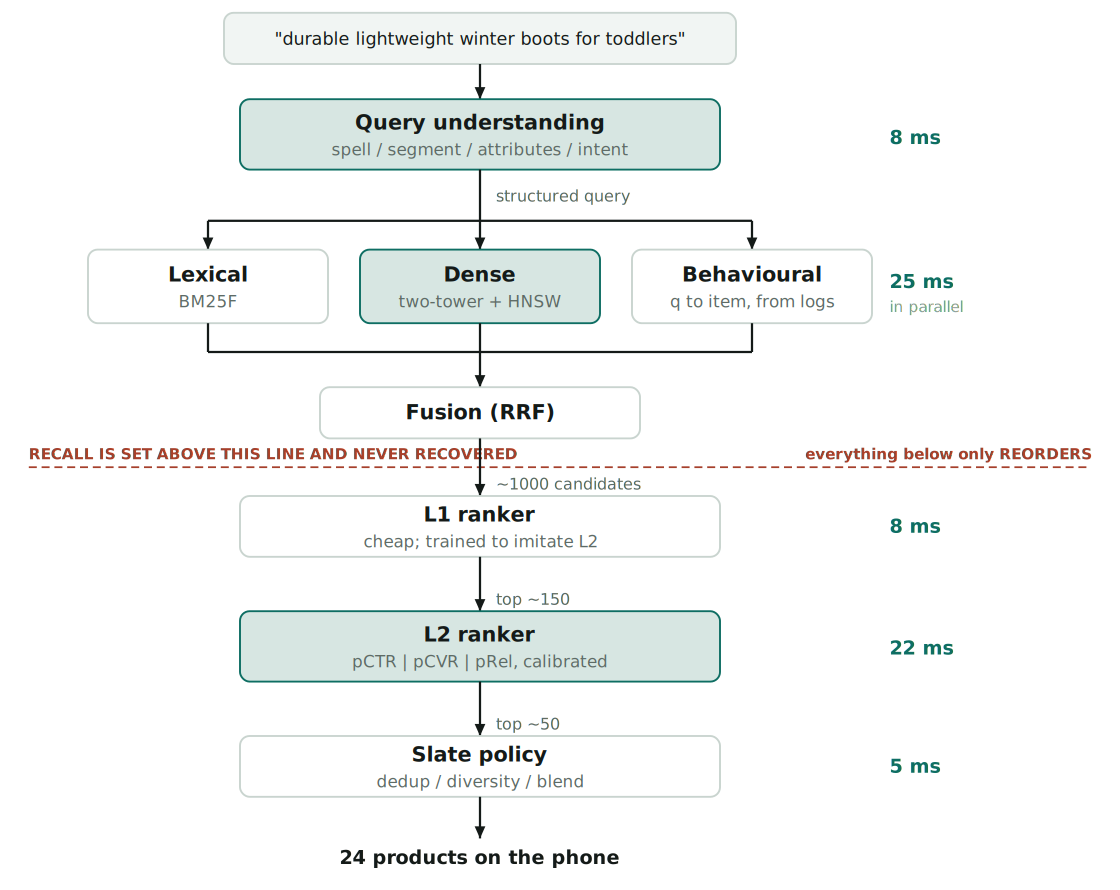
\includegraphics[width=\linewidth]{figures/funnel.pdf}\par\vspace{3pt}
\nopagebreak{\footnotesize\color{muted}Figure 1. The funnel. Each stage sees roughly ten times fewer items and costs ten times more per item, which is why every stage takes about the same wall-clock.\par}\medskip
\begin{decide}{How many retrieval arms?}
\drow{CHOSE}{Lexical + dense + behavioural, fused}
\drow{OVER}{Dense only, which is what the prompt's wording tempts you into}
\drow{WHY}{they fail on disjoint query populations. Dense dies on part numbers and rare identifiers; lexical dies on the paraphrase in the prompt; behavioural is empty on the tail and unbeatable on the head.}
\drow{COST}{three indexes to keep in sync, and a fusion layer that has to be learned rather than constant}
\drow{DROP IT IF}{the dense arm's unique contribution -- clicked items only it retrieved -- turns out to be small. Measure, do not assume.}
\end{decide}
Three things to say while you draw it.\par
\textbf{The three retrieval arms exist because they fail on disjoint query populations.} Lexical nails exact tokens and part numbers and dies on paraphrase. Dense nails paraphrase and intent and dies on rare identifiers. Behavioural --- a query-to-item table mined from six months of logs --- beats both on head queries and has nothing at all for the tail. The tail query in the prompt is precisely the case where only the dense arm helps, which is why the question is worded the way it is.\par
\textbf{Recall is set here and can never be recovered.} Everything downstream only reorders. So retrieval gets measured on recall, ranking on order, and confusing the two produces months of wasted experiments.\par
\textbf{L1 exists to protect L2's budget.} A cheap model over 1000 candidates lets the expensive model see 150. Without it you either score 1000 with something cheap, or blow the budget.\par
\csection{The latency budget, and three ways to spend it}
I am assuming 100 ms is end-to-end server-side p99, which is the harder reading. Fan-out costs are real and candidates routinely forget them: serialisation, merge, and network between services will eat 15--25 ms before any model runs.\par
\textbf{Option A --- all-CPU, no cross-encoder.}\par
\par\vspace{6pt}\noindent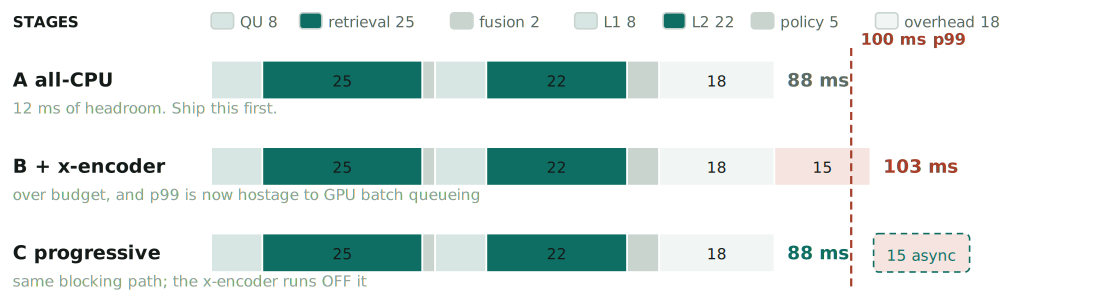
\includegraphics[width=\linewidth]{figures/latency.pdf}\par\vspace{3pt}
\nopagebreak{\footnotesize\color{muted}Figure 2. Three ways to spend 100 ms. A already leaves only 12 ms of headroom, which is why the cross-encoder does not fit in the blocking path at all.\par}\medskip
Twelve milliseconds of headroom, and everything runs on commodity CPU. This is what I would ship first.\par
\textbf{Option B --- put a cross-encoder reranker over the top 50.} A 6-layer MiniLM-class model at 128 tokens, batch 50, runs in roughly 10--15 ms on a T4-class GPU. That is \textasciitilde{}103 ms and it is over budget before you have accounted for anything going wrong. And the way it goes wrong is specific: under load, GPU batch formation and admission control dominate, and the tail of a GPU service is far worse behaved than its median --- so the number you actually measure at p99 will be worse than 103.\par
\textbf{Option C --- progressive ranking, which is the answer I would defend.}\par
The tempting move is to make the expensive path rare: route tail queries through the cross-encoder and head queries around it. \textbf{That does not work, and knowing why is the point.} p99 \textit{is} the tail. If 30\% of queries take 103 ms, then p99 is 103 ms --- making the expensive path rare only helps if ``rare'' means under one percent, and by then it is not doing enough work to matter.\par
The same reasoning kills the other reflex. \textbf{Caching the head does not help your p99 either}, for exactly the same reason: the cached queries are the fast ones, and p99 is measured on the slow ones. A query cache is a cost and median-latency win, not an SLO win, and saying so unprompted is a small but real signal.\par
What does work is taking the expensive model off the blocking path. On a mobile grid the first screen is four to six items. Serve those from the cheap path inside budget, then run the cross-encoder over the remaining candidates during the user's dwell time and deliver the reordered result with the next scroll page. The blocking p99 stays at 88 ms; the cross-encoder still improves the session. It costs you a more complicated client contract and a reordering that must be stable enough not to feel like the page is shuffling under the user.\par
There is still a role for adaptive depth, but on the retrieval side rather than the ranking side: give tail queries a larger \texttt{ef\_search} and deeper candidate sets, since that cost sits inside the parallel arms where there is slack.\par
One policy to state without being asked: \textbf{never degrade by silently dropping a retrieval arm on timeout.} That converts a latency problem into an invisible quality problem that shows up weeks later as an unattributable relevance regression. Degrade by reducing depth --- lower \texttt{ef\_search}, fewer L2 candidates --- and emit a metric every time you do, so the degradation is measurable.\par
\cchapter{Query understanding on the tail}
Take the query in the prompt apart on the board, because it demonstrates the problem better than any description of it.\par
\par\noindent{\small\setlength{\tabcolsep}{4pt}%
\begin{tabularx}{\linewidth}{YYY}\hline
\textbf{Token} & \textbf{What it is} & \textbf{Binds to} \\ \hline
durable & quality attribute, soft & no catalogue field at all \\
lightweight & physical attribute & sometimes in specs, usually only in free text \\
winter & season / use-case & insulation, waterproofing \\
\textbf{boots} & \textbf{head noun} & \textbf{category --- the one hard constraint} \\
for toddlers & audience & age 1--3, so a size band --- a real filter \\
\hline\end{tabularx}}\par\medskip
\textbf{Hard constraints:} category = boots, audience = toddler. \textbf{Soft preferences:} durable, lightweight, winter-appropriate. \textbf{What BM25 sees:} six tokens, each appearing in thousands of listings and almost never co-occurring.\par
\begin{callouttrap}Read the example query back to her before you answer. ``Durable lightweight winter boots for toddlers'' is not decoration -- it was chosen so that lexical retrieval fails, and demonstrating that you noticed is worth more than any architecture you propose in the next five minutes.\end{callouttrap}
Now the point: \textbf{BM25 will return either nothing or garbage here.} Require all six terms and you get near-zero results because no title contains them all. Relax to OR-with-coordination and the scoring is dominated by whichever term is rarest --- probably ``toddlers'' --- so you retrieve toddler clothing rather than boots. This is the classic tail failure, and it is why the dense arm is not optional.\par
What I would build:\par
\textbf{Head-noun and category prediction, with a confidence gate.} Getting \texttt{category = boots} right is worth more than everything else in query understanding combined. Predict it, and apply it as a retrieval filter \textit{only} above a high confidence threshold, with a fallback pass that re-runs unfiltered if the filtered pass returns too few. Below threshold it goes in as a ranking feature. The asymmetry matters: a wrong filter deletes results with no recovery, a wrong feature just gets outvoted.\par
\textbf{Attribute extraction as sequence labelling}, trained on catalogue structured data rather than hand annotation. You already know each product's category, audience, colour, size. Reverse that into weak labels over the query side by mining queries that led to purchases of products with a given attribute. Six months of logs is exactly what this needs.\par
\textbf{Precompute the head, model the tail.} The top few thousand queries carry a large share of sessions. Precompute their entire understanding offline, review them, and serve from a lookup. That gives you editorial control where the traffic is, costs nothing at serving time, and leaves the live model path for the tail --- which is also where you can afford deeper retrieval, per Option C.\par
\textbf{Where an LLM belongs here.} Offline, generating attribute annotations and query rewrites for the tail, distilled into a small model or baked into a table. Not in the 8 ms online path. Say this unprompted; it is a question she will otherwise ask.\par
\cchapter{Retrieval: half the answer}
\csection{The architecture, and the asymmetry that defines it}
\par\vspace{6pt}\noindent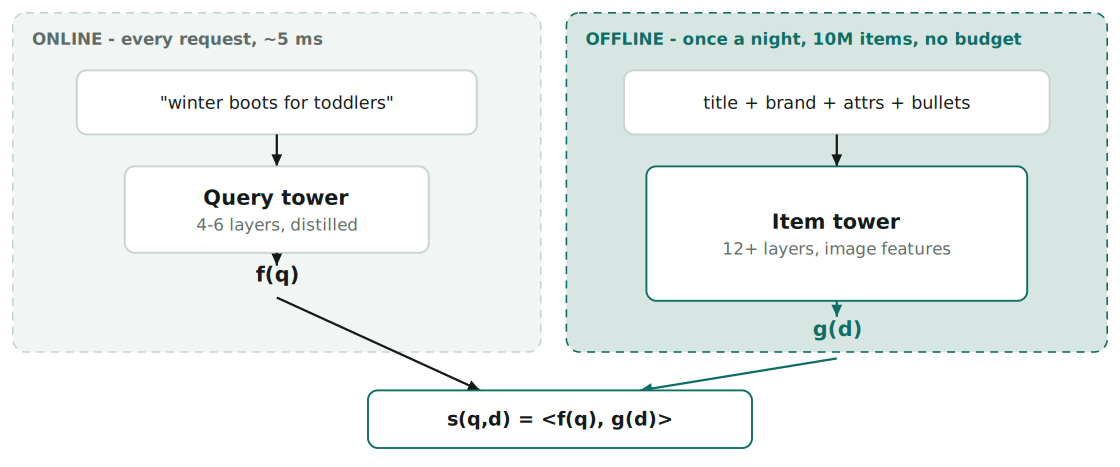
\includegraphics[width=\linewidth]{figures/two-tower.pdf}\par\vspace{3pt}
\nopagebreak{\footnotesize\color{muted}Figure 4. The two towers are deliberately different sizes. The item tower can be large precisely because nobody is waiting for it -- that is free capacity most candidates leave on the table by drawing two identical boxes.\par}\medskip
State the asymmetry explicitly, because most candidates draw two identical boxes. \textbf{The item tower runs offline over 10M products once a night; the query tower runs inside your latency budget on every request.} So you can afford a large item encoder and you cannot afford a large query encoder. That is free capacity most people leave on the table --- and it is the reason two-tower beats a single shared encoder in production even though sharing weights looks tidier.\par
The other consequence of the architecture: query and item never interact before the dot product. That is what makes ANN possible, and it is also the ceiling on quality. No amount of training makes a two-tower model reason about the interaction between ``lightweight'' and a particular boot's spec sheet the way a cross-encoder can. So the two-tower's job is recall, and you accept that.\par
\csection{Where the positives come from}
Six months of logs, and the choice of positive is a modelling decision, not a data-loading detail. Three questions in order: which actions count, how much each is worth, and what the resulting table looks like.\par
\csubsection{The action ladder}
\par\noindent{\small\setlength{\tabcolsep}{4pt}%
\begin{tabularx}{\linewidth}{YYYYY}\hline
\textbf{Action} & \textbf{Count, 6 months} & \textbf{Rate} & \textbf{What it is evidence of} & \textbf{Value $v(a)$} \\ \hline
Impression & \textasciitilde{}62B & \textasciitilde{}20 / search & the ranker's opinion, not the user's & baseline, 0 \\
Click & \textasciitilde{}1.2B & 0.4 / search & interest \textbf{given the thumbnail and price} & 1.0 \\
Add to cart & \textasciitilde{}180M & 0.06 / search & genuine consideration & 1.9 \\
Purchase & \textasciitilde{}60M & 0.02 / search & intent satisfied & 2.6 \\
Purchase, returned & \textasciitilde{}6M & 10\% of purchases & relevant, but did not fit & 1.6 \\
\hline\end{tabularx}}\par\medskip
The naive choice is clicks, because there are 1.2 billion of them. The problem is that a click in commerce is driven by the thumbnail and the price as much as by relevance, so a click-trained retriever learns attractiveness. The naive correction is to train on purchases only --- but 60M events spread across 10M products is far too sparse for the tail, and the tail is the question.\par
So: \textbf{train on clicks for coverage, and weight by the downstream action.}\par
\csubsection{How the values are derived, not chosen}
This is the part worth being precise about, because ``a purchase is worth more'' is not an answer --- \textit{how much} more is the answer, and picking it by taste is how you end up with a model nobody can debug.\par
The weight should be monotone in \textbf{the posterior probability that this item is genuinely relevant to this query, given that this action happened.} That is measurable. Take a few thousand query-item pairs, stratified by which action they received, have humans judge relevance, and compute $P(\text{rel} \mid a)$ per action. Then set the value to the log-odds, with impression as the baseline:\par
\begin{mathbox}\[v(a) \;=\; \mathrm{logit}\,P(\text{rel} \mid a) \;-\; \mathrm{logit}\,P(\text{rel} \mid \text{impression})\]\end{mathbox}
normalised so a click is 1.0. A few thousand judgements is a day of annotation and it converts every weight in the pipeline from an opinion into a measurement.\par
\begin{callouttrap}The calibrated values come out far flatter than intuition. Most people reach for a purchase being ten times a click; the likelihood ratio says about two and a half. The click already carries most of the relevance evidence --- the purchase adds price, availability and delivery, which are ranking concerns, not retrieval ones. Say this out loud; it is the kind of thing that only comes from having measured it.\end{callouttrap}
The returns row carries the same lesson and is worth volunteering. A returned purchase is \textbf{still good evidence of relevance} --- the customer searched, found it, and bought it. The return usually means fit or quality, not the wrong product. So returns barely move the retriever and matter enormously to the ranker.\par
\begin{calloutsay}Returns are a ranking signal, not a retrieval signal. The item was relevant; it just did not fit. I would penalise them heavily in the expected-value objective and almost not at all in the retriever's positives.\end{calloutsay}
\csubsection{Scoring one pair}
\par\vspace{6pt}\noindent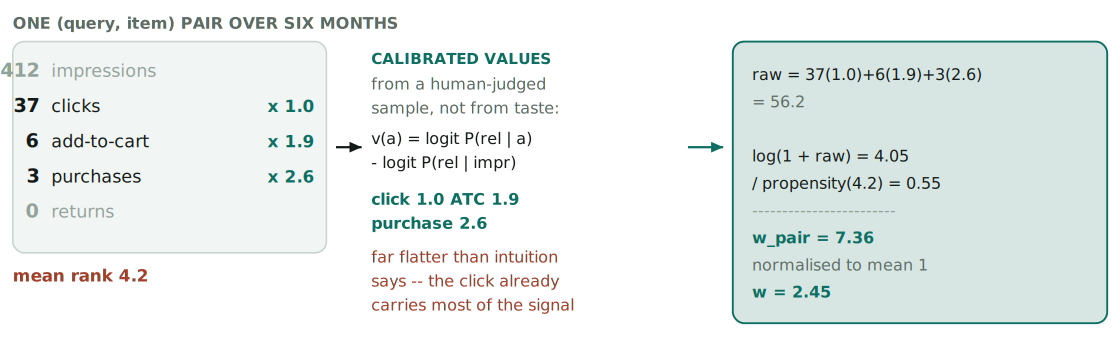
\includegraphics[width=\linewidth]{figures/positives.pdf}\par\vspace{3pt}
\nopagebreak{\footnotesize\color{muted}Figure 4b. The weight for one (query, item) positive. Counts times calibrated values, log-compressed so a pair with ten thousand clicks does not get ten thousand times the weight of one with a single click, then divided by examination propensity, then normalised so the dataset mean is 1.\par}\medskip
\begin{mathbox}\[w(q,d) \;=\; \frac{\log\!\big(1 + \sum_a n_a(q,d)\, v(a)\big)}{\hat{\pi}\big(\overline{\text{rank}}, \text{surface}\big)}\]\end{mathbox}
Three choices inside that formula, each of which she can push on.\par
\textbf{The log.} Without it, a pair with 10,000 clicks contributes 10,000 times the gradient of a pair with one, and your retriever becomes a popularity model. The log is the same saturation intuition as BM25's $k_1$, applied to training weight instead of term frequency.\par
\textbf{The propensity divisor.} A click at rank 1 is weak evidence because rank 1 is examined regardless; a click at rank 20 is strong evidence because the user had to work for it. Dividing by $\hat{\pi}$ up-weights the deep clicks. \textbf{Clip it} --- $\hat{\pi} \geq 0.05$ or so --- because a propensity estimate near zero produces a weight that dominates the entire batch.\par
\textbf{The normalisation.} Scale weights to mean 1 across the dataset so the loss magnitude, and therefore your learning rate, does not move when you change the value table.\par
\csubsection{Where the weight actually goes}
Two mechanically different options, and the choice matters more than it looks.\par
\begin{decide}{How do you apply the positive weight?}
\drow{CHOSE}{Sample positives with probability proportional to $w$, capped, and then train unweighted}
\drow{OVER}{Keeping the batch uniform and multiplying each example's loss term by $w$}
\drow{WHY}{with in-batch negatives every positive is simultaneously a negative for the other queries in the batch. Loss-weighting only scales its role as a positive, so a heavily weighted pair is a loud positive and a normal-volume negative -- an asymmetry nobody intends. Sampling changes both roles consistently.}
\drow{COST}{sampling amplifies popularity, so the log compression and the cap are load-bearing, and you lose the ability to tune weights without rebuilding the sampler}
\drow{FALLBACK}{sample for the bulk of the signal and loss-weight only the returns adjustment, which is small}
\end{decide}
\csubsection{Session-level attribution for the tail}
For a tail query with a handful of events, a single click is noise. But reformulation chains are signal, and this is the cheapest tail data you have.\par
The rule I would write down, because ``attribute the session'' is not specific enough to implement:\par
\begin{itemize}
\item A session is one user, events within a 30-minute gap.
\item If query $q_1$ produced no click, the user reformulated to $q_2$, and then clicked or purchased item $d$ --- attribute $d$ as a positive for \textbf{both} $q_1$ and $q_2$.
\item Discount the inferred one: $q_1$ gets $0.5 \times w$, because the attribution is an inference and $q_2$ is the observation.
\item Cap the chain at two reformulations. Beyond that the user has changed intent.
\item Require the two queries to share a token or exceed a similarity threshold, or you will attribute ``toddler boots'' to ``phone charger'' in the same session.
\end{itemize}
On this corpus that typically recovers training pairs for a meaningful slice of tail queries that otherwise have no positive at all --- which is exactly the population the prompt is about.\par
\csection{The shape of the training data}
Two tables, and \textbf{they are different shapes on purpose}.\par
\csubsection{The event log --- what you read from}
\begin{Verbatim}[fontsize=\small,xleftmargin=4pt,samepage=false]
search_event      search_id, user_id, ts, query_raw, query_norm,
                  surface, locale, ranker_version, retriever_version
impression_event  search_id, item_id, position(row,col), above_fold, ts
action_event      search_id, item_id, action, ts, order_id
\end{Verbatim}
\texttt{ranker\_version} and \texttt{retriever\_version} are not bookkeeping --- they are what makes intervention harvesting possible later, because they identify the natural position randomisation your A/B tests already produced.\par
\csubsection{The retriever's table --- aggregated to the pair}
\begin{Verbatim}[fontsize=\small,xleftmargin=4pt,samepage=false]
retriever_pairs                                        ~180M rows
  query_norm          string
  item_id             int64
  n_impr, n_click, n_atc, n_purchase, n_return   int
  mean_position       float
  propensity          float        -- clipped
  weight              float        -- the formula above, normalised
  query_freq_bucket   enum(head, torso, tail)
  split               enum(train, val, test)
\end{Verbatim}
\textbf{Why aggregate.} The retriever has no user features --- the query tower sees a string and nothing else --- so per-event rows add no information, and they add popularity skew: a pair shown a million times would contribute a million gradient steps for a signal that is fully captured by its counts. Aggregating deduplicates it and costs nothing.\par
Filters worth naming: drop pairs with zero clicks, drop queries with fewer than three distinct clicked items (no contrast to learn from), drop bot and scraper traffic by session-rate heuristics, and drop pairs whose item is no longer in the catalogue.\par
\csubsection{The ranker's table --- per impression}
\begin{Verbatim}[fontsize=\footnotesize,xleftmargin=4pt,samepage=false]
ranker_impressions                                     ~62B, sampled to ~2B
  search_id, item_id, position, surface, device, ts
  feature_vector      float32[~200]   -- LOGGED at serve time, not recomputed
  label_click, label_atc, label_purchase, label_return  bool
  propensity          float
  split               enum
\end{Verbatim}
The ranker \textit{does} have user and context features, so it needs per-impression rows, and it needs the negatives that never got clicked --- which the retriever's table has thrown away. The \texttt{feature\_vector} is logged rather than recomputed, for the skew reason in Figure 13.\par
\begin{calloutsay}The two tables are different shapes because the retriever has no user context. That is not an implementation detail --- it is why the retriever can be trained on an aggregate a thousand times smaller than the ranker's.\end{calloutsay}
\csubsection{The batch that comes out}
\par\noindent{\small\setlength{\tabcolsep}{4pt}%
\begin{tabularx}{\linewidth}{YYY}\hline
\textbf{Tensor} & \textbf{Shape} & \textbf{Notes} \\ \hline
\texttt{query\_ids} & \texttt{[4096, 16]} & queries are short; 16 tokens covers almost all \\
\texttt{pos\_item\_ids} & \texttt{[4096, 96]} & title + brand + attributes \\
\texttt{hard\_neg\_ids} & \texttt{[4096, 4, 96]} & 2 from BM25, 2 from the current ANN index \\
\texttt{uni\_neg\_ids} & \texttt{[4096, 2, 96]} & uniform over the 10M index \\
\texttt{weights} & \texttt{[4096]} & only if you loss-weight rather than sample \\
\texttt{log\_q} & \texttt{[4096, 4102]} & sampling log-prob per candidate, for the logQ correction \\
\hline\end{tabularx}}\par\medskip
Candidates per query: 1 positive + 4095 in-batch + 4 mined + 2 uniform $\approx$ \textbf{4102}.\par
\begin{calloutnum}Item-tower forward passes per step: 4096 positives + 4096 x 6 explicit negatives = 28,672. In-batch negatives are free; every mined or uniform negative is a full encoder pass. That factor of seven is the real cost of the negative strategy, and it is the number to quote if she asks what it costs.\end{calloutnum}
The mitigation, which is what ANCE does in practice: cache item embeddings from the last index refresh and reuse them for mined negatives, recomputing only on the refresh cadence. You trade a little staleness for most of the compute.\par
\csubsection{The negative sources, side by side}
\par\noindent{\small\setlength{\tabcolsep}{4pt}%
\begin{tabularx}{\linewidth}{YYYYY}\hline
\textbf{Source} & \textbf{Per positive} & \textbf{Cost per step} & \textbf{What it fixes} & \textbf{Fails if} \\ \hline
\textbf{In-batch} & \textasciitilde{}4095 & free --- already encoded & general contrast, cheaply & used alone: popularity-biased, cannot reach the tail \\
\textbf{Mined, BM25} & 2 & 2 encoder passes & keyword match vs intent match & not filtered --- BM25's top-k is full of false negatives \\
\textbf{Mined, ANN} & 2 & 2 passes + re-index & the model's \textit{current} errors & not refreshed --- they go stale once the model beats the miner \\
\textbf{Uniform} & 2 & 2 passes & the zero-engagement tail & nothing: they are cheap and they are the only source that covers it \\
\hline\end{tabularx}}\par\medskip
\csubsection{Splits}
\textbf{Split by time, never randomly.} The last 14 days are test, the 14 before are validation, everything earlier is train. A random split leaks: the same (query, item) pair appears on both sides, and you will serve forward in time, so a random split measures a task you will never perform.\par
Hold out a second, \textbf{query-disjoint} split as well --- whole tail queries the model has never seen --- because time-based splitting still lets a head query's embedding be learned from the training period and evaluated in the test period. That second split is the one that tells you about the tail.\par
\csection{The objective}
Retrieval is trained as a classification problem over the corpus: given the query, pick the right item out of everything. The full softmax over 10M items is intractable, so you sample.\par
\begin{mathbox}\[\mathcal{L} \;=\; -\log
\frac{\exp\!\big(s(q,d^{+})/\tau\big)}
     {\sum_{d \in \{d^{+}\}\cup N} \exp\!\big(s(q,d)/\tau\big)}\]\end{mathbox}
where $s(q,d)=\langle f(q), g(d)\rangle$, $\tau$ is the temperature, and $N$ is the sampled negative set for this query. It is a cross-entropy over a sampled candidate set: push the positive up, push everything else down, with $\tau$ setting how sharply.\par
\csection{Which loss, and why not the others}
This is worth being properly fluent on, because ``contrastive learning \ldots{} or softmax'' is two thirds of what her scorecard named. The families differ in one thing that explains everything else: \textbf{what a single gradient step is allowed to see.}\par
\par\vspace{6pt}\noindent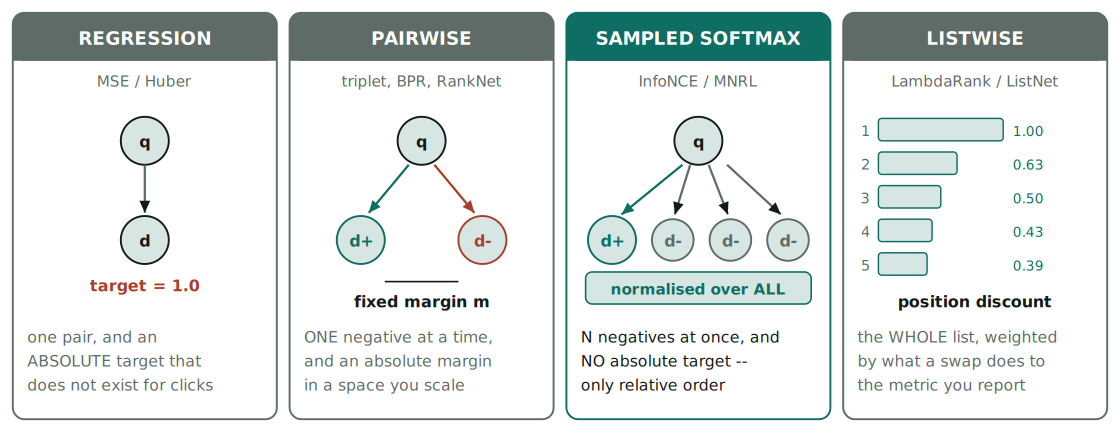
\includegraphics[width=\linewidth]{figures/losses.pdf}\par\vspace{3pt}
\nopagebreak{\footnotesize\color{muted}Figure 5b. One gradient step, four ways. Regression needs an absolute target that click data does not provide. Pairwise sees one negative and a margin measured in a space whose scale the model controls. Sampled softmax sees many negatives and has no absolute target at all --- only relative order. Listwise sees the whole list and weights each swap by what it does to the metric.\par}\medskip
\csubsection{The one-question rule}
Ask what the output is \textbf{consumed as}, and the loss follows:\par
\par\noindent{\small\setlength{\tabcolsep}{4pt}%
\begin{tabularx}{\linewidth}{YYY}\hline
\textbf{The output is consumed as} & \textbf{Use} & \textbf{Because} \\ \hline
An ordering over millions of items & \textbf{Sampled softmax / InfoNCE} & only relative order matters, and normalising over sampled negatives is the cheapest unbiased way to get it \\
An ordering over a short list where position matters & \textbf{Listwise, metric-weighted} (LambdaRank) & you can afford to look at the whole list, and NDCG's discount should drive the gradient \\
A probability you will multiply or threshold & \textbf{Pointwise BCE}, then calibrate & the expected-value product is meaningless unless the number is a probability \\
A yes/no decision at a threshold & \textbf{Contrastive pair / triplet} & you need an absolute decision boundary in the metric, not a ranking \\
A number with units & \textbf{Regression} (Huber over MSE, for outliers) & there is a real target and its magnitude is the answer \\
A teacher's ordering & \textbf{Margin-MSE or KL} & the ordering is the signal; the teacher's absolute scale is not \\
\hline\end{tabularx}}\par\medskip
\csubsection{Why not MSE}
Three reasons, and the first one ends the conversation.\par
\textbf{There is no target.} A click is not a similarity of 1.0. To use MSE you would have to invent the label, and whatever you invented would be the thing the model learned. Retrieval supervision is ordinal by nature: this item beat that one for this query. MSE requires cardinal supervision you do not have.\par
\textbf{It optimises the wrong quantity.} Even granting a target, retrieval only ever uses the \textit{order} of the scores. MSE spends capacity matching magnitudes that are never read, and the capacity comes out of the ordering you do care about.\par
\textbf{Nothing forces the positive to win.} MSE has no normalisation across candidates. A model that outputs 0.3 for every pair has a respectable MSE against a mostly-negative dataset and precisely zero retrieval utility. The softmax's denominator is the entire point: the positive can only score well by \textit{beating the others}.\par
There is a fourth, quieter one: the gradient is dominated by the easy mass. Almost every query-item pair in a 10M catalogue is trivially unrelated and already predicted near zero, so most of the MSE gradient is spent confirming things the model already knows.\par
\csubsection{Why not triplet, and when it is actually right}
Triplet is not a silly choice --- it is the previous generation's answer, and it still wins in one setting. But for retrieval the softmax dominates it on four axes.\par
\textbf{One negative per step.} Triplet's gradient says ``be further from this one thing.'' The softmax's says ``beat all of these at once,'' which is a far lower variance estimate of the objective you actually serve.\par
\textbf{The margin is absolute in a space you control.} With unnormalised embeddings the model can satisfy any margin by inflating norms and learning nothing about the geometry. That is why triplet effectively forces L2 normalisation --- and once you are on the unit sphere, distances live in a fixed narrow range and the margin becomes a very tight budget to tune. The softmax's temperature does the same job \textit{relatively}, so it is scale-free.\par
\textbf{The hinge switches off.} Once a triplet satisfies the margin, its loss is exactly zero and it contributes no gradient. Late in training most of the batch contributes nothing, which is why semi-hard mining exists and why it is fiddly. The softmax is smooth: every negative always contributes something, weighted by how close it came.\par
\textbf{Collapse.} With easy negatives, triplet can drive everything to a point and report a happy loss curve. The normalisation makes that much harder to achieve under a softmax.\par
\begin{calloutpush}``So triplet is just worse?'' --- No. Triplet and contrastive-pair losses give you a \textit{calibrated distance} with a decision boundary; softmax gives you an ordering with no absolute meaning. If the product needs ``are these two things the same?'' as a yes/no at a threshold, you want the margin. That is verification, not retrieval.\end{calloutpush}
And that case exists in this very system. \textbf{Catalogue deduplication} --- deciding whether two seller listings are the same physical product, which a marketplace has to do constantly and which feeds the slate policy's dedup step --- is a verification problem with a threshold. I would train that with a contrastive pair loss, not a softmax, and I would say so if she asks whether contrastive losses have any place here.\par
\csubsection{Where MSE is actually the right answer}
Two places, both inside this design, and naming them is the cleanest way to show you are not just reciting ``softmax good, MSE bad.''\par
\textbf{Distilling the cross-encoder into the bi-encoder.} The teacher produces real scores, so regression is available. But regress the \textbf{margin}, not the raw score --- $s(q,d^{+}) - s(q,d^{-})$ for the student matched to the same difference for the teacher. The teacher's absolute scale is arbitrary, so fitting it forces the student to waste capacity on an offset that means nothing; the margin is what carries the ordering, and it is invariant to that scale. That is Margin-MSE, and it is the reason plain MSE distillation underperforms.\par
The alternative is KL over the softmax of the candidate set, which transfers the whole distribution rather than pairwise gaps. Margin-MSE is simpler and robust; KL carries more information when your candidate sets are consistent. I would start with Margin-MSE.\par
\textbf{Training L1 to imitate L2.} L1's job is to not discard anything L2 would have wanted, so it is a distillation problem, and regression onto L2's scores is a reasonable objective --- with the same caveat, that a ranking-aware distillation beats plain MSE because only the top-k ordering matters.\par
\csubsection{The whole system, loss by loss}
If she asks you to put it together --- and this is a good thing to volunteer --- every trained component in the design has a different loss, for a reason:\par
\par\noindent{\small\setlength{\tabcolsep}{4pt}%
\begin{tabularx}{\linewidth}{YYY}\hline
\textbf{Component} & \textbf{Loss} & \textbf{Why that one} \\ \hline
Two-tower retriever & Sampled softmax + logQ correction & ordering over 10M, no calibration needed downstream \\
Cross-encoder teacher & Listwise CE on graded labels & short candidate sets, graded judgements available \\
Bi-encoder distillation & Margin-MSE, or KL over candidates & transfers ordering, invariant to teacher scale \\
L1 ranker & Ranking distillation from L2 & measured on recall of L2's top-k, not NDCG \\
pCTR, pCVR, pReturn & BCE, then post-hoc calibration & they get multiplied by price \\
pRel gate & Listwise, or distilled from the cross-encoder & a gate, not a probability \\
Slate re-ranking layer & Listwise over the final top-k & list context is the whole point \\
Catalogue dedup & Contrastive pair with a margin & verification at a threshold \\
Delivery-time feature & Huber regression & a real number with units, and outliers \\
\hline\end{tabularx}}\par\medskip
\begin{decide}{Which loss for the retriever?}
\drow{CHOSE}{Sampled softmax / InfoNCE over the sampled candidate set, with the logQ correction}
\drow{OVER}{Triplet with a margin, BPR/RankNet, and MSE regression}
\drow{WHY}{retrieval consumes only the ordering, and the softmax is the only one of these that normalises over many candidates at once --- so the gradient estimates ``beat everything'' rather than ``beat this one thing'', and it needs no absolute target, which click data cannot provide anyway}
\drow{COST}{large batches to get enough negatives, a temperature to tune, and an output with no probabilistic meaning}
\drow{BUT}{keep a contrastive pair loss for catalogue dedup, which is verification at a threshold rather than ranking, and Margin-MSE for distilling the cross-encoder}
\end{decide}
Three things follow.\par
\textbf{The number of negatives is the difficulty knob.} More negatives means a harder classification task and a better-conditioned gradient, which is why these models train at batch sizes in the thousands with cross-device negative sharing.\par
\textbf{Temperature matters more than people expect.} With L2-normalised embeddings the score lives in [-1, 1], so without a small temperature the softmax is nearly uniform and there is almost no gradient. Typical values are 0.01--0.05. Push it too low and the gradient concentrates entirely on the single hardest negative, which is unstable and can collapse the representation. It can be learned --- CLIP learns log-temperature with a clamp --- and I would start at 0.05, tune it, and watch the positive-score distribution rather than only the loss.\par
\csection{Negatives: where this model is actually won or lost}
This is the sub-topic to be deepest on. It is named in the scorecard and it is where a candidate with real experience separates from one who has read papers.\par
\csubsection{In-batch negatives, and the bias they introduce}
In a batch of N pairs, use the other N-1 items as negatives for each query. Free --- no extra forward passes, since you already encoded them.\par
The catch: \textbf{your batch is not a uniform sample of the corpus.} It is sampled from the click stream, so an item appears as a negative in proportion to how often it is clicked. Popular items are therefore pushed down constantly, and the model learns to under-score exactly the items that convert best. In commerce that is precisely backwards.\par
The fix is the \textbf{logQ correction}, also called sampling-bias correction:\par
\begin{mathbox}\[s'(q,d) \;=\; s(q,d) \;-\; \log p(d)\]\end{mathbox}
$p(d)$ is the probability that item $d$ is drawn as a sampled negative, which is essentially its frequency in the training stream. Estimate it online with a streaming counter: track the average gap in steps between consecutive occurrences of $d$, and take $p(d)\approx 1/\text{gap}$.\par
The intuition to say out loud: an item that shows up as a negative ten times as often should be penalised a tenth as hard each time. Without it, the retriever has a systematic anti-popularity bias. This is the correction from the YouTube two-tower work, and naming it is worth doing.\par
\par\vspace{6pt}\noindent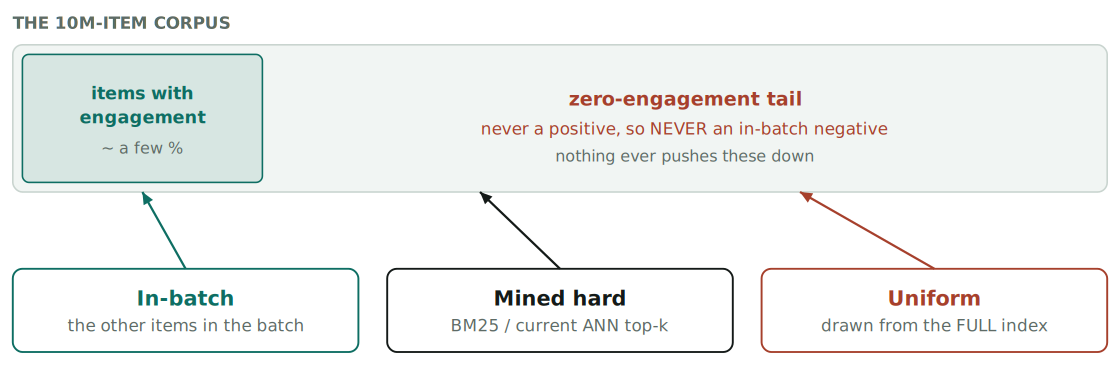
\includegraphics[width=\linewidth]{figures/negatives.pdf}\par\vspace{3pt}
\nopagebreak{\footnotesize\color{muted}Figure 6b. Where each negative source can reach. In-batch negatives are drawn from the click stream, so they can only ever be items that appear as a positive somewhere in the batch. At 10M products with a long tail, that leaves most of the corpus untouched.\par}\medskip
\csubsection{The negatives that are never sampled at all}
Here is the part most candidates miss, and it matters enormously at 10M products. \textbf{In-batch negatives can only ever be items that appear as a positive somewhere in the batch} --- that is, items with engagement. In a 10M-product catalogue with a long tail, a large fraction of items have essentially zero clicks in six months. Those items are never negatives for anyone. The model has therefore never been trained to push them down, their embeddings sit wherever initialisation and the item-text encoder put them, and they can surface spuriously in ANN results for unrelated queries.\par
\begin{decide}{Where do negatives come from?}
\drow{CHOSE}{In-batch with the logQ correction, plus mined hard negatives refreshed from the current model, plus uniform draws from the full index}
\drow{OVER}{In-batch only, which is the default in every tutorial}
\drow{WHY}{in-batch alone is biased toward popular items and structurally cannot reach the zero-engagement tail; hard negatives teach the distinctions that matter; uniform draws are the only source that covers the whole corpus}
\drow{COST}{a mining pipeline, a cross-encoder to filter false negatives, and a ratio to tune}
\end{decide}
The fix is \textbf{mixed negative sampling}: in-batch negatives plus a set of negatives drawn uniformly from the full item index. The uniform ones are easy and contribute little gradient individually, but they are the only thing covering the zero-engagement tail, and they are cheap.\par
\csubsection{Hard negatives}
Random and in-batch negatives are mostly trivially wrong --- a laptop for a boots query. The model saturates on them quickly and stops learning the distinctions that matter. Hard negatives are items that look right and are not: toddler \textit{shoes} for a toddler \textit{boots} query; adult winter boots; boots that are neither lightweight nor durable.\par
Two sources, in order of sophistication:\par
\begin{itemize}
\item \textbf{BM25 top-k, not clicked.} Cheap, no model needed, and a good first pass.
\item \textbf{The model's own ANN top-k, refreshed periodically} --- this is ANCE. As the model improves, yesterday's hard negatives stop being hard, so you re-mine from the current index every epoch or two. Static hard negatives go stale and you silently stop learning from them.
\end{itemize}
A typical recipe: one positive, a handful of mined hard negatives, the whole batch as in-batch negatives, plus uniform negatives. The ratio is worth tuning; all-hard is a known failure mode.\par
\csubsection{False negatives, and why they are worse than no negatives}
A mined ``hard negative'' is often just an unclicked relevant item --- the user bought one pair of boots, not all five good ones. Training on it teaches the model that a correct answer is wrong, which is actively destructive rather than merely unhelpful.\par
\textbf{Denoise with a cross-encoder.} Score every mined negative with a cross-encoder teacher and drop any that scores above the positive, or above a threshold. This is the RocketQA recipe and it is usually worth more than any architecture change you could make instead. If she asks what to do without a cross-encoder: drop mined negatives that were clicked by anyone for a similar query, and drop those whose category matches the query's predicted category exactly.\par
\csection{Distillation: the highest-leverage step people skip}
Train a cross-encoder on the same data. It is far more accurate because query and item interact. Then use it as a teacher: score a large set of query-item pairs and train the bi-encoder to match the teacher's \textit{score distribution} rather than the binary click label --- KL on the softmax over the candidate set, or a margin-MSE on score differences.\par
Why this is worth saying: the binary label carries one bit. The teacher's scores carry the full ordering, including how much better the positive is than each negative. That ordering information is exactly what a retriever needs and what clicks cannot provide. In my experience this buys more than doubling the embedding dimension or adding layers.\par
And it closes the loop nicely: you need the cross-encoder anyway for false-negative filtering and for the progressive reranker, so you get three uses out of training it once.\par
\csection{Embedding geometry}
Three decisions, each with a specific consequence.\par
\textbf{Normalise or not.} L2-normalise both towers and use cosine, and every item lives on the unit sphere so magnitude cannot encode popularity. That is what you want for a relevance retriever; popularity belongs in the ranker where it can be traded off explicitly. Leaving embeddings unnormalised lets magnitude carry a quality prior, which helps in pure recsys retrieval and hurts here.\par
\begin{decide}{Normalise the embeddings?}
\drow{CHOSE}{L2-normalise both towers, cosine similarity, temperature in the loss}
\drow{OVER}{Unnormalised dot product, where magnitude carries a popularity prior}
\drow{WHY}{popularity belongs in the ranker where it can be traded off explicitly, not smuggled into the retrieval score where you cannot see it}
\drow{COST}{you need the temperature, since cosine lives in [-1, 1] and the softmax is otherwise nearly flat}
\end{decide}
\textbf{Whatever you choose, serve it the same way.} Training with unnormalised dot product and then serving a cosine index silently discards the magnitude the model learned to use. This is a real and common production bug and worth naming as one.\par
\textbf{Dimension.} 256 for 10M items. Storage, ANN memory and query latency are all roughly linear in dimension, and the quality gain past \textasciitilde{}256 on a catalogue this size is small. If she pushes: train with Matryoshka representation learning so the first 64 or 128 dimensions are independently usable, then you can serve a cheap 64-d first pass and rescore with the full 256 without training twice.\par
\csection{Putting the training loop together}
\begin{enumerate}
\item \textbf{Build pairs} from six months of logs --- clicks, add-to-cart and purchases, weighted by action, position-debiased, session-attributed for tail queries.
\item \textbf{Mine negatives} --- BM25 top-k not clicked, plus ANN top-k from the \textit{current} model, refreshed every one to two epochs.
\item \textbf{Denoise} --- score every mined negative with the cross-encoder teacher and drop anything scoring above the positive.
\item \textbf{Assemble the batch} --- in-batch negatives with the logQ correction, plus the mined hard negatives, plus uniform draws from the full index.
\item \textbf{Train} --- InfoNCE at $\tau\approx 0.05$, large batch, cross-device negative sharing, with KL distillation from the cross-encoder.
\item \textbf{Embed the corpus} --- item tower over 10M products nightly, incremental for new and changed listings.
\item \textbf{Build the index} --- HNSW over int8 vectors, rebuilt nightly and hot-swapped, with the model version pinned into the index metadata.
\end{enumerate}
Two operational points that signal you have run one of these.\par
\textbf{The index and the model must be versioned together.} A query embedded by model v2 against an index built by model v1 produces silent garbage --- not an error, just bad results. Pin the model version into the index metadata and refuse to serve a mismatch.\par
\textbf{Refresh cadence is a product decision.} Nightly full rebuild plus an incremental path for new listings, because in commerce a product that cannot be found for 24 hours after listing is a seller-facing problem. For 10M items a full item-tower pass is a few GPU-hours, so nightly is comfortable.\par
\csection{Evaluating the retriever without fooling yourself}
Recall@K against held-out clicked or purchased items, where K is the candidate count the ranker actually receives --- Recall@1000, not Recall@10. Measuring retrieval at 10 is measuring the ranker.\par
\begin{calloutpush}``Your Recall@1000 is up six points. Ship it?'' -- No, not on that evidence. The held-out positives came from the incumbent's own impressions, so a retriever that finds better items the old one never showed gets no credit and can score worse while being better.\end{calloutpush}
\textbf{Now the trap, and I would raise it before she does.} Your held-out positives are items the \textit{current} system retrieved and displayed. A new retriever that surfaces a better item the old system never showed gets no credit for it, and can score \textit{worse} than the incumbent while being better. Offline recall against logged positives is systematically biased toward the system that generated the logs.\par
Four things I would do about it:\par
\begin{itemize}
\item \textbf{Pooled judgement.} Take the union of top-K from the incumbent and the candidate, judge the pool with humans or an LLM judge calibrated against humans, and evaluate both systems against the pooled set. This is the TREC method and it exists precisely for this problem.
\item \textbf{Measure the new-item rate.} What fraction of the candidate's top-100 the incumbent never retrieved? Send exactly those to judgement --- it is the cheapest possible labelling budget and it answers the question directly.
\item \textbf{Segment by query frequency.} Aggregate recall is dominated by head traffic. Report head / torso / tail separately and make tail recall the headline number, because that is what the prompt asks for.
\item \textbf{Let interleaving be the arbiter.} Offline recall chooses what to test; online interleaving decides. And interleaving is enormously more sensitive than an A/B for a retrieval change, so this is cheap.
\end{itemize}
Also track \textbf{zero-result rate and low-result rate on tail queries} as a direct product metric. For the query in the prompt, that is the outcome that matters.\par
\csection{The ANN index}
For 10M x 256 the answer is HNSW and I would say so quickly --- this is not the interesting part of the question and spending time here is a mistake.\par
\begin{decide}{Which ANN index?}
\drow{CHOSE}{HNSW over int8-quantised vectors, no product quantisation}
\drow{OVER}{IVF-PQ}
\drow{WHY}{at 10M x 256 the whole thing is about 5 GB and fits in RAM on one machine. PQ trades recall for memory you do not need; reach for it at a billion vectors, not ten million.}
\drow{COST}{higher memory than IVF-PQ, and a graph that must be rebuilt rather than updated in place}
\end{decide}
\texttt{M = 32}, \texttt{efConstruction = 200}, \texttt{efSearch} tuned to hit a recall target against exact search. Int8 scalar quantisation of the vectors: 2.6 GB of vectors plus roughly 2.6 GB of graph, so about 5 GB, which fits in RAM on one machine with room for replicas. \textbf{No PQ.} IVF-PQ trades recall for memory you do not need at this size; reach for it at a billion vectors, not ten million.\par
The one genuinely interesting ANN issue here is \textbf{filtered search}. Search has hard filters --- in stock, ships to this address, category. HNSW degrades badly under low selectivity because the graph is built over everything and the traversal wastes its budget on nodes the filter will discard. Post-filtering at 2\% selectivity means you need \textasciitilde{}500 raw candidates to yield 10. Use in-traversal filtering, and below some selectivity threshold fall back to brute force over the filtered subset, because a few hundred thousand exact dot products is faster than approximate search over ten million. Measure where your crossover is.\par
\csection{Fusion}
Three ranked lists, incomparable score scales. A weighted sum of BM25 and cosine fails because BM25 is unbounded and query-dependent while cosine is in [-1, 1], so the effective weight varies per query in a way you did not choose.\par
Start with \textbf{reciprocal rank fusion} --- sum of 1/(k + rank) across arms, k \textasciitilde{} 60. Rank-based, so scale-free, and it is a strong baseline that needs no tuning.\par
Then replace it with the L1 ranker, which takes each arm's rank and score as features along with query-understanding signals, and learns the fusion. That is strictly better than RRF because the right blend is query-dependent --- identifier queries want the lexical arm, tail paraphrase queries want the dense arm --- and a model can condition on that where a fixed constant cannot.\par
\cchapter{Ranking: the other half}
\csection{``Optimise CVR'' is a trap, and saying so is the point}
\begin{callouttrap}``Optimise CVR'' is the trap in this question. Taken literally it produces a ranker that sorts by cheapness, goes blind on the exact tail queries the prompt is about, and compounds through the exposure loop. Name the pathology, then propose expected value.\end{callouttrap}
Do not accept the objective as stated. A ranker trained to maximise conversion probability and nothing else has three specific pathologies, and naming them is worth more than any architecture you could propose.\par
\textbf{It ranks by cheapness.} Conversion probability is highest for low-commitment purchases. Sort by pCVR and a twelve-dollar pair of toddler socks outranks the hundred-dollar boots the customer actually came for. Conversions go up, GMV goes down, and the customer did not get what they searched for.\par
\textbf{It is blind to relevance when nothing converts.} For a genuinely rare query, every candidate has a near-zero and near-identical pCVR, so the ordering is driven by noise in a model that has no signal. That is exactly the tail query in the prompt.\par
\textbf{It compounds.} Tomorrow's training data is today's exposure. A ranker that concentrates on safe converting items sees only those items converting, and the loop tightens.\par
\begin{decide}{What does the ranker actually optimise?}
\drow{CHOSE}{Expected value -- pCTR x pCVR x value -- with a hard relevance gate and a returns penalty}
\drow{OVER}{Pure pCVR, which is what the question literally asks for}
\drow{WHY}{conversion probability is highest for low-commitment purchases, so a pure pCVR ranker sorts by cheapness; it is also blind on tail queries where nothing converts, and it compounds through the exposure loop}
\drow{COST}{you now need calibrated probabilities and a business input for value, and you have to defend the deviation from the stated objective}
\drow{FALLBACK}{if she wants CVR literally, keep pCVR ordering but make the relevance gate a hard constraint and GMV per session a guardrail that cannot regress}
\end{decide}
So I would rank on \textbf{expected value with a relevance gate}:\par
\begin{mathbox}\[\mathrm{score}(q,d) \;=\;
p_{\mathrm{CTR}}\cdot p_{\mathrm{CVR}}\cdot \mathrm{value}(d)\cdot g(p_{\mathrm{rel}})
\;-\; \lambda\, p_{\mathrm{return}}\cdot \mathrm{value}(d)\]\end{mathbox}
$\mathrm{value}(d)$ is margin, or price, or contribution -- a business input, not a model output, and worth asking which one they optimise. $g(p_{\mathrm{rel}})$ is a relevance gate: hard-drop below a threshold, then a mild monotone boost. $p_{\mathrm{return}}$ matters because returns are negative revenue \textit{and} negative trust, so a CVR objective that ignores them optimises for regret.\par
\begin{calloutsay}CVR is the metric. Expected value is the objective. Those are different sentences and the difference is the whole answer.\end{calloutsay}
Then offer the fallback if she pushes back and wants CVR literally: keep pure pCVR ordering but make the relevance gate a hard constraint and add GMV per session as a guardrail that cannot regress. That is a reasonable position and it shows you can take direction without abandoning judgement.\par
\csection{What you are actually training on}
Before any model choice, two properties of the training set decide how good the ranker can be, and both are consequences of the fact that the data came from the ranker you already have.\par
\textbf{The label.} Impressions are free, clicks are plentiful, conversions are scarce. The natural move is graded relevance --- impression 0, click 1, add-to-cart 2, purchase 3, returned purchase back to 0 --- and that is what a listwise objective wants. But if you are building the expected-value score in Figure 8 you need \textit{separate calibrated heads}, not one graded label, so the label design is downstream of the objective decision below. Decide the objective first.\par
\textbf{The candidate distribution is your own output.} A ranker's training examples are impressions, and an impression is something that survived retrieval \textit{and} that this ranker placed high enough to be seen. So the model is trained on the consequences of its own decisions. Items it wrongly buries generate no data, so it never learns it was wrong about them, and the error is stable rather than self-correcting. This is the ranking counterpart of the retrieval evaluation bias and the reason the exploration section below is not optional.\par
\textbf{Negative downsampling breaks calibration, and you must correct it.} You have perhaps a hundred impressions per click, so you will downsample negatives to keep training tractable. That shifts the base rate, and a model trained on the downsampled data over-predicts. With negatives kept at rate \texttt{w}, recover the true probability with\par
\begin{mathbox}\[q \;=\; \frac{p}{\,p + (1-p)/w\,}\]\end{mathbox}
$w$ is the negative keep rate and $p$ is the model's output on the downsampled data. At $w=0.1$ and $p=0.5$ the corrected probability is $0.09$ -- a factor of five. Forget this and every downstream multiplication by price is wrong by a constant you did not choose.\par
Forget this and every downstream multiplication by price is wrong by a constant factor you did not choose. It is a two-line fix and a very common production bug.\par
\csection{The objective: pointwise, pairwise, listwise --- and the constraint most people miss}
Three families, and the usual answer is ``listwise, obviously.'' For this question that answer is wrong, and being able to say why is worth real credit.\par
\textbf{Pointwise} predicts a number per item independently --- pCTR, pCVR --- and you sort by it. Trained with binary cross-entropy. It does not optimise order directly, and it has no idea that position 1 matters more than position 20. Its one enormous advantage: the output is a \textbf{calibrated probability}.\par
\textbf{Pairwise} --- RankNet, BPR --- optimises the probability that the better item is scored above the worse one. Closer to the thing you care about, but it treats every inversion as equally bad, so it will happily spend capacity fixing a swap at positions 50 and 51 that no user will ever see.\par
\textbf{Listwise} --- LambdaRank and its GBDT form, LambdaMART --- fixes exactly that.\par
\begin{mathbox}\[\lambda_{ij} \;=\;
\big(\text{pairwise logistic gradient for } (i,j)\big)
\;\times\;
\big|\Delta\mathrm{NDCG}_{ij}\big|\]\end{mathbox}
NDCG depends only on the ordering, so it is a step function of the scores: zero gradient almost everywhere, a jump when two items swap. LambdaRank's move is to skip defining a loss and write the gradient directly. Each item's gradient is the sum of $\lambda_{ij}$ over every pair it appears in, and the $|\Delta\mathrm{NDCG}|$ factor is the whole idea -- a swap at ranks 1 and 2 is worth far more than one at 50 and 51, so capacity concentrates at the top of the list. LambdaMART is these gradients plugged into gradient boosting.\par
\begin{calloutpush}``Why not just use LambdaMART then?'' -- Because a LambdaMART score is not a probability, and the expected-value objective multiplies by price. Calibration is the constraint, not accuracy.\end{calloutpush}
\textbf{Now the constraint.} The expected-value score in Figure 8 multiplies pCTR by pCVR by price. That multiplication is only meaningful if those are \textit{probabilities}. LambdaMART emits a relevance score with no probabilistic interpretation at all --- you cannot multiply it by a hundred dollars and get expected revenue. So a pure listwise ranker is incompatible with the objective this question asks for.\par
\begin{decide}{Pointwise, pairwise or listwise?}
\drow{CHOSE}{Pointwise BCE for the probability heads, listwise only for relevance and for a list-context layer on the final top-k}
\drow{OVER}{LambdaMART as the single ranker, which is the reflex answer}
\drow{WHY}{the expected-value score multiplies probabilities by price, and that is only meaningful if they are calibrated. A LambdaMART score has no probabilistic interpretation, so you cannot multiply it by a hundred dollars.}
\drow{COST}{pointwise does not optimise order directly, which is exactly why the list-context layer goes back on top}
\end{decide}
How I would resolve it, and this is the answer I would defend:\par
\begin{itemize}
\item \textbf{Train the probability heads pointwise} with BCE --- pCTR, pCVR, pReturn --- because the EV combination requires calibration, and calibrate them post-hoc.
\item \textbf{Train a separate listwise relevance model} if you want one, and let its score enter the EV formula as the relevance gate \texttt{g(pRel)}, not as the score.
\item \textbf{Add a list-context re-ranking layer on the final top-k}, after the pointwise scores. This is where listwise thinking legitimately belongs: a small model that sees the whole slate --- DLCM, PRM, Seq2Slate in the literature --- and adjusts for the fact that an item's appeal depends on what it is sitting next to. Three near-identical boots compete with each other; a pointwise model cannot see that and a slate model can.
\end{itemize}
That layering also matches the latency budget: the expensive list-context model only ever runs over the \textasciitilde{}50 items you are about to show.\par
\csection{The CVR model has a data problem before it has a model problem}
\csubsection{Sample selection bias, and ESMM}
Conversion is only observed after a click, so the natural CVR training set is clicked impressions. But at serving time you score every candidate, including ones that would never be clicked. Train on a selected subset, serve on the full distribution --- and the gap is exactly what your ranker is trying to change.\par
On top of that, clicked impressions are perhaps 1--5\% of all impressions, so the CVR training set is one to two orders of magnitude smaller than the CTR one, precisely where you need precision.\par
ESMM removes both problems by never training CVR directly:\par
\par\vspace{6pt}\noindent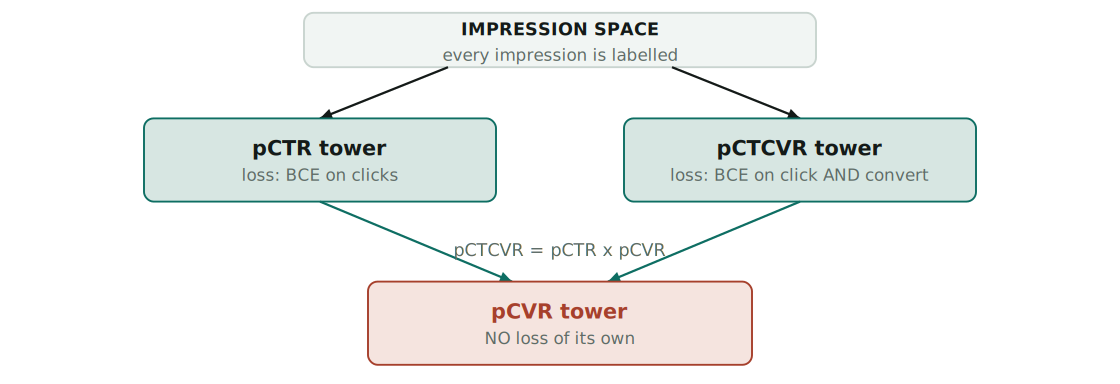
\includegraphics[width=\linewidth]{figures/esmm.pdf}\par\vspace{3pt}
\nopagebreak{\footnotesize\color{muted}Figure 11. ESMM. Both supervised tasks live on the full impression space, so the selection bias is gone and CVR is learned as the ratio. The cost: the product is numerically touchy when pCTR is small, and a miscalibrated CTR tower propagates straight through.\par}\medskip
Both supervised tasks are defined over all impressions, so the bias is gone, and the CVR tower inherits representations from the CTR task which has vastly more data. The caveat to volunteer: the product is numerically touchy when pCTR is small, and a miscalibrated CTR tower propagates straight into CVR.\par
\csubsection{Delayed feedback}
A conversion can land hours or days after the click. So at training time a ``negative'' might just be a conversion that has not happened yet, and your label is a function of how long you waited.\par
Three things I would do. Pick an attribution window from the actual conversion delay distribution --- measure it, do not guess; in most commerce categories the bulk lands within 24 hours but considered purchases have a long tail. Treat recent unconverted clicks as censored rather than negative, and either exclude the most recent window from training or use a delayed-feedback model that jointly models conversion and delay. And retrain often enough that the censoring window is a small fraction of your training period.\par
The failure if you ignore it: your model systematically under-predicts CVR on exactly the most recent data, which is the data most representative of now.\par
\csubsection{Position bias, and how you actually estimate the propensities}
Your labels came out of a ranked list, so a click at rank 1 and a click at rank 20 are not equivalent evidence. Rank 1 gets examined regardless. Train on raw clicks and you learn the ranking you already had --- the model's strongest discovered feature becomes ``where did the old ranker put this,'' and good new items can never rise. It is a self-fulfilling loop and it is the reason a ranker can look excellent offline and never improve anything.\par
The standard correction is inverse propensity scoring: weight each example by one over the probability that the user examined that position. The interesting part is where the propensities come from, and there are three answers with very different costs.\par
\textbf{RandPair --- swap two positions at random on a slice of traffic.} Unbiased and simple. It is also the one that hurts, because you are deliberately showing worse results. I would run it on a fraction of a percent as a calibration reference, not as the production mechanism.\par
\textbf{Intervention harvesting --- free, and the one I would build.} You are already running A/B tests, and different rankers put the same query-item pair at different positions. That is randomisation you have already paid for. Mine the existing experiment logs for pairs that appeared at multiple positions and take the click-rate ratio across positions. Zero additional user cost, and at 200 QPS over six months there is plenty of it.\par
\textbf{Jointly estimate propensity and relevance from clicks} --- regression-EM, or a dual-tower examination model where one tower sees only position and layout features and the other sees query-item features. No randomisation at all. The catch is identifiability: without genuine position variation in the logs the examination tower simply absorbs relevance and you have learned nothing. Check it, do not assume it.\par
Three refinements worth naming, because they are where the textbook answer stops and production begins.\par
\textbf{Position is not one number on a grid.} A mobile app shows a two-column grid, so examination depends on row, column, device, and whether the item was above the fold on that screen size. Condition the propensity on layout, not on a rank index. Getting this wrong on mobile is worse than not correcting at all, because the correction is confidently wrong.\par
\textbf{Trust bias is separate from examination bias.} Users click top-ranked results partly \textit{because} they are top-ranked --- they trust the ranking --- not only because they looked. IPS on examination alone does not remove that, and the fix is a click model that has a separate trust term per position.\par
\textbf{IPS has a variance problem.} Small propensities produce enormous weights, a handful of examples dominate the gradient, and validation metrics oscillate. Clip the weights, which trades a little bias for a lot of variance; or use self-normalised IPS; or go doubly robust, combining IPS with a learned reward model so you are only exposed to variance where the reward model is wrong. Always report effective sample size alongside anything IPS-weighted.\par
\csubsection{Calibration}
If you multiply pCVR by price, pCVR must be a probability, not a score. A model that ranks perfectly but is systematically 3x over-confident produces a completely wrong expected-value ordering as soon as prices vary.\par
So: reliability diagrams on held-out data, ECE as a tracked metric, and a post-hoc calibration map --- Platt or isotonic on a held-out set --- refit on a schedule. Report calibration per price decile and per category, because aggregate calibration hides the segments where it is broken.\par
\csection{The ranking model}
\par\noindent{\small\setlength{\tabcolsep}{4pt}%
\begin{tabularx}{\linewidth}{YYY}\hline
\textbf{Head} & \textbf{Loss} & \textbf{Feeds} \\ \hline
pCTR & BCE on clicks over all impressions & the EV product \\
pCVR & none directly --- learned through ESMM's product & the EV product \\
pRel & listwise, or distilled from the cross-encoder & the relevance gate \\
pReturn & BCE on returns among purchases & the penalty term \\
\hline\end{tabularx}}\par\medskip
Shared bottom first. Escalate to MMoE and then PLE only when you have \textit{measured} negative transfer --- each head against a single-task model trained alone. Task loss weighting usually dominates the architecture choice anyway.\par
\begin{decide}{GBDT or neural for the L2?}
\drow{CHOSE}{Both -- a neural model produces user-history and query-item embeddings offline, and those enter a LambdaMART/LightGBM ranker as features}
\drow{OVER}{Pure neural, or pure GBDT}
\drow{WHY}{200 heterogeneous engineered features is tree territory -- scale-invariant, minutes to train on CPU, monotonic constraints available, legible importances. Representation learning over raw IDs and history sequences is not, and trees cannot do it.}
\drow{COST}{two training pipelines and an embedding-freshness dependency}
\drow{BUT}{multi-task goes neural first, because a GBDT does not do multi-task cleanly and ESMM needs shared representations}
\end{decide}
\textbf{Which model.} For an L2 with \textasciitilde{}200 engineered tabular features, LambdaMART on LightGBM is the strong default: minutes to train on CPU, scale-invariant, monotonic constraints available when you need to guarantee that a higher-rated product never ranks lower for that reason, and legible feature importance when a PM asks why something ranked where it did. Neural wins when the signal is in raw high-cardinality IDs and user history sequences. The honest production answer is both: a neural model produces user-history and query-item embeddings offline, and those become features in the GBDT.\par
Multi-task is the one place I would go neural first, because a GBDT does not do multi-task cleanly and ESMM needs shared representations.\par
\textbf{Features, in four groups.} Query-item match: BM25 per field, dense cosine, the arm ranks, category agreement, attribute overlap. Item: price percentile within category, rating, review count, seller quality, delivery speed, stock, image count. Query: frequency bucket, predicted category, length, intent. User and context: history embedding, price sensitivity, device, surface, time.\par
\textbf{The freshness trap.} The behavioural features --- historical CTR and CVR for a query-item pair --- will dominate feature importance and are near-empty on tail queries. Train with explicit missingness rather than imputing zero, so the model can learn a distinct regime instead of reading ``no data'' as ``bad.'' Then bucket your eval by query frequency and check the tail decile specifically, because aggregate NDCG will look fine while the tail falls off a cliff.\par
\csection{The L1/L2 split: how you train the cheap model}
Everyone draws the two-stage ranker and almost nobody says how L1 is trained, which is a shame because the answer is interesting and it mirrors retrieval.\par
L1's job is \textbf{not} to rank well. Its job is to not throw away anything L2 would have wanted. So do not train it on clicks --- train it to \textbf{imitate L2}. Score a large sample of candidates with L2 offline, and fit L1 to reproduce L2's ordering, or at minimum L2's top-k membership. That is distillation, and it is the right objective because it is literally the thing L1 is for.\par
Which means the metric for L1 is \textbf{recall of L2's top-k}, not NDCG. If L1 keeps 98\% of what L2 would have put in the top 100, L1 is doing its job regardless of how it orders them. Reporting NDCG for L1 is the same category error as reporting NDCG for retrieval.\par
Keep it genuinely cheap: a small tree ensemble or a linear model over a feature subset that avoids anything requiring a remote fetch. The moment L1 needs the same features as L2, it has stopped being a filter and you have paid for two L2s.\par
\csection{Features, freshness, and the skew that eats rankers}
Four groups, and roughly two hundred of them for a commerce ranker. \textbf{Query-item match}: BM25 per field, dense cosine, each retrieval arm's rank and score, category agreement, attribute overlap. \textbf{Item}: price percentile within category, rating, review count, seller quality, delivery speed, stock, image count, age. \textbf{Query}: frequency bucket, predicted category, length, intent class. \textbf{User and context}: history embedding, price sensitivity, device, surface, hour, session depth.\par
Three failure modes matter more than the feature list.\par
\textbf{Point-in-time correctness.} The single largest source of leakage in ranking is computing a feature using data from after the impression. A ``30-day item CTR'' computed at training time from a table built today includes clicks that happened \textit{after} the impression you are training on --- including the click you are trying to predict. The model learns a feature it cannot have at serving time and offline metrics look wonderful. Your feature store must support as-of joins, and you must test them.\par
\textbf{Log the features, do not recompute them.} The robust fix for training-serving skew is to log the exact feature vector the model scored at request time, and train on those logged values. Then skew is impossible by construction: whatever was wrong at serving is equally wrong at training, so the model learns around it.\par
\par\vspace{6pt}\noindent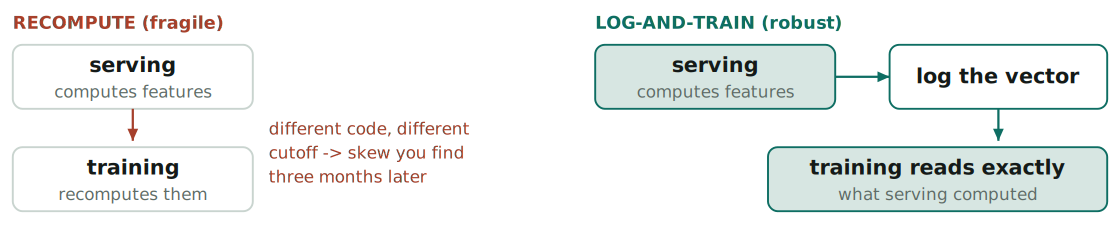
\includegraphics[width=\linewidth]{figures/skew.pdf}\par\vspace{3pt}
\nopagebreak{\footnotesize\color{muted}Figure 13. Logging the served feature vector removes training-serving skew by construction -- whatever was wrong at serving is equally wrong at training, so the model learns around it. The cost is storage: roughly 200 floats per impression, and you can sample.\par}\medskip
The cost is storage --- you are logging a 200-float vector per impression --- and at this volume that is real but affordable, and you can sample it.\par
\textbf{Behavioural features dominate and are empty on the tail.} Historical CTR and CVR for a query-item pair will top your feature importance chart and be missing for exactly the long-tail queries in the prompt. Train with explicit missingness rather than imputing zero, so the model can learn a separate regime instead of reading ``no data'' as ``bad.'' Then report NDCG by query-frequency decile and make the tail deciles a shipping gate, not a diagnostic you run after someone complains.\par
\csection{Exploration: how a new listing ever gets ranked at all}
This is the closed loop from earlier, and it is a real business problem in a marketplace, not an ML nicety. A new product has no behavioural features, so the ranker scores it low, so it gets no impressions, so it never acquires the features that would let it rank. Sellers notice.\par
Three mechanisms, cheapest first.\par
\textbf{Reserve exposure.} Give new or low-impression items a small guaranteed share of slots --- one slot in the first grid, or a fixed fraction of traffic. Blunt, trivially implementable, easy to measure, and it works.\par
\textbf{Score by an optimistic bound rather than the mean.} The model's uncertainty about a cold item is large; UCB-style, add a term proportional to that uncertainty so unexplored items get a chance in proportion to how little you know. Thompson sampling from the posterior is the cleaner version. This is strictly better than a reserved slot because the exploration is targeted, and strictly harder because you need a calibrated uncertainty estimate.\par
\textbf{Lean on content features.} The same argument as cold-start retrieval: a ranker whose features are mostly behavioural cannot score a new item at all, while one with strong content and embedding features can make a reasonable guess on day zero. ID-feature dropout during training applies here exactly as it does in the item tower.\par
The metric to instrument: \textbf{time-to-first-hundred-impressions for a new listing}, and the conversion rate of items in their first week versus steady state. If new items convert \textit{better} than established ones, your ranker is under-exploring and you are leaving money on the table.\par
\cchapter{The metrics, in full}
She asked about CVR; have the whole board ready, and know which one you would actually ship on.\par
\par\noindent{\small\setlength{\tabcolsep}{4pt}%
\begin{tabularx}{\linewidth}{YYY}\hline
\textbf{Group} & \textbf{Metric} & \textbf{What it is for, and what it hides} \\ \hline
\textbf{Engagement} & CTR & Fast, high-volume, the workhorse. Rewards clickbait thumbnails. \\
 & Click position / MRR of first click & Are good results near the top, not just present \\
 & Add-to-cart rate & Much stronger intent than click, still same-session \\
 & Dwell time / long click & Proxy for satisfaction; needs a threshold you must justify \\
\textbf{Conversion} & CVR per click & The stated objective. Denominator is clicks, so it is blind to whether anyone clicked. \\
 & CVR per search session & The one I would actually ship on. Captures retrieval failure, which per-click CVR cannot see. \\
 & CTCVR & Conversion per impression. The ESMM target, and the honest end-to-end rate. \\
\textbf{Money} & GMV per session & The guardrail that catches the cheap-item pathology \\
 & Revenue / margin per search & If they have margin data, the real objective \\
 & Average order value & Moves opposite to CVR under a pure-CVR ranker; that divergence is the tell \\
\textbf{Relevance} & NDCG@k & Graded, position-discounted, the offline standard. Needs judgements. \\
 & Recall@1000 & The retrieval metric. Measure at the ranker's candidate count. \\
 & Precision@k, MAP, MRR & Binary-judgement cousins; MRR when one right answer exists \\
\textbf{Search health} & Zero-result rate & The direct tail metric. For this question, a headline number. \\
 & Reformulation rate & The user telling you the results were wrong \\
 & Query abandonment & Search with no click at all \\
 & Clicks below the fold & Did they have to hunt \\
\textbf{Long-term} & Return / cancellation rate & A CVR win that raises returns is a loss \\
 & Repeat purchase, next-session return & The only real measure of satisfaction \\
 & Catalogue coverage, exposure Gini & Marketplace supply health; a concentrating ranker kills sellers \\
\textbf{System} & p50 / p99 latency & Latency is a quality metric --- measure CVR against it \\
 & ECE, calibration ratio & Required if you multiply probabilities by price \\
\hline\end{tabularx}}\par\medskip
\begin{calloutsay}I would ship on CVR per search session, with GMV per session and return rate as guardrails that cannot regress, and report tail zero-result rate separately because it is the thing this system is being built to fix.\end{calloutsay}
\cchapter{Mobile versus web}
She specified a mobile app search bar. Being able to say precisely how the web version differs is cheap signal that you have built both.\par
\par\vspace{6pt}\noindent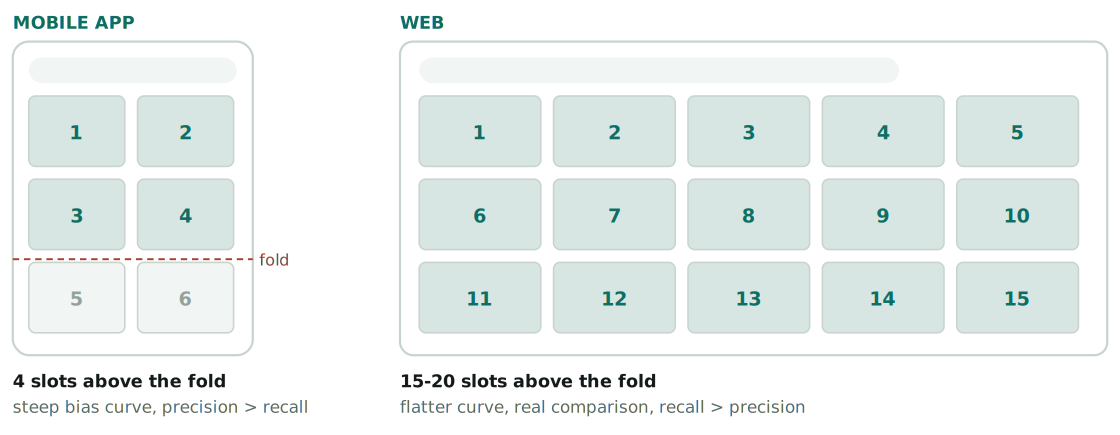
\includegraphics[width=\linewidth]{figures/surfaces.pdf}\par\vspace{3pt}
\nopagebreak{\footnotesize\color{muted}Figure 14. Four slots above the fold against fifteen to twenty. The consequence to state out loud: estimate propensities \textit{per surface}, because one shared curve is confidently wrong on both.\par}\medskip
\textbf{Position bias is far steeper on mobile}, because four items are visible instead of twenty. Practically: you must estimate propensities \textit{per surface} --- one shared propensity curve is simply wrong --- and the value of getting rank 1 right is much higher on mobile. If you only fix one thing about your training labels, fix this.\par
\textbf{Precision beats recall on mobile, and the reverse on web.} With four slots there is no room for a hedge; showing one wrong item costs a quarter of the visible page. On web, a broader candidate set lets the user do the comparison themselves, so slightly lower precision with better coverage is often the better trade. Concretely, I would run a tighter relevance gate and more aggressive deduplication on mobile.\par
\textbf{Queries are shorter and dirtier on mobile.} Thumb typing means more typos, more abbreviations, and heavier reliance on typeahead and voice. So spell correction and query completion carry more weight on mobile --- and the suggestion ranker becomes a first-class model rather than an afterthought, because a good suggestion converts an ambiguous tail query into a head query before retrieval ever runs. That is the cheapest fix for the problem in the prompt and I would say so.\par
\textbf{Diversity matters more on mobile.} Four near-identical listings --- which a marketplace produces constantly --- is the entire visible page. Deduplication by product identity, not just by listing, is a mobile requirement and a web nicety.\par
\textbf{Latency variance is worse on mobile} because of cellular networks, so the client-side budget is tighter than the server-side one suggests. Prefetching the next scroll page and progressive image loading are part of the design.\par
\begin{decide}{One model for mobile and web, or two?}
\drow{CHOSE}{One ranker with surface as a feature; separate propensity curves; separate diversity and dedup policy}
\drow{OVER}{Two complete stacks}
\drow{WHY}{the model can learn the surface interaction from one pipeline, but the position-bias curves are genuinely different objects and a shared curve is confidently wrong on both}
\drow{COST}{you must evaluate per surface always, or a mobile regression hides under a web win}
\end{decide}
\textbf{How I would handle it in the model.} Surface as a feature first, not separate models --- you keep one training pipeline and the model learns the interaction. Separate models only for the things that are genuinely different objects: propensity curves, definitely; the diversity and dedup policy, probably; the ranker itself, only if a surface-interaction analysis says the shared model is leaving real value behind. And evaluate per surface always, because a shared aggregate metric will hide a mobile regression under a web win.\par
\cchapter{The seam: how retrieval and ranking break each other}
\begin{calloutsay}The ranker is trained on whatever candidate distribution the retriever produced. So if I change retrieval, the ranker's training data is stale, and I would not read the experiment until I had retrained it on logs from the new candidates.\end{calloutsay}
Raise this yourself. It is the part of the question that requires having owned both halves, almost nobody brings it up unprompted, and it is the most direct evidence you can give that you have shipped one of these rather than read about it.\par
\par\vspace{6pt}\noindent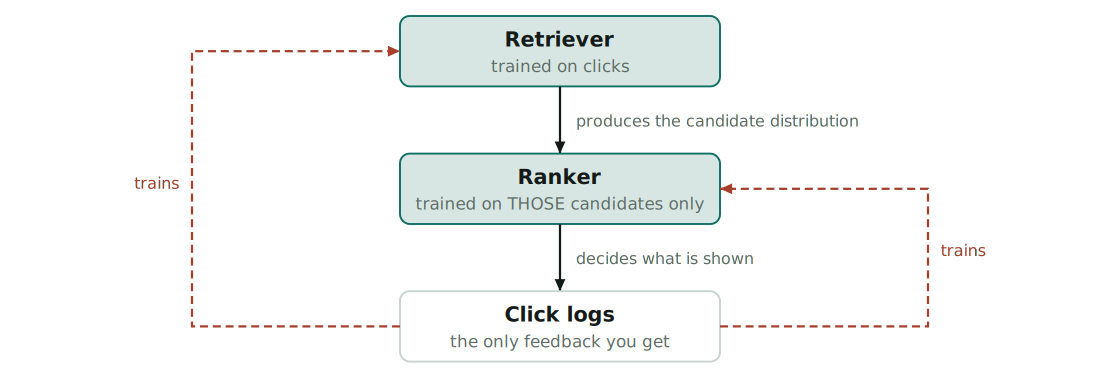
\includegraphics[width=\linewidth]{figures/seam.pdf}\par\vspace{3pt}
\nopagebreak{\footnotesize\color{muted}Figure 15. Change either box and the other one's training data is stale. A 6-point recall win reads as a flat A/B until the ranker has been retrained on the new candidate distribution. Never change both in one experiment.\par}\medskip
\textbf{Ranker trained on retriever v1, served with retriever v2.} The ranker has never seen the newly-surfaced items; they are out of distribution and it scores them conservatively, precisely because they are unfamiliar. So a genuine 6-point recall win shows up as a flat A/B. The fix is sequencing, not modelling: ship the retrieval change to a slice, log the new candidate distribution, retrain the ranker on it, and only then read the experiment. If you tell her this before she constructs the scenario as a gotcha, you have answered the hardest follow-up in the round in advance.\par
\textbf{Retriever trained on positives that the ranker chose to show.} The retriever's positives are clicks, and clicks only happen on items the ranker put on screen. So the retriever is being taught to find what the current ranker likes. Two tightly coupled models, each learning the other's bias. Mitigations: mine positives from deeper ranks and from reformulated sessions, keep an exploration slice whose logs are used preferentially for training, and use propensity weighting on both sides rather than only the ranker.\par
\textbf{Each stage's metric is blind to the other's failure.} Retrieval recall improves while ranking gets worse, aggregate CTR is flat, and each team reports a win. The only honest end-to-end offline measure is NDCG computed over the full pipeline against a judgement set that was \textit{not} pooled from the current system. Measure stage metrics for diagnosis and pipeline metrics for decisions.\par
\textbf{The practical policy I would state.} Never change retrieval and ranking in the same experiment --- you cannot attribute the result. Retrain the ranker on a cadence that is a multiple of the retriever's, always downstream of it. And keep a small always-on randomised slice whose logs are the unbiased sample everything else gets calibrated against; it costs a fraction of a percent of traffic and it is the only thing that stops the whole loop drifting somewhere nobody chose.\par
\cchapter{The follow-up tree}
Everything below is a push she can make. Rehearse the answers out loud; the failure mode in this round is hesitation, not being wrong.\par
\csection{On retrieval training}
\textbf{''How do you set the weight on a purchase versus a click?''} I measure it rather than pick it. Judge a few thousand query-item pairs stratified by action, compute the probability the pair is relevant given each action, and take the log-odds difference against impressions. It comes out far flatter than intuition --- about 2.6 to 1, not 10 to 1 --- because the click already carries most of the relevance evidence and the purchase mostly adds price and availability, which are ranking concerns.\par
\textbf{''Do you treat a returned purchase as a negative?''} For the retriever, barely --- the customer searched, found it and bought it, so it was relevant; the return is usually fit or quality. For the ranker it matters enormously, because a return is negative revenue and negative trust. Returns are a ranking signal, not a retrieval signal.\par
\textbf{''Why aggregate to (query, item) instead of training per event?''} Because the retriever has no user features --- the query tower sees a string. Per-event rows therefore add no information and add popularity skew, since a pair shown a million times would contribute a million gradient steps for a signal its counts already capture. The ranker is the opposite: it has user and context features, so it needs per-impression rows and the unclicked negatives the retriever's table discards.\par
\textbf{''What does your negative strategy cost?''} In-batch negatives are free --- already encoded. Every mined or uniform negative is a full item-tower forward pass, so six explicit negatives per positive turns 4,096 encoder passes per step into about 28,000. The mitigation is caching item embeddings from the last index refresh and recomputing only on the refresh cadence, which is what ANCE does.\par
\textbf{''How do you split?''} By time, never randomly --- the last two weeks are test, because you serve forward in time and a random split leaks the same pair to both sides. And a second, query-disjoint split of whole tail queries, because a time-based split still lets a head query's embedding be learned in the training period and evaluated in the test period.\par
\textbf{''Why a softmax and not MSE?''} Because there is no target. A click is not a similarity of 1.0, so you would have to invent the label, and the model would learn whatever you invented. Beyond that, MSE optimises magnitudes nothing ever reads, and it has no normalisation --- a model that outputs 0.3 for everything has a fine MSE and zero retrieval utility.\par
\textbf{''Why not triplet loss?''} Four things. It sees one negative per step, so the gradient is a noisy estimate of ``beat everything.'' Its margin is an absolute quantity in a space whose scale the model controls, so unnormalised it can be satisfied by inflating norms. The hinge switches off once satisfied, so late in training most of the batch contributes no gradient --- hence semi-hard mining. And it collapses more readily. The softmax's temperature does the margin's job relatively rather than absolutely, and it is smooth.\par
\textbf{''Is triplet ever right?''} Yes, for verification rather than retrieval. Contrastive and triplet losses give you a calibrated distance with a usable threshold; a softmax gives you an ordering with no absolute meaning. Catalogue deduplication --- is this seller's listing the same physical product as that one --- is exactly that, and it sits inside this system feeding the slate policy's dedup step. I would train it with a margin loss.\par
\textbf{''Where would you use MSE in this design, then?''} Two places. Distilling the cross-encoder into the bi-encoder, but on the \textit{margin} rather than the raw score, because the teacher's absolute scale is arbitrary and only the ordering transfers. And training L1 to imitate L2, which is the same argument.\par
\textbf{''BPR or RankNet instead?''} They are the pairwise cousins and share triplet's core limitation: one comparison at a time, and no notion that position 1 matters more than position 50. BPR is the right tool for implicit-feedback recsys with small candidate sets; for retrieval over 10M it is strictly dominated.\par
\textbf{''When would you use a listwise loss on the retriever?''} I would not. Listwise losses need the whole list, and the retriever's ``list'' is the corpus. Listwise belongs where the candidate set is small enough to hold --- the reranker, and the slate layer.\par
\textbf{''Why not just use a cross-encoder for retrieval?''} Cost. A cross-encoder is about a millisecond per pair, and 10M pairs per query is three hours. The two-tower exists so the item side can be precomputed and the query side reduced to one dot product against an index. You pay for it in expressiveness --- the towers never interact --- which is why the cross-encoder comes back as a reranker over 50 candidates.\par
\textbf{''Should the two towers share weights?''} No, for two reasons. Query text and product text are different distributions --- three words of intent versus a hundred words of catalogue copy --- and a shared encoder has to compromise. And sharing throws away the asymmetry: the item tower can be large because it is offline, the query tower must be small because it is online. Sharing forces both to the smaller budget.\par
\textbf{''How do you handle a brand new product with no interaction history?''} This is where the two-tower earns its keep: the item tower is content-based, so a new listing gets a usable embedding from its title and attributes the moment it is indexed. That is a strong argument against pure ID-embedding retrieval in a catalogue with churn.\par
\textbf{''Would you put an item-ID embedding in the item tower?''} Yes, but with ID dropout during training --- randomly mask the ID feature so the model is forced to produce a good embedding from content alone. Then established items get the benefit of their learned ID and cold items degrade gracefully instead of falling off a cliff. Without dropout the model leans entirely on the ID and cold start breaks.\par
\textbf{''What does batch size actually do here?''} It sets the number of in-batch negatives, so it sets the difficulty of the classification task and the quality of the gradient. That is why these models train at thousands and use cross-device negative sharing. Past a point, more random negatives stop helping and mined hard negatives take over.\par
\textbf{''How do you choose the temperature?''} Sweep it, and diagnose on the score distributions rather than the loss --- you want clear separation between positive and negative scores without the positive saturating. Start around 0.05 for normalised embeddings. Too low and the gradient collapses onto the single hardest negative; too high and the softmax is flat and there is no signal. It can be learned with a clamp.\par
\textbf{''What is the ratio of hard to random negatives?''} I would start with a handful of mined hard negatives per positive on top of the full batch as in-batch negatives plus uniform corpus negatives, and tune it. All-hard is a known failure mode --- it over-fits the miner's idea of hard, and it amplifies any false negatives you failed to filter.\par
\textbf{''Your hard negatives are mined from BM25. What happens once the model beats BM25?''} They stop being hard, and you silently stop learning from them. That is why you re-mine from the current model's own index every epoch or two --- the ANCE loop. Static negatives go stale and the training curve looks fine while the model stops improving.\par
\textbf{''How do you know a mined negative is not actually relevant?''} You do not, which is why you filter. Score every mined negative with the cross-encoder teacher and drop anything scoring above the positive. Training on a false negative is worse than training on no negative --- you are explicitly teaching the model that a correct answer is wrong.\par
\textbf{''Why does the logQ correction matter in commerce specifically?''} Because in-batch negatives are sampled from the click stream, so popular items are negatives far more often, and the uncorrected model learns an anti-popularity bias --- it under-retrieves exactly the items that convert. The correction subtracts the log sampling probability from every logit so the penalty is per- occurrence rather than cumulative.\par
\textbf{''What about items that never appear in any batch?''} They are never negatives for anyone, so nothing ever pushes them down, and they can surface spuriously. At 10M products with a long tail this is a large fraction of the catalogue. Fix it with mixed negative sampling --- uniform draws from the full index alongside the in-batch ones.\par
\textbf{''Recall@1000 improved 6 points and online CTR is flat. What happened?''} Most likely the ranker cannot exploit the new candidates. It was trained on the distribution the \textit{old} retriever produced, so the newly-surfaced items are out-of-distribution for it and it scores them conservatively. Retrieval and ranking are coupled: after a retrieval change you must retrain the ranker on logs from the new candidate distribution before you can read the result. The other candidates are that the new recall is on items that were never going to convert, or that your offline positives were biased toward the incumbent.\par
\textbf{''How would you prove the dense arm is earning its latency?''} Ablate it in an interleaving test, and separately measure its unique contribution --- the fraction of clicked or purchased items that only the dense arm retrieved. If that number is small, the arm is paying for overlap with BM25 and should be cut or retrained.\par
\textbf{''What breaks if you retrain the query tower but not the item index?''} Silent garbage. The two towers define a joint space; a query embedded by v2 against items embedded by v1 is meaningless, and nothing errors. Version the model into the index metadata and refuse to serve a mismatch.\par
\csection{On the funnel}
\textbf{''Why three retrieval arms and not two?''} Because they fail on disjoint query populations. If the behavioural arm's unique contribution is small once you have a good dense arm, drop it --- measure, do not assume.\par
\textbf{''What sets the candidate count out of retrieval?''} The ranker's latency budget from one side, and the recall curve from the other. Plot recall against candidate count and find where it flattens; take candidates up to that knee, and then check the knee is in the same place for tail queries, which it usually is not.\par
\textbf{''Where does personalisation enter?''} Ranking first, because it is cheap there and easy to measure. Retrieval only once you have shown that ranking-side personalisation has saturated, because a personalised retrieval arm multiplies your index cost and makes caching much harder.\par
\csection{On ranking}
\textbf{''Pointwise, pairwise or listwise?''} All three, in different places, and the constraint is calibration. The expected-value score multiplies probabilities by price, so pCTR and pCVR must be pointwise and calibrated --- a LambdaMART score cannot be multiplied by a hundred dollars. Listwise belongs in a relevance model feeding the gate, and in a list-context re-ranking layer over the final fifty.\par
\textbf{''Walk me through LambdaRank.''} NDCG is a step function of the ordering so it has no usable gradient. LambdaRank skips defining a loss and writes the gradient directly: the pairwise logistic gradient multiplied by the change in NDCG you would get from swapping that pair. The multiplier is the whole idea --- it makes a swap at ranks 1 and 2 worth far more than one at 50 and 51. Plug those gradients into gradient boosting and you have LambdaMART.\par
\textbf{''You downsampled negatives 100:1. What did that break?''} Calibration. The model now predicts in the downsampled base rate, so every probability is inflated and every multiplication by price is wrong by a constant. Correct it analytically with the keep rate, then verify on a reliability diagram --- do not trust the formula without checking it.\par
\textbf{''How do you train L1?''} By distilling L2, not on clicks. Its job is to not discard anything L2 would have wanted, so the objective is to reproduce L2's ordering and the metric is recall of L2's top-k. Reporting NDCG for L1 is the same mistake as reporting NDCG for retrieval.\par
\textbf{''Your top feature is 30-day item CTR. What could be wrong with it?''} Two things. Point-in-time correctness --- if it is computed from a table built today it contains clicks that happened after the impression, including the one you are predicting, and that is leakage that makes offline metrics look wonderful. And coverage: it is empty on exactly the tail queries this system is being built for, so train with explicit missingness rather than imputing zero.\par
\textbf{''How do you stop the ranker from being a self-fulfilling prophecy?''} Two levers. Propensity-weight the training labels so a click at rank 1 is not treated as the same evidence as a click at rank 20. And explore: reserved exposure for cold items, or an optimism bonus proportional to the model's uncertainty. Without exploration, items the ranker buries generate no data and the error never corrects.\par
\textbf{''A new seller lists a product. When does it first rank?''} Instrument it --- time-to-first-hundred-impressions is a real metric with a real owner. Without exploration the honest answer is ``possibly never,'' which in a marketplace is a supply problem, not an ML problem.\par
\textbf{''Would you use one model for CTR and CVR or two?''} ESMM, which is neither: two supervised heads on the full impression space, CTR and CTCVR, with CVR learned implicitly as the ratio and never given a loss of its own. That removes the sample selection bias and gives the CVR tower a representation trained on far more data.\par
\textbf{''MMoE or shared-bottom?''} Shared-bottom first, and measure each head against a single-task model trained alone. A drop is negative transfer and that is your signal to escalate to MMoE, then PLE. Escalating without the measurement gets you four times the parameters and no gain. And task loss weighting usually dominates the architecture choice anyway.\par
\textbf{''Your pCVR is well-ranked but badly calibrated. Does it matter?''} It does the moment you multiply it by price. A systematic 3x over-confidence produces a completely wrong expected-value ordering while AUC looks fine. Fix with a post-hoc monotone map on held-out data, refit on a schedule, and report calibration per price decile and per category because the aggregate hides the broken segments.\par
\csection{On CVR specifically}
\textbf{''Why not just train on purchases?''} Sixty million purchases across ten million products is far too sparse, especially on the tail, which is what the question is about. Train on clicks for volume, weight by the downstream action.\par
\textbf{''How long is your attribution window?''} Measured from the conversion delay distribution rather than chosen. And whatever it is, recent unconverted clicks are censored, not negative --- either exclude the most recent window or model the delay.\par
\textbf{''Your pCVR is well-ranked but badly calibrated. Does it matter?''} It does the moment you multiply it by price, which the expected-value objective does. Then a systematic 3x over-confidence produces a completely wrong ordering. Fix with a post-hoc monotone map on held-out data; it barely moves AUC by construction.\par
\textbf{''MMoE or shared-bottom?''} Shared-bottom first, and measure each task head against a single-task model trained alone. If a task is worse in the joint model that is negative transfer and you escalate to MMoE, then PLE. Escalating without that measurement gets you four times the parameters and no gain.\par
\csection{On serving}
\textbf{''You are over your latency budget. What do you cut?''} L2 candidate count first --- 1000 to 500 is usually under a point of NDCG for half the ranking cost, the best exchange rate in the system. Then quantise or distil the ranker. Then \texttt{ef\_search}. Retrieval depth last, because that is the only cut that loses recall permanently. And never a silent timeout that drops an arm.\par
\textbf{''Would you cache?''} Yes, for cost and for median latency --- but say clearly that it does not help p99, because p99 is the tail and the tail is what misses the cache. And in commerce the cache has a correctness problem: price and stock change constantly, so cache the ranked ID list and hydrate price and availability at request time rather than caching rendered results.\par
\textbf{''How do you handle filters at 2\% selectivity?''} In-traversal filtering rather than post-filtering, and below a measured selectivity crossover, brute force over the filtered subset. A few hundred thousand exact dot products beat approximate search over ten million.\par
\csection{On evaluation}
\textbf{''How do you build a judgement set for tail queries?''} Sample by query frequency band, not uniformly, or you will get a head-only set. Judge with an LLM calibrated against a human gold set, benchmarked on human-human agreement rather than on perfect agreement, with a weekly human audit to catch drift.\par
\textbf{''Offline NDCG is up and the A/B is flat. What is your first move?''} Check that the judgement set is not stale relative to the catalogue, then check whether the gain is concentrated in a segment that carries little traffic, then check for a presentation-layer difference the offline metric cannot see. And check statistical power before concluding ``flat'' --- most flat results are underpowered.\par
\textbf{''How much traffic do you need to detect a 1\% relative CVR lift?''} Ask for the baseline rate, then size it. At a 2\% baseline CVR, detecting a 1\% relative lift at 80\% power and alpha 0.05 needs on the order of tens of millions of sessions per arm. State that you would compute it rather than guess, and that if the required sample is implausible you switch to interleaving for the ranking comparison.\par
\cchapter{What I would build first}
The sequencing question is where Staff shows. Four quarters, and each one ends with something measurable.\par
\textbf{Q1 --- instrumentation and the cheap wins.} You cannot improve what you cannot measure, and this system has been running for six months with no tail segmentation. Build the judgement set stratified by query frequency, start reporting zero-result rate and recall by frequency decile, and stand up interleaving. In parallel ship the two cheapest quality wins: the category gate with confidence thresholding and a behavioural synonym layer mined from the logs. Both are days of work and both move tail queries.\par
\textbf{Q2 --- the dense arm, v1.} Two-tower trained with in-batch negatives, the logQ correction, and mixed negative sampling. RRF fusion with BM25. HNSW over 10M int8 vectors. Ship behind interleaving and measure unique contribution on tail queries. This is the single biggest expected move on the stated problem.\par
\textbf{Q3 --- make it good.} Train the cross-encoder. Use it three ways: false-negative filtering, distillation into the bi-encoder, and adaptive-depth reranking for positions 7+ off the blocking path, per Option C. Add ANCE hard-negative refresh. Replace RRF with a learned L1 fusion.\par
\textbf{Q4 --- the objective.} Multi-task ranker with ESMM, delayed-feedback handling, calibration, and the expected-value objective with a relevance gate. This is last not because it is unimportant but because until retrieval is fixed, the ranker is reordering a bad candidate set.\par
If she asks what you would do with one engineer for one month instead: the category gate and the synonym layer, and the tail measurement that proves the rest is worth funding.\par
\cchapter{The whiteboard, in order}
What to draw, when, and the numbers to have on the board. Practise the first three until they come out without thinking.\par
\par\noindent{\small\setlength{\tabcolsep}{4pt}%
\begin{tabularx}{\linewidth}{YYY}\hline
\textbf{Minute} & \textbf{Draw} & \textbf{Say while drawing} \\ \hline
5 & \textbf{The funnel} (Fig 1) & Label each box with its millisecond budget \\
10 & \textbf{Query decomposition} (Fig 3) & Why BM25 fails on the prompt's own example \\
15 & \textbf{The two towers} (Fig 4) & Draw them \textit{different sizes}, and say why \\
18 & \textbf{The weight pipeline} (Fig 4b) & If she asks how positives are chosen --- counts, calibrated values, propensity \\
20 & \textbf{The loss} (Fig 5) & Write it out; this is the retrieval assessment \\
22 & \textbf{What each loss sees} (Fig 5b) & Only if she asks why not triplet or MSE --- four sketches, thirty seconds \\
24 & \textbf{logQ correction} (Fig 6) & One line under the loss \\
32 & \textbf{The EV objective} (Fig 8) & The pivot from retrieval to ranking \\
38 & \textbf{LambdaRank's lambda} (Fig 10) & And why you still need calibrated pointwise heads \\
44 & \textbf{ESMM} (Fig 11) & Only if she pushes on CVR data \\
50 & \textbf{The seam} (Fig 15) & Raise it yourself; it is the highest-signal moment \\
\hline\end{tabularx}}\par\medskip
Figures 7, 9, 12, 13 and 14 are worth knowing but not worth board time unless she asks --- the training pipeline, the downsampling correction, log-and-train, the multi-task head, and the mobile/web comparison.\par
Numbers to have in your head, not on a slide:\par
\begin{calloutnum}10M x 256-d int8 = 2.6 GB of vectors plus \textasciitilde{}2.6 GB of HNSW graph. 20 requests in flight at 200 QPS and 100 ms. Six months = \textasciitilde{}3B searches, \textasciitilde{}1.2B clicks, \textasciitilde{}60M purchases. Cross-encoder over 50 candidates = 10-15 ms on a T4. Clicked impressions are 1-5\% of all impressions. \textasciitilde{}100 impressions per click. Temperature \textasciitilde{}0.05, batch size in the thousands, embedding dim 256.\end{calloutnum}
\begin{itemize}
\item 10M x 256-d int8 = \textbf{2.6 GB} of vectors, plus \textasciitilde{}2.6 GB of HNSW graph at M=32
\item \textbf{20 requests in flight} at 200 QPS and 100 ms
\item 6 months at 200 QPS = \textbf{\textasciitilde{}3B searches, \textasciitilde{}1.2B clicks, \textasciitilde{}60M purchases}
\item Cross-encoder over 50 candidates = \textbf{\textasciitilde{}10--15 ms} on a T4-class GPU
\item Clicked impressions are \textbf{1--5\%} of all impressions --- the CVR data problem
\item \textasciitilde{}\textbf{100 impressions per click}, which is why you downsample negatives
\item Temperature \textbf{\textasciitilde{}0.05}; batch size \textbf{thousands}; embedding dim \textbf{256}
\end{itemize}
\cchapter{Ten things that would lose this round}
\textbf{On retrieval}\par
\begin{itemize}
\item Drawing two identically-sized towers, and not knowing why they differ.
\item Saying ``in-batch negatives'' and stopping, without the sampling bias.
\item Quoting Recall@10 as the retrieval metric.
\item Claiming offline recall against logged clicks is an unbiased evaluation.
\end{itemize}
\textbf{On ranking}\par
\begin{itemize}
\item Accepting ``optimise CVR'' without naming the cheap-item pathology.
\item Answering ``listwise, obviously'' without noticing that the expected-value objective needs calibrated probabilities a LambdaMART score cannot give you.
\item Training on raw clicks with no propensity correction, then wondering why the model's best feature is the old ranker's output.
\item Having no answer for how a brand-new listing ever gets its first impression.
\end{itemize}
\textbf{On both}\par
\begin{itemize}
\item Spending fifteen minutes on sharding a 10M-item index that fits in RAM.
\item Treating retrieval and ranking as two independent problems, and having nothing to say when a recall win produces a flat A/B.
\end{itemize}
\cchapter{The AI-powered search question}
This is the sibling of the set-piece. Nobody has reported Siwen asking it, so treat the wording below as constructed rather than verbatim --- but it is the question her round turns into the moment you say the word ``LLM'' out loud, and every org running a 10M-product search stack in 2026 is being asked some version of it internally.\par
\begin{callout}\textbf{Take the same search stack and make it AI-powered.} Same catalogue and traffic as before --- 10M products, 200 QPS, 100 ms end-to-end p99, six months of logs --- but now you have an LLM budget. Where does the LLM go: query understanding, retrieval, ranking, relevance judgement, or the answer surface? What do you refuse to let it touch, and how do you prove any of it worked?\end{callout}
\csection{What is actually being tested}
Not whether you can name a model. Four things:\par
\textbf{Can you place an LLM by latency tier rather than by enthusiasm.} The single discriminating question in this round is \textit{where the call happens}. Offline, near-line, online-from-cache, and online-blocking are four different systems with four different cost models, and most candidates collapse them into one.\par
\textbf{Do you know that the highest-leverage LLM use in search is not in the serving path at all.} It is the catalogue and the judgement set. Both are offline, both are unbounded in latency, and both move tail recall more than any reranker will.\par
\textbf{Do you know what not to do.} Generative retrieval over a 10M-item catalogue that changes daily, a listwise LLM reranker inside a 100 ms budget, an answer surface on a transactional query --- each of these is a plausible-sounding answer that a senior person rules out in one sentence with a number attached.\par
\textbf{Can you prove it worked.} ``The LLM judge says relevance is up 8\%'' is not a result, and knowing why is most of the difference between an L5 and an L6 answer here.\par
\begin{callouttrap}The phrase ``AI-powered search'' tempts you into putting the model in the serving path, because that is where it is visible. The best answers spend the first twenty minutes offline -- on the catalogue and on labels -- and only then ask what is left that has to happen at query time.\end{callouttrap}
\csection{The first five minutes: what to ask}
\begin{enumerate}
\item \textbf{''Is the 100 ms budget unchanged?''} If yes, then no LLM call happens in the blocking path except as a cache lookup, and I will design around that. \textit{Assume unchanged unless told otherwise, and say you are assuming it.}
\item \textbf{''What is the cost envelope --- per query, or per month?''} At 200 QPS a per-query call is \textasciitilde{}520M calls a year. A per-item offline pass is 10M calls, once. Those are different businesses and the answer changes with it.
\item \textbf{''Is the deliverable better products, or an answer?''} A ranked grid and a generated answer are different surfaces with different metrics, and in commerce the answer surface can cannibalise the grid.
\item \textbf{''Do we own the catalogue text, and can we write back to it?''} This decides whether the biggest lever is available at all.
\end{enumerate}
If you get a fifth: ask what languages. Multilingual query understanding is where LLMs are most clearly better than the pipeline they replace, and it is the easiest win to under-claim.\par
\csection{Numbers you derive from the prompt, out loud}
Say the token math before anyone asks for it. Rates vary by model and vendor and change often, so carry the \textit{formula} and one worked example at a stated assumption rather than a memorised price.\par
\par\noindent{\small\setlength{\tabcolsep}{4pt}%
\begin{tabularx}{\linewidth}{YYY}\hline
\textbf{Workload} & \textbf{Derivation} & \textbf{Volume} \\ \hline
Catalogue enrichment, one pass & 10M items, \textasciitilde{}600 in + 150 out & 6B in, 1.5B out \\
Re-enrichment, steady state & \textasciitilde{}1\% of catalogue changes daily & 60M in, 15M out per day \\
Judgement set, 50k pairs & 50k, \textasciitilde{}400 in + 80 out & 20M in, 4M out \\
Distillation labels, 5M pairs & 5M, \textasciitilde{}400 in + 20 out & 2B in, 100M out \\
Query rewrite, every query & 200 QPS, \textasciitilde{}150 in + 60 out & 2.6B in per 6 months \\
Query rewrite, cached head+torso & Precompute top 200k queries once & 30M in, 12M out \\
\hline\end{tabularx}}\par\medskip
The last two rows are the whole argument. Rewriting every query costs roughly a thousand times what precomputing the queries that matter costs, for a gain that lands almost entirely on the tail --- which is exactly the part a cache misses. The resolution is not ``cache or not'', it is a tiered policy, below.\par
\begin{calloutnum}A per-query LLM call at 200 QPS is \textasciitilde{}17M calls a day. A one-time catalogue pass is 10M calls, ever. If the per-query call is not measurably better than a distilled student model, it does not ship.\end{calloutnum}
\csection{The sixty minutes}
\par\noindent{\small\setlength{\tabcolsep}{4pt}%
\begin{tabularx}{\linewidth}{YYY}\hline
\textbf{Minutes} & \textbf{What} & \textbf{Why} \\ \hline
0-5 & Clarify, state the latency tier framing & Establishes the organising idea immediately \\
5-12 & The tier table and the system diagram & Everything later is ``which tier is this in'' \\
12-25 & \textbf{Offline: catalogue enrichment and the judgement flywheel} & The two biggest levers, and the ones most candidates skip \\
25-35 & Query understanding, cached, with the fallback & Where the prompt's tail example actually gets fixed \\
35-45 & \textbf{Retrieval and reranking: teacher offline, student online} & The distillation answer is the whole point \\
45-52 & The answer surface, and when not to build it & Product judgement, not modelling \\
52-60 & Evaluation, cost, what you would build first & Staff signal \\
\hline\end{tabularx}}\par\medskip
\cchapter{The system: five tiers, and everything goes in one of them}
Draw this table before you draw any boxes. It is the answer to the question, and every later section is an instance of it.\par
\par\noindent{\small\setlength{\tabcolsep}{4pt}%
\begin{tabularx}{\linewidth}{YYYY}\hline
\textbf{Tier} & \textbf{Budget} & \textbf{What belongs here} & \textbf{What it costs} \\ \hline
Offline batch & Hours to days & Catalogue enrichment, synthetic queries, judgement sets, distillation labels & Pipelines and versioning \\
Near-line & Seconds to minutes & New-item enrichment, warming the rewrite cache for emerging queries & A queue and a staleness budget \\
Online, cached & Under 1 ms & Rewrites and expansions for head and torso queries, looked up & Cache size, and a fallback \\
Online, blocking & 10-30 ms & A distilled cross-encoder. Not an LLM API call & GPU or a quantised CPU model \\
Never & --- & Ungrounded generation about price, stock, safety or sizing & Trust, and in commerce, liability \\
\hline\end{tabularx}}\par\medskip
\par\vspace{6pt}\noindent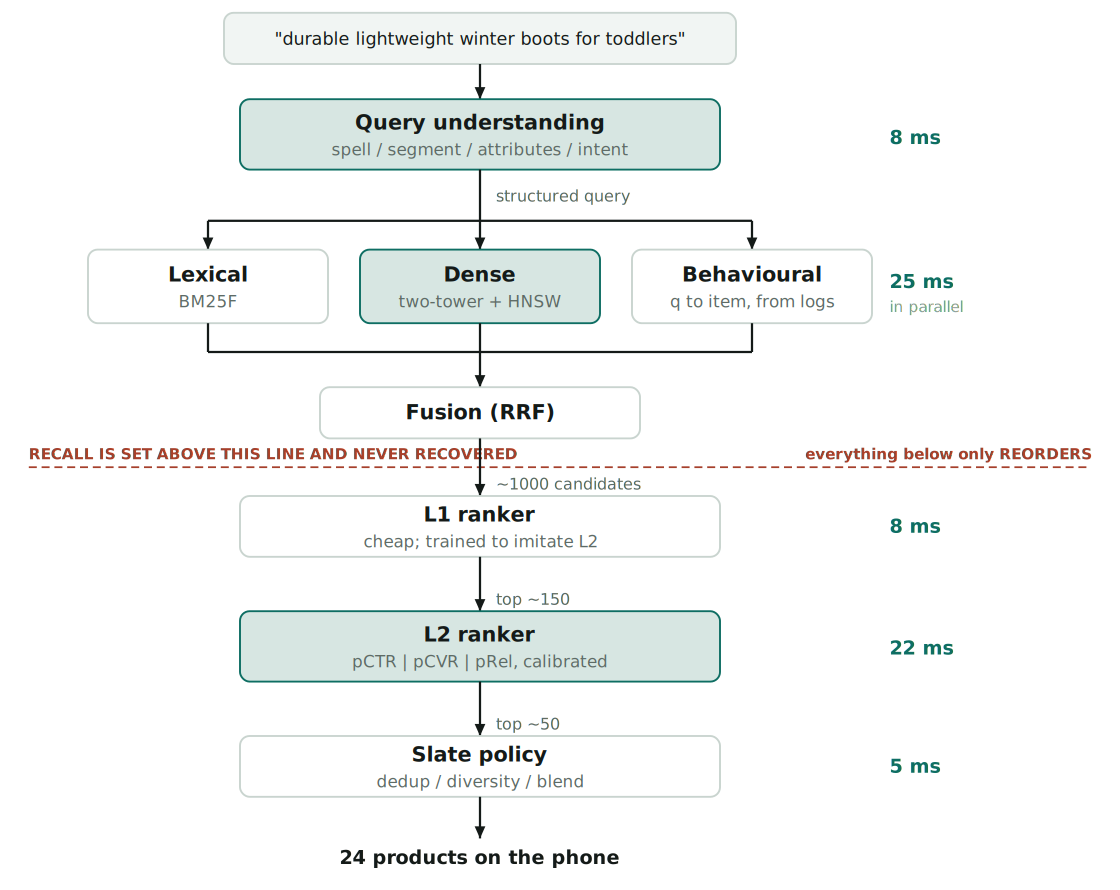
\includegraphics[width=\linewidth]{figures/funnel.pdf}\par\vspace{3pt}
\nopagebreak{\footnotesize\color{muted}Figure 1. The funnel, unchanged. The point of this round is that almost nothing in the serving path becomes an LLM call. What changes is the quality of the inputs each box receives.\par}\medskip
\begin{decide}{Where does the LLM go first?}
\drow{CHOSE}{Offline -- catalogue enrichment and the judgement set}
\drow{OVER}{Online, as a query rewriter or a reranker, which is what the phrase ``AI-powered search'' tempts you into}
\drow{WHY}{both are unbounded in latency, both are paid once per item rather than once per query, and both move tail recall -- which is the stated problem -- while a reranker only reorders a candidate set that was already missing the item}
\drow{COST}{enrichment pipelines, a re-enrichment story every time the prompt or the model version changes, and a human audit sample you have to keep funding}
\drow{DROP IT IF}{the catalogue text is already clean and structured, in which case the labels are the only offline lever left and you skip straight to the judgement flywheel}
\end{decide}
Three things to say while you draw it.\par
\textbf{The serving path barely changes.} Query understanding, three retrieval arms, fusion, L1, L2, slate policy. What changes is that every box gets better inputs: cleaner item text, better labels, better teachers.\par
\textbf{Recall is still set at the top and never recovered.} An LLM reranker cannot retrieve an item the retriever did not return. If the tail query in the prompt fails because the word ``lightweight'' appears nowhere in the item's text, no amount of reranking fixes it --- writing that attribute into the item does.\par
\textbf{Every online LLM call must beat its own distilled student.} That is the bar, and stating it early is what stops the rest of the answer becoming a wish list.\par
\cchapter{Offline, part one: the catalogue is the biggest lever}
Go back to the prompt's own example: \textit{''durable lightweight winter boots for toddlers.''} Four constraints. Ask why the current system fails on it, and the honest answer is usually not a modelling failure at all. The item that should win is a toddler snow boot whose title is \textit{''Kids Winter Snow Boots Waterproof Non-Slip 2024 New''} --- it is 340 grams, it is durable, and neither fact appears anywhere a retrieval system can see. The seller wrote a title for a keyword search engine in 2016.\par
\textbf{So extract the attributes.} For each item, run one pass over title, description, structured seller fields, images and the review text, and emit a constrained JSON record against a fixed, closed attribute vocabulary: age band, weight class, material, water resistance, sole type, closure, and so on.\par
Three places the output lands, and all three matter:\par
\begin{itemize}
\item \textbf{Fielded lexical index.} New BM25F fields with their own weights. This is what fixes ``toddlers'' as a facet rather than a token.
\item \textbf{Item text for the dense encoder.} The two-tower item tower now reads a normalised, attribute-bearing document instead of seller keyword soup, which is a larger quality change to the embedding than any encoder swap.
\item \textbf{Facets and filters in the product surface.} Free, and often the thing the PM notices first.
\end{itemize}
\textbf{Then generate queries for the items nobody searches for.} Synthetic query generation --- doc2query, in the old naming --- asks the model for the 10 to 20 queries a shopper would plausibly type to find this item, and indexes them as an extra field. This is aimed squarely at the zero-engagement tail: the items that have no clicks, therefore no behavioural signal, therefore no presence in any query-to-item table, and, as the set-piece document notes, are never even sampled as negatives. Synthetic queries give the lexical arm something to match and the dense arm something to train on.\par
\begin{decide}{How far do you trust extracted attributes?}
\drow{CHOSE}{Closed vocabulary, confidence-thresholded, verified against the seller's structured fields where they exist, with a human-audited sample every batch}
\drow{OVER}{Free-text extraction written straight into the index}
\drow{WHY}{in commerce a hallucinated attribute is not a relevance bug -- ``waterproof'', ``flame retardant'', ``BPA free'' and a size chart are claims, and a wrong one is a return, a complaint, and sometimes a regulator}
\drow{COST}{coverage is lower than free extraction, and the vocabulary needs maintenance}
\drow{FALLBACK}{when confidence is below threshold, emit nothing rather than a guess, and let the item keep its old behaviour}
\end{decide}
\begin{calloutsay}The cheapest way to improve tail retrieval on a marketplace is usually not a better retriever. It is writing the attributes the shopper searched for into the item, because on a third-party catalogue they are genuinely absent, not merely hard to match.\end{calloutsay}
\textbf{How you measure it, so it is not vibes:} attribute coverage (share of items with a non-null value per attribute), precision on a human-audited sample per attribute, and then the only one that counts --- recall on tail queries, measured by frequency decile, before and after. If coverage goes up and tail recall does not move, the attributes you extracted are not the ones shoppers search with, and the fix is to mine the vocabulary from the query logs rather than from the taxonomy.\par
\cchapter{Offline, part two: the judgement flywheel}
The bottleneck in search quality is almost never model capacity. It is labels. Human relevance judgement costs dollars per pair and takes days; a search team with 5,000 judged pairs makes decisions with error bars wider than every change it ships. This is the part of ``AI-powered search'' that actually compounds.\par
\textbf{The mechanism.} Graded relevance rubric, three or four points, written down and versioned. The model sees the query, the item's enriched text, and the rubric, and returns a grade with a one-line justification. You now have 500,000 judged pairs for what 5,000 used to cost.\par
\textbf{Calibrate it before you believe it.} Keep a human gold set --- a few thousand pairs, stratified by query frequency decile and by grade --- that the judge never sees during prompt development. Report the judge's agreement with human on that set against the right ceiling, which is \textit{human-human agreement}, not perfect. On graded commerce relevance, human-human Cohen's kappa in the 0.6 to 0.7 range is normal, and a judge at 0.6 is therefore at the ceiling, not failing.\par
\textbf{What the judgements buy you, in order of value:}\par
\begin{itemize}
\item \textbf{Training data for the cross-encoder}, which is the model that actually serves. This is the distillation path, below.
\item \textbf{False-negative filtering for the retriever.} The set-piece answer calls this out: a mined hard negative that is actually relevant teaches the model the opposite of what you want. A judge over mined negatives removes them at a scale a human panel never could.
\item \textbf{A regression set you can run on every change}, segmented by query frequency, which is what lets you see that a launch won the tail and lost the head.
\end{itemize}
\textbf{Where the judge is not allowed.} Two places, and naming them unprompted is worth a lot:\par
\begin{itemize}
\item \textbf{Shipping decisions.} Offline judged relevance is a leading indicator, not the outcome. Interleaving and A/B decide, because the judge cannot see whether the customer bought anything.
\item \textbf{Any comparison where the judge shares a failure mode with the thing judged.} If an LLM rewrote the query and an LLM judges whether the results match the rewritten intent, the loop is closed and the number means nothing. Judge against the \textit{original} user query, always.
\end{itemize}
\begin{callouttrap}``Our LLM judge says relevance improved 8\%'' is not a result. The questions are: which prompt and model version, what was its agreement with the human gold set, was the gold set refreshed after the change, and what did interleaving say. A metric whose definition includes a model version is a metric that silently drifts when someone upgrades the model.\end{callouttrap}
\textbf{Version the judge as part of the metric.} Pin model and prompt; a judge upgrade is a metric redefinition and needs a re-baseline of every historical number, exactly like changing the NDCG cutoff. Teams that skip this discover six months of trend line that reflects model releases.\par
\cchapter{Online: query understanding, cached, with an honest fallback}
Now the serving path. The query in the prompt is ambiguous and long-tail, which is precisely the population a cache cannot help and precisely where an LLM helps most. That tension is the content of this section.\par
\textbf{The tiered policy.}\par
\par\noindent{\small\setlength{\tabcolsep}{4pt}%
\begin{tabularx}{\linewidth}{YYYY}\hline
\textbf{Segment} & \textbf{Share of traffic} & \textbf{Policy} & \textbf{Latency} \\ \hline
Head, top \textasciitilde{}10k queries & Roughly half & Precomputed rewrite, reviewed, served from cache & Lookup \\
Torso, next \textasciitilde{}200k & A further quarter or so & Precomputed offline, refreshed weekly & Lookup \\
Tail, everything else & The remainder, and where the money is & Deterministic pipeline now; LLM enrichment queued near-line & No LLM in path \\
Emerging, rising fast & Small but urgent & Near-line: detected by frequency delta, enriched within minutes & No LLM in path \\
\hline\end{tabularx}}\par\medskip
The tail row is the one to defend. You do \textit{not} make a blocking LLM call for a tail query. You serve it with the existing pipeline --- spell correction, segmentation, the attribute gazetteer that the catalogue enrichment just made much better --- and you enqueue the query. The second person to type it, minutes later, gets the enriched version. Tail queries are unique per session but not unique per week, and the repeat rate is high enough that near-line enrichment captures most of the value at none of the latency cost.\par
\textbf{What the model actually emits.} Constrained JSON against a schema, not prose: normalised tokens, extracted attributes mapped to the closed vocabulary, an intent label, a category distribution with confidence. A validator parses it; if it does not parse, you fall back, and the fallback is the current pipeline, not an error.\par
\begin{decide}{Does the rewrite replace the query or join it?}
\drow{CHOSE}{The rewrite becomes an additional retrieval arm, fused}
\drow{OVER}{Replacing the user's query with the rewrite}
\drow{WHY}{a rewrite that drops a constraint is invisible and catastrophic -- ``boots for toddlers'' retrieved for ``winter boots for toddlers size 8'' looks fine in a demo and is a wrong answer. Fusing keeps the original arm's recall as a floor}
\drow{COST}{an extra arm to serve and a fusion layer that has to be learned, not constant}
\drow{DROP IT IF}{measurement shows the rewrite arm's unique contribution is negligible, which does happen on head queries where the original is already precise}
\end{decide}
\textbf{Guard the head.} Almost every LLM query-understanding launch wins the tail and loses the head, because head queries are short, precise, and already handled, so any rewrite is at best neutral and at worst adds a constraint the shopper did not ask for. Make ``no regression on the top 10k queries'' a launch gate, and note that an aggregate metric can sit flat while both segments moved a lot in opposite directions.\par
\cchapter{Retrieval: what ``AI-powered'' does and does not change}
\textbf{Hybrid stays.} Three arms --- lexical, dense, behavioural --- is still the answer, and an LLM does not retire BM25. What changes is that the lexical arm now indexes extracted attributes and synthetic queries, and the dense arm now trains on enriched item text and judge-filtered negatives. Both arms got better without either becoming an LLM.\par
\textbf{Learned sparse is the most underrated option in this round.} SPLADE-style models expand a query and a document into weighted term distributions over the vocabulary and serve out of an ordinary inverted index. You get semantic matching with lexical infrastructure, exact-match behaviour preserved, and --- the part that matters in an interview --- full interpretability, because you can read which expanded terms fired. The cost is real and you should name it: posting lists get much denser, so index size and query latency both rise, which is why the models carry a FLOPS regulariser to keep expansion sparse. On a catalogue with heavy identifier traffic (part numbers, model codes, sizes), this is often the highest ratio of quality gained to infrastructure changed.\par
\textbf{Generative retrieval and semantic IDs: know it, and decline it here.} The framing is seductive --- quantise each item into a short code, then have a sequence model emit the code directly, so retrieval becomes decoding and the ANN index disappears. Three reasons it is not the first thing to ship on this system:\par
\begin{itemize}
\item \textbf{New items.} 10M products on a marketplace with continuous listings. A new item's identifier has no presence in the decoder until you retrain or graft it in; the cold-start story is exactly the population you most need to serve.
\item \textbf{Cost of decoding.} Beam search per query against a 100 ms budget is a much harder sell than one HNSW traversal.
\item \textbf{Evaluation.} Recall at a fixed latency against a strong hybrid baseline, at this corpus size, is not a comparison the published results have settled.
\end{itemize}
Say where it \textit{does} earn its place --- recommendation over a stable corpus, and as a complementary head-query arm --- and move on. Knowing the boundary is the signal.\par
\textbf{Multimodal is a real fourth arm, and it is optional.} Product images carry attributes the text never will, and commerce tail queries are full of visual language. Add a vision-embedding arm only after you have measured the dense arm's unique contribution, and hold it to the same bar: clicked items that only this arm retrieved.\par
\cchapter{Reranking: the teacher is offline, the student serves}
This is where the round is won, and the answer is one sentence: \textbf{an LLM makes the labels, a cross-encoder makes the latency.}\par
The three forms of LLM reranking, and what each costs:\par
\par\noindent{\small\setlength{\tabcolsep}{4pt}%
\begin{tabularx}{\linewidth}{YYYY}\hline
\textbf{Form} & \textbf{What it does} & \textbf{Quality} & \textbf{Cost per query} \\ \hline
Pointwise & Score each item for relevance independently & Good, calibratable & 50 calls, parallelisable \\
Pairwise & Compare two at a time & Better, quadratic & Impractical online \\
Listwise permutation & Emit a reordering of a window, sliding over the list & Best & Hundreds of ms to seconds \\
\hline\end{tabularx}}\par\medskip
Listwise is the strongest and it has two properties people forget. It is \textbf{position-biased inside its own prompt} --- the model over-favours items placed early in the list it is shown --- which is mitigated by permuting and aggregating, and that multiplies an already large cost. And it is \textbf{non-deterministic}, which makes an A/B harder to reason about and makes caching partial.\par
Against a 100 ms end-to-end budget where the cross-encoder gets roughly 10 to 15 ms for 50 candidates, a listwise LLM pass is one to two orders of magnitude out. It does not go in the blocking path. It goes in the teacher seat:\par
\begin{enumerate}
\item Teacher scores a large sample of (query, candidate) pairs offline, drawn from real logged candidate sets so the distribution matches serving.
\item Distil into the \textbf{cross-encoder} --- train on the teacher's scores or its pairwise preferences rather than on clicks, which removes position bias from the label at the source.
\item Distil again into the \textbf{bi-encoder}, which is how teacher quality reaches recall rather than only order.
\item Serve the students. Refresh the teacher's labels quarterly, or whenever the candidate distribution shifts --- which, per the seam section, is every time retrieval changes.
\end{enumerate}
\begin{decide}{Any LLM call at all in the blocking path?}
\drow{CHOSE}{No. Students only, with an asynchronous refresh for a narrow slice}
\drow{OVER}{A listwise LLM reranker on the top 20}
\drow{WHY}{100 ms p99 end to end, and the distilled cross-encoder recovers most of the teacher's ordering at a fiftieth of the latency}
\drow{COST}{a distillation pipeline, and a ceiling set by the teacher rather than by the student}
\drow{FALLBACK}{for low-confidence tail queries, serve the student immediately and stream a re-ordered grid a second later if the async teacher disagrees -- but only if the surface can tolerate re-ordering, which on mobile it usually cannot}
\end{decide}
\begin{calloutpush}``What if I give you 500 ms?'' Then the listwise reranker becomes arguable for the tail only -- route by L1 confidence, cap the window at 20, cache the result keyed on the normalised query so the second occurrence is free, and keep the student as the fallback on timeout. I would still spend the first 500 ms of budget on retrieval breadth rather than reordering, because reordering cannot recover recall.\end{calloutpush}
\cchapter{The answer surface: RAG over your own catalogue}
Product judgement, not modelling, and a senior answer starts by refusing most of the surface area.\par
\textbf{When it helps.} Informational and comparison intent --- \textit{''which toddler winter boots are warmest?''}, \textit{''is this jacket machine washable?''} --- where the shopper is doing research the product grid answers badly. Grounded in the retrieved items and their reviews, it is genuinely better than ten blue products.\par
\textbf{When it hurts.} Navigational and transactional intent, which on a commerce search bar is most of the traffic. Someone typing a brand and a model number wants the item, and putting a paragraph above it costs them a scroll.\par
\textbf{How it plugs in.} It consumes the funnel's output; it is a \textit{rendering} of the retrieved set, not a second retrieval stack. Every claim cites the item or the review it came from. When the retrieved set does not support an answer, the surface says so and shows products instead --- a refusal path that exists and is measured is the difference between a demo and a system.\par
\textbf{The commerce-specific constraints}, which are the part that shows you have shipped one:\par
\begin{itemize}
\item \textbf{Never generate price, stock or delivery claims.} They change between generation and impression, and a cached answer asserting a price that no longer holds is a consumer-protection problem, not a quality problem.
\item \textbf{Never generate safety, medical, or compliance claims} --- flame retardancy, allergen content, age safety ratings. Quote the seller's structured field or say nothing.
\item \textbf{Never block the grid on the answer.} Render products at 100 ms and stream the answer alongside. The answer's latency budget is a rendering concern, not a search concern.
\end{itemize}
\textbf{Measure cannibalisation, not just satisfaction.} The metric set is clicks, add-to-cart, purchase, \textit{and} reformulation rate. An answer that satisfies the shopper without a purchase is a loss for this business unless it demonstrably reduces returns --- which is a real and defensible win, and worth saying, because a well-grounded answer about sizing is one of the few things that does.\par
\cchapter{Evaluation: the part that makes it AI-powered rather than AI-flavoured}
Three layers, each answering a different question, and the failure mode is using one to answer another's question.\par
\par\noindent{\small\setlength{\tabcolsep}{4pt}%
\begin{tabularx}{\linewidth}{YYYY}\hline
\textbf{Layer} & \textbf{Question it answers} & \textbf{Speed} & \textbf{What it cannot tell you} \\ \hline
LLM-judged relevance & Did the results get more relevant & Hours & Whether anyone bought anything \\
Interleaving & Do users prefer B's ordering to A's & Days & Anything about a non-ranking change \\
A/B & Did the business metric move & Weeks & Anything at all on the tail, usually \\
\hline\end{tabularx}}\par\medskip
\textbf{Interleaving is the workhorse for ranking changes} and is dramatically more sensitive than an A/B for the same traffic, because it compares two rankings within a single user's result set rather than across populations. Use it for every reordering change. It does not apply to changes in what is retrieved or in the surface itself, which is the honest caveat.\par
\textbf{Segment everything by query frequency decile.} An aggregate is dominated by the head, where none of this work helps. The entire thesis of an AI-powered search programme is tail quality, and a flat aggregate is the expected result even from a large win.\par
\textbf{The guardrail set that catches the actual failures:} zero-result rate by segment, head-query regression, latency p99 including cache misses, and --- the one people forget --- the share of queries where the rewrite changed the retrieved set at all. If the rewrite fires on 3\% of traffic, then a 20\% improvement on those queries is a 0.6\% improvement, and you should have said so before the readout rather than after.\par
\cchapter{Cost engineering}
The arithmetic that decides the design, stated as a formula so it survives whatever this year's rates are. Let $R_{in}$ and $R_{out}$ be the price per million input and output tokens.\par
\begin{mathbox}\[\text{cost}_{\text{online}} \;=\; \text{QPS}\times 86400 \times p(\text{miss})
\times \left(\frac{t_{in}}{10^6}R_{in} + \frac{t_{out}}{10^6}R_{out}\right)\]\end{mathbox}
At 200 QPS, 150 input and 60 output tokens, a 100\% miss rate is 17.3M calls a day and 2.6B input tokens a day. Push $p(\text{miss})$ to 5\% with the tiered cache and it is 130M input tokens a day --- the same design, a twentieth of the bill. That factor, not the choice of model, is where the cost lives.\par
The levers, in the order they pay:\par
\begin{itemize}
\item \textbf{Cache by normalised query.} The largest single factor, by far.
\item \textbf{Distil.} A student that recovers most of the teacher's quality at a fiftieth of the cost is a cost lever before it is a latency lever.
\item \textbf{Route by segment.} Head queries do not need the big model; they barely need a model.
\item \textbf{Batch the offline work}, and reuse a shared prompt prefix across calls so the rubric and the vocabulary are paid for once rather than per call.
\item \textbf{Small model plus verifier.} Cheap model proposes the extraction, the expensive one adjudicates only the low-confidence tail.
\end{itemize}
\cchapter{The seam, in this version}
The set-piece document's seam is that the ranker is trained on the retriever's output. This system has a second one, and it is worse because it is invisible.\par
\textbf{The judge's blind spots become the system's blind spots.} The LLM judges relevance, which trains the cross-encoder, which filters the retriever's negatives and supplies its distillation targets, which changes what is retrieved, which changes what the judge is asked about next. It is a closed loop with no external signal in it. Two things break the loop: a \textbf{human gold set the judge never trains on and that is refreshed on a schedule}, and \textbf{online metrics as the only shipping authority}. Say this unprompted.\par
\textbf{The rewrite moves the training distribution.} Your retriever was trained on six months of logged raw queries. If the serving path now sends it rewritten, attribute-normalised queries, it is being evaluated off-distribution. Either train on rewritten queries --- which means rewriting the historical log, offline, which you can afford --- or keep the raw query as an arm so the retriever still sees what it knows. This is the same class of bug as the ranker's candidate shift, and almost nobody raises it.\par
\cchapter{The follow-up tree}
\textbf{''Why not just use a big model for everything and cache aggressively?''} Because the cache hit rate on the segment that needs help is low by construction. Head queries cache beautifully and do not need the model; tail queries need the model and do not cache. The tiered policy exists precisely because those two facts point in opposite directions.\par
\textbf{''How do you know the extracted attributes are right?''} Human-audited sample per attribute per batch, with an accuracy bar that is higher for claim-like attributes (waterproof, flame retardant, age rating) than for descriptive ones (colour family, closure type). Below threshold, emit nothing. And cross-check against the seller's structured fields where they exist --- disagreement is a signal about the seller as much as about the model.\par
\textbf{''Your judge agrees with humans only 65\% of the time. Isn't that too low?''} It depends entirely on human-human agreement on the same rubric, which on graded commerce relevance is commonly in that range. If two trained humans agree 68\% of the time, a judge at 65\% is at the ceiling. If they agree 90\%, it is failing. Measuring the ceiling first is the whole answer.\par
\textbf{''Would you fine-tune a model for this?''} For the judge, usually not --- the rubric changes and a prompt is cheaper to iterate. For the cross-encoder and the bi-encoder, absolutely, and that is what distillation is. For query understanding, fine-tune once the schema stabilises, mostly to cut cost rather than to raise quality.\par
\textbf{''What breaks first when you ship all of this?''} The head. Every time. The rewrite fires on a query that was already precise, adds a constraint, and drops the item everyone clicks. Which is why the launch gate is a head-query regression check and why the rewrite is an extra arm rather than a replacement.\par
\textbf{''How would you handle a new attribute the taxonomy doesn't have?''} Mine it from the query logs rather than from the taxonomy: cluster unmatched query tokens by co-occurrence with clicked items, surface the top clusters, and add the vocabulary term. The taxonomy is a lagging indicator of what shoppers search for, and on a marketplace it lags badly.\par
\textbf{''What if latency dropped to 50 ms?''} Nothing in the offline half changes, which is the point. The cross-encoder budget is the first casualty: drop to adaptive-depth reranking on the visible slots only, or quantise the student and cut the candidate set from 50 to 25. The tiered cache and the enrichment are untouched, and that robustness is the argument for the architecture.\par
\textbf{''Is there anything you would not use an LLM for here at all?''} Ranking. The ranking objective is expected value over calibrated probabilities estimated from biased feedback, and that is a job for models trained on your logs with propensity corrections, not for a language model's judgement. An LLM can supply a relevance \textit{feature} and a relevance \textit{gate}. It should not supply the score.\par
\cchapter{What I would build first}
\textbf{Q1 --- the judgement flywheel and the measurement it unlocks.} Rubric, human gold set, calibrated judge, 100k judged pairs stratified by query frequency. Stand up per-decile recall reporting and interleaving. Nothing else on this list is provable without it, and it is weeks of work rather than quarters.\par
\textbf{Q2 --- catalogue enrichment.} Attribute extraction into a closed vocabulary, fielded BM25F weights, enriched item text for the dense tower, synthetic queries for the zero-engagement tail. Measure tail recall by decile. This is the biggest single expected move on the stated problem, and it needs Q1 to be visible.\par
\textbf{Q3 --- the serving path, cheaply.} Precomputed rewrites for head and torso, near-line enrichment for emerging queries, the rewrite as a fused arm with a head-regression gate. In parallel, distil the teacher into the cross-encoder using Q1's labels, and use the judge to strip false negatives from the retriever's hard-negative mining.\par
\textbf{Q4 --- the surface, if the data says so.} Learned sparse as a fourth arm if identifier traffic is hurting, and the answer surface \textit{only} for the informational query segment, gated behind a cannibalisation readout.\par
With one engineer for one month instead: the judge and the human gold set, and the tail-recall-by-decile report. It costs almost nothing and it is what makes every subsequent argument fundable.\par
\cchapter{The whiteboard, in order}
\par\noindent{\small\setlength{\tabcolsep}{4pt}%
\begin{tabularx}{\linewidth}{YYY}\hline
\textbf{Minute} & \textbf{Draw} & \textbf{Say while drawing} \\ \hline
5 & \textbf{The five tiers} & Every later answer is ``which tier is this in'' \\
8 & \textbf{The funnel} (Fig 1) & Note how little of it becomes an LLM call \\
14 & \textbf{The enrichment pipeline} & Item text in, closed-vocabulary JSON out, three destinations \\
20 & \textbf{The judgement flywheel} & Judge, gold set, cross-encoder, negatives -- and where the loop closes \\
30 & \textbf{The tiered query policy} & Head cached, tail deferred to near-line, fallback always the old pipeline \\
38 & \textbf{Teacher and student} & The one sentence that answers the reranking question \\
50 & \textbf{The three evaluation layers} & And which question each one cannot answer \\
\hline\end{tabularx}}\par\medskip
\begin{calloutnum}10M items x \textasciitilde{}750 tokens is one 7.5B-token offline pass, paid once. 200 QPS is 17M calls a day if you do it per query. Head+torso is \textasciitilde{}200k distinct queries covering most traffic. Cross-encoder over 50 candidates is 10-15 ms; a listwise LLM pass over the same 50 is hundreds of ms. Human-human kappa on graded commerce relevance is \textasciitilde{}0.6-0.7, and that is your judge's ceiling.\end{calloutnum}
\cchapter{Ten things that would lose this round}
\textbf{On placement}\par
\begin{itemize}
\item Putting an LLM call in the blocking path without doing the latency arithmetic.
\item Treating ``cache it'' as a complete answer when the segment that needs the model is the segment that does not cache.
\item Never mentioning the catalogue, which is where the prompt's own example fails.
\end{itemize}
\textbf{On evidence}\par
\begin{itemize}
\item Quoting an LLM judge's score as a result, with no human gold set and no agreement number.
\item Not knowing that human-human agreement is the ceiling you measure against.
\item Letting the judge evaluate results for a query the same family of model rewrote.
\end{itemize}
\textbf{On judgement}\par
\begin{itemize}
\item Proposing generative retrieval for a 10M-item catalogue with daily listings and having no answer for new items.
\item Building an answer surface over transactional queries and calling the resulting drop in clicks a success.
\item Generating price or stock into a cached answer.
\end{itemize}
\textbf{On both rounds}\par
\begin{itemize}
\item Forgetting that reranking cannot recover recall, so no amount of LLM at the bottom of the funnel fixes a tail miss at the top.
\end{itemize}
\cchapter{The vector retrieval question}
The third set-piece, and the one that is least about machine learning. Like the AI-powered search document, this wording is constructed rather than reported --- but it is the question that falls out of the set-piece the moment you say ``HNSW over 10M int8 vectors'' and the interviewer decides to find out whether you know what you just said.\par
\begin{callout}\textbf{Design and size the vector index.} 100M items, 768-dimensional embeddings, 2000 QPS, p99 20 ms for the retrieval stage alone. Every query carries hard filters --- category, in stock, ships to region. The catalogue changes continuously, roughly 1M updates a day. Pick the index family, size it, defend the recall number you claim, and tell me how you would evaluate it.\end{callout}
The numbers are deliberately an order of magnitude above the set-piece. At 10M and 200 QPS almost any index works and the interesting content is in training the embeddings; at 100M with filters and continuous updates, the index \textit{is} the problem, and the answer separates people who have run one from people who have called one.\par
\csection{What is actually being tested}
\textbf{Arithmetic, out loud.} Every claim in this round has a number behind it and you are expected to produce it unprompted. Memory per representation, candidates touched per query, bytes scanned, cache misses, requests in flight. A candidate who says ``HNSW, obviously'' without sizing it has answered nothing.\par
\textbf{Do you know why any of this works.} The theory has a punchline that changes what you do: nearest neighbour is provably unstable in high dimensions for independent data, real embeddings escape that only because they have low intrinsic dimension and cluster structure, and therefore \textbf{your recall numbers are a property of your data, not of your index}. Everything about evaluation follows from that one sentence.\par
\textbf{Filters.} This is the part that decides the architecture and the part that tutorials skip. A design that is correct at 100M and wrong at 2\% filter selectivity is wrong.\par
\textbf{Freshness.} Graph indexes do not really support deletion. Knowing that, and knowing what you do about it, is a strong signal.\par
\begin{callouttrap}The question looks like ``which index would you pick'', so people answer with a name. It is actually ``show me the recall-latency-memory triangle for this specific corpus, and then tell me what your filters and your update rate do to it.'' Pick the index last.\end{callouttrap}
\csection{The first five minutes: what to ask}
\begin{enumerate}
\item **''What recall, at what $k$, against what ground truth?''** Recall@10 at 0.95 against exact search is a completely different budget from recall@100 at 0.99. And ``against exact search'' matters: recall measured against logged clicks is not recall, it is a relevance metric wearing recall's clothes.
\item \textbf{''What does the filter selectivity distribution look like?''} Not the average --- the distribution. A filter that keeps 40\% of the corpus and one that keeps 0.05\% need different strategies, and most catalogues have both.
\item \textbf{''Is 20 ms the index's own budget, or does it include fan-out and merge?''} Across eight shards, serialisation, network and merge are real milliseconds before any search runs.
\item \textbf{''How often does the embedding model change?''} Item updates are an insert-delete problem. A new \textit{model} is a full rebuild, and if that happens monthly it dominates the operational design.
\end{enumerate}
\csection{Numbers you derive from the prompt, out loud}
Write this table before you choose anything. It is the round.\par
\par\noindent{\small\setlength{\tabcolsep}{4pt}%
\begin{tabularx}{\linewidth}{YYY}\hline
\textbf{Representation} & \textbf{Derivation} & \textbf{Size} \\ \hline
fp32 vectors & 100e6 x 768 x 4 & 307 GB \\
fp16 & 100e6 x 768 x 2 & 154 GB \\
int8, scalar-quantised & 100e6 x 768 x 1 & 76.8 GB \\
PQ, 96 subvectors x 8 bit & 100e6 x 96 & 9.6 GB \\
PQ, 192 subvectors x 8 bit & 100e6 x 192 & 19.2 GB \\
HNSW graph, M = 32 & 100e6 x 64 links x 4 B & 25.6 GB \\
IVF centroids, C = 10,000 & 10e3 x 768 x 4 & 30 MB \\
Ids and payload, 8 B each & 100e6 x 8 & 0.8 GB \\
\hline\end{tabularx}}\par\medskip
Three consequences, said immediately:\par
\begin{itemize}
\item \textbf{fp32 in RAM is off the table} at 307 GB plus a 25.6 GB graph unless you are willing to buy very large machines to hold data you have no reason to keep at that precision.
\item \textbf{int8 plus a graph is 102 GB}, which is eight shards of 13 GB --- ordinary machines, and the design I will defend.
\item \textbf{PQ plus IVF is 9.6 GB}, which fits on \textit{one} machine with room to spare, and buys that with a recall ceiling. Whether that trade is right depends entirely on the recall number nobody has told me yet, which is why I asked first.
\end{itemize}
\par\noindent{\small\setlength{\tabcolsep}{4pt}%
\begin{tabularx}{\linewidth}{YYY}\hline
\textbf{From} & \textbf{Derivation} & \textbf{Number} \\ \hline
2000 QPS at 20 ms & Little's law: 2000 x 0.02 & 40 requests in flight \\
8 shards & 2000 x 8 & 16,000 shard-queries per second \\
1M updates a day & 1e6 / 86400 & \textasciitilde{}12 writes per second, trivially absorbed \\
1M updates a day & 1e6 x 365 / 100e6 & the corpus fully turns over in \textasciitilde{}9 months \\
\hline\end{tabularx}}\par\medskip
\begin{calloutnum}100M x 768 is 307 GB fp32, 76.8 GB int8, 9.6 GB at 96-byte PQ codes. An HNSW graph at M=32 costs 256 bytes per vector, which is more than the int8 vector for low dimensions and a third of it here. 40 requests in flight. 16,000 shard-queries per second across 8 shards.\end{calloutnum}
\csection{The sixty minutes}
\par\noindent{\small\setlength{\tabcolsep}{4pt}%
\begin{tabularx}{\linewidth}{YYY}\hline
\textbf{Minutes} & \textbf{What} & \textbf{Why} \\ \hline
0-5 & Clarify recall, selectivity, budget boundary, model churn & All four change the answer \\
5-10 & The memory table and the brute-force baseline & Establishes the arithmetic habit \\
10-18 & What problem this is: NN, cosine, MIPS, and the reductions & Cheap to say, and it is the theory the rest rests on \\
18-30 & \textbf{The index families and the sizing} & The core \\
30-42 & \textbf{Filters and freshness} & Where the design is actually decided \\
42-52 & Evaluation, and why recall is a property of your data & The senior differentiator \\
52-60 & Serving, sharding, tail latency, what to build first &  \\
\hline\end{tabularx}}\par\medskip
\cchapter{First, what problem is this actually?}
Thirty seconds, and it earns its place because the wrong answer here is expensive later.\par
Three flavours of top-$k$ retrieval, distinguished only by the score: **$k$-NN\textbf{ under Euclidean distance, }$k$-MCS\textbf{ under cosine, and }$k$-MIPS** under inner product. They reduce to each other, and you should be able to write the reductions on the board:\par
\textbf{Cosine to inner product.} L2-normalise the corpus once, offline. Then $\arg\max \langle q,u\rangle / \lVert u \rVert = \arg\max \langle q, u/\lVert u \rVert\rangle$. The query's norm never matters --- it is a positive constant across all candidates.\par
\textbf{Euclidean to inner product.} Expand $\lVert q-u\rVert^2 = \lVert q\rVert^2 - 2\langle q,u\rangle + \lVert u\rVert^2$, drop the query term, and append one dimension:\par
\begin{mathbox}\[q' = [\,q;\; -\tfrac{1}{2}\,], \qquad u' = [\,u;\; \lVert u\rVert^2\,]
\;\in\; \mathbb{R}^{d+1}\]\end{mathbox}
\textbf{Inner product to cosine}, which is the direction you need when your vector database only offers a cosine index and your model was trained with dot product. Rescale so $\max \lVert u \rVert \leq 1$, then send $u \mapsto [u; \sqrt{1-\lVert u\rVert^2}]$ and $q \mapsto [q; 0]$. The augmented item vectors are unit norm, so a cosine index over them ranks by the original inner product. One extra dimension, no exotic hashing required.\par
\textbf{Why MIPS is genuinely harder, in one line each.} Inner product is not a metric: no triangle inequality, so every bound a tree or a pivot relies on is gone. And it has no \textit{coincidence} --- a point need not maximise inner product with itself. If $p = 2v$ then $\langle v,p\rangle > \langle v,v\rangle$. Some items can therefore never be the answer for any query, which is a statement no distance metric permits.\par
\begin{calloutsay}Before I pick an index I want to know whether the embeddings are normalised, because it decides whether this is a metric problem or not -- and if they are not normalised, whether the norm carries signal. In commerce it usually does: norm correlates with popularity, and normalising quietly deletes it.\end{calloutsay}
The practical consequence people miss: \textbf{normalising embeddings changes the ranking} whenever norms carry information. If your two-tower model learned to give popular items larger norms, L2-normalising to use a cosine index throws that away and you will see it as a ranking regression that looks like an index bug.\par
\cchapter{Why high dimensions are hard, and why this works anyway}
The theory, compressed to what changes your behaviour.\par
\textbf{The instability result.} If the ratio of the variance of the query-to-point distance to its squared mean goes to zero as dimension grows, then for any $\epsilon > 0$ \textit{every} point in the corpus becomes an $\epsilon$-approximate nearest neighbour. The nearest-neighbour question stops being well posed: the furthest point is within a whisker of the nearest, and a tiny perturbation of the query flips the answer. For independent coordinates this ratio is $d\sigma^2 / (d\mu)^2 \to 0$, so it applies.\par
\textbf{Two operational consequences}, and they are the reason to mention this at all:\par
\begin{itemize}
\item \textbf{Never benchmark an ANN index on synthetic independent random vectors.} The ground truth there is meaningless, and so is any recall number measured against it. This is a real and common evaluation bug.
\item \textbf{Real embeddings escape the result because they are not independent.} They are clustered and they have low \textit{intrinsic} dimension --- a ball of radius $2r$ can be covered by a modest number of balls of radius $r$, far fewer than the ambient $2^{768}$. Everything that works in practice, graphs and clustering alike, is exploiting that structure and nothing else.
\end{itemize}
\textbf{Why not just project down first?} Because the Johnson-Lindenstrauss bound says you need $d' = O(\epsilon^{-2}\ln(m/\delta))$ dimensions to preserve pairwise distances. At $m = 10^8$ and $\epsilon = 0.1$ that is roughly $18.4/0.01 \approx 1{,}840$ dimensions --- \textit{more} than the 768 you started with. Random projection is not why your 768-d embeddings are searchable. Low intrinsic dimensionality is.\par
\begin{calloutpush}``So what does that mean for my recall target?'' That recall is a property of my data, not of the index. I cannot promise 0.95 recall at a latency from a datasheet, because the published curves were measured on SIFT and GloVe. I can promise a measured curve on a sample of our own corpus and our own query distribution, within a week.\end{calloutpush}
\cchapter{The baseline you must compute before choosing anything}
Exhaustive search. Not as a strawman --- as the number that tells you whether you need an index at all, and per shard it often says you do not.\par
A modern core scans memory for a dot product at roughly 10 GB/s with SIMD. In 10 ms that is about 100 MB, which at 768 int8 bytes per vector is \textbf{roughly 130,000 vectors per core per 10 ms}, or about 2M vectors on a 16-core box. So:\par
\begin{itemize}
\item \textbf{Under \textasciitilde{}1M vectors per shard: do not build an index.} Flat scan, perfect recall, no parameters, no rebuild story, no filter problem. Enormous amounts of engineering have been spent on indexes for corpora that fit in this box.
\item \textbf{At 100M: exhaustive is 77 GB per query scanned}, seconds per core. Out of the question, and now you know by how much --- three orders of magnitude, which is what tells you an approximate method with a 100x speedup is not enough on its own and you will also be sharding.
\end{itemize}
\begin{decide}{Index or no index?}
\drow{CHOSE}{Index, because 100M is three orders of magnitude past the flat-scan ceiling}
\drow{OVER}{Flat scan with more machines, which is cheaper to operate and gives exact answers}
\drow{WHY}{recovering 77 GB of scan per query would take roughly 800 cores at 10 ms, which is an absurd fleet for a retrieval stage}
\drow{COST}{every parameter below, plus a rebuild pipeline and a recall number that is now empirical rather than exact}
\drow{DROP IT IF}{the corpus is ever partitioned such that a query only ever touches a few million vectors -- a hard category partition can do this, and then flat scan inside the partition is both simpler and exact}
\end{decide}
\cchapter{The families, and the one thing to know about each}
\textbf{Trees.} k-d trees, and their descendants. They die in high dimensions for a precise reason worth stating: certifying that a cell cannot contain a better neighbour requires visiting a number of cells exponential in dimension, so exact tree search degenerates to a full scan somewhere around 20 dimensions. What survives is \textit{defeatist} search --- descend to one leaf, do not backtrack, accept the miss --- repeated over a randomised forest, which is what Annoy is. Verdict: know the failure mode, because ``why not a k-d tree'' is a standard probe. Do not propose one.\par
\textbf{Locality-sensitive hashing.} The one family with real guarantees. A family is $(r, cr, p_1, p_2)$-sensitive if close points collide with probability at least $p_1$ and far points at most $p_2$; amplify with $\text{AND}$ over $L$ bands of $K$ hashes; the exponent $\rho = \ln p_1 / \ln p_2$ then gives query time $O(d\,m^{\rho})$ and space $O(m^{1+\rho})$. The families to know: \textbf{SimHash} (random hyperplane, collision probability $1 - \theta/\pi$, the one for cosine), \textbf{E2LSH} via $p$-stable distributions for $L_2$, and cross-polytope for the better exponent. Verdict: the guarantees are real, the constants are bad, and graphs beat it empirically at every operating point anyone cares about. Its space bound is the quiet killer --- superlinear space at 100M is not a thing you want.\par
\textbf{Graphs.} The production default, and the theory is worth two sentences. Greedy traversal on the Delaunay graph is \textit{exact}, but the Delaunay graph's degree explodes with dimension, so every practical graph is an approximation of it: a $k$-NN graph plus pruning. Pruning by the relative neighbourhood rule keeps the graph navigable while cutting degree; \textbf{HNSW} adds a hierarchy of long-range links, which is Kleinberg's small-world construction and buys logarithmic hop counts; \textbf{Vamana/DiskANN} prunes with a slack factor $\alpha > 1$ and is the only practical graph with worst-case guarantees, plus the only one designed to live on SSD. Parameters you must be able to explain: $M$ (degree, memory and recall), $efConstruction$ (build quality, build time), $efSearch$ (the recall-latency knob at query time, and the only one you can turn without a rebuild).\par
\textbf{Clustering, i.e. IVF.} Partition with k-means into $C$ clusters, keep centroids, and at query time scan the $nprobe$ nearest clusters exhaustively. The cost is $C + nprobe \cdot m / C$ distance computations, which is minimised at $C = \sqrt{m}$ --- so 10,000 clusters at 100M, or about 3,500 per 12.5M shard. The pathologies, which is the part that shows experience: \textbf{cluster imbalance} (k-means on real catalogue data produces clusters that differ by orders of magnitude in size, so $nprobe$ buys wildly different amounts of work per query and your p99 is set by the fat clusters), \textbf{boundary queries} (a query near a Voronoi boundary needs a much larger $nprobe$ than one at a centroid, and nothing in the index knows which you have), and \textbf{norm imbalance under MIPS}, where plain k-means clusters by direction while the answer depends on magnitude.\par
\textbf{Quantization.} Scalar to int8 is the free 4x --- do it always, and calibrate per dimension, not globally. \textbf{Product quantization} splits the vector into $M$ subvectors, k-means each subspace to 256 centroids, and stores $M$ bytes; scoring uses asymmetric distance computation, precomputing a $M \times 256$ lookup table per query and summing $M$ table lookups per candidate. \textbf{OPQ} adds a learned rotation first so that variance is spread evenly across subspaces, which is nearly free at query time and worth several points of recall. \textbf{Anisotropic (ScaNN-style)} quantization is the one to name if the objective is MIPS: the key result is that the component of the quantization error \textit{parallel} to the vector damages the inner product much more than the orthogonal component, so the loss should weight them differently rather than minimising plain reconstruction error.\par
\textbf{Sketching.} JL and random projections. Covered above: at this corpus size the bound asks for more dimensions than you have, so its role here is as the argument for why you \textit{do not} project, plus the vocabulary for talking about sketch variance if pushed.\par
\cchapter{The sizing, worked}
This is the centre of the round. Do it out loud.\par
\textbf{The design: eight shards, HNSW over int8, flat re-ranking on top.}\par
\par\noindent{\small\setlength{\tabcolsep}{4pt}%
\begin{tabularx}{\linewidth}{YYY}\hline
\textbf{Component} & \textbf{Per shard (12.5M)} & \textbf{Total} \\ \hline
int8 vectors, 768-d & 9.6 GB & 76.8 GB \\
HNSW graph, M = 32 & 3.2 GB & 25.6 GB \\
Ids and filter payload & 0.1 GB & 0.8 GB \\
\textbf{Working set} & \textbf{\textasciitilde{}13 GB} & \textbf{\textasciitilde{}103 GB} \\
\hline\end{tabularx}}\par\medskip
Thirteen gigabytes per shard fits comfortably on a 32 GB machine with the page cache, the fresh tier and the rebuild headroom that the freshness section needs. Replicate each shard twice for availability and you have a 16-machine fleet, which is unremarkable.\par
\textbf{Now the latency, and the important part is \textit{what it is bound by}.} An HNSW search at $efSearch = 128$ touches a few thousand candidate vectors. Each one is a \textbf{random} memory access:\par
\par\noindent{\small\setlength{\tabcolsep}{4pt}%
\begin{tabularx}{\linewidth}{YYY}\hline
\textbf{Step} & \textbf{Derivation} & \textbf{Time} \\ \hline
Distance computations & \textasciitilde{}3,000 candidates x 768 int8 with SIMD & \textasciitilde{}30 us of arithmetic \\
Cache misses & \textasciitilde{}3,000 random accesses x \textasciitilde{}80 ns & \textasciitilde{}240 us \\
Per-shard search & dominated by the misses & \textbf{\textasciitilde{}0.3 ms} \\
Fan-out, merge, network & 8 shards in parallel, serialise and merge & \textasciitilde{}2-4 ms \\
Re-rank top 200 with int8 exact & 200 x 768 B, sequential & negligible \\
\textbf{Total} &  & \textbf{\textasciitilde{}5 ms typical} \\
\hline\end{tabularx}}\par\medskip
\begin{calloutsay}Graph search is memory-latency bound, not FLOP bound. The arithmetic is thirty microseconds and the pointer chasing is a quarter of a millisecond, which is why quantising to int8 helps more than the 4x memory saving suggests -- it is also a 4x reduction in bytes per cache miss -- and why adding cores stops helping long before it should.\end{calloutsay}
Against a 20 ms p99 budget, 5 ms typical leaves genuine headroom, and you need it: filters cost over-fetch, the tail is worse than the mean, and the fan-out amplifies it, per the serving section.\par
\textbf{Capacity.} 16,000 shard-queries per second at \textasciitilde{}0.3 ms of CPU each is about 5 core-seconds per second --- five busy cores, on a fleet of 16 machines. This is not a CPU problem. It is a memory-footprint and tail-latency problem, and saying so out loud is the right framing.\par
\textbf{The alternative, for contrast.} IVF-PQ with 96-byte codes: 9.6 GB total, single machine, no shards. At $C = 10{,}000$ and $nprobe = 32$ it scans $32/10{,}000 \times 100\text{M} \approx 320{,}000$ candidates, which at 96 bytes each is \textasciitilde{}31 MB of sequential ADC scan per query --- several milliseconds per core, and worse than the graph. You would buy a tenth of the memory with roughly ten times the CPU and a recall ceiling set by the quantizer. That is a good trade if memory is the binding constraint and a bad one here.\par
\par\noindent{\small\setlength{\tabcolsep}{4pt}%
\begin{tabularx}{\linewidth}{YYYYY}\hline
\textbf{Option} & \textbf{Memory} & \textbf{Typical latency} & \textbf{Recall ceiling} & \textbf{When it wins} \\ \hline
Flat int8 & 76.8 GB & seconds & exact & Under \textasciitilde{}1M per shard \\
HNSW int8, 8 shards & 103 GB & \textasciitilde{}5 ms & very high & The default here \\
IVF-PQ, 1 box & 9.6 GB & \textasciitilde{}10 ms & capped by PQ & Memory-bound, recall-tolerant \\
DiskANN, PQ in RAM & 9.6 GB + SSD & \textasciitilde{}2-5 ms & high & One box, 100M+, SSD available \\
\hline\end{tabularx}}\par\medskip
\begin{decide}{Which index family?}
\drow{CHOSE}{HNSW over int8 vectors, sharded eight ways, with exact re-ranking of the top few hundred}
\drow{OVER}{IVF-PQ on a single machine, which is a tenth of the memory}
\drow{WHY}{the recall target is the binding constraint, and PQ puts a ceiling on it that no amount of nprobe recovers; 13 GB per shard on commodity machines is not an expensive way to remove a ceiling}
\drow{COST}{10x the memory, a fleet instead of a box, and a fan-out tail problem to manage}
\drow{DROP IT IF}{the recall target turns out to be 0.9 rather than 0.99, or memory is priced such that ten boxes is genuinely painful -- then IVF-PQ with OPQ, or DiskANN if SSDs are available}
\end{decide}
\cchapter{Filters: the part that decides the design}
This is where most designs are actually wrong, and the interviewer knows it.\par
The problem in one sentence: \textbf{a graph index searches the whole graph, but the answer must come from a filtered subset, and the two have nothing to do with each other.} Three strategies, and the right answer is that selectivity picks between them.\par
\par\noindent{\small\setlength{\tabcolsep}{4pt}%
\begin{tabularx}{\linewidth}{YYY}\hline
\textbf{Selectivity} & \textbf{Strategy} & \textbf{Why} \\ \hline
Above \textasciitilde{}10\% & Post-filter with over-fetch & Fetch $k/s$ and discard; cheap and simple \\
\textasciitilde{}0.1\% to \textasciitilde{}10\% & Filtered traversal, or a partitioned index & Over-fetch factor becomes absurd; the graph must be filter-aware \\
Below \textasciitilde{}0.1\% & Pre-filter and brute-force the subset & The subset is small enough to scan exactly \\
\hline\end{tabularx}}\par\medskip
\textbf{Post-filtering} fetches $k/s$ candidates for selectivity $s$ and drops the ones that fail. At $s = 0.4$ you fetch 2.5x --- fine. At $s = 0.02$ you fetch 50x, and at $s = 0.002$ you fetch 500 candidates for every one you keep, which blows the latency budget and \textit{still} silently returns fewer than $k$ results when the over-fetch was not enough. That last failure is the one that reaches production: the system does not error, it just quietly returns eight results instead of fifty.\par
\textbf{Pre-filtering} resolves the filter first, then scans the surviving set exactly. This is excellent when the survivor count is small --- and note the baseline arithmetic above says ``small'' means up to about 130,000 vectors per core per 10 ms, which covers far more filters than people expect. For \textit{''this category, in stock, ships to this region''} on a 100M catalogue, the survivor set is frequently in the tens of thousands, and an exact scan is both faster and exactly right.\par
\textbf{Filtered traversal} is the middle band: the graph search itself is made filter-aware, so the traversal keeps expanding through non-matching nodes for connectivity but only admits matching nodes to the result heap. The failure mode to name is \textbf{graph disconnection} --- if you prune the traversal to matching nodes only, the filtered subgraph is often disconnected and greedy search gets trapped in one component, which shows up as recall that collapses for certain filters and is fine for others.\par
\textbf{Partitioning is the pragmatic answer for low-cardinality, high-traffic filters.} If nearly every query filters by a top-level category and there are 30 of them, build 30 indexes. Each is smaller, each search is exact with respect to the filter, and the memory cost is the same total. This does not generalise to conjunctions of many filters, which is why it is a complement to the above and not a replacement.\par
\begin{decide}{How do filters interact with the index?}
\drow{CHOSE}{A policy chosen per query by estimated selectivity -- pre-filter and exact scan when it is tiny, filtered traversal in the middle, post-filter with over-fetch when it is loose}
\drow{OVER}{One strategy for all filters, usually post-filtering, because it is what the library gives you}
\drow{WHY}{over-fetch cost scales as 1/selectivity, so a single strategy is guaranteed wrong at one end of the distribution, and the failure at the tight end is silent under-delivery rather than an error}
\drow{COST}{a cardinality estimator you have to maintain, and three code paths instead of one}
\drow{DROP IT IF}{the selectivity distribution is genuinely narrow -- if every filter keeps 30-60\% of the corpus, post-filter and go home}
\end{decide}
\begin{calloutpush}``How do you estimate selectivity?'' The same way a query planner does. Maintain per-value counts for the low-cardinality fields and a sketch for the rest, combine assuming independence, and correct the pairs you know are correlated -- in-stock and category are not independent on a marketplace. Then measure the estimator's error, because the cost of under-estimating is a silent short result set and the cost of over-estimating is a wasted exact scan.\end{calloutpush}
\cchapter{Freshness: inserts, deletes, and the rebuild you will not avoid}
1M updates a day is \textasciitilde{}12 writes per second, which sounds trivial and is not, because of what a delete means to a graph.\par
\textbf{Inserts are fine.} HNSW supports incremental insertion by construction --- the insert is itself a search plus a link. Quality degrades slowly as the distribution drifts away from what the graph was built on, but 12 per second is nothing.\par
\textbf{Deletes are the problem.} You cannot really remove a node from an HNSW graph: other nodes route \textit{through} it, so removing it severs paths and degrades recall for queries that have nothing to do with the deleted item. So everyone tombstones --- mark deleted, keep the node for routing, filter it from results. The consequences, which are the things to say:\par
\begin{itemize}
\item The index only grows. Memory rises with churn rather than with corpus size.
\item Effective $efSearch$ silently falls, because some fraction of the candidates you examine are tombstones that cannot be returned. At 20\% tombstones you are doing 20\% more work for the same recall.
\item \textbf{Therefore you rebuild on a schedule}, sized from the churn rate. At 1M updates a day against 100M items, a tombstone share of 10\% accumulates in roughly ten days, so a rebuild cadence of one to two weeks per shard, rolled across shards so no shard rebuild is ever on the serving path.
\end{itemize}
\textbf{The two-tier trick, which is what actually gets you to seconds of freshness.} A large static index rebuilt on a schedule, plus a small flat (exact) index holding everything written since the last rebuild. Query both, merge the results. The fresh tier holds a few hundred thousand vectors at most, so a flat scan of it is sub-millisecond and exact, and new items are searchable the moment they are written. This is the standard design and it is worth drawing.\par
\textbf{Embedding model changes are a different animal entirely.} You cannot mix vectors from two model versions in one index --- they are not in the same space, and the distances between them are meaningless rather than merely inaccurate. A new model means re-encoding all 100M items and building a whole new index, then swapping. Which means:\par
\begin{itemize}
\item Plan for \textbf{double the memory} during a migration, or migrate shard by shard.
\item Re-encoding 100M items is a batch inference job that takes real hours on real GPUs, and it is the long pole, not the index build.
\item Run the two indexes side by side and A/B them. The one thing you must never do is a partial migration that leaves both versions live in the same index --- and people do this, usually by accident, when a backfill fails halfway.
\end{itemize}
\begin{callouttrap}``We upgraded the embedding model and recall dropped'' is, nine times out of ten, an index that contains two model versions. The vectors are all valid, the index is healthy, every monitor is green, and the distances are nonsense.\end{callouttrap}
\cchapter{Evaluation without fooling yourself}
\textbf{Recall is measured against exact search, on your own data.} Take a sample of real queries --- stratified, because the head and the tail behave differently --- compute exact top-$k$ by brute force offline, and measure what fraction the index returns. This is the only definition of recall that means anything here.\par
Three ways this is done wrong, and naming them is the senior signal:\par
\begin{itemize}
\item \textbf{Against logged clicks.} That measures relevance, which the embeddings control. It tells you nothing about the index, and it will happily report that a broken index is fine because the clicked item was popular enough to be returned anyway.
\item \textbf{On synthetic random vectors.} Per the instability result, the ground truth is meaningless. A friend's benchmark on \texttt{numpy.random.randn} has told them nothing.
\item \textbf{At a single operating point.} Recall without a latency is not a number. Report the \textbf{curve}: recall@10 against p99 latency as $efSearch$ sweeps, on your corpus, at your filter distribution. Two indexes that both claim ``0.95 recall'' can differ 5x in latency at that recall.
\end{itemize}
\textbf{Then check that recall is the thing you should be optimising.} Run the end-to-end metric at two or three points on the curve. It is extremely common to find that recall@100 from 0.92 to 0.98 does not move NDCG at all, because the ranker reorders the candidates anyway and the six items you were missing were never going to be shown. That finding is worth a lot of money --- it is permission to take the cheaper index --- and you only get it by looking.\par
\textbf{What to monitor in production}, which is a different list from what to measure offline: p99 by shard (a single slow shard sets the fan-out tail), tombstone share, recall on a fixed golden query set replayed hourly against a stored exact ground truth, and the share of queries returning fewer than $k$ results, which is the canary for the filter problem.\par
\cchapter{Serving: sharding, tails, and the fan-out multiplier}
\textbf{Shard by hash, not by category.} Category sharding is tempting because it makes the common filter free, and it is a trap: the load is as skewed as the category distribution, and a query without a category filter has to hit everything anyway. Hash sharding gives uniform load and uniform fan-out, and the filter problem is solved per shard.\par
\textbf{The fan-out tail multiplier is the number to have ready.} A query that waits for 8 shards experiences the \textit{maximum} of 8 latencies. If a single shard's p99 is 10 ms, then roughly 8\% of queries have at least one shard in its p99 tail, so the \textit{system's} p99 is close to the shard's p99.9 --- not its p99. This is why the 5 ms typical figure above needs 20 ms of budget, and it is the single most common sizing error in this round.\par
Mitigations, in the order they pay: \textbf{hedged requests} (fire to the replica if the first has not answered by the p95, cancel the loser --- a few percent extra load buys most of the tail back), \textbf{fewer shards} if memory permits, and \textbf{pinning memory} so the index never touches swap.\par
\textbf{Warm-up is not optional.} A freshly started replica with a cold page cache serves its first thousand queries at disk latency. Take replicas out of rotation until a synthetic query set has walked the index.\par
\cchapter{The follow-up tree}
\textbf{''Why HNSW and not IVF-PQ?''} Recall ceiling. PQ's reconstruction error puts a cap on achievable recall that more probing does not remove, and at 13 GB per shard I am not memory-constrained enough to accept the cap. If the target were 0.9 rather than 0.99, or if this had to run on one machine, I would flip.\par
\textbf{''Why not DiskANN, then? One box, 9.6 GB of RAM.''} It is the right answer for a single-machine deployment at this scale and I would take it seriously. PQ codes in memory for the traversal, full vectors on SSD for re-ranking, beam search so the SSD reads are batched --- a handful of NVMe reads at \textasciitilde{}80 us each, so a millisecond or two. What it costs is operational: the build is much more expensive, and you are now exposed to SSD tail latency, which is far less predictable than DRAM.\par
**''What does $M$ do?''** Graph degree. Memory is $2M \times 4$ bytes per vector at the base layer. Higher $M$ raises recall at a given $efSearch$ and raises both memory and build time. 16 to 48 is the usual range; 32 for 768-d data is a reasonable default and I would tune it on the recall-latency curve rather than from a blog post.\par
**''And $efSearch$ versus $efConstruction$?''** $efConstruction$ is build-time quality --- it costs build time only, and you cannot change it without rebuilding. $efSearch$ is the query-time knob, it is the recall-latency dial, and it can be changed per query. Which means you can set it \textit{per segment}: a higher $efSearch$ for tail queries where recall matters and a lower one for head queries that are easy, spending your latency where it buys something.\par
\textbf{''The recall is 0.99 offline and users complain. What do you check?''} In order: whether the index has two embedding versions in it; whether queries are being short-changed by the filter path (share of queries returning fewer than $k$); whether the offline sample was drawn from the head while the complaints are about the tail; and only then the index parameters. The first three are more often the cause than the fourth.\par
\textbf{''What if the embeddings were not normalised?''} Then it is MIPS, not NN, and three things change: I check whether the library's ``inner product'' index is genuinely MIPS-aware or is cosine underneath; I use anisotropic quantization if I quantize at all, because plain PQ minimises the wrong loss for inner product; and I watch for norm-imbalanced clusters if I use IVF, since k-means partitions by direction while the answer depends on magnitude.\par
\textbf{''How would you halve the memory tomorrow?''} OPQ plus PQ on the base vectors, keeping the graph, and re-rank the top few hundred with int8 vectors fetched from a second tier. That is the standard two-tier compression trick: cheap approximate distances to traverse, accurate distances to order. Expect a point or two of recall and measure it before committing.\par
\textbf{''Would you ever use LSH?''} For this, no --- graphs dominate it empirically and its space bound is superlinear. Where I would: when I need provable guarantees for a contractual reason, when the data is streaming and I cannot afford a build, or for near-duplicate detection, where SimHash over shingles is still the right tool and is not really the same problem.\par
\cchapter{What I would build first}
\textbf{Week 1 --- measure before building.} Sample a few million vectors, compute exact ground truth for a stratified query sample, and produce the recall-latency curve for three candidates: flat, HNSW, IVF-PQ. On our data, at our filter distribution. Every argument after this is grounded or it is a preference.\par
\textbf{Weeks 2-4 --- the simplest thing that hits the target.} Eight shards, HNSW over int8, post-filter with over-fetch, no fresh tier, daily rebuilds. Ship it behind the existing system and compare end-to-end metrics, not just recall.\par
\textbf{Month 2 --- the two things production will demand.} The fresh tier, because ``new items are searchable in seconds'' is a product requirement disguised as an infrastructure one; and the selectivity-aware filter policy, because by then you will have found the tight-filter queries returning short result sets.\par
\textbf{Month 3 --- economise.} Now that the target is being hit and measured, ask whether the end metric actually distinguishes 0.99 from 0.95 recall. If it does not, move to OPQ-PQ and take the memory back. This is the sequencing that separates senior from thorough: you buy the expensive version first to establish the ceiling, then you find out how much of it you actually needed.\par
\cchapter{The whiteboard, in order}
\par\noindent{\small\setlength{\tabcolsep}{4pt}%
\begin{tabularx}{\linewidth}{YYY}\hline
\textbf{Minute} & \textbf{Draw} & \textbf{Say while drawing} \\ \hline
5 & \textbf{The memory table} & Five rows, one per representation. Everything hangs off it \\
8 & \textbf{The flat-scan ceiling} & 130k vectors per core per 10 ms, so under 1M per shard needs no index \\
12 & \textbf{The three reductions} & NN, cosine, MIPS, and the +1 dimension \\
20 & \textbf{HNSW: layers and a greedy path} & Then M, efConstruction, efSearch, and what each one costs \\
25 & \textbf{The latency chain} & 3,000 candidates, 80 ns a miss, 0.3 ms a shard, and why it is memory-bound \\
32 & \textbf{The selectivity bands} & Three strategies and the 1/s over-fetch curve \\
38 & \textbf{The two-tier freshness index} & Static plus fresh, merged, with the rebuild cadence \\
45 & \textbf{The recall-latency curve} & Two indexes at ``0.95 recall'' differing 5x in latency \\
\hline\end{tabularx}}\par\medskip
\cchapter{Ten things that would lose this round}
\textbf{On arithmetic}\par
\begin{itemize}
\item Naming an index before sizing the corpus.
\item Not knowing that 100M x 768 fp32 is 307 GB, or being unable to derive it.
\item Forgetting the graph's own memory, which at M = 32 is 256 bytes a vector.
\item Sizing to the mean latency and being surprised by the fan-out tail.
\end{itemize}
\textbf{On theory}\par
\begin{itemize}
\item Not knowing that recall is a property of the data, and quoting a datasheet number for your corpus.
\item Benchmarking on random vectors.
\item Treating normalisation as free when the norms carry popularity signal.
\end{itemize}
\textbf{On operations}\par
\begin{itemize}
\item Claiming HNSW supports deletion.
\item Having no rebuild cadence, and no answer for where tombstones go.
\item Designing a single filter strategy and having nothing to say when a 0.1\% selective filter silently returns four results.
\end{itemize}
\chapter{The ML depth round}
The round is organised the way the funnel runs, front to back: query understanding, retrieval, ranking, evaluation. Interviewers rarely walk it in order, but you should be able to, because ``which stage are we in'' is the question behind most follow-ups.\par
Answers here run longer than in breadth --- this is the round where you are allowed to take three minutes. What you are not allowed to do is stop at the first level. Every answer below carries the follow-up that is actually coming.\par
\csection{The funnel}
\needspace{6\baselineskip}
\qhead{L6}{System Design}{The funnel}{Walk me through what happens, end to end, when a customer types a query into Coupang search.}
\lab{Say this}
Three stages, and the interesting engineering is in the handoffs between them.\par\vspace{3pt}
Query understanding runs first and is cheap --- single-digit milliseconds. Normalise and tokenise, correct the spelling, segment the query into meaningful units, classify intent and category, and expand with synonyms. The output isn't a string, it's a structured object: the rewritten query, a category prior, maybe a brand or price constraint lifted out of the text. That object is what the rest of the funnel consumes.\par\vspace{3pt}
Retrieval takes that object and cuts tens of millions of products down to a few thousand. In practice that's a lexical arm over an inverted index with BM25 and WAND-style pruning, plus a dense arm over an ANN index, fused. The job of this stage is recall, not order --- anything it drops is gone for good, and no ranker downstream can recover it.\par\vspace{3pt}
Ranking orders those few thousand, usually in two passes: a cheap L1 that trims to a few hundred, then an expensive L2 over the survivors. The L2 is where the hundred-plus features live, and for commerce it is scoring two things at once --- relevance to the query, and how attractive the product is: rating, review count, price, brand, and how fast it can be delivered. Then a final layer applies business rules, diversity, and deduplication over the near-identical listings a marketplace always has.\par\vspace{3pt}
The whole thing lives inside a couple of hundred milliseconds, which is what forces the funnel shape in the first place.\par\vspace{3pt}
\lab{Numbers}
\begin{itemize}
\item Tens of millions of products in, a few thousand out of retrieval, tens shown
\item Coupang's published ranking stage uses 100+ criteria
\item Typical end-to-end server-side budget: 200-300 ms p99
\end{itemize}
\begin{callout}\textbf{At Coupang.} This is Coupang's own published decomposition. Using their vocabulary - retrieval then ranking, relevance plus product attractiveness - signals you did the reading.\end{callout}
\flab{Loses the signal}
\begin{itemize}
\item Describing a single-stage system, or not saying why the funnel is a funnel.
\item Treating query understanding as string preprocessing rather than a structured output the whole funnel consumes.
\item Ranking purely on relevance, which is the wrong objective for a commerce marketplace.
\end{itemize}
\lab{Then they ask}
\begin{itemize}
\item Where would you put an LLM in that, and where would you refuse to?
\item Which stage do you instrument first if quality drops?
\item How does personalisation enter - retrieval, ranking, or both?
\end{itemize}
\qsep
\needspace{6\baselineskip}
\qhead{L6}{First Principles}{The funnel}{Why is search a multi-stage funnel at all? Why not run your best model over the whole corpus?}
\lab{Say this}
Because the cost of your best model times the size of the corpus is a number no latency budget survives.\par\vspace{3pt}
A cross-encoder that jointly attends over query and document is the most accurate thing you have, and it costs maybe a millisecond per pair on a GPU. Ten million products is ten thousand seconds per query. The funnel exists to spend an accuracy-per-flop budget unevenly: a very cheap model looks at everything, and a very expensive model looks at almost nothing.\par\vspace{3pt}
The structure falls out of that. Each stage is roughly an order of magnitude more expensive per item and sees an order of magnitude fewer items, so every stage costs about the same in wall-clock. That's the design invariant --- if one stage dominates your latency, your funnel is mis-shaped.\par\vspace{3pt}
The thing to say next, because it's what separates people who've run one from people who've read about one: the stages have different objectives, not just different budgets. Retrieval optimises recall, because a product it drops can never be recovered. Ranking optimises order over what survived. Measuring retrieval with NDCG, or ranking with recall, is a category error that produces months of confused experiments.\par\vspace{3pt}
And the funnel has a real cost: cascading errors. Your ranker is only ever as good as the candidates it's handed, so retrieval recall sets a ceiling on end-to-end quality that no amount of ranking work can lift.\par\vspace{3pt}
\lab{Numbers}
\begin{itemize}
\item Cross-encoder: \textasciitilde{}1 ms per query-document pair; 10M products = \textasciitilde{}3 hours per query
\item Rule of thumb: each stage \textasciitilde{}10x cheaper per item, \textasciitilde{}10x more items
\end{itemize}
\flab{Loses the signal}
\begin{itemize}
\item Only giving the cost argument and missing that the stages optimise different objectives.
\item Not naming the ceiling retrieval recall places on the whole system.
\item Claiming ANN alone solves it - ANN makes retrieval cheap, it does not make a cross-encoder cheap.
\end{itemize}
\lab{Then they ask}
\begin{itemize}
\item How do you measure whether retrieval is the bottleneck rather than ranking?
\item When would you collapse two stages into one?
\item What does the funnel do to your ability to A/B test a single stage?
\end{itemize}
\qsep
\needspace{6\baselineskip}
\qhead{L6}{Estimation}{The funnel}{You own a search endpoint with a 250 ms server-side p99. Where does the time go, and what do you cut when you are over?}
\lab{Say this}
Budget it as roughly: query understanding 10 ms, retrieval 50, L1 ranking 30, L2 ranking 80, and the rest is fan-out, merge, and serialisation overhead --- which is always larger than people expect, often 40 or 50 ms of the total.\par\vspace{3pt}
The first thing I'd check is that p99 is actually the tail of the same distribution and not a bimodal mix. In search it usually is bimodal: head queries hit cache and return in 20 ms, tail queries miss everything and take 300. Optimising the mean of that is wasted effort. Separate the populations first.\par\vspace{3pt}
When I'm over, I cut in this order. Cache aggressively at the query-understanding and retrieval layers, because head traffic is enormously skewed and a rewrite cache is nearly free. Then reduce L2 candidate count --- going from 1000 to 500 candidates is usually a fraction of a point of NDCG and half the ranking cost, and that's the best exchange rate in the system. Then quantise or distil the L2 model. Then, only then, touch retrieval depth, because that's the one that costs you recall you can't get back.\par\vspace{3pt}
What I wouldn't do is add a timeout that silently drops the dense arm, which is the classic mistake --- it converts a latency problem into an invisible quality problem that only shows up as a slow relevance regression nobody can attribute.\par\vspace{3pt}
\lab{Numbers}
\begin{itemize}
\item Illustrative budget: QU 10 ms, retrieval 50, L1 30, L2 80, overhead 40-50
\item L2 candidates 1000 -> 500: typically <1 NDCG point for \textasciitilde{}50\% of ranking cost
\end{itemize}
\flab{Loses the signal}
\begin{itemize}
\item Optimising the mean when the distribution is bimodal between cached head and uncached tail.
\item Cutting retrieval depth first - it is the one cut that loses recall permanently.
\item Adding a silent timeout on one retrieval arm, turning latency into unattributable quality loss.
\end{itemize}
\lab{Then they ask}
\begin{itemize}
\item What is your cache invalidation story when prices and stock change constantly?
\item How would you tell whether the dense arm is earning its 30 ms?
\item Where would you spend 50 ms if you were given it?
\end{itemize}
\qsep
\csection{Query understanding}
\needspace{6\baselineskip}
\qhead{L6}{System Design}{Query understanding}{Design the query understanding system for an e-commerce search engine.}
\lab{Say this}
I'd build it as a pipeline that produces a structured query object, and I'd organise the whole thing around the head-torso-tail split, because the right technique is completely different in each segment.\par\vspace{3pt}
The stages: normalise --- case, width, unicode, and for Korean the morphological analysis, since Korean is agglutinative and a naive whitespace tokeniser destroys the query. Then spell correction. Then segmentation and entity tagging, pulling out brand, category, attribute, and constraints like price or size. Then intent classification --- is this navigational to a specific product, a category browse, or an exploratory need. Then expansion with synonyms.\par\vspace{3pt}
The architectural decision I'd push on is what's precomputed versus what's live. Head queries are a tiny set covering most traffic, so I'd precompute their entire understanding offline, review the top few thousand by hand, and serve from a lookup table. That gives you editorial control exactly where the traffic is and costs nothing at serving time. Tail queries get the live model path.\par\vspace{3pt}
The thing that makes this work or not is that each signal carries a confidence, and low-confidence signals become ranking features rather than retrieval filters. A category prediction you're 95\% sure of can restrict retrieval; one you're 60\% sure of must not, or you produce zero results for the queries you understood worst. That asymmetry is the whole game.\par\vspace{3pt}
\lab{Numbers}
\begin{itemize}
\item Head/torso/tail: roughly the top 1\% of distinct queries carry a large share of volume in mature commerce search
\item Precomputing the top few thousand queries typically covers a majority of sessions
\end{itemize}
\begin{callout}\textbf{At Coupang.} Coupang hires explicitly for 'query/intent understanding, query recommendation and search widgets quality', and their index is Korean, English and Mandarin - so the morphology point is live, not theoretical.\end{callout}
\flab{Loses the signal}
\begin{itemize}
\item One model path for all queries, ignoring that head traffic is small enough to curate.
\item Letting a low-confidence signal filter retrieval, which produces zero-result pages exactly where understanding is weakest.
\item Treating tokenisation as a library call in a multilingual catalogue.
\end{itemize}
\lab{Then they ask}
\begin{itemize}
\item How do you evaluate query understanding in isolation, without an end-to-end A/B?
\item What breaks first when you launch in a new language?
\item Where does an LLM fit, given the latency budget?
\end{itemize}
\qsep
\needspace{6\baselineskip}
\qhead{L6}{First Principles}{Query understanding}{Design spell correction for a commerce search engine. What breaks a naive dictionary approach?}
\lab{Say this}
A dictionary breaks immediately, because in commerce the vocabulary is mostly not words. Brand names, model numbers, SKUs, and deliberate stylisations are all out-of-dictionary and all correct. A dictionary-backed corrector confidently rewrites a real part number into a real word and destroys the query.\par\vspace{3pt}
What I'd build instead is query-log-driven. The signal that a query is misspelled isn't that it's absent from a dictionary --- it's that users who typed it reformulated immediately and then clicked. Mine those reformulation pairs from sessions and you get a correction table that's automatically in-domain and self-updating, including the brand names no dictionary has.\par\vspace{3pt}
Underneath that, a noisy-channel model: score candidates by the probability of the correction times the probability of the typo given the correction. Generate candidates with edit distance over an index built for it, and make the error model keyboard-aware and language-aware --- for Korean, jamo-level confusions, not Latin-letter edits.\par\vspace{3pt}
Three things I'd insist on. Correct against the catalogue, not against language, so you never correct toward something with no inventory. Prefer showing 'showing results for X, search instead for Y' over silently rewriting, because silent correction of a correct rare query is the worst failure. And never correct a query that already has good results --- measure the intervention against zero-result rate and reformulation rate, not against a spelling benchmark.\par\vspace{3pt}
\lab{Numbers}
\begin{itemize}
\item Damerau-Levenshtein distance 1 covers the large majority of real typos; distance 2 adds recall at a steep precision cost
\end{itemize}
\flab{Loses the signal}
\begin{itemize}
\item Any dictionary-based approach in a catalogue full of brands and part numbers.
\item Correcting silently rather than offering the correction.
\item Evaluating on a spelling benchmark instead of zero-result and reformulation rates.
\end{itemize}
\lab{Then they ask}
\begin{itemize}
\item How do you handle a brand that is itself a misspelling of a word?
\item What is your latency budget for this, and does candidate generation fit in it?
\item How does this interact with the synonym layer?
\end{itemize}
\qsep
\needspace{6\baselineskip}
\qhead{L6}{Trade-off}{Query understanding}{How do you mine synonyms for query expansion without a hand-built ontology?}
\lab{Say this}
Three sources, and they disagree in useful ways.\par\vspace{3pt}
Behavioural first, and it's the strongest: two queries are synonymous if they lead to clicks on the same products. Build a query-product click bipartite graph and look at the overlap in click distributions. This captures the commerce-specific equivalences no lexical resource has --- that a colloquial term and the catalogue's formal term mean the same thing to shoppers. Session reformulations give you the same signal from the other side: a user searching X then immediately Y, then clicking, is telling you X and Y are close.\par\vspace{3pt}
Second, embedding neighbourhoods, which give recall where behaviour is sparse --- the tail, where you have no clicks. But cosine similarity conflates 'similar' with 'interchangeable', and those are very different. Red and blue are neighbours in embedding space and are not synonyms. So embeddings propose, behaviour confirms.\par\vspace{3pt}
Third, the catalogue itself: titles and attributes for the same product across sellers give you a free paraphrase corpus.\par\vspace{3pt}
The part I'd emphasise is that synonymy in search is directional and query-dependent. 'Laptop' should expand to 'notebook', but expanding 'notebook' to 'laptop' is wrong when the user wants paper. So I'd store directed pairs with a confidence, scope them by query category, and apply high-confidence ones at retrieval and low-confidence ones as ranking features only.\par\vspace{3pt}
\flab{Loses the signal}
\begin{itemize}
\item Treating synonymy as symmetric - it is directional and category-dependent.
\item Using embedding cosine alone, which conflates 'similar' with 'interchangeable'.
\item Expanding at retrieval with low-confidence pairs, which quietly wrecks precision.
\end{itemize}
\lab{Then they ask}
\begin{itemize}
\item How do you stop an expansion loop where A expands to B expands to C?
\item Index-time or query-time expansion - what is your production policy?
\item How do you evaluate a synonym set before shipping it?
\end{itemize}
\qsep
\needspace{6\baselineskip}
\qhead{L7}{Trade-off}{Query understanding}{When should a query understanding signal change retrieval, and when should it only be a ranking feature?}
\lab{Say this}
The rule I'd state is: a signal filters retrieval only when being wrong about it is recoverable, and it's a ranking feature otherwise. Which in practice means it comes down to the signal's precision and the cost of an empty result page.\par\vspace{3pt}
Filtering at retrieval is a hard constraint. If you predict a category and restrict to it, a wrong prediction doesn't degrade the results --- it deletes them. The customer sees nothing, or sees a page of the wrong department, and there's no downstream stage that can recover. Whereas the same signal as a ranking feature lets the model learn how much to trust it, in context, and gets overridden by strong evidence from other features.\par\vspace{3pt}
So: high-precision, low-ambiguity, explicitly-stated constraints go into retrieval. A price filter the user typed. A brand token that matches exactly one brand. Everything inferred, probabilistic, or soft belongs in ranking.\par\vspace{3pt}
The asymmetry people miss is that the cost isn't symmetric across the query distribution. Your understanding is most confident on head queries, which are also the ones you could have precomputed and curated. It's weakest on tail queries --- and tail queries are where zero-result pages hurt most, because there's no obvious reformulation. So the queries where filtering is most tempting are exactly the ones where it's safest, and the queries where you need help most are the ones where it's most dangerous.\par\vspace{3pt}
The operational version: filter only with a confidence threshold, and always have a fallback pass that re-runs unfiltered when the filtered pass returns too few.\par\vspace{3pt}
\flab{Loses the signal}
\begin{itemize}
\item Filtering on an inferred category without a confidence threshold and a fallback pass.
\item Not recognising that a retrieval filter is unrecoverable while a ranking feature is not.
\item Assuming the zero-result cost is uniform across the query distribution.
\end{itemize}
\lab{Then they ask}
\begin{itemize}
\item What threshold would you set, and how would you choose it?
\item How do you detect that a filter is silently over-firing in production?
\item Does the answer change for a navigational query?
\end{itemize}
\qsep
\needspace{6\baselineskip}
\qhead{L6}{Trade-off}{Query understanding}{Your PM wants ``LLM-powered search.'' What do you actually build?}
\lab{Say this}
I'd push back on putting an LLM in the online path and put it everywhere else, because the value is real but the latency isn't affordable where people first reach for it.\par\vspace{3pt}
Offline is where it pays. Generating training data: have an LLM produce relevance judgements at a scale human annotators can't reach, then distil that into a cross-encoder you can actually serve --- you get most of the quality at a thousandth of the cost. Enriching the catalogue: normalising messy seller-written titles, extracting structured attributes, generating the text that makes a sparse listing retrievable at all. This is quietly the highest-ROI use in commerce, because most retrieval failures in a marketplace are bad product text, not bad models. And mining query understanding resources --- synonyms, segmentation, intent labels --- reviewed and then baked into lookup tables.\par\vspace{3pt}
Near-line, for head queries: precompute LLM-generated rewrites or expansions for the top few thousand queries and serve them from a cache. You get the quality on the traffic that matters with zero online cost.\par\vspace{3pt}
Online, I'd only accept it where the latency is already expected: a generative answer or summary rendered alongside results, streamed, not blocking the product grid. Never in the retrieval or ranking path.\par\vspace{3pt}
And I'd say the quiet part: for most commerce search, a well-tuned hybrid retriever plus a distilled cross-encoder beats an LLM in the loop on every axis that matters --- latency, cost, and consistency.\par\vspace{3pt}
\lab{Numbers}
\begin{itemize}
\item LLM reranker vs distilled cross-encoder: comparable offline quality at roughly two to three orders of magnitude difference in cost per query
\end{itemize}
\begin{callout}\textbf{At Coupang.} The JD explicitly asks for innovation using LLMs, embedding-based retrieval and multi-modal learning. Having a specific, cost-aware answer here rather than enthusiasm is the L6 differentiator.\end{callout}
\flab{Loses the signal}
\begin{itemize}
\item Putting an LLM in the online ranking path without costing it against the latency budget.
\item Missing catalogue enrichment, which is usually the biggest win in a marketplace.
\item Not proposing distillation as the bridge between LLM quality and servable cost.
\end{itemize}
\lab{Then they ask}
\begin{itemize}
\item How would you validate LLM-generated relevance labels before training on them?
\item What stays human in that labelling program?
\item How do you stop the distilled model inheriting the LLM's systematic biases?
\end{itemize}
\qsep
\needspace{6\baselineskip}
\qhead{L5}{Debugging}{Query understanding}{Your search works well in English but is nearly useless in Korean. Diagnose.}
\lab{Say this}
Almost always tokenisation, and specifically that you're applying an analyser built for space-delimited languages to one that isn't.\par\vspace{3pt}
Korean is agglutinative: a single eojeol --- the thing between spaces --- carries a root plus particles that mark case and topic. Whitespace tokenisation produces tokens that include the particle, so the same noun appears as a dozen distinct index terms depending on its grammatical role, and the query form never matches the document form. Your inverted index fragments and recall collapses. Compound nouns make it worse, because Korean compounds are written without internal spaces and need decompounding to be retrievable by their parts.\par\vspace{3pt}
So the diagnosis order: dump what the analyser actually produces for a failing query and for a document that should match it, and compare token by token. That usually ends the investigation in ten minutes. Then check whether index-time and query-time analysers are the same --- a mismatch there is silent and devastating.\par\vspace{3pt}
The fix is a morphological analyser --- Nori or Mecab-ko for Korean --- with a custom dictionary for brands and product terms, which is the part that always needs work because commerce vocabulary isn't in a general-purpose lexicon. And normalisation the general pipeline forgets: Hangul jamo composition, and the fact that Korean shoppers mix Latin brand names into Korean queries, so you need both analysers on the same field.\par\vspace{3pt}
I'd also check the dense arm separately, because a multilingual embedding model can be weak in a language even when tokenisation is fine.\par\vspace{3pt}
\begin{callout}\textbf{At Coupang.} Coupang's index is explicitly multilingual - Korean, English and Mandarin. This is a live production concern for them, not a hypothetical.\end{callout}
\flab{Loses the signal}
\begin{itemize}
\item Reaching for a better model before checking what the analyser emits.
\item Not verifying that index-time and query-time analysis match.
\item Assuming a multilingual embedding model removes the need for language-specific lexical analysis.
\end{itemize}
\lab{Then they ask}
\begin{itemize}
\item How do you handle a query mixing Korean and a Latin-script brand name?
\item What is your decompounding policy, and what does it cost in precision?
\item How would you evaluate this without Korean-speaking annotators?
\end{itemize}
\qsep
\csection{Lexical retrieval}
\needspace{6\baselineskip}
\qhead{L5}{Conceptual}{Lexical retrieval}{What do BM25's k1 and b actually control, and when would you change them from the defaults?}
\lab{Say this}
k1 controls term-frequency saturation and b controls length normalisation, and in commerce you almost always want to move both away from the text-retrieval defaults.\par\vspace{3pt}
k1 sets how fast the contribution of repeated terms flattens out. At k1 of zero, term frequency is binary --- the term is present or it isn't. As k1 grows, repetition keeps adding score. The defaults around 1.2 to 1.5 come from long prose documents where a term appearing ten times genuinely means more. Product titles are short and don't repeat meaningfully, and a seller repeating a keyword is usually keyword stuffing, not relevance. So for a title field I'd push k1 down, toward 0.5 or lower, which makes matching nearly binary and defuses stuffing.\par\vspace{3pt}
b controls how much long documents get penalised. At b equal to zero there's no length normalisation; at 1 it's full. The default 0.75 is tuned for documents whose length reflects how much they cover. Product descriptions don't work that way --- a long description means a verbose seller, not a more relevant product. So high b on description fields, and low b on titles where length variation is mostly noise.\par\vspace{3pt}
The real answer is that you tune these per field, not per index, which is why multi-field BM25F matters more here than the parameters themselves. And you tune them against your own judgement set, because the right values are catalogue-specific.\par\vspace{3pt}
\lab{Numbers}
\begin{itemize}
\item Defaults: k1 = 1.2-1.5, b = 0.75
\item Commerce titles: k1 around 0.3-0.6, b low; descriptions: b at or near 1.0
\end{itemize}
\flab{Loses the signal}
\begin{itemize}
\item Reciting the formula without saying what each parameter does to behaviour.
\item Tuning one k1 and b for the whole index rather than per field.
\item Not connecting low k1 to keyword-stuffing defence in a marketplace.
\end{itemize}
\lab{Then they ask}
\begin{itemize}
\item How does BM25F differ from running BM25 per field and summing?
\item How would you tune these without a judgement set?
\item What does this do to your hybrid fusion weights?
\end{itemize}
\qsep
\needspace{6\baselineskip}
\qhead{L6}{Debugging}{Lexical retrieval}{A search for ``red dress'' ranks a product titled ``Red'' with ``dress'' scattered through a long description above an exact ``Red Dress'' title match. Diagnose and fix.}
\lab{Say this}
This is field weighting and length normalisation fighting each other, and it's the classic argument for BM25F over naive multi-field scoring.\par\vspace{3pt}
What's happening: you're probably scoring each field separately and taking a max or a sum. The long description gives 'dress' a high raw term frequency, and if b is low on that field, length normalisation isn't discounting it enough. Meanwhile the exact title match scores once for each term with no repetition. Add IDF into it --- if 'red' is rarer than 'dress' in your catalogue, a product that's strongly 'red' can outscore one that's both, which is the deeper bug.\par\vspace{3pt}
The diagnosis is mechanical: pull the score explanation for both documents. Every serious engine will break the score down per field per term, and it'll show you exactly which component is doing it. Don't theorise before you've looked at that.\par\vspace{3pt}
The fix has three parts. Move to BM25F, which pools term frequencies across fields with per-field weights *before* saturation, instead of saturating per field and summing --- that's what stops description repetition from accumulating. Raise b on the description field toward 1. And add a coordination or phrase signal: a document matching both query terms in the title should get an explicit boost over one matching them across fields, because in commerce, adjacency in the title is strong evidence of what the product actually is.\par\vspace{3pt}
Longer term this is what the reranker is for, but the candidate has to survive retrieval first.\par\vspace{3pt}
\flab{Loses the signal}
\begin{itemize}
\item Theorising before reading the engine's score explanation, which answers it directly.
\item Summing per-field BM25 scores rather than pooling term frequencies in BM25F.
\item Reaching for a neural reranker when the candidate is being mis-ordered inside retrieval.
\end{itemize}
\lab{Then they ask}
\begin{itemize}
\item Why does BM25F pool before saturating rather than after?
\item How would you add a phrase signal without exploding index size?
\item Would a dense arm have fixed this? Why is that not the answer here?
\end{itemize}
\qsep
\needspace{6\baselineskip}
\qhead{L5}{Conceptual}{Lexical retrieval}{Explain BM25. Why is it still used in production search systems?}
\lab{Say this}
BM25 is a bag-of-words scoring function that fixes the two places raw TF-IDF is naive, and it's still the default lexical retriever in Lucene, Elasticsearch and Solr.\par\vspace{3pt}
First is term-frequency saturation. In TF-IDF a document mentioning your query term twenty times scores twenty times one that mentions it once, which is obviously wrong. BM25 runs the count through a saturating function, controlled by k1, so the fifth occurrence adds far less than the second. Second is length normalization: the denominator scales with document length relative to the corpus average, controlled by b, so a document twice the average needs roughly twice the term frequency to score the same. That stops long documents winning by containing everything.\par\vspace{3pt}
It survives because it's an inverted-index lookup, so milliseconds over hundreds of millions of documents; it needs no training data, just corpus statistics, so it works on day one in a new domain; and it's interpretable, so you can say exactly which query terms matched and what each contributed.\par\vspace{3pt}
But the real reason is complementarity. Dense retrieval fails on exact matches - part numbers, rare proper nouns, code identifiers - which is precisely what lexical matching is good at, so every serious production system is hybrid.\par\vspace{3pt}
\lab{Numbers}
\begin{itemize}
\item Typical parameters: k1 around 1.2-2.0, b around 0.75
\end{itemize}
\flab{Loses the signal}
\begin{itemize}
\item ``BM25 is just TF-IDF'' without being able to name what changed.
\item Doesn't know what k1 and b control.
\item Treats it as legacy - it is the lexical half of essentially every production hybrid system.
\end{itemize}
\lab{Then they ask}
\begin{itemize}
\item What are typical values for k1 and b?
\item What is BM25F for?
\item How would you fuse BM25 with a dense retriever?
\end{itemize}
\qsep
\csection{Semantic retrieval}
\needspace{6\baselineskip}
\qhead{L6}{Architecture Design}{Semantic retrieval}{Design the training recipe for a domain bi-encoder from your search logs. Walk through negatives, denoising, and distillation.}
\lab{Say this}
The recipe is: positives from clicks with purchase weighting, negatives mined hard, denoising throughout, and distillation from a cross-encoder at the end. The negatives are where the model is won or lost.\par\vspace{3pt}
Positives: clicked products, weighted up for add-to-cart and purchase, because a click on a commerce result is a weak signal that often means the thumbnail was attractive rather than the product being right.\par\vspace{3pt}
Negatives in three tiers. In-batch negatives are free and give you the easy contrast, but they're random products and the model learns to separate 'dress' from 'laptop', which is not the discrimination you need. So you mine hard negatives --- products retrieved by BM25 for that query and not clicked. That teaches the distinctions that matter. Then you refresh them against the model itself every epoch or two, because hard negatives mined from BM25 stop being hard once the model beats BM25.\par\vspace{3pt}
Denoising matters more than people expect. A non-click isn't a negative --- it's usually a non-examination, because the user never scrolled that far. So mine negatives only from positions the user plausibly saw, and use a false-negative filter: drop any mined negative the cross-encoder scores above the positive, because you're otherwise training the model that a correct answer is wrong.\par\vspace{3pt}
Then distillation. Train a cross-encoder on the same data, score a large set of query-document pairs, and train the bi-encoder to match the cross-encoder's score distribution with a soft loss rather than the hard click labels. That transfers ordering information the binary labels don't carry and is usually worth more than any architecture change.\par\vspace{3pt}
\lab{Numbers}
\begin{itemize}
\item In-batch negatives scale with batch size - large batches matter, which is why these models train on big-memory setups
\item Hard negative refresh every 1-2 epochs; static hard negatives go stale once the model beats the miner
\end{itemize}
\flab{Loses the signal}
\begin{itemize}
\item Training on in-batch negatives only, which produces a model that matches topic rather than intent.
\item Treating unclicked as negative without accounting for position and examination.
\item Skipping false-negative filtering, which actively teaches the model that correct answers are wrong.
\end{itemize}
\lab{Then they ask}
\begin{itemize}
\item What is the logQ correction and why do in-batch negatives need it?
\item How do you decide the ratio of hard to random negatives?
\item How would you evaluate this before it touches the online system?
\end{itemize}
\qsep
\needspace{6\baselineskip}
\qhead{L6}{First Principles}{Semantic retrieval}{Why do bi-encoders train with such large batches? Explain in-batch negatives and the logQ correction.}
\lab{Say this}
Because with in-batch negatives, batch size *is* the number of negatives per positive, so it directly sets how hard the contrastive task is.\par\vspace{3pt}
The trick: in a batch of N query-document pairs, each query's positive is its own document and the other N-1 documents serve as its negatives, for free. No extra forward passes. The softmax is over N candidates, so the task gets harder and the gradient more informative as N grows. That's why these models train at batch sizes in the thousands, often with cross-device negative sharing to get the effective N up further.\par\vspace{3pt}
The logQ correction handles a bias that this introduces. Your batch isn't a uniform sample of the corpus --- it's sampled from your training distribution, so popular items appear as negatives far more often than rare ones. The model learns to push down popular items simply because they keep showing up as negatives, which in commerce is exactly backwards: the popular items are usually the ones you want to retrieve. The correction subtracts the log of the sampling probability from each logit, so the score reflects relevance rather than how often the item happened to be sampled. Estimate that probability by streaming item frequency during training.\par\vspace{3pt}
The other thing worth saying is that large batches are necessary but not sufficient. In-batch negatives are random, so they're easy --- the model saturates on them quickly. Past a certain batch size you get very little from more randoms and much more from a handful of mined hard negatives. Both, not one.\par\vspace{3pt}
\lab{Numbers}
\begin{itemize}
\item Typical bi-encoder batch sizes: 1k-16k with cross-device sharing
\item logQ correction subtracts log of the item's sampling probability from its logit
\end{itemize}
\flab{Loses the signal}
\begin{itemize}
\item Not knowing why batch size specifically matters for this architecture.
\item Missing that popularity-biased sampling penalises exactly the items commerce wants surfaced.
\item Believing more random negatives keeps helping indefinitely.
\end{itemize}
\lab{Then they ask}
\begin{itemize}
\item How do you estimate the sampling probability in a streaming setting?
\item What happens to the logQ correction when you add mined hard negatives?
\item Does this bias help or hurt if your goal is diversity?
\end{itemize}
\qsep
\needspace{6\baselineskip}
\qhead{L6}{Debugging}{Semantic retrieval}{Your HNSW recall@10 drops from 0.95 to 0.6 when users apply a filter matching 2\% of the corpus. Why, and what are the fixes?}
\lab{Say this}
Because post-filtering and graph traversal interact badly: the graph is built over the whole corpus, so a greedy search navigates through nodes that the filter will throw away, and you exhaust your candidate budget before finding enough that survive.\par\vspace{3pt}
Concretely, if you search for 10 and filter afterwards, at 2\% selectivity you need to have found roughly 500 raw neighbours to end up with 10. Standard HNSW with ef\_search around 100 never gets there. Worse, the graph's navigable structure assumes you can move through any node --- when you filter during traversal instead, the surviving subgraph can be disconnected, and the search gets stranded in a region with no path to the true neighbours.\par\vspace{3pt}
Three fixes, in the order I'd try them. First, over-fetch: raise ef\_search so the raw candidate pool is large enough to survive the filter --- cheap to implement, and fine down to maybe 10\% selectivity, but it degrades badly below that and the latency grows. Second, filtered search inside the traversal, where the graph is walked over all nodes but only matching ones enter the result heap --- this keeps connectivity while respecting the filter, and it's what the mature libraries implement. Third, and this is the right answer at 2\%: partition. Build separate indexes per high-cardinality filter value, or fall back to a brute-force scan, because 2\% of a corpus is often small enough that exact search is faster than approximate search over the whole thing.\par\vspace{3pt}
The general principle: below some selectivity threshold, ANN stops being the right tool. Measure where that crossover is for your corpus rather than assuming it.\par\vspace{3pt}
\lab{Numbers}
\begin{itemize}
\item At 2\% selectivity you need \textasciitilde{}500 raw candidates to yield 10 survivors
\item Typical default ef\_search \textasciitilde{}100, which is far short of that
\end{itemize}
\flab{Loses the signal}
\begin{itemize}
\item Not distinguishing post-filtering from in-traversal filtering.
\item Only raising ef\_search, which fails at low selectivity and costs latency.
\item Missing that brute force beats ANN below a selectivity crossover worth measuring.
\end{itemize}
\lab{Then they ask}
\begin{itemize}
\item How would you find that crossover threshold empirically?
\item What happens to graph connectivity under in-traversal filtering?
\item How do you handle a filter on a continuous attribute like price?
\end{itemize}
\qsep
\needspace{6\baselineskip}
\qhead{L6}{Debugging}{Semantic retrieval}{Dense retrieval tanks on queries containing part numbers. Fix it without abandoning dense retrieval.}
\lab{Say this}
Because part numbers are exactly what embeddings are bad at: they're rare, they're often out-of-vocabulary and get shredded into meaningless subword pieces, and the whole point of an embedding is to map similar strings to nearby vectors --- which for identifiers is the opposite of what you want. Two part numbers differing by one character are different products, and the model puts them next to each other.\par\vspace{3pt}
I wouldn't try to fix the embedding. The fix is routing and fusion.\par\vspace{3pt}
First, detect these queries in query understanding --- high-entropy alphanumeric tokens, digit-letter mixes, low corpus frequency. That's a cheap, high-precision classifier. When it fires, route the query lexically: BM25 over an exact-match field will nail it, because an exact identifier match is the strongest signal in the entire system.\par\vspace{3pt}
Second, make the fusion adaptive rather than fixed. A static hybrid weight is wrong here by construction --- you want the lexical arm to dominate for identifier queries and the dense arm to dominate for descriptive ones. So make the fusion weight a function of the query's detected type, or better, let a light reranker over the fused candidates learn it.\par\vspace{3pt}
Third, on the index side, keep an untouched keyword field with minimal analysis alongside the analysed one, so identifiers survive tokenisation intact.\par\vspace{3pt}
The reason to say all of this rather than 'add BM25' is that it's the general principle: dense and lexical fail on disjoint query populations, which is precisely why hybrid works, and your fusion should know which population it's in.\par\vspace{3pt}
\flab{Loses the signal}
\begin{itemize}
\item Trying to fine-tune the embedding model to memorise identifiers.
\item Using a fixed hybrid weight when the optimal weight is query-type dependent.
\item Losing the exact identifier to subword tokenisation with no unanalysed field to fall back on.
\end{itemize}
\lab{Then they ask}
\begin{itemize}
\item How would you build that query-type classifier and what is its precision requirement?
\item What else besides part numbers falls into this failure class?
\item How do you A/B test a change that only affects 2\% of queries?
\end{itemize}
\qsep
\needspace{6\baselineskip}
\qhead{L5}{Conceptual}{Semantic retrieval}{Bi-encoder vs. cross-encoder: why not cross-encode everything, and what exactly does the cross-encoder buy?}
\lab{Say this}
Because it isn't a constant-factor difference, it's a different complexity class. A bi-encoder's score decomposes: document vectors are computed offline and indexed, so a query costs one encoder pass plus a sublinear index probe, whether the corpus is a million documents or a billion. A cross-encoder scores the pair jointly, so nothing precomputes --- scoring N documents means N full forward passes. At 100 million documents and roughly 5$\times$10$^1$$^0$ FLOPs per pair for BERT-base at 256 tokens, that's 5$\times$10$^1$$^8$ FLOPs for one query, thousands of GPU-seconds. No hardware fixes that, because the problem is that the score isn't decomposable.\par\vspace{3pt}
What the joint pass buys is term-level interaction. The bi-encoder has to compress query and document into single vectors before they ever meet, so matching is one dot product over pooled representations and fine-grained correspondence is gone. The cross-encoder attends across the pair token by token, so it can resolve exact identifiers, negation, and which passage answers which aspect of the query. That's why it reliably adds NDCG on top of any first stage.\par\vspace{3pt}
So it isn't either-or, it's a funnel: recall-oriented decomposable retrieval feeds a precision-oriented cross-encoder over the top hundred or so, each stage spending more per candidate on fewer candidates. ColBERT sits in between --- per-token document embeddings precomputed, MaxSim at query time --- recovering much of the interaction quality at a storage multiple. And the stages are coupled in training too: the cross-encoder is the bi-encoder's distillation teacher and the denoiser for its mined hard negatives.\par\vspace{3pt}
\lab{Numbers}
\begin{itemize}
\item BERT-base, 256 tokens: \textasciitilde{}5$\times$10$^1$$^0$ FLOPs per query-document pair
\item Cross-encoding 10$^8$ docs = \textasciitilde{}5$\times$10$^1$$^8$ FLOPs per query --- thousands of GPU-seconds
\item Affordable rerank window: 10$^2$--10$^3$ candidates
\end{itemize}
\flab{Loses the signal}
\begin{itemize}
\item Framing it as ``cross-encoders are slow'' without the decomposability argument --- that's why no hardware fixes it.
\item Treating it as an either-or choice rather than two stages of one funnel.
\item Proposing a cross-encoder as the first-stage retriever over a large corpus.
\end{itemize}
\lab{Then they ask}
\begin{itemize}
\item Where does ColBERT sit on this spectrum, and what does it cost?
\item How would you use the cross-encoder to make the bi-encoder better?
\item Your reranker budget is 20 ms --- what do you serve?
\end{itemize}
\qsep
\needspace{6\baselineskip}
\qhead{L5}{Conceptual}{Semantic retrieval}{How does HNSW work, and why is it fast?}
\lab{Say this}
HNSW is a proximity graph over your vectors with a small-world hierarchy on top, searched greedily with a bounded beam.\par\vspace{3pt}
Every vector is a node. Each draws a random top level from a geometric distribution, so layers thin out by a constant factor going up --- layer zero holds everything, the top layer a handful. Within a layer each node keeps at most M links, twice that at layer zero, and they're picked with a diversity heuristic rather than being the M literal nearest: you keep neighbors covering different directions, so you get real long-range edges instead of a tight local clique.\par\vspace{3pt}
Search enters at the top and greedily hops toward the query, dropping a layer whenever no neighbor improves. At layer zero you widen into a best-first beam of size efSearch and stop when nothing unexplored beats your worst kept result.\par\vspace{3pt}
Three things make it fast. The hierarchy solves the entry problem --- you land in the query's neighborhood in roughly log-many hops instead of walking there through layer zero. Each hop is only M distance computations against a constant-degree list. And the beam gives cheap backtracking, which matters because distance concentration in high dimensions creates local optima that greedy walks fall into. That's why efSearch is the recall-latency dial.\par\vspace{3pt}
The caveat I'd volunteer: log scaling is empirical, on data with low intrinsic dimension, not a theorem. And you pay in RAM --- vectors plus edges, all resident, with random access that fits disk badly.\par\vspace{3pt}
\lab{Numbers}
\begin{itemize}
\item Degree: at most M links per node per layer, 2M at layer 0
\end{itemize}
\flab{Loses the signal}
\begin{itemize}
\item Describing it as a tree or a binary search --- it's a graph, best-first, with no partitioning and no pruning certificate.
\item Stating O(log n) as a proven worst-case bound.
\item Not knowing what efSearch does --- it's the parameter every production tuning session revolves around.
\end{itemize}
\lab{Then they ask}
\begin{itemize}
\item What happens if efSearch is less than k?
\item Why is deletion hard?
\item When would you pick IVF-PQ over HNSW?
\end{itemize}
\qsep
\needspace{6\baselineskip}
\qhead{L5}{Debugging}{Semantic retrieval}{Your two-tower model retrieves documents that share keywords with the query but aren't actually relevant. How do you fix this?}
\lab{Say this}
The model has learned lexical matching dressed up as embeddings, and the cause is almost always the negatives you trained on. With random or in-batch negatives, the only thing the model has to do is separate a relevant document from a completely unrelated one --- keyword overlap solves that, and once the loss is low the gradient from those easy negatives is essentially zero. It never sees an example that shares keywords and isn't relevant, so it never learns the distinction you actually care about.\par\vspace{3pt}
I'd confirm it cheaply first. Take a hundred diverse queries, pull the top 50, label the false positives, and check whether they share salient query terms. Then score the same queries with BM25 --- if BM25 and the two-tower model rank nearly the same documents, you've paid a lot of money for BM25 in embedding space.\par\vspace{3pt}
Then fix it in order of impact. Mine hard negatives from BM25's top 100, drop anything that's actually a positive, and train against those; mix them with random negatives, roughly 30 percent hard, because training on hard negatives alone is unstable and amplifies label noise. Second, add a cross-encoder reranker over the top 100 --- a dual encoder structurally cannot model word-level interaction between query and document, and this is the most reliable fix in production. And start from a retrieval-pretrained encoder like E5 or BGE rather than vanilla BERT.\par\vspace{3pt}
\flab{Loses the signal}
\begin{itemize}
\item ``Make the model bigger'' --- the training signal is the problem, not capacity
\item Never mentioning hard negatives
\item Stripping keywords out of the query, which destroys information rather than fixing the model
\end{itemize}
\lab{Then they ask}
\begin{itemize}
\item How often do you refresh hard negatives during training?
\item What breaks if you train on hard negatives only?
\item How would you measure lexical versus semantic matching directly?
\end{itemize}
\qsep
\needspace{6\baselineskip}
\qhead{L5}{Conceptual}{Semantic retrieval}{Cosine similarity vs dot product vs L2 distance for embeddings---when each?}
\lab{Say this}
For L2-normalized embeddings all three give you the same ranking, so the choice is about computation, not semantics. Cosine is the dot product after normalization, and squared L2 between unit vectors is two times one minus cosine - a monotone transform. So normalize at index time and use dot product, because that's what maximum inner product search and every ANN library is built for.\par\vspace{3pt}
The choice only matters when embeddings aren't normalized, and then it's a question about magnitude. Dot product rewards large norms, and norms correlate with frequency and popularity, because those items got more gradient updates. In a recommender that's often a feature - dot product naturally boosts popular items. In semantic search it's usually a bug, and cosine strips it out.\par\vspace{3pt}
L2 I reach for when I need an actual metric with the triangle inequality, so k-means or clustering on the embeddings, or when the space was trained with a distance-based loss like triplet or contrastive with Euclidean margins. Match the retrieval metric to the training objective - that's the rule that actually matters.\par\vspace{3pt}
CLIP and most modern encoders already normalize, so the question is moot there. It comes straight back the moment you concatenate unnormalized side features like price or recency.\par\vspace{3pt}
\lab{Numbers}
\begin{itemize}
\item For unit vectors: ||u - v||\textasciicircum{}2 = 2(1 - cos(u,v)), so all three rank identically
\end{itemize}
\flab{Loses the signal}
\begin{itemize}
\item ``Cosine is always right for embeddings'' - only if magnitude carries nothing you want.
\item Doesn't know the three are rank-equivalent for normalized vectors; that's the most commonly tested fact here.
\item Picks a metric without asking what loss the embeddings were trained with.
\end{itemize}
\lab{Then they ask}
\begin{itemize}
\item What is MIPS, and why is it the standard retrieval primitive?
\item How does the metric choice interact with your ANN index?
\item You want cosine semantics but dot-product speed - what do you do?
\end{itemize}
\qsep
\csection{Hybrid retrieval}
\needspace{6\baselineskip}
\qhead{L6}{Conceptual}{Hybrid retrieval}{Explain SPLADE. What do the log-saturation and the FLOPS regulariser each do?}
\lab{Say this}
SPLADE is learned sparse retrieval: it produces a sparse vector over the vocabulary, like BM25, but the weights are learned by a transformer rather than counted. So you get semantic matching while still serving from an inverted index --- which is the whole appeal, because you keep the mature, cheap, exact infrastructure and the interpretability.\par\vspace{3pt}
Mechanically, you take the masked-language-model head, and for each vocabulary term you max-pool its logit across all input positions. That gives a score per vocabulary entry, including terms that never appeared in the text --- which is where expansion comes from. The model learns that a document about a laptop should also carry weight on 'notebook'.\par\vspace{3pt}
The log-saturation --- log of one plus ReLU of the logit --- does two jobs. It forces non-negativity, which is what makes the output a valid inverted-index posting weight. And it saturates, so no single term can dominate, which is the same intuition as BM25's k1.\par\vspace{3pt}
The FLOPS regulariser is the part that makes it deployable. Without it, the model happily assigns small weights to thousands of terms, and your postings lists become dense, and query latency explodes --- a semantically excellent index that's useless in production. The regulariser penalises the expected number of floating-point operations at query time, which is a smooth, differentiable proxy for posting-list length. So you're explicitly trading retrieval quality against serving cost inside the loss function, which is unusual and is the reason the paper matters.\par\vspace{3pt}
Against BM25 it wins on quality; against dense it's comparable, with better interpretability and no ANN index, but higher query latency than a tuned HNSW.\par\vspace{3pt}
\lab{Numbers}
\begin{itemize}
\item Saturation: w = log(1 + ReLU(logit)), max-pooled over positions
\item FLOPS regulariser penalises the squared expected term activation - a differentiable proxy for posting-list length
\end{itemize}
\flab{Loses the signal}
\begin{itemize}
\item Describing it as 'dense retrieval with sparse output' without the inverted-index consequence.
\item Not knowing what the FLOPS regulariser is for, which is the deployability story.
\item Claiming it strictly beats dense retrieval - it trades latency for interpretability.
\end{itemize}
\lab{Then they ask}
\begin{itemize}
\item How does query latency compare to BM25 at the same index?
\item Could you serve SPLADE and BM25 from the same index?
\item Where does this fit against a hybrid BM25 + dense setup?
\end{itemize}
\qsep
\needspace{6\baselineskip}
\qhead{L6}{Trade-off}{Hybrid retrieval}{Lexical, dense, or hybrid --- argue the retrieval split for a marketplace search engine.}
\lab{Say this}
Hybrid --- but I'd argue it from the query mix rather than assert it as a default. Marketplace traffic splits three ways: identifier and attribute queries like SKUs and model numbers; head category queries like ``running shoes''; and a long conceptual tail --- ``gift for a coffee snob'', vernacular, misspellings, other languages.\par\vspace{3pt}
Lexical owns the first bucket, and not by accident. Embeddings blur X100 and X200 by construction; the entire point of the geometry is that similar strings land near each other, which is exactly wrong for a one-character part number. BM25 also gives you freshness for free --- a new listing is searchable the moment it's indexed, with no encoder version to wait on --- plus structured filters on price and category in the same engine, and cheap, explainable head-query serving. Dense owns the tail, where vocabulary mismatch dominates and there's no click history to boost with --- plus cross-lingual matching and typo robustness.\par\vspace{3pt}
They fail differently and the error sets are complementary, so union the candidates and fuse --- reciprocal rank fusion, or better, both scores as features into the reranker. Never sum BM25 and cosine directly; the scales aren't comparable.\par\vspace{3pt}
Two staff-level additions. Make it a routing decision, not only a fusion decision --- detect identifier-like tokens and weight lexical up rather than running everything at full depth. And be honest about cost: hybrid doubles the operational surface, so a team without eval infrastructure should fix lexical and query understanding first: spell correction, synonyms, zero-result relaxation.\par\vspace{3pt}
\flab{Loses the signal}
\begin{itemize}
\item ``Dense replaces lexical'' --- fatal in a marketplace with SKUs, filters and churning inventory
\item A 50/50 hand-wave with no query-mix analysis and no routing story
\item Summing BM25 and cosine scores without addressing the scale mismatch
\end{itemize}
\lab{Then they ask}
\begin{itemize}
\item Your dense retriever tanks on part-number queries --- fix it without removing it.
\item One retrieval improvement this quarter: which one?
\item How does the answer change for a documentation-search product?
\end{itemize}
\qsep
\needspace{6\baselineskip}
\qhead{L5}{Conceptual}{Hybrid retrieval}{You run BM25 and dense retrieval in parallel. How do you combine them - and why does half BM25 plus half cosine fail?}
\lab{Say this}
The weighted sum fails because the two scores are not on comparable scales, and the mismatch is query-dependent, which is what makes it unfixable by rescaling. BM25 is unbounded and its magnitude moves with query length and term rarity, so a query containing one very rare term inflates BM25 for every candidate and drowns the dense signal at any fixed alpha. Cosine is bounded and concentrates in a narrow band. Any alpha you tune on one query mix quietly breaks on another.\par\vspace{3pt}
Per-query min-max or z-scoring does not rescue it either. You are normalising by order statistics of a small, noisy candidate sample, assuming distribution shapes neither system has, and throwing away absolute-confidence information.\par\vspace{3pt}
What I would ship first is reciprocal rank fusion: sum one over k plus rank across the retrievers, with k around sixty. It is rank-based, so it is invariant to any monotone rescaling of either score - the incompatibility problem disappears by construction. The k constant damps top-rank dominance; at sixty, rank one and rank ten contribute comparably, so a document both retrievers agree on can outrank one system's top hit. No tuning, no training data, and it degrades gracefully if a retriever goes down.\par\vspace{3pt}
The end state is better than RRF, though. RRF throws away score magnitude and cannot learn that dense should dominate conceptual queries while lexical dominates identifier lookups. So you union the candidates and hand the ranker both raw scores, both ranks, and query features, and fusion becomes learned and query-conditional.\par\vspace{3pt}
\lab{Numbers}
\begin{itemize}
\item RRF: score = sum of 1/(k + rank), k \textasciitilde{} 60
\end{itemize}
\flab{Loses the signal}
\begin{itemize}
\item Proposing the weighted sum without flagging the scale problem - interviewers use this as a competence gate.
\item ``Just normalise per query'' - that is the second layer of the trap, not the fix.
\item Knowing the RRF formula but not what k does or why rank-based fusion is robust.
\end{itemize}
\lab{Then they ask}
\begin{itemize}
\item What does k = 0 do to RRF?
\item When would learned fusion beat RRF materially?
\item One retriever goes down - what does your fusion degrade to?
\end{itemize}
\qsep
\csection{Learning to rank}
\needspace{6\baselineskip}
\qhead{L6}{Conceptual}{Learning to rank}{Explain LambdaRank to a strong engineer who knows GBDT but has never done ranking.}
\lab{Say this}
The problem LambdaRank solves is that the metric you care about --- NDCG --- has zero gradient almost everywhere. It depends only on the order of the list, so nudging a score changes nothing until two items swap, at which point the metric jumps. You can't do gradient descent on a step function.\par\vspace{3pt}
The insight is that you don't need a loss function at all --- you only need the gradients. So skip defining a loss and write the gradient directly. For every pair of documents where one is more relevant than the other, compute what the pairwise logistic gradient would be, then multiply it by the absolute change in NDCG you'd get from swapping just those two. That product is the lambda. Each document's gradient is the sum of lambdas over all pairs it participates in.\par\vspace{3pt}
What that multiplier buys you is the thing pure pairwise ranking gets wrong. RankNet treats every inversion as equally bad, so it spends capacity fixing a swap at positions 50 and 51, which no user sees. The delta-NDCG weight makes a swap at positions 1 and 2 worth far more, because NDCG's positional discount says so. So the model concentrates its effort at the top of the list, which is where the product lives.\par\vspace{3pt}
And it drops straight into GBDT --- LambdaMART is just gradient boosting where the gradients come from this construction instead of from a loss. That's why it's still the default for feature-rich commerce ranking: you get listwise-aware optimisation with all of GBDT's handling of heterogeneous tabular features.\par\vspace{3pt}
\lab{Numbers}
\begin{itemize}
\item lambda = (pairwise logistic gradient) x |delta NDCG from swapping the pair|
\end{itemize}
\begin{callout}\textbf{At Coupang.} Coupang's JD names XGBoost and LightGBM explicitly, and their ranking stage is described as 100+ criteria - a feature-rich tabular setting where LambdaMART is the strong default.\end{callout}
\flab{Loses the signal}
\begin{itemize}
\item Not saying why NDCG cannot be optimised directly.
\item Describing it as pairwise without the delta-NDCG weighting, which is the entire idea.
\item Not knowing that LambdaMART is this gradient plugged into GBDT.
\end{itemize}
\lab{Then they ask}
\begin{itemize}
\item Why does it work if the lambdas do not correspond to any actual loss function?
\item How does this interact with position bias in your training labels?
\item When would you move to a neural ranker instead?
\end{itemize}
\qsep
\needspace{6\baselineskip}
\qhead{L6}{System Design}{Learning to rank}{How would you estimate position-bias propensities without degrading the user experience?}
\lab{Say this}
Three approaches, in increasing order of how much they cost you.\par\vspace{3pt}
The textbook answer is RandPair: randomly swap the results at two positions for a small slice of traffic and measure the click ratio. It's unbiased and simple, and it's also the one that hurts, because you're deliberately showing worse results. I'd use it as a calibration reference, not as the production mechanism, and I'd run it on a fraction of a percent of traffic.\par\vspace{3pt}
Better: intervention harvesting. You're already running A/B tests, and different rankers put the same query-document pair at different positions. That variation is free randomisation you've already paid for. Mine your existing experiment logs for pairs that appeared at multiple positions and estimate the propensity from the click-rate ratio across positions. Zero additional user cost, and at Coupang's traffic volume there's plenty of it.\par\vspace{3pt}
Third: jointly estimate the propensity and the relevance model from click logs, using a regression-EM or a dual-tower examination model where one tower sees only position-and-context features and the other sees query-document features. This needs no randomisation at all. The catch is identifiability --- you need genuine position variation in the logs for the two towers to be separable, otherwise the examination model absorbs relevance and you've learned nothing.\par\vspace{3pt}
The thing I'd add is that position isn't the only bias. On a commerce grid, row and column both matter, and so does whether the item was above the fold on the device the user had. So the propensity should be conditioned on layout and device, not just rank index.\par\vspace{3pt}
\lab{Numbers}
\begin{itemize}
\item RandPair on 0.1-1\% of traffic is usually enough for a calibration reference
\item Grid layouts need propensities conditioned on row, column, device and fold - not rank alone
\end{itemize}
\flab{Loses the signal}
\begin{itemize}
\item Proposing full result randomisation on meaningful traffic.
\item Ignoring intervention harvesting from experiments you already ran.
\item Modelling position as a single rank index on a grid layout.
\end{itemize}
\lab{Then they ask}
\begin{itemize}
\item What makes the dual-tower model identifiable, and how do you check it?
\item What happens to IPS training when a propensity estimate is near zero?
\item How do you handle trust bias, where users click a top result because it is on top?
\end{itemize}
\qsep
\needspace{6\baselineskip}
\qhead{L6}{Trade-off}{Learning to rank}{GBDT or neural network for your L2 ranker? Decide for a commerce search engine with rich engineered features.}
\lab{Say this}
For a commerce search engine with a hundred-plus engineered tabular features, GBDT --- LambdaMART on LightGBM or XGBoost --- and I'd need a specific reason to move off it.\par\vspace{3pt}
The reason is what the feature space looks like. Those hundred features are heterogeneous and mostly hand-built: BM25 scores per field, price percentile within category, rating, review count, seller quality, delivery speed, historical CTR. They're on wildly different scales, many are monotone by construction, and there are relatively few of them. That's exactly the regime where boosted trees dominate --- they're scale-invariant, they capture thresholds and interactions without you specifying them, they train in minutes on CPU, and they support monotonic constraints, which matters commercially when you need to guarantee that a higher-rated product never ranks lower for that reason alone.\par\vspace{3pt}
Neural nets win when the signal is in raw high-cardinality IDs and sequences --- user history, item embeddings, long behavioural sequences --- because that's representation learning, which trees can't do. So the honest answer for a mature commerce ranker is usually both: a neural model produces embeddings and sequence-derived features offline, and those go into the GBDT as features alongside everything else. You get representation learning where it helps and tree robustness where it helps.\par\vspace{3pt}
The operational argument also matters at L6. GBDT retrains in minutes, which means you can retrain daily against a catalogue that churns. Feature importance is legible to the PM asking why a product ranked where it did. And there's no GPU in the serving path.\par\vspace{3pt}
I'd revisit if the feature count went to thousands of sparse IDs, or if I needed true end-to-end learning with the retrieval stage.\par\vspace{3pt}
\lab{Numbers}
\begin{itemize}
\item GBDT on \textasciitilde{}100 tabular features: minutes to train on CPU; neural equivalents are hours on GPU
\item Monotonic constraints are a GBDT feature with no clean neural equivalent
\end{itemize}
\begin{callout}\textbf{At Coupang.} Their JD lists XGBoost and LightGBM alongside PyTorch and TensorFlow, which is a fair signal that both live in their stack - the hybrid answer is the one that matches.\end{callout}
\flab{Loses the signal}
\begin{itemize}
\item Choosing neural because it is newer rather than because the feature space calls for it.
\item Missing the hybrid answer, where neural embeddings become GBDT features.
\item Ignoring retrain cadence and interpretability, which are real constraints on a commerce ranker.
\end{itemize}
\lab{Then they ask}
\begin{itemize}
\item What would make you move fully neural?
\item How do you get a user-history sequence signal into a GBDT?
\item What do monotonic constraints cost you in accuracy?
\end{itemize}
\qsep
\needspace{6\baselineskip}
\qhead{L6}{Debugging}{Learning to rank}{Your new LTR model improves overall NDCG but tail-query relevance regresses. Why, and what do you change?}
\lab{Say this}
Because your training distribution is dominated by head queries and your loss is an unweighted average, so the optimiser is correctly trading tail quality for head quality --- it's doing what you asked.\par\vspace{3pt}
The mechanism is usually specific: tail queries have sparse behavioural features. Historical CTR for a query-product pair, query-level popularity priors, and click-derived features are all near-zero or missing on the tail. The model learns to lean hard on those features because they're enormously predictive where they exist, and on the tail it's left with nothing but the weak content features it never learned to use well. So performance doesn't degrade gracefully --- it falls off a cliff at the point where behavioural coverage runs out.\par\vspace{3pt}
Diagnosis: bucket your eval by query frequency decile and look at NDCG per bucket. That turns one number into the shape of the problem, and you'll usually see the regression is concentrated in the bottom two deciles. Then check feature coverage per bucket to confirm the mechanism.\par\vspace{3pt}
The fixes. Stratify your training sample so the tail isn't drowned out --- upweight or oversample tail queries relative to their natural frequency. Train with explicit missingness rather than imputing zeros, so the model can learn a separate regime instead of treating 'no data' as 'bad'. Add content and semantic features that are dense everywhere, which is the structural fix. And consider separate models or a query-frequency feature that lets one model condition on which regime it's in.\par\vspace{3pt}
The reporting change matters too: make segmented NDCG a shipping gate, not a diagnostic you run after someone complains.\par\vspace{3pt}
\lab{Numbers}
\begin{itemize}
\item Bucket eval by query-frequency decile; regressions usually concentrate in the bottom two
\end{itemize}
\flab{Loses the signal}
\begin{itemize}
\item Reporting a single aggregate NDCG and calling it a win.
\item Imputing zero for missing behavioural features rather than modelling missingness.
\item Not recognising that the loss is correctly optimising the distribution you gave it.
\end{itemize}
\lab{Then they ask}
\begin{itemize}
\item Would you ship separate head and tail models? What does that cost operationally?
\item How do you set the upweighting factor without overfitting the tail?
\item What is the business case for protecting tail quality at all?
\end{itemize}
\qsep
\needspace{6\baselineskip}
\qhead{L6}{Trade-off}{Learning to rank}{Editorial judgments say A beats B for this query; click data says B massively outperforms A. Which do you trust?}
\lab{Say this}
Neither, until I know why they disagree --- because the disagreement is almost always informative rather than a tie to break.\par\vspace{3pt}
There are three common explanations and they lead to opposite actions. One: the clicks are biased. B sat at position one, or had a better thumbnail, or a lower price that got the click and then a return. Position and presentation bias produce exactly this pattern, and the test is whether B still wins after propensity weighting, or in the counterfactual slice where both appeared at similar positions. Two: the judges are wrong about the intent. Annotators score topical relevance from a guideline; shoppers have a need. If the query is ambiguous, judges may be scoring the wrong sense of it --- and the click data is then the better evidence about what people actually want. Three: they're measuring different things and both are right. A is more relevant, B converts better because it's cheaper and ships tomorrow. That's not a conflict, it's the actual commerce objective showing through.\par\vspace{3pt}
So: check the downstream signal. If B gets the click but also the return, the bounce, or the low satisfaction, the judges were right and clicks were a bad proxy. If B gets the click *and* the purchase *and* no return, the judges were scoring a guideline that doesn't reflect customer value, and the guideline should change.\par\vspace{3pt}
The L6 version of this answer is that editorial judgements are for measuring relevance and clicks are for measuring preference, and a commerce ranker needs both as separate signals --- not one blended label that hides the disagreement you just found.\par\vspace{3pt}
\begin{callout}\textbf{At Coupang.} Coupang's ranking explicitly mixes relevance with 'product attractiveness'. This question is a direct probe of whether you understand that those are two objectives, not one.\end{callout}
\flab{Loses the signal}
\begin{itemize}
\item Picking a side without diagnosing the source of the disagreement.
\item Trusting raw clicks without a position-bias correction.
\item Blending both into one label, which destroys the information the conflict carries.
\end{itemize}
\lab{Then they ask}
\begin{itemize}
\item What downstream signals would you add to adjudicate this?
\item How would you change the annotation guideline based on what you found?
\item Should the ranker have one head or two here?
\end{itemize}
\qsep
\needspace{6\baselineskip}
\qhead{L6}{Trade-off}{Learning to rank}{Pointwise vs.\textbackslash\{\} pairwise vs.\textbackslash\{\} listwise ranking losses---when do you use each?}
\lab{Say this}
Pick by what your labels look like and by what the score has to do downstream.\par\vspace{3pt}
Pointwise --- cross-entropy on click, MSE on a relevance grade --- treats every item independently and you get the ranking by sorting. Its real virtue is calibration: the score is a probability, which you need if it feeds an ad auction or a threshold. Its weakness is that it knows nothing about position, so an error at rank one costs the same as one at rank a thousand.\par\vspace{3pt}
Pairwise --- BPR, RankNet, margin loss --- optimizes relative order within a query. That's the natural fit for implicit feedback, where all you really have is ``the user clicked this one and not that one.'' The cost is that every pair is weighted equally, so a swap between one and two costs the same as ninety-nine and a hundred, and the pair count grows quadratically.\par\vspace{3pt}
Listwise --- LambdaRank, ListNet --- optimizes the whole list. LambdaRank scales each pair's gradient by the NDCG change that swap would cause, so top-of-list swaps dominate, which is the closest you get to optimizing your actual metric. The price is graded relevance labels and a harder debugging story.\par\vspace{3pt}
So: calibrated scores for bidding, pointwise. Binary implicit feedback, pairwise. Editorial graded labels with NDCG as the target, listwise. In a two-stage system I'd run InfoNCE or pairwise in the retriever and listwise or pointwise in the ranker.\par\vspace{3pt}
\flab{Loses the signal}
\begin{itemize}
\item ``Listwise is always better because it's more sophisticated'' --- it needs graded labels and adds real complexity.
\item ``Pointwise can't rank'' --- it ranks fine, it just doesn't optimize the ranking metric.
\item Never mentioning calibration, which is the whole reason to keep a pointwise head.
\end{itemize}
\lab{Then they ask}
\begin{itemize}
\item How does LambdaRank approximate NDCG optimization?
\item How do you handle position bias in the click data?
\item Can you combine pointwise and pairwise objectives in one model?
\end{itemize}
\qsep
\needspace{6\baselineskip}
\qhead{L6}{Debugging}{Learning to rank}{Your click-trained ranker keeps favoring the items that have historically sat at position 1---better new items never rise. Diagnose and fix.}
\lab{Say this}
This is the position-bias feedback loop, and it gets in through three doors at once --- labels, features, and the loop itself. You have to close all three, because fixing one leaves the others reintroducing the same bias.\par\vspace{3pt}
Labels first. Clicks are examination-gated --- position one gets several times the examination of position five --- so click-derived labels systematically overrate whatever the old ranker put on top. The model learns to predict what was ranked high, not what's relevant.\par\vspace{3pt}
Features second, and this is the door people miss. Historical CTR and engagement aggregates are accumulated exposure, not merit. Incumbents arrive with a fat prior; a new item arrives with an empty one the model reads as ``bad'' rather than ``unknown.'' Feature importance on those priors tells you immediately if that's what's happening.\par\vspace{3pt}
And the loop: this model's output decides tomorrow's exposure, which decides tomorrow's labels and features. Every retrain entrenches the incumbents further.\par\vspace{3pt}
Fixes in order of leverage. On labels, train counterfactually --- inverse propensity weighting on examination, propensities from adjacent-pair randomization or regression EM, clipped for variance; the cheap version is position as a training feature held constant at serving. On features, impression-normalize to rates, Bayesian-smooth toward a category prior so empty history reads as prior rather than bad. On the loop, dedicate exploration traffic, keep a small always-on randomized slice as your unbiased eval set, and put new-item exposure share into the launch criteria.\par\vspace{3pt}
\flab{Loses the signal}
\begin{itemize}
\item Proposing a hand-tuned freshness boost and stopping --- treats the symptom, leaves all three doors open.
\item No propensities and no randomization anywhere in the answer.
\item Debiasing labels but leaving the engagement features, which reintroduce the same bias through a second door.
\end{itemize}
\lab{Then they ask}
\begin{itemize}
\item How exactly would you estimate the propensities here?
\item Your IPS-trained model's offline NDCG dropped versus the biased baseline --- is that bad?
\item How much exploration traffic is enough?
\end{itemize}
\qsep
\csection{Ranking and personalization}
\needspace{6\baselineskip}
\qhead{L6}{Trade-off}{Ranking and personalization}{Shared-bottom vs MMoE vs PLE for multi-task ranking. Give me a decision framework.}
\lab{Say this}
The framework is one question: how correlated are your tasks? That determines how much parameter sharing you can afford before negative transfer eats you.\par\vspace{3pt}
Shared-bottom is one trunk with per-task heads. Maximum sharing, minimum parameters, and it works when the tasks are genuinely aligned --- click and add-to-cart, say. When they aren't, the trunk gets pulled in conflicting directions and both tasks end up worse than single-task models. That's negative transfer, and it's the failure everyone hits first.\par\vspace{3pt}
MMoE replaces the single trunk with several expert networks plus a per-task gating network that learns a soft mixture over them. Tasks that are similar learn similar gates and share experts; tasks that conflict learn to route to different ones. So sharing becomes learned rather than architectural, which is the whole contribution. The cost is more parameters and a gate that can collapse onto one expert if you're not watching.\par\vspace{3pt}
PLE goes further: it splits experts into shared ones and task-specific ones explicitly, so each task always has private capacity that no other task can disturb, and stacks the whole thing in layers. That's the answer when you have tasks that genuinely conflict --- CTR and CVR and dwell time and return rate --- because it guarantees a floor of private capacity rather than hoping the gate finds it.\par\vspace{3pt}
My default for commerce ranking is to start with shared-bottom, measure per-task against single-task baselines to detect negative transfer, and escalate to MMoE and then PLE only when that measurement says to. Escalating without the measurement is how people end up serving a model with four times the parameters and no gain.\par\vspace{3pt}
And the thing that actually matters more than the architecture choice: task loss weighting. Get that wrong and none of these help.\par\vspace{3pt}
\lab{Numbers}
\begin{itemize}
\item Diagnostic: compare each task head against a single-task model trained alone - a drop is negative transfer
\end{itemize}
\flab{Loses the signal}
\begin{itemize}
\item Choosing PLE by default without measuring negative transfer first.
\item Not mentioning gate collapse as an MMoE failure mode.
\item Ignoring task loss weighting, which usually dominates the architecture choice.
\end{itemize}
\lab{Then they ask}
\begin{itemize}
\item How do you set the task loss weights? Uncertainty weighting or hand-tuned?
\item How do you diagnose gate collapse in production?
\item What do you do when one task has 100x less data than another?
\end{itemize}
\qsep
\needspace{6\baselineskip}
\qhead{L6}{Conceptual}{Ranking and personalization}{Explain the sample selection bias problem in CVR prediction. How does ESMM solve it?}
\lab{Say this}
The bias is that you train CVR on clicked impressions and serve it on all impressions, so train and serve see different distributions --- and the gap is exactly the thing your ranker is trying to change.\par\vspace{3pt}
Conversion is only observed after a click, so the natural training set is clicked items with a convert/no-convert label. But at serving time you score every candidate, including ones that would never have been clicked. The clicked subset is heavily selected --- those items were attractive, well-ranked, and well-matched --- so a model trained on them systematically misestimates on the rest. On top of that, clicks are a tiny fraction of impressions, so the CVR training set is orders of magnitude smaller than the CTR one and the model is data-starved precisely where it needs to be precise.\par\vspace{3pt}
ESMM's trick is to never train CVR directly. It trains two models on the full impression space --- CTR, and CTCVR, the probability of click *and* conversion --- both of which have labels on every impression. Then it defines CTCVR as CTR times CVR, so the CVR tower is learned implicitly as the ratio, supervised only through that product. The CVR tower never sees a loss of its own.\par\vspace{3pt}
Two consequences worth stating. The bias is gone because both supervised tasks are defined over all impressions. And the CVR tower gets a transfer benefit, because the embeddings are shared with the CTR task, which has vastly more data.\par\vspace{3pt}
The practical caveat: the multiplication makes it numerically touchy when CTR is small, and a poorly calibrated CTR tower propagates straight into CVR.\par\vspace{3pt}
\lab{Numbers}
\begin{itemize}
\item CTCVR = CTR x CVR, with CTR and CTCVR both supervised on the full impression space
\item Clicked impressions are typically 1-5\% of all impressions - the CVR training set is that much smaller
\end{itemize}
\flab{Loses the signal}
\begin{itemize}
\item Describing it as a multi-task trick without naming the selection bias it removes.
\item Not knowing the CVR tower has no direct loss.
\item Missing the numerical instability when the CTR estimate is near zero.
\end{itemize}
\lab{Then they ask}
\begin{itemize}
\item What happens if your CTR tower is miscalibrated?
\item How does this interact with delayed conversions?
\item Would you still need calibration on the CVR output?
\end{itemize}
\qsep
\needspace{6\baselineskip}
\qhead{L5}{Trade-off}{Ranking and personalization}{Two-Tower vs. interaction-based models for candidate generation---when would you use each?}
\lab{Say this}
Two-tower for candidate generation, interaction-based for ranking, and the reason is the computational budget at each stage rather than which model is more accurate.\par\vspace{3pt}
Candidate generation takes ten million items down to a thousand, and the only thing that works at that width is a model whose item side can be precomputed. Two-tower encodes user and item independently and scores by dot product, so item embeddings go into an ANN index offline and serving is one user-tower pass plus a sub-millisecond lookup, independent of catalog size. What you pay is expressiveness --- the dot product is the only interaction, so there are no cross-features at all.\par\vspace{3pt}
Ranking takes a thousand down to a hundred, so you can afford a forward pass per candidate, and that's where interaction-based models earn their keep. DLRM, DCN, DIN --- cross networks, attention over behavior history, MLPs over the joint feature set. They capture things a two-tower structurally cannot, like a user who buys cheap items in one category and premium in another. And by definition they can't be precomputed, because the score depends on the pair.\par\vspace{3pt}
The hybrid worth raising is pushing lightweight interaction into the two-tower without losing precomputation --- query-item attention inside the item tower at training time, or distilling the ranker into the retrieval model. Retrieval quality goes up and the serving shape doesn't change.\par\vspace{3pt}
\lab{Numbers}
\begin{itemize}
\item Candidate generation \textasciitilde{}10M $\to$ 1K; ranking \textasciitilde{}1K $\to$ 100
\end{itemize}
\flab{Loses the signal}
\begin{itemize}
\item ``Always use interaction-based models, they're more accurate'' --- ignores the computational constraint at retrieval.
\item Not recognizing that the pipeline stage's budget is what drives the choice.
\item Conflating retrieval and ranking, which have fundamentally different constraints.
\end{itemize}
\lab{Then they ask}
\begin{itemize}
\item Can you make a two-tower model more expressive without losing precomputation?
\item How do you generate hard negatives for two-tower training?
\item Which ANN algorithm would you use and why?
\end{itemize}
\qsep
\needspace{6\baselineskip}
\qhead{L5}{Conceptual}{Ranking and personalization}{How do you handle the cold start problem for new users and new items?}
\lab{Say this}
Cold start is a data problem, not a modeling problem: the system's job is to collect useful signal fast, and the model is downstream of that.\par\vspace{3pt}
Split it into users and items, because they need opposite things. For a new user you have no interactions but you're not blind - device, locale, referral source, sometimes a social login. Serve popularity and content-based recommendations conditioned on whatever you have, ask for a few explicit preferences at onboarding if the product tolerates it, and run a contextual bandit, Thompson sampling or epsilon-greedy, so the first few interactions actively buy information instead of exploiting a weak prior.\par\vspace{3pt}
For a new item it's the opposite: rich content, no behavior. Use content features - title, description, images, category, price - to place the item near similar known items in embedding space so it inherits their collaborative signal until it has its own, which is where CLIP-style cross-modal embeddings help. Then explicitly budget exploration: force it in front of a small slice of traffic to earn interaction data, and apply inverse propensity weighting when you train on that data so you don't bake the exploration policy into the model.\par\vspace{3pt}
The failure I'd call out is treating exploration purely as a cost. If nothing is shown, nothing is learned, and the tail of the catalog stays permanently cold.\par\vspace{3pt}
\flab{Loses the signal}
\begin{itemize}
\item ``Just use collaborative filtering'' - there is nothing to collaborate on yet.
\item No exploration story, so new items never accumulate the data that would rank them.
\item Doesn't separate user cold start from item cold start; they need opposite fixes.
\end{itemize}
\lab{Then they ask}
\begin{itemize}
\item How do you balance exploration against exploitation here?
\item When does an item stop being cold?
\item How would you evaluate whether the cold-start path is working?
\end{itemize}
\qsep
\needspace{6\baselineskip}
\qhead{L5}{Conceptual}{Ranking and personalization}{Why do recommendation models need calibration? What happens if pCTR is systematically over-confident?}
\lab{Say this}
Because the predicted probability isn't only used for ordering - it's consumed as a number in downstream decisions, and those break when it's wrong even if the ranking is perfect.\par\vspace{3pt}
Three places it's used as an absolute value. Auction pricing: ad rank is pCTR times bid, and what the advertiser is charged is a function of pCTR, so miscalibration is directly mispricing. Budget pacing: the system estimates expected spend per impression from pCTR to spread a daily budget evenly. And absolute thresholds - suppress anything below some pCTR - where a shift changes which items pass at all.\par\vspace{3pt}
If pCTR is systematically two times too high, here's the chain. Advertisers overpay for clicks that don't arrive, so measured ROI drops. Budgets burn out faster, so campaigns go dark by mid-afternoon, leaving inventory unfilled with fewer bidders competing - revenue falls at exactly the time of day you needed it. Then the slow damage: advertisers who consistently overpay lower their bids or leave.\par\vspace{3pt}
And here's what makes it insidious. If the overconfidence is uniform, the ranking is completely unchanged. The same ads win in the same order, AUC looks great, every ranking metric on your dashboard looks great. All the damage is in pricing and pacing, which is exactly why calibration has to be monitored separately from AUC.\par\vspace{3pt}
\lab{Numbers}
\begin{itemize}
\item Ad rank = pCTR x bid, so a 2x-overconfident pCTR leaves ranking untouched and doubles implied value
\end{itemize}
\flab{Loses the signal}
\begin{itemize}
\item ``Calibration doesn't matter if the ranking is correct'' - true for ordering, false for pricing and pacing.
\item Can't separate ranking quality from calibration quality, or assumes AUC covers both.
\item Treats calibration as a nice-to-have rather than a revenue-critical property.
\end{itemize}
\lab{Then they ask}
\begin{itemize}
\item How would you measure calibration?
\item Which recalibration method would you use, and why?
\item How often do you need to recalibrate?
\end{itemize}
\qsep
\needspace{6\baselineskip}
\qhead{L6}{Debugging}{Ranking and personalization}{Your CTR model's offline AUC improved by 0.5\% but online revenue dropped 3\%. Diagnose.}
\lab{Say this}
Calibration, first hypothesis, before anything else. A 0.5 percent AUC lift is real, so the model genuinely ranks better --- but AUC is invariant to any monotone transform of the scores, and the auction doesn't consume ranks, it consumes probabilities. If the new model over-predicts pCTR by, say, one and a half times, you're charging advertisers above fair value, their daily budgets burn out earlier in the day, and you lose fill in the afternoon. Better ranking, less revenue. The diagnosis is a reliability plot --- predicted versus actual CTR by decile --- and if it's off the diagonal, recalibrate and rerun.\par\vspace{3pt}
Second, ask what the model did to the auction rather than to the ranking. Revenue is pCTR times bid, and AUC knows nothing about bids. If the new model shifted impressions toward higher-true-CTR but lower-bid advertisers, you lose money with a genuinely better model. Compare average winning bid and auction density before and after.\par\vspace{3pt}
Then the boring ones that are common anyway: training-serving skew --- log the features actually computed at serving time and diff them against offline features for the same impressions --- and offline-online distribution shift, where your test slice just isn't current traffic.\par\vspace{3pt}
The general lesson I'd state: for any model feeding an auction or a threshold, calibration is a launch gate, not a nice-to-have. AUC alone should never be enough to clear a model to ship.\par\vspace{3pt}
\flab{Loses the signal}
\begin{itemize}
\item ``0.5\% AUC is probably noise'' --- at this scale that's a meaningful, reproducible lift.
\item Not putting calibration first when the downstream consumer is an auction.
\item Blaming the A/B infrastructure before investigating model-level causes.
\end{itemize}
\lab{Then they ask}
\begin{itemize}
\item How would you fix the calibration?
\item What guardrail metrics would you add to the experiment?
\item How do you stop this happening on the next launch?
\end{itemize}
\qsep
\needspace{6\baselineskip}
\qhead{L6}{Estimation}{Ranking and personalization}{Estimate the memory required for DLRM embedding tables with 100M users, 10M items, and 1000 categorical features.}
\lab{Say this}
Around 70 gigabytes of embedding tables in FP32, and the interesting part is which term dominates. Users are the biggest single table --- 100 million times 128 dimensions times 4 bytes is 51 gigabytes. Items at 10 million are only 5. So the user table alone is most of the user-plus-item total.\par\vspace{3pt}
For the thousand categorical features I'd bucket by cardinality rather than pretend they're uniform, and state the assumption out loud. Say fifty high-cardinality features like city or campaign ID at about a million entries each, a couple of hundred medium ones around ten thousand, and the remaining several hundred at a hundred or so, all at dimension 64. The high-cardinality group comes out at 13 gigabytes, medium at half a gigabyte, and the low-cardinality group is noise --- under 20 megabytes. Total lands near 70.\par\vspace{3pt}
The MLP is under a hundred million parameters, well under a gigabyte, which is the structural point about DLRM: it's a memory system with a small compute head attached.\par\vspace{3pt}
Training is where it bites. Adam keeps two moments per parameter, so 12 bytes rather than 4 --- call it 210 gigabytes. That doesn't fit on a single accelerator, so you shard the embedding tables model-parallel across GPUs and run the MLP data-parallel. At Meta scale the ID space is in the billions and there are thousands of features, which is how you get to trillion-parameter recommenders.\par\vspace{3pt}
\lab{Numbers}
\begin{itemize}
\item Users 100M $\times$ 128 $\times$ 4B = 51.2 GB; items = 5.1 GB
\item Total tables $\approx$ 70 GB; with Adam state $\approx$ 210 GB
\item Adam training: 12 bytes per parameter
\end{itemize}
\flab{Loses the signal}
\begin{itemize}
\item Forgetting optimizer state --- Adam triples parameter memory
\item Assuming all 1000 features share one vocabulary size
\item Not noticing that the user table dominates and the MLP is negligible
\end{itemize}
\lab{Then they ask}
\begin{itemize}
\item How would you shard these tables across GPUs?
\item What breaks if you double the embedding dimension?
\item How much would mixed-dimension embeddings save?
\end{itemize}
\qsep
\csection{Evaluation}
\needspace{6\baselineskip}
\qhead{L6}{Trade-off}{Evaluation}{Interleaving vs A/B testing for a ranking change. How does team-draft interleaving work, and when would it mislead you?}
\lab{Say this}
Interleaving is dramatically more sensitive than an A/B test because it removes between-user variance --- every user sees both rankers, so each user is their own control.\par\vspace{3pt}
Team-draft works like picking teams in a playground. Both rankers produce a ranked list. You flip a coin, the winning ranker contributes its top unused result, then the other contributes its top unused result, alternating, with the coin flip re-run each round to avoid a systematic first-slot advantage. You record which team each shown result came from. Then you count clicks by team, and the ranker whose results got more clicks wins that impression. Aggregate over impressions and run a sign test.\par\vspace{3pt}
The sensitivity gain is large --- commonly cited as one to two orders of magnitude less traffic for the same statistical power, so a comparison that needs a two-week A/B resolves in hours. For a ranking team shipping frequently, that changes what's possible.\par\vspace{3pt}
Where it misleads you. It measures relative preference between two lists on the same query --- it cannot measure anything about the session or the business. If your new ranker gets more clicks but fewer purchases, or drives the same revenue with more clicks, interleaving says you won and the company lost. It also can't detect effects that need the whole page to be consistent: if the two rankers have different diversity or different price distributions, the interleaved page is a blend that neither ranker would ever produce, and users respond to the blend. And it's blind to novelty and long-term effects entirely.\par\vspace{3pt}
So my policy: interleave to choose between candidates cheaply, then A/B the winner to measure the actual business impact before shipping.\par\vspace{3pt}
\lab{Numbers}
\begin{itemize}
\item Interleaving typically needs 10-100x less traffic than A/B for the same power
\item Team-draft re-flips the coin each round to remove first-slot advantage
\end{itemize}
\flab{Loses the signal}
\begin{itemize}
\item Claiming interleaving can replace A/B testing rather than pre-filter for it.
\item Missing that the interleaved page is a blend neither ranker would produce.
\item Not knowing the coin is re-flipped per round, which is the bias-control detail.
\end{itemize}
\lab{Then they ask}
\begin{itemize}
\item What do you do when the two rankers return nearly identical lists?
\item How would you interleave on a grid layout rather than a list?
\item Can you interleave three rankers?
\end{itemize}
\qsep
\needspace{6\baselineskip}
\qhead{L7}{First Principles}{Evaluation}{Without launching it, estimate what CTR a new ranking policy would achieve using only logs from the current system.}
\lab{Say this}
This is off-policy evaluation, and the estimator is inverse propensity scoring: reweight each logged event by the ratio of the new policy's probability of taking that action to the logging policy's probability.\par\vspace{3pt}
The intuition is importance sampling. Your logs are a sample from the old policy's action distribution. You want an expectation under the new policy's distribution. So you reweight each observed reward by how much more or less likely the new policy was to have produced that action. The estimate is the average of propensity-weighted rewards, and it's unbiased provided two conditions hold.\par\vspace{3pt}
The conditions are where this lives or dies. First, you must know the logging propensities --- which means the logging policy had to be stochastic and you had to record the probabilities. A deterministic ranker gives you propensities of one and zero and the estimator is undefined for everything the new policy would do differently. This is the single biggest reason teams can't do off-policy evaluation: nobody logged the propensities. Second, common support: any action the new policy might take must have had non-zero probability under the old one. If your new ranker surfaces items the old one never showed, you have no data and no amount of maths recovers it.\par\vspace{3pt}
The failure mode in practice is variance, not bias. When the policies differ a lot, a few events get enormous weights and dominate the estimate --- the effective sample size collapses. The mitigations are weight clipping, which trades bias for variance, self-normalised IPS, and the doubly-robust estimator, which combines IPS with a learned reward model so you're only exposed to variance where the reward model is wrong.\par\vspace{3pt}
Always report effective sample size alongside the estimate. Without it the number is uninterpretable.\par\vspace{3pt}
\lab{Numbers}
\begin{itemize}
\item IPS weight = pi\_new(a|x) / pi\_log(a|x); estimate = mean of weight x reward
\item Report effective sample size = (sum of weights)\textasciicircum{}2 / sum of squared weights
\end{itemize}
\flab{Loses the signal}
\begin{itemize}
\item Not naming the logging-propensity requirement, which is what makes this impossible for most teams.
\item Ignoring common support - no data means no estimate.
\item Quoting a point estimate without effective sample size.
\end{itemize}
\lab{Then they ask}
\begin{itemize}
\item How would you make your production logging support this going forward?
\item What does clipping do to the bias-variance trade?
\item When is doubly robust worse than plain IPS?
\end{itemize}
\qsep
\needspace{6\baselineskip}
\qhead{L6}{Trade-off}{Evaluation}{Your new recommender lifts NDCG and engagement, but diversity drops, catalogue coverage falls and exposure Gini rises 6 points. Do you ship it?}
\lab{Say this}
Not on that evidence, and the deeper problem is that this became a debate at all --- it should have been a pre-registered decision rule.\par\vspace{3pt}
Why I'd hesitate. Those three numbers together describe a model concentrating exposure on a shrinking set of already-popular items. Short-term that looks great, because popular items convert. The costs are all delayed and all real in a marketplace: sellers of mid-tail inventory lose exposure and eventually leave, which shrinks the catalogue that made you competitive; the feedback loop tightens, because tomorrow's training data comes from today's exposure, so the model's own bias compounds; and you lose the discovery that drives long-term customer value. A 6-point Gini move is not cosmetic --- that's a meaningful redistribution of who gets seen.\par\vspace{3pt}
What I'd do rather than argue. Check whether the engagement gain survives when you control for popularity --- if the lift is entirely on head items, you've built a popularity ranker with extra steps. Look for the delayed signal: return rate, repeat purchase, session depth, and new-seller retention. And run it long enough to separate novelty from durable effect.\par\vspace{3pt}
If the gain holds and I still want it, the fix is usually not to reject the model but to add an exposure constraint at the re-ranking layer --- diversify the final list, or apply a fairness-of-exposure objective, and re-measure. You often keep most of the relevance gain for a small fraction of the diversity loss.\par\vspace{3pt}
The process answer, which is the one a Staff interviewer is listening for: guardrails and their thresholds get set before the experiment runs, so shipping is a rule and not a negotiation.\par\vspace{3pt}
\lab{Numbers}
\begin{itemize}
\item Gini on exposure: +6 points is a substantial concentration shift, not noise
\item Check the lift conditioned on item popularity decile before accepting it
\end{itemize}
\begin{callout}\textbf{At Coupang.} Coupang is a marketplace with third-party sellers, so exposure concentration is a supply-side business risk, not just an ML fairness concern.\end{callout}
\flab{Loses the signal}
\begin{itemize}
\item Shipping on the primary metric because the guardrails were not pre-committed.
\item Not naming the feedback loop, where today's exposure becomes tomorrow's training data.
\item Treating diversity as an ethics concern rather than a marketplace supply concern.
\end{itemize}
\lab{Then they ask}
\begin{itemize}
\item How would you set the guardrail threshold in advance?
\item Where in the stack do you enforce diversity, and why there?
\item How long does the experiment need to run to see seller-side effects?
\end{itemize}
\qsep
\needspace{6\baselineskip}
\qhead{L6}{System Design}{Evaluation}{You want to replace most crowd relevance labelling with an LLM judge. Design the program so the labels are trustworthy.}
\lab{Say this}
I'd treat the LLM as a labeller that needs the same quality controls as a crowd worker, plus a permanent human anchor set that never goes away.\par\vspace{3pt}
Start by building a gold set --- a few thousand query-product pairs labelled by your best human annotators with adjudicated disagreements. This is the measuring instrument, and it's the thing you never let the LLM touch. Measure LLM agreement against it the way you'd measure a new annotator: Cohen's kappa against the humans, and critically, compare it to human-human agreement. If your annotators agree with each other at 0.7 kappa, an LLM at 0.68 is performing at human level and expecting 0.9 is incoherent.\par\vspace{3pt}
Then stratify the measurement. Aggregate agreement hides the failure pattern. Break it down by query segment, by category, by language, and by relevance grade --- LLM judges are typically good at the extremes and weak in the middle grades, which is exactly where ranking decisions are made.\par\vspace{3pt}
Controls I'd insist on. Position and order randomisation, because these judges have known ordering biases. Calibration of the grade distribution against the human prior, since LLMs drift toward the middle or toward generosity. Self-consistency checks by resampling. And a continuous audit stream where a small random sample of LLM labels goes to humans every week, so drift after a model version change is caught by the process rather than by a confused engineer.\par\vspace{3pt}
What stays human: the gold set, the guideline itself, adjudication of anything the judge is uncertain about, and every label in a new category or language until agreement is demonstrated there specifically. The LLM scales the middle; humans define and police the edges.\par\vspace{3pt}
\lab{Numbers}
\begin{itemize}
\item Benchmark LLM-human kappa against human-human kappa, not against 1.0
\item Weekly human audit on a random sample of LLM labels to catch version drift
\end{itemize}
\flab{Loses the signal}
\begin{itemize}
\item Benchmarking against perfect agreement rather than against inter-annotator agreement.
\item Reporting a single aggregate agreement number without segmenting by grade and category.
\item No continuous audit, so a model version change silently shifts the label distribution.
\end{itemize}
\lab{Then they ask}
\begin{itemize}
\item What do you do when the LLM and the gold set disagree systematically in one category?
\item How do you stop a model trained on these labels from inheriting the judge's biases?
\item What is the cost comparison that justifies this?
\end{itemize}
\qsep
\needspace{6\baselineskip}
\qhead{L5}{Mathematical}{Evaluation}{Derive NDCG from first principles, then compute NDCG@3 for a ranking with grades (3, 0, 2) using exponential gain, where the ideal available grades are (3, 2, 0).}
\lab{Say this}
Build it in three moves, each fixing the previous one's flaw. Cumulative gain maps each relevance grade to a gain and sums them, but it ignores order entirely --- a good document at rank ten counts the same as at rank one. So discount by position: divide the gain at rank i by log base two of i plus one, modelling attention that decays down the page. That's DCG, and it now rewards putting good documents early. But its scale depends on how many good documents that query happens to have, so you can't average it across queries. Normalize by the ideal DCG --- the same judged documents sorted best-first --- and you get NDCG between zero and one, comparable and averageable.\par\vspace{3pt}
For this ranking with exponential gain, two-to-the-relevance minus one turns grades three, zero, two into gains seven, zero, three. The discounts at ranks one to three are one, about 0.63, and 0.5. So DCG at 3 is seven plus zero plus one and a half, which is 8.5. The ideal ordering is three, two, zero, giving gains seven, three, zero, so IDCG is seven plus three times 0.63, about 8.89. NDCG at 3 is 8.5 over 8.89, roughly 0.96.\par\vspace{3pt}
I'd state the conventions explicitly, because both are choices: exponential gain versus linear, and the log-of-i-plus-one discount, which is what keeps rank one undiscounted.\par\vspace{3pt}
\lab{Numbers}
\begin{itemize}
\item Discounts at ranks 1--3: 1, 0.631, 0.5
\item DCG@3 = 8.5, IDCG@3 $\approx$ 8.89, NDCG@3 $\approx$ 0.96
\end{itemize}
\lab{If they hand you the marker}
$$\mathrm{DCG@}k=\sum_{i=1}^{k}\frac{2^{\mathrm{rel}_i}-1}{\log_2(i+1)},\qquad \mathrm{NDCG@}k=\frac{\mathrm{DCG@}k}{\mathrm{IDCG@}k}$$ Write the discount as $\log_2(i+1)$ and say aloud that the $+1$ is what stops rank 1 from dividing by zero --- then plug the numbers in on the board rather than in your head.\par
\flab{Loses the signal}
\begin{itemize}
\item Skipping normalization, or normalizing by the shown list re-sorted instead of the judged ideal
\item Writing the discount as log$_2$(i), which divides rank 1 by zero
\item Getting the arithmetic right but unable to justify the log discount or the exponential gain
\end{itemize}
\lab{Then they ask}
\begin{itemize}
\item What if the grade-2 document were unjudged instead?
\item Why log rather than 1/i?
\item What happens to averaging when a query's judged pool has one relevant document?
\end{itemize}
\qsep
\needspace{6\baselineskip}
\qhead{L6}{Debugging}{Evaluation}{Your new reranker improved offline NDCG by 4\%, but online CTR dropped. Walk me through the diagnosis.}
\lab{Say this}
CTR dropping is different from CTR being flat - something actively got worse - and the cheapest check is also the most common cause: latency. A heavier reranker makes pages arrive later, and latency is itself a relevance metric; a hundred milliseconds measurably moves engagement. Worse, if the model blows its L2 time budget the system may silently shrink rerank depth from a hundred candidates to twenty, capping you at the recall ceiling online while the offline eval ran with no budget at all. So: p95 latency and timeout rates in the treatment arm, first.\par\vspace{3pt}
Second, presentation and what CTR actually measures. Clicks respond to titles, snippets and images, not relevance in the abstract, so a better ordering that surfaces uglier results loses clicks. And clicks can drop because you succeeded - a good snippet satisfies the user without one. Check conversion, satisfied-session rate and reformulation before calling it a regression.\par\vspace{3pt}
Third, L3 and score consumers. Business rules may be reordering your new top twenty, so check override rates. And anything calibrated on the old score distribution - thresholds, vertical blending, merge rules - is now misfiring on scores that mean something different.\par\vspace{3pt}
Fourth, the offline eval itself: judged-only NDCG sees a candidate pool production doesn't, click labels inherit the old ranker's position bias, and gains on tail segments can hide losses on head queries that dominate impressions.\par\vspace{3pt}
My order: latency dashboards, segment-sliced online deltas, L3 and score-consumer audit, then the label-bias audit.\par\vspace{3pt}
\lab{Numbers}
\begin{itemize}
\item \textasciitilde{}100 ms of added latency measurably reduces engagement
\end{itemize}
\flab{Loses the signal}
\begin{itemize}
\item Concludes ``offline metrics are useless'' or retrains on fresh clicks with no diagnosis.
\item Never mentions latency - the most common real cause and the cheapest to check.
\item Treats CTR as ground truth, with no good-abandonment or presentation reasoning.
\end{itemize}
\lab{Then they ask}
\begin{itemize}
\item Which single dashboard do you open first, and why?
\item How would you build an offline eval that would have predicted this?
\item CTR dropped but conversions rose - what does that tell you?
\end{itemize}
\qsep
\needspace{6\baselineskip}
\qhead{L6}{Debugging}{Evaluation}{Your new embedding model wins offline --- +4 points Recall@100 on your evaluation set --- but loses the online A/B test. Walk me through your investigation.}
\lab{Say this}
I'd treat this as two measurements that disagree and enumerate what differs between them, cheapest and most likely first --- and the highest-prior cause usually isn't the model, it's latency. If a much larger encoder replaced a small one, twenty to forty milliseconds of extra query latency will cost more engagement than four points of Recall@100 buys. So I check per-arm latency distributions and guardrail metrics, and confirm the test is bucketed and powered, before touching relevance at all.\par\vspace{3pt}
Next, serving parity. Was the entire corpus re-embedded? A partially backfilled index fails silently and catastrophically, because vectors from two different models aren't comparable --- the un-migrated slice just scores as noise. Then check preprocessing: many of these models expect a query prefix or instruction, and if the offline eval had it and serving doesn't, the advantage is gone.\par\vspace{3pt}
Third, the ANN interaction. Offline you almost certainly scored with exact search, while production serves from HNSW or IVF-PQ tuned on the old model's geometry. Measure ANN-versus-exact overlap at 100 in both arms and retune the index before judging the model.\par\vspace{3pt}
Fourth, downstream coupling --- a reranker or click model trained on the old candidate distribution can mis-score unfamiliar candidates, converting better recall into worse final rankings. Only then would I question the plus-four itself: stale eval sets, and click labels carrying position and selection bias toward whatever the old system surfaced.\par\vspace{3pt}
\flab{Loses the signal}
\begin{itemize}
\item ``The A/B is underpowered, ship it anyway'' --- or the reverse, ``offline metrics are meaningless''
\item Not knowing that two models' embeddings can't share one index
\item Never considering latency, or assuming production search is exact rather than ANN
\end{itemize}
\lab{Then they ask}
\begin{itemize}
\item How would you retune HNSW for a new embedding distribution?
\item How do you get unbiased relevance labels out of click logs?
\item Retrain the reranker before or during the embedder A/B?
\end{itemize}
\qsep
\cchapter{Parth's round: breadth, hiring manager, and team fit at once}
This is not three rounds. It is one slot carrying three evaluations, run by the person who decides. He has \textbf{two headcount and four candidates at onsite}, one requisition at L6-1 and one at L6-2, and the recruiter puts you at the L6-2 end. So this round decides not only whether you get an offer but which one.\par
It is also your \textbf{second} conversation with him --- he screened every candidate himself before the loop. That changes the opening more than people expect, and there is a section on it below.\par
\csection{How it differs from Siwen's round}
\begin{decide}{How do you pace Parth's round versus Siwen's?}
\drow{CHOSE}{Short answers, commit fast, stop, let him steer}
\drow{OVER}{The depth-round instinct of going three levels down}
\drow{WHY}{he samples across topics deliberately. The recruiter's words were that Siwen ``will focus on one thing and just go dive deep on it,'' while Parth ``tries to poke around different topics'' because he wants ``360 knowledge on certain ML topics.'' Going deep unprompted burns his agenda and reads as not listening.}
\drow{COST}{you will leave depth on the table in places, which feels bad and is correct}
\drow{RECOVER IT BY}{offering the depth rather than taking it -- ``there's a subtlety in how the negatives are mined, want me to go into it?''}
\end{decide}
\begin{calloutsay}Two minutes, then stop. In a breadth round the failure is not being wrong, it is still talking forty seconds after you had already answered.\end{calloutsay}
The rhythm to aim for is: commit in the first sentence, give the one reason that matters, name the trade-off, stop. If he wants more he will ask, and the asking is the signal he is looking for anyway.\par
\csection{Where he will poke}
The recruiter named four areas explicitly, and the job description implies the rest. Have a two-minute answer ready for every cell.\par
\par\noindent{\small\setlength{\tabcolsep}{4pt}%
\begin{tabularx}{\linewidth}{YYY}\hline
\textbf{Area} & \textbf{Why it is on his list} & \textbf{What to be ready for} \\ \hline
\textbf{Ranking} & His org's core, and the recruiter named it first & LTR families, position bias, calibration, multi-objective, offline/online gap \\
\textbf{Retrieval} & The other half of Search \& Discovery & Two-tower training, negatives, ANN, hybrid fusion --- the depth-round material, compressed \\
\textbf{Computer vision} & Recruiter: ``maybe you worked on some kind of computer vision'' & Product image embeddings, multimodal retrieval, CLIP-style training, OCR on listings \\
\textbf{ML infrastructure} & Recruiter: ``how much you know about ML infra'' & Spark, Airflow, Kubeflow, MLflow --- all named in the JD --- feature stores, training pipelines, serving, versioning \\
\textbf{LLMs} & The JD asks for innovation with them & Where they belong offline vs online, distillation, cost per query, evaluation \\
\textbf{Experimentation} & Any senior ML role & Sizing, interleaving, guardrails, novelty, when a flat result is underpowered \\
\textbf{Classical ML} & The JD names XGBoost and LightGBM & GBDT vs neural on tabular, target encoding, leakage, calibration \\
\hline\end{tabularx}}\par\medskip
Multimodal is the one most candidates have not prepared and the JD asks for explicitly. You do not need research depth --- you need a position: product images are a strong signal for exactly the attributes that are missing from bad seller text (``lightweight'', ``winter''), a CLIP-style dual encoder is the obvious way in, and the cost is that image embeddings go stale when sellers swap photos. That is enough to hold a five-minute conversation, which is all this round wants.\par
\csection{The ``I don't know'' protocol}
A breadth round is designed to find your edge. It will. The only question is what you do in the two sentences after you hit it.\par
\begin{calloutsay}I haven't built that. Here's what I'd expect to be true and how I'd check it --- and then say the thing you would actually check.\end{calloutsay}
Three rules. Never bluff a number, because the one thing he can verify on the spot is arithmetic. Never say ``I don't know'' and stop, because that is a dead end and he still has to fill the time. And never over-apologise --- one clause, then reason from what you do know. Getting to a defensible answer from first principles in front of him is a \textit{better} signal than having memorised it.\par
\csection{The hiring-manager half}
Somewhere in the middle he stops sampling and starts deciding. The questions shift from ``what do you know'' to ``what would you own.'' Have these ready.\par
\begin{itemize}
\item \textbf{''What would you want to work on here?''} Not a pleasantry --- it is a scope question. Answer with a specific problem from their stack, not a technology. ``Tail-query recall'' is an answer. ``LLMs'' is not.
\item \textbf{''What does your first ninety days look like?''} Say: read the code and the logs, find the measurement gap, ship something small that proves the loop works end to end, and only then propose the bigger thing. Candidates who describe a six-month redesign in their first ninety days read as risky.
\item \textbf{''How do you decide what not to do?''} This is \textit{Ruthless Prioritization} arriving in technical clothing. Have a real example where you killed something.
\item \textbf{''How do you work with a PM who wants something you think is wrong?''} \textit{Disagree and Commit}. They want both halves: the disagreement, and the committing.
\item \textbf{''What would you need from me?''} Answer it honestly and specifically. Vagueness here reads as not having thought about the job.
\end{itemize}
\csection{Level calibration: L6-1 versus L6-2}
He is deciding which requisition you fit. The difference is not how much you know; it is the radius of what you talk about owning.\par
\par\noindent{\small\setlength{\tabcolsep}{4pt}%
\begin{tabularx}{\linewidth}{YYY}\hline
\textbf{} & \textbf{Reads as L6-1} & \textbf{Reads as L6-2} \\ \hline
\textbf{Scope} & ``I owned the ranking model'' & ``I owned ranking quality, which meant fixing the labelling pipeline two teams upstream'' \\
\textbf{Problem choice} & Given a problem, solved it well & Chose the problem, and can say what you gave up \\
\textbf{Failure} & Describes a bug you fixed & Describes a bad call you made and what it cost \\
\textbf{Others} & Worked well with the team & Named a person who is better because of you \\
\textbf{Numbers} & Model metrics & Business metrics, and the cost side of the ledger \\
\hline\end{tabularx}}\par\medskip
None of this means inflating. It means that when you have a choice between the narrow true answer and the wider true answer, take the wider one.\par
\csection{Team fit runs in both directions}
The recruiter's read is that you and Parth are ``genuinely a very, very good match,'' and that he ``has been here a long time.'' Use that: a long-tenured manager has seen several strategy cycles and will respond to questions about durability rather than hype.\par
What he is listening for: whether you want \textit{this} job or \textit{a} job. Specificity is the whole tell. Mentioning that recommendations and search together are more than half of Coupang's sales, or that the ranking objective mixes relevance with delivery speed, does more than any statement of enthusiasm.\par
\textbf{Questions worth asking him}, in rough priority:\par
\begin{itemize}
\item Which requisition is this, and what does the first year look like differently at L6-1 versus L6-2? \textit{Ask it directly. He has two, you may as well know.}
\item What is the split between search and recommendations on this team, and where is the bigger gap right now?
\item How much of the ranking objective is relevance versus attractiveness, and who owns that weighting?
\item What does the offline-to-online correlation look like today? \textit{A manager who can answer this precisely has a healthy measurement culture; one who cannot is telling you where your first ninety days go.}
\item Who else would I work with most closely, and what do they need that they are not getting?
\item What is the thing about this team you would change if you could?
\end{itemize}
Avoid asking about work-life balance, promotion timelines, or whether the team uses a particular framework. None of them are bad questions; all of them are better asked of the recruiter.\par
\csection{The second-conversation problem}
He has already spoken with you. So the opening cannot be the same opening.\par
Do not re-tell the stories he has already heard --- he will recognise them, and it reads as a rehearsed pitch rather than a conversation. Instead, reference the first conversation and advance it: \textit{''When we spoke you mentioned X. I went and looked at how we handled that, and the thing I got wrong was\ldots{}''} That does three things at once --- it shows you listened, it shows you thought about the job between conversations, and it opens on a self-correction, which is the single most reliable way to sound senior.\par
Have one thing prepared that you have learned or reconsidered since you last spoke. It does not have to be large. It has to be real.\par
\begin{callouttrap}The worst outcome in this round is a good technical performance that leaves him unable to picture you on his team. Coverage gets you past the bar; specificity about what you would own is what picks you out of four candidates for two seats.\end{callouttrap}
\chapter{The ML breadth round}
The bank. Shorter answers. Two minutes, commit in the first sentence, stop. Breadth is scored on coverage and on not bluffing, and the fastest way to fail it is to keep talking past the point where you knew the answer.\par
The selection leans towards what a search and recommendations engineer is actually asked --- embeddings, tabular models, calibration, experiment design, and production failure --- rather than towards LLM pretraining internals.\par
\csection{Foundations}
\needspace{6\baselineskip}
\qhead{L5}{Conceptual}{Foundations}{Explain the bias-variance tradeoff. Does it apply to deep learning?}
\lab{Say this}
It applies, but the famous U-shaped curve does not. The decomposition itself is a mathematical identity --- expected squared error splits into bias squared, variance, and irreducible noise --- so it holds for a 70B transformer exactly as much as for a linear model. Bias is systematic error, how far the average prediction sits from the truth. Variance is sensitivity to which training set you happened to draw.\par\vspace{3pt}
What breaks in deep learning is the classical claim that there's a sweet spot at intermediate complexity. We train deep in the over-parameterized regime, where classical theory says variance should dominate, and instead test error comes back down past the interpolation point --- double descent. The resolution is that parameter count is a bad proxy for effective capacity: SGD has an implicit bias toward flat, simple solutions, so variance stays controlled even when the model is enormous.\par\vspace{3pt}
Practically I reduce bias by making the model bigger and control variance with more data, augmentation, weight decay, dropout and early stopping. Diagnosing which one you have is cheap --- high training error is bias, low training error with high validation error is variance.\par\vspace{3pt}
The line I'd land on is that the tradeoff is real but the optimal complexity is far larger than classical theory predicts, and in modern deep learning the binding constraint is almost always data quality and compute, not model capacity.\par\vspace{3pt}
\lab{If they hand you the marker}
$$\mathbb{E}\big[(y-\hat f(x))^2\big] = \underbrace{\mathrm{Bias}[\hat f(x)]^2}_{\text{underfit}} + \underbrace{\mathrm{Var}[\hat f(x)]}_{\text{overfit}} + \underbrace{\sigma^2}_{\text{noise}}$$ Write the three terms and name them as you go: systematic error, sensitivity to the training draw, and noise you cannot touch. Then point at the third term and say that's the floor --- no model gets below it.\par
\flab{Loses the signal}
\begin{itemize}
\item ``The bias-variance tradeoff doesn't apply to deep learning'' --- the decomposition always holds, it's the U-curve that breaks.
\item Cannot state the three terms of the decomposition when asked.
\item Never mentions double descent or implicit regularization from SGD.
\end{itemize}
\lab{Then they ask}
\begin{itemize}
\item How do you tell high bias from high variance in practice?
\item Why does weight decay reduce variance?
\item What is double descent actually measuring on the x-axis?
\end{itemize}
\qsep
\needspace{6\baselineskip}
\qhead{L5}{Conceptual}{Foundations}{Explain double descent. Why does test error decrease again in the over-parameterized regime?}
\lab{Say this}
Double descent is the observation that test error as a function of model capacity isn't the classical U. It goes down, up, and then down again, and that second descent is the regime every modern model lives in.\par\vspace{3pt}
The first part is familiar: adding parameters cuts bias faster than it raises variance, until variance takes over and error climbs. The peak sits right at the interpolation threshold, where the model has just barely enough capacity to fit the training set exactly. That's the worst place to be, because there's essentially one interpolating solution and you're forced into it however jagged it is.\par\vspace{3pt}
Past that point you keep adding capacity and error falls again. Now many parameter settings achieve zero training loss, so the question becomes which one the optimizer picks - and from small random initialization, gradient descent converges to something close to the minimum-norm interpolator, which is smoother and generalizes better. That's implicit regularization: the optimizer, not a penalty term, selects the good solution.\par\vspace{3pt}
It also shows up along the epoch axis - test error can peak partway through training and come down again well after the model has memorized the data. So ``more parameters means more overfitting'' just isn't a reliable rule.\par\vspace{3pt}
\flab{Loses the signal}
\begin{itemize}
\item ``More parameters always means more overfitting'' - that is exactly the claim double descent refutes.
\item Describes the second descent without explaining it: no implicit regularization, no minimum-norm story.
\item Treats the interpolation threshold as ordinary overfitting rather than a specific capacity point.
\end{itemize}
\lab{Then they ask}
\begin{itemize}
\item Does explicit regularization remove the peak?
\item Does this happen along the epoch axis too?
\item How does this square with scaling laws?
\end{itemize}
\qsep
\needspace{6\baselineskip}
\qhead{L5}{Conceptual}{Foundations}{What is KL divergence? Why is it not a true distance metric? When do you use it in practice?}
\lab{Say this}
KL divergence is the expected number of extra bits you pay for encoding data that really comes from p using a code built for q. It is never negative and it is zero only when the two distributions match, but it is not a distance: it is asymmetric and it does not obey the triangle inequality.\par\vspace{3pt}
The asymmetry is the part that actually matters, and I would argue it is a feature. Forward KL, with p in front, is mode-covering: it blows up wherever q puts near-zero mass on something p thinks is likely, so q is forced to spread out and cover everything. That is what you get from maximum likelihood and cross-entropy training, and from knowledge distillation, where you want the student to cover the teacher.\par\vspace{3pt}
Reverse KL, with q in front, is mode-seeking: it punishes q for putting mass where p has none, but it lets q quietly ignore whole modes. That is variational inference. The VAE's ELBO term is reverse KL against the prior, which is why a unimodal Gaussian posterior is tolerable there. It is also the shape of the KL penalty in RLHF, where you are keeping the policy inside the region the reward model was trained on.\par\vspace{3pt}
The last thing I would say is that cross-entropy equals the entropy of p plus the KL. The entropy does not depend on your parameters, so minimising cross-entropy is minimising KL. They are not different objectives.\par\vspace{3pt}
\flab{Loses the signal}
\begin{itemize}
\item Calls KL a distance, or treats KL(p||q) and KL(q||p) as interchangeable.
\item Cannot say which direction is mode-covering versus mode-seeking, or name where each one shows up.
\item Treats KL and cross-entropy as the same quantity - they differ by the entropy of the data distribution.
\end{itemize}
\lab{Then they ask}
\begin{itemize}
\item Which KL direction does the VAE's ELBO term use, and why?
\item How does mutual information relate to KL?
\item Why does mode-covering matter for distillation?
\end{itemize}
\qsep
\csection{Transformers}
\needspace{6\baselineskip}
\qhead{L5}{Mathematical}{Transformers}{Explain self-attention step by step, including the math.}
\lab{Say this}
Every token produces three vectors from the same input through three learned projections --- a query, a key and a value. The query is what this position is looking for, the key is what a position advertises, and the value is what it hands over if it gets selected. Keeping them separate matters: it lets a position attend on one basis and retrieve something else, which a single shared projection couldn't do.\par\vspace{3pt}
You dot each query against every key, giving an n-by-n matrix of compatibility scores, then divide by the square root of the head dimension. That scaling isn't cosmetic --- the dot product of two random vectors has variance proportional to dimension, so at 128 dimensions raw scores are large, the softmax saturates toward one-hot, and gradients vanish. Scaling keeps the logits order one at initialization. Then you softmax each row, so the weights over positions are non-negative and sum to one, and use them to take a weighted average of the value vectors. Causal masking is just setting the future positions to negative infinity before the softmax.\par\vspace{3pt}
Cost is quadratic in sequence length: n-squared times d compute, and naively n-squared memory for the score matrix --- though that memory term is what FlashAttention removes by tiling and never materializing the full matrix. Multi-head is all of this done in parallel in several lower-dimensional subspaces, then concatenated.\par\vspace{3pt}
\lab{Numbers}
\begin{itemize}
\item Attention is O(n$^2$d) compute; O(n$^2$) attention-matrix memory unless tiled (FlashAttention)
\end{itemize}
\lab{If they hand you the marker}
$\text{Attention}(Q,K,V)=\mathrm{softmax}\!\left(\frac{QK^\top}{\sqrt{d_k}}\right)V$ --- write it once, then point at each piece as you talk: $QK^\top$ is an n$\times$n score matrix, one row per query; $\sqrt{d_k}$ is variance control so the softmax doesn't saturate; the output is a convex combination of the value vectors.\par
\flab{Loses the signal}
\begin{itemize}
\item Can't write the formula when handed the marker
\item Omitting the $1/\sqrt{d_k}$ scale, or unable to say why it exists
\item ``It's just a weighted average'' with no account of where the weights come from
\end{itemize}
\lab{Then they ask}
\begin{itemize}
\item How does causal masking change the computation?
\item Where does the memory saving in FlashAttention come from?
\item What is the relationship between attention and convolution?
\end{itemize}
\qsep
\needspace{6\baselineskip}
\qhead{L5}{Conceptual}{Transformers}{Why do we need multiple attention heads? What happens with just one head?}
\lab{Say this}
One head can only express one attention pattern per layer --- a single softmax distribution over positions for each query. Multiple heads let the layer attend in several representation subspaces at once: one head tracking syntactic dependencies like subject-verb, another doing something close to positional adjacency, another semantic similarity. You get several relationships per token instead of a weighted compromise between them.\par\vspace{3pt}
The cost argument is the part people get backwards. Multi-head isn't more expensive than single-head at the same model dimension, because you split the dimension across heads --- each head projects into d over h dimensions with its own query, key and value projections, so total QKV compute is unchanged. You're not buying capacity, you're buying diversity out of capacity you already had.\par\vspace{3pt}
The output projection is what makes it a single layer rather than h disjoint ones. Each head produces its own d-over-h output, they're concatenated, and $W_O$ mixes across them so downstream layers see one combined representation. Leave that out and the heads can never interact.\par\vspace{3pt}
Empirically, single-head attention at full dimension performs significantly worse, and the gap widens on tasks that need several kinds of relationship resolved at the same time.\par\vspace{3pt}
\lab{Numbers}
\begin{itemize}
\item Each head projects into d/h dimensions, so h heads cost the same as one full-width head
\end{itemize}
\flab{Loses the signal}
\begin{itemize}
\item Can't say concretely what ``different subspaces'' means.
\item Thinking multi-head attention costs more than single-head at the same model dimension.
\item Never mentioning the output projection $W_O$ and what it does.
\end{itemize}
\lab{Then they ask}
\begin{itemize}
\item How would you decide which heads matter? Can you prune heads?
\item What's the effect of head dimension on quality?
\item How does this relate to GQA and MQA on the serving side?
\end{itemize}
\qsep
\needspace{6\baselineskip}
\qhead{L5}{Mathematical}{Transformers}{What is the computational complexity of self-attention? Why is it a problem?}
\lab{Say this}
Self-attention is O(n squared times d) in compute and O(n squared) in memory if you materialise the score matrix - quadratic in sequence length, linear in model dimension. It comes from the Q-K-transpose product, which is n-by-d against d-by-n and gives you an n-by-n matrix, and then multiplying that by V costs the same again.\par\vspace{3pt}
The reason it is a problem is that doubling the context quadruples both compute and memory. Put a real number on it: at 128K context with 32 heads, the attention matrix alone in float16 is about a terabyte. There is no GPU where that fits, which is why long-context models cannot just be the naive implementation.\par\vspace{3pt}
There are three ways out and they differ in kind. Flash Attention is exact - it tiles the computation and never writes the n-by-n matrix out to HBM, so memory drops to linear in n while the compute stays quadratic. That is the one to name first, because it costs you nothing in quality. Then there are architectural changes that actually change the maths: sliding-window attention gets you to n times window size by attending only locally, and linear attention schemes get to order n-d by reordering the products, both at some approximation cost.\par\vspace{3pt}
So the honest framing is that Flash Attention fixed the memory wall, not the compute wall. The quadratic FLOPs are still there at long context.\par\vspace{3pt}
\lab{Numbers}
\begin{itemize}
\item 128K context, 32 heads, float16: the attention matrix alone is \textasciitilde{}1 TB
\item Attention: O(n\textasciicircum{}2 d) compute, O(n\textasciicircum{}2) memory naive, O(n) memory with Flash Attention
\end{itemize}
\flab{Loses the signal}
\begin{itemize}
\item Says linear, or cannot state O(n\textasciicircum{}2) at all.
\item Conflates compute complexity with memory complexity - Flash Attention fixes one, not the other.
\item No connection to why context length is capped in practice.
\end{itemize}
\lab{Then they ask}
\begin{itemize}
\item How does Flash Attention get to O(n) memory?
\item What do you give up with linear attention?
\item How does Mamba compare?
\end{itemize}
\qsep
\csection{Embeddings and representations}
\needspace{6\baselineskip}
\qhead{L5}{Conceptual}{Embeddings and representations}{How does subword tokenization (BPE) interact with embedding quality?}
\lab{Say this}
Tokenization sets the granularity at which embeddings are learned, so it decides which words get a trained vector of their own and which have to be reassembled from pieces. Frequent words get a single token and an embedding updated millions of times. Rare words get split - photosynthesis becomes three or four fragments - and the model composes their meaning through attention and the feedforward layers. That works, but it's noisier, because it has seen that particular combination far less often.\par\vspace{3pt}
So vocabulary size is a real trade-off, not a free parameter. Llama 3 went to 128K from Llama 2's 32K, and GPT-2 was 50K. Bigger vocabulary means more words get their own token, better per-token semantics, shorter sequences, more text per context window, cheaper inference. The cost is a much larger embedding table and each token seen less often in training, so the right size depends on how much data you have.\par\vspace{3pt}
Where it bites is domain and language. English-centric tokenizers shred other languages and code identifiers into fragments, so you get worse per-token embeddings and longer sequences at once. For retrieval over medical terms or product SKUs, expect fragmentation to hurt, and expect domain fine-tuning to help mainly because the model learns to compose those fragments correctly.\par\vspace{3pt}
\lab{Numbers}
\begin{itemize}
\item Vocabulary sizes: GPT-2 50K, Llama 2 32K, Llama 3 128K
\end{itemize}
\flab{Loses the signal}
\begin{itemize}
\item ``BPE is just OOV handling'' - it shapes the structure of the whole embedding space.
\item ``Bigger vocabulary is always better'' - the optimum depends on training data size.
\item Doesn't know English-centric tokenizers disproportionately fragment other languages and code.
\end{itemize}
\lab{Then they ask}
\begin{itemize}
\item How would you pick a vocabulary size for a new language model?
\item What does tokenization do to a multilingual model?
\item What problem are Matryoshka embeddings solving?
\end{itemize}
\qsep
\needspace{6\baselineskip}
\qhead{L5}{Mathematical}{Embeddings and representations}{Explain the Word2Vec Skip-gram model. What is the training objective? What is negative sampling and why is it needed?}
\lab{Say this}
Skip-gram learns embeddings by predicting context words from a center word. Every word gets two vectors --- an input vector used when it's the center, an output vector used when it's context --- and that detail matters, because people forget it and then can't explain what gets shipped at the end, which is the input matrix. The objective is to maximize the log probability of the true context words, summed over every center-context pair in the corpus, where that probability is a softmax over the whole vocabulary.\par\vspace{3pt}
The problem is that denominator. It sums over the entire vocabulary --- a hundred thousand words or more --- for every single training pair, so every gradient step touches every output vector. That's the entire reason negative sampling exists.\par\vspace{3pt}
Negative sampling replaces the multi-class softmax with binary classification. For each real center-context pair you draw k noise words, and you train a logistic classifier to call the observed pair real and the noise pairs fake. That takes the per-example cost from order-vocabulary down to order-k. The one non-obvious piece is the noise distribution: it isn't the raw unigram distribution, it's unigram raised to the three-quarters power. That flattens it, so you draw rare words as negatives more often than their frequency warrants and get more informative gradients than if you sampled ``the'' over and over.\par\vspace{3pt}
\lab{Numbers}
\begin{itemize}
\item Negative sampling: O(V) $\to$ O(k) per example
\item Noise distribution: unigram raised to the 3/4 power
\end{itemize}
\flab{Loses the signal}
\begin{itemize}
\item Not knowing Skip-gram has two embedding matrices, input and output.
\item ``Negative sampling just samples wrong words'' without the binary-classification reformulation.
\item Confusing Skip-gram with CBOW --- predict context from center, not the reverse.
\end{itemize}
\lab{Then they ask}
\begin{itemize}
\item What's the connection between Word2Vec and PMI?
\item How do you choose the number of negative samples?
\item What is subsampling of frequent words and why does it help?
\end{itemize}
\qsep
\needspace{6\baselineskip}
\qhead{L5}{Conceptual}{Embeddings and representations}{What are the differences between Word2Vec, GloVe and FastText? When would you choose each one?}
\lab{Say this}
All three give you one static vector per word. They differ in what they train on and whether they can handle a word they've never seen.\par\vspace{3pt}
Word2Vec trains a shallow network on local context windows - skip-gram predicts context from the center word, CBOW does the reverse. It streams, so it scales to enormous corpora, but words are atomic: an unseen word has no vector at all.\par\vspace{3pt}
GloVe goes the other way. It builds the global co-occurrence matrix first, then fits vectors so dot products approximate log co-occurrence counts, using corpus-wide statistics directly rather than hoping local windows aggregate to them. The cost is materializing that matrix, and it's equally helpless on out-of-vocabulary words.\par\vspace{3pt}
FastText is Word2Vec plus character n-grams: a word's vector is the sum of its subword n-gram vectors. That gives you OOV handling for free and captures morphology, which matters a great deal in inflected languages.\par\vspace{3pt}
So FastText for typos, user-generated text, morphologically rich languages, or heavy domain vocabulary; GloVe if I just want good pretrained English vectors off the shelf. But the bigger decision is whether static embeddings are right at all - a contextual model beats all three when you can afford it, and static vectors earn their place on latency, memory and edge deployment.\par\vspace{3pt}
\flab{Loses the signal}
\begin{itemize}
\item ``They're all the same, just use BERT'' - dodges the question and misses where static vectors still win.
\item Doesn't know GloVe uses global co-occurrence counts while Word2Vec uses local windows.
\item Doesn't know FastText gets OOV handling from character n-grams.
\end{itemize}
\lab{Then they ask}
\begin{itemize}
\item How does Levy and Goldberg's result connect Word2Vec to SVD on a PMI matrix?
\item When would you use static embeddings in a system today?
\item How is FastText's n-gram decomposition different from BPE?
\end{itemize}
\qsep
\needspace{6\baselineskip}
\qhead{L5}{Conceptual}{Embeddings and representations}{Why are contextual embeddings better than static embeddings? Give a concrete example of when static embeddings fail.}
\lab{Say this}
Because a static embedding has to give one vector to a word that means several different things, and that vector is a compromise that is wrong for every sense.\par\vspace{3pt}
The clean example is ``crane''. The crane lifted the steel beam - construction equipment. We saw a crane at the lake - a bird. She had to crane her neck - a verb meaning to stretch. Word2Vec or GloVe puts all three at a single point, somewhere in the average of machinery, wildlife and body movement, which is a location that describes none of them. A contextual model gives you three different vectors, and it does word-sense disambiguation for free, without anyone building a sense inventory.\par\vspace{3pt}
Polysemy is the headline but not the whole story. Contextual models also encode syntactic role - ``running'' as a noun and as a verb come out differently - and sentence-level effects like negation and quantification propagate into the token representations, which static vectors have no mechanism for at all.\par\vspace{3pt}
The empirical jump was large: BERT moved GLUE up by roughly seven points over the previous state of the art, which is not a normal increment on that benchmark.\par\vspace{3pt}
I would not say static embeddings are dead, though. They are extremely cheap, they make honest baselines, and they are still fine inside larger systems where you need a fast lookup rather than a forward pass.\par\vspace{3pt}
\lab{Numbers}
\begin{itemize}
\item BERT: \textasciitilde{}7 points absolute on GLUE over the previous state of the art
\end{itemize}
\flab{Loses the signal}
\begin{itemize}
\item ``Contextual is better because BERT is better'' with no mechanism.
\item No concrete polysemy example when asked for one.
\item Claiming static embeddings are useless today.
\end{itemize}
\lab{Then they ask}
\begin{itemize}
\item What do ELMo's different layers capture?
\item How does BERT build context differently from ELMo?
\item Where would you still use static embeddings today?
\end{itemize}
\qsep
\csection{Training}
\needspace{6\baselineskip}
\qhead{L5}{Conceptual}{Training}{When do you use softmax cross-entropy vs. sigmoid BCE?}
\lab{Say this}
It comes down to one question: are the classes mutually exclusive? Softmax cross-entropy assumes exactly one is correct --- the normalizer couples all the outputs, so pushing one logit up necessarily pushes the others down. Sigmoid BCE treats every output independently, each logit through its own sigmoid, so any combination of labels can be on at once.\par\vspace{3pt}
So single-label goes to softmax: is this a cat, a dog, or a bird. Multi-label goes to sigmoid BCE: does this image contain a cat, a dog, a bird. Using softmax on a multi-label problem is a genuinely common bug, and the symptom is that co-occurring labels get suppressed, because you've forced the model to divide probability mass between labels that aren't actually competing.\par\vspace{3pt}
At very large label counts --- ten thousand and up --- softmax still works but the denominator needs every logit computed, so it gets expensive. That's what sampled softmax, noise-contrastive estimation and hierarchical softmax exist for. Sigmoid BCE scales naturally there because the outputs are independent.\par\vspace{3pt}
For hierarchical labels --- animal, then dog, then retriever --- neither handles it cleanly. I'd either use sigmoid BCE with a term that penalizes hierarchy violations, or separate softmax heads per level with consistency constraints, depending on how strict the taxonomy is.\par\vspace{3pt}
\flab{Loses the signal}
\begin{itemize}
\item ``Softmax and sigmoid are interchangeable for binary classification'' --- ignores that softmax couples the outputs.
\item ``I always use softmax because it gives probabilities'' --- sigmoid outputs are probabilities too; the distinction is independence.
\item Reaching for softmax on a multi-label problem without noticing the labels co-occur.
\end{itemize}
\lab{Then they ask}
\begin{itemize}
\item What if you have 10,000 classes --- does softmax still work?
\item How do you handle hierarchical labels?
\item Can you use sigmoid BCE for single-label classification?
\end{itemize}
\qsep
\needspace{6\baselineskip}
\qhead{L5}{Trade-off}{Training}{Cross-entropy vs.\textbackslash\{\} focal loss vs.\textbackslash\{\} class-balanced loss for imbalanced classification---what is your decision framework?}
\lab{Say this}
I pick based on two separate questions: is the problem class frequency, or is it easy-example dominance? Those are different failures with different fixes.\par\vspace{3pt}
If imbalance is mild, say under five to one, plain cross-entropy is usually fine. The minority class still gets enough gradient to learn. Once you're in the five to one through hundred to one range, I reach for class-weighted cross-entropy first: upweight rare classes by inverse frequency, inverse square root, or the effective-number weights if the tail is long. One hyperparameter, and it attacks the thing that's actually wrong.\par\vspace{3pt}
Focal loss solves something else. The one-minus-p-to-the-gamma factor down-weights examples the model already gets right with high confidence, so it's for the case where the majority class isn't just frequent but trivially easy. The canonical one is object detection, where 99.9 percent of anchors are easy background and the gradient signal drowns in them. If your negatives are genuinely hard, focal buys you little and costs you a gamma to tune plus some calibration damage.\par\vspace{3pt}
The point most candidates miss is that these are orthogonal. Weighting controls how much each class contributes, focal controls how much each example contributes by difficulty, and at extreme long-tail imbalance you usually want both: focal loss with effective-number alpha weights.\par\vspace{3pt}
\lab{Numbers}
\begin{itemize}
\item Object detection: \textasciitilde{}99.9\% of anchors are easy background
\item Rough bands: under 5:1 plain CE; 5:1-100:1 weighted CE; beyond 100:1 focal
\end{itemize}
\flab{Loses the signal}
\begin{itemize}
\item ``Always use focal loss for imbalanced data'' - it targets easy-example dominance, not imbalance in general.
\item Answers with resampling when the question was about the loss; related, but not what was asked.
\item Treats class weighting and focal loss as alternatives rather than composable.
\end{itemize}
\lab{Then they ask}
\begin{itemize}
\item What does focal loss do to calibration?
\item How do you choose gamma?
\item When is oversampling the better lever than changing the loss?
\end{itemize}
\qsep
\needspace{6\baselineskip}
\qhead{L5}{Trade-off}{Training}{Adam vs SGD with momentum---when would you pick each?}
\lab{Say this}
Adam for anything transformer-shaped, SGD with momentum where you have a known vision recipe and generalization is the whole game. The mechanical reason is gradient-scale heterogeneity: in a transformer the embeddings, the attention projections and the layer norms sit at very different gradient magnitudes, and one global step size can't serve all of them. Adam's per-parameter normalization handles that for free, which is why nobody trains an LLM with plain SGD.\par\vspace{3pt}
SGD with momentum still holds up on well-studied convnet tasks with a tuned cosine schedule. The uniform step size acts as implicit regularization --- the extra gradient noise helps you settle in flatter minima --- and if you have the tuning budget and a recipe someone already validated, it's hard to beat. I'd also reach for Adam for fast prototyping, for GANs, and anywhere extensive learning-rate tuning isn't realistic.\par\vspace{3pt}
The nuance I'd volunteer is that the gap has largely closed, and the old ``SGD generalizes better'' folklore mostly came from comparing SGD against Adam with plain L2 rather than decoupled weight decay. In Adam, L2 added into the gradient gets divided by the same running second-moment estimate, so it's attenuated exactly on the parameters with the largest gradients and you end up under-regularized without noticing. AdamW decouples the decay from the adaptive step and mostly erases the difference --- ConvNeXt is the clean example of a modern convnet trained that way.\par\vspace{3pt}
\flab{Loses the signal}
\begin{itemize}
\item ``Adam always, it converges faster'' --- ignores the generalization story on vision
\item ``SGD is obsolete''
\item Not distinguishing L2 in the loss from decoupled weight decay in Adam
\end{itemize}
\lab{Then they ask}
\begin{itemize}
\item Why might Adam generalize worse?
\item How do adaptive learning rates relate to sharp minima?
\item How does weight decay interact differently with each optimizer?
\end{itemize}
\qsep
\needspace{6\baselineskip}
\qhead{L5}{Debugging}{Training}{Training loss is NaN after 1000 steps. Walk through your debugging process.}
\lab{Say this}
NaN means an Inf or an invalid operation got into the graph, and the fact that it's 1000 steps in already tells me something: a bad epsilon or corrupt data usually fires at step one, so I'd start with what grows.\par\vspace{3pt}
First move is to look at gradient norms in the steps before the NaN. If they're climbing --- 1e2, then 1e5, then 1e12, then NaN --- it's exploding gradients, and the fix is clipping at 1.0, warmup, and probably a lower learning rate. If gradient norms are flat and then it's suddenly NaN, that's a different animal: a single bad op or a single bad batch.\par\vspace{3pt}
Then in order of how often it's actually the cause. Check FP16 overflow --- FP16 tops out around 65,500, and anything past that is Inf and then NaN on the next op; switching to BF16 and watching the problem vanish is a one-experiment diagnosis. Check log of zero and divide by zero: use the framework's fused cross-entropy rather than hand-rolling log-softmax, and make sure every normalization has its epsilon. Assert on the input batch, because corrupt data happens --- just less often than people assume.\par\vspace{3pt}
If none of that isolates it, register forward hooks and find the first module that emits a NaN. That's mechanical and always works; I don't start there because the gradient-norm trajectory usually answers it in two minutes.\par\vspace{3pt}
\lab{Numbers}
\begin{itemize}
\item FP16 max \textasciitilde{}65,504; BF16 range \textasciitilde{}3.4e38 (same exponent as FP32)
\end{itemize}
\flab{Loses the signal}
\begin{itemize}
\item ``Set the LR to 1e-6 and hope'' --- that's guessing, and a low enough LR hides the bug while making training useless.
\item Assuming data first; exploding gradients and numerical instability are more common in practice.
\item Never looking at the gradient-norm trajectory before the NaN, which is where the diagnosis actually lives.
\end{itemize}
\lab{Then they ask}
\begin{itemize}
\item What if it only NaNs in mixed precision and never in FP32?
\item How do you debug a NaN that only some ranks see in distributed training?
\item What's the difference in root cause between NaN and Inf?
\end{itemize}
\qsep
\csection{Classical ML and tabular}
\needspace{6\baselineskip}
\qhead{L6}{Trade-off}{Classical ML and tabular}{When would you deploy logistic regression instead of gradient boosting in 2026?}
\lab{Say this}
Refuse the implied ``never'' and give the conditions, because there are four real ones. First, regulated or contested decisions --- credit, insurance, hiring, clinical. There you need a model whose behaviour can be stated as a monotone effect per feature and audited by people who aren't ML engineers. A coefficient table with odds ratios is an artifact a regulator accepts, and adverse-action reasons fall straight out of it. Scorecards --- binned features into logistic regression --- exist for that reason, not because nobody tried boosting.\par\vspace{3pt}
Second, extreme-scale sparse online serving, the ad-CTR heritage: hundreds of millions of hashed features, billions of daily examples, continuous retraining. Logistic regression with FTRL-Proximal trains online in one pass, the L1 term keeps the served model sparse and small, and it scores in microseconds. GBDTs don't update online and don't love ultra-high-cardinality sparse inputs.\par\vspace{3pt}
Third, small data with a genuinely near-linear signal --- a few thousand rows, where a regularized linear model often matches a tuned GBDT and is far more stable across refits. Fourth, calibration: log loss is the Bernoulli likelihood, so you get usable probabilities without a second stage, which matters when the score is multiplied by a value to make a bidding or expected-loss decision.\par\vspace{3pt}
Then be honest about the default: on mid-scale tabular data with real interactions, boosting wins, usually by a lot. The hybrids are splines and feature crosses to give the linear model curvature, or a GBDT for feature discovery with a linear model in serving.\par\vspace{3pt}
\flab{Loses the signal}
\begin{itemize}
\item ``Never, boosting is strictly better'' --- the trap the question is built around
\item ``Logistic regression is more interpretable'' as the entire answer, with no account of when that's a requirement
\item Not knowing the online sparse regime, where linear models still run at the largest scale in industry
\end{itemize}
\lab{Then they ask}
\begin{itemize}
\item What is FTRL-Proximal doing that plain SGD isn't?
\item How would you give a linear model nonlinearity without losing interpretability?
\item How do you show a regulator what the model does?
\end{itemize}
\qsep
\needspace{6\baselineskip}
\qhead{L5}{Conceptual}{Classical ML and tabular}{Random forest vs. gradient boosting---how do they differ, and when do you reach for each?}
\lab{Say this}
They're opposite answers to the same problem --- a single deep tree has low bias and terrible variance.\par\vspace{3pt}
Random forest attacks the variance. Grow many deep, low-bias trees on bootstrap samples with feature subsampling at each split, then average. Averaging correlated estimators leaves the correlation-weighted part of the variance plus a term that shrinks with the number of trees, so more trees never hurts --- you cannot overfit in the number of trees, you only run out of compute. It trains embarrassingly in parallel and gives you out-of-bag validation for free.\par\vspace{3pt}
Boosting attacks the bias. Add shallow, high-bias trees sequentially, each fit to the negative gradient of the loss at the current predictions. So it's inherently sequential, and it does overfit in the number of rounds, which is why shrinkage and early stopping aren't optional.\par\vspace{3pt}
That also explains why the base learners differ, which is a good thing to have ready: averaging needs low-bias learners, so deep trees; sequential correction needs weak learners, so shallow ones.\par\vspace{3pt}
In practice, random forest is my first-hour baseline --- nearly tuning-free, robust on small or noisy data, free validation from OOB. A tuned LightGBM, XGBoost or CatBoost is what ships, and the gap is usually a few points in boosting's favor. I'd also reach for boosting specifically when I need a custom loss --- quantile, Poisson, ranking --- or monotonic constraints.\par\vspace{3pt}
\flab{Loses the signal}
\begin{itemize}
\item Inverting the mechanism --- ``RF reduces bias'' or ``boosting reduces variance.''
\item ``More trees overfits a random forest'' --- confusing the number of trees with boosting rounds.
\item Can't say why RF trees are deep while GBDT trees are shallow.
\end{itemize}
\lab{Then they ask}
\begin{itemize}
\item Derive the variance of an average of correlated estimators.
\item Why does feature subsampling help RF but column subsampling is optional for GBDT?
\item Which is more robust to label noise, and why?
\end{itemize}
\qsep
\needspace{6\baselineskip}
\qhead{L6}{Trade-off}{Classical ML and tabular}{XGBoost, LightGBM or CatBoost: 600K rows, 45 features of which 14 are categorical including a 40K-cardinality \texttt{merchant\_id}. Choose and defend.}
\lab{Say this}
CatBoost, and the 40,000-cardinality merchant ID is what decides it.\par\vspace{3pt}
All three share the same second-order boosted-tree objective, so accuracy differences are small and dataset-specific. What actually differs is categorical handling, speed at scale, overfitting posture and ecosystem - and with fourteen categoricals, one of them at forty thousand levels, categorical handling dominates. One-hot is out immediately; you would be adding forty thousand near-useless indicator columns. Naive target encoding is a leakage trap, because each row's own label leaks into its own feature.\par\vspace{3pt}
CatBoost's ordered target statistics solve exactly that: the encoding for each row uses only rows that precede it in a random permutation, so it is leak-free by construction, and its feature combinations pick up categorical interactions. At 600,000 rows you are well inside its comfortable speed envelope.\par\vspace{3pt}
The defensible alternative is LightGBM. Its native categorical splits sort levels by sum-gradient over sum-hessian, which handles the mid-cardinality features well, plus a properly out-of-fold target or frequency encoding for merchant ID. That iterates faster, but you own the encoding hygiene yourself. XGBoost is the fallback if your platform - Spark pipelines, existing serving - already speaks it; nothing in the data demands it.\par\vspace{3pt}
And I would say the tie-breaker out loud: one afternoon, all three with early stopping on an identical temporal validation split, comparing metric, training time and inference latency. Expect differences of tenths of a point and pick on operational grounds.\par\vspace{3pt}
\flab{Loses the signal}
\begin{itemize}
\item One-hot encoding the 40K-cardinality feature without hesitating.
\item Choosing on ``X is more accurate'' folklore and never mentioning categorical handling.
\item Proposing in-fold target encoding, or not knowing why CatBoost's ordering avoids the leak.
\end{itemize}
\lab{Then they ask}
\begin{itemize}
\item What exactly goes wrong if you target-encode with the full training set?
\item New merchants appear daily - what happens to each library's encoding?
\item Now it is 500 million rows. Does your answer change?
\end{itemize}
\qsep
\needspace{6\baselineskip}
\qhead{L6}{Conceptual}{Classical ML and tabular}{Why does a gradient-boosted tree beat your MLP on this tabular dataset---and when would it not?}
\lab{Say this}
It's an inductive-bias match, not a capacity gap, and leading with the mechanism rather than a benchmark is the point. Three findings from the controlled comparisons Grinsztajn and colleagues ran in 2022. Tabular targets are irregular --- sharp thresholds and plateaus, exactly what piecewise-constant splits fit natively, while neural network training is biased toward smooth functions. Tables carry many uninformative columns, which a tree ignores by simply never splitting on them, while an MLP has to learn to suppress them. And MLPs are rotation-invariant while tabular data emphatically is not: each feature axis means something specific, so the tree's axis-aligned ``limitation'' is precisely the right prior. The clean demonstration is that randomly rotating the features barely affects an MLP and wrecks a tree, which tells you the axes carry the signal.\par\vspace{3pt}
Then the pragmatics that matter in practice: native handling of NaNs and mixed types, invariance to monotone transforms, minutes of CPU training, and graceful degradation when hyperparameters are wrong.\par\vspace{3pt}
When would it not hold? Heavy learned embeddings for high-cardinality IDs --- that's the recommender regime, and it's neural for good reason --- multimodal inputs, online or continual updating, and very large data with dense interactions. And on genuinely small tables, in-context learners like TabPFN v2 now beat tuned GBDTs outright. So boosting is the mid-scale tabular default, not a law of nature.\par\vspace{3pt}
\flab{Loses the signal}
\begin{itemize}
\item ``Neural nets are more powerful, it must be a tuning issue'' --- capacity isn't the axis, prior match is
\item No mechanism, just ``trees win on tabular'' as folklore
\item Unaware that the small-data regime has shifted, or that recommenders are neural for a reason
\end{itemize}
\lab{Then they ask}
\begin{itemize}
\item Design the experiment that tests whether uninformative features are the MLP's problem.
\item What is TabPFN actually doing at inference time?
\item Your tabular data has one free-text column --- now what?
\end{itemize}
\qsep
\needspace{6\baselineskip}
\qhead{L5}{Debugging}{Classical ML and tabular}{Training RMSE 0.31, validation RMSE 0.94, and the two learning curves are still far apart at 200K rows. Diagnose it and name the knobs, on the model of your choice.}
\lab{Say this}
That's the variance signature, and the most useful thing on that plot isn't the gap - it's that the curves still haven't met at 200 thousand rows, which tells you more data will help. That's the decision-relevant fact.\par\vspace{3pt}
Before I touch a hyperparameter, though, I'd audit the split, because a gap that large has two non-model explanations that no amount of regularization fixes. Leakage or a broken split: a temporal problem split randomly, group leakage where the same user or merchant lands on both sides, or a feature derived from the target. Compare a random split against a grouped or temporal one - if the gap moves, that's your answer. And distribution shift: if validation is a later period, you may be looking at drift rather than variance, and regularization won't touch drift.\par\vspace{3pt}
Once that's clear, the knobs depend on the model. GBDT: early stopping on rounds first, because boosting overfits in the number of rounds by construction, then a lower learning rate with more rounds, shallower trees, higher \texttt{min\_child\_weight}, row and column subsampling, more L2. Random forest: this pattern is unusual, since averaging already kills variance, so suspect leakage before tuning, then raise \texttt{min\_samples\_leaf} and lower \texttt{max\_features}. Ridge or lasso: raise lambda. kNN: raise k, whose variance is exactly sigma squared over k - the cleanest knob in classical ML.\par\vspace{3pt}
And across all of them the same three levers: more rows, fewer features, more averaging.\par\vspace{3pt}
\lab{Numbers}
\begin{itemize}
\item kNN variance is sigma\textasciicircum{}2 / k, so k is the cleanest variance knob available
\end{itemize}
\flab{Loses the signal}
\begin{itemize}
\item Reads a train-validation gap this size as high bias and proposes adding capacity.
\item Jumps straight to hyperparameters without questioning the split.
\item Recites the bias-variance decomposition but can't say the expectation is over the draw of the training set.
\end{itemize}
\lab{Then they ask}
\begin{itemize}
\item How would you estimate the irreducible noise?
\item The curves have already met - now what?
\item Does any of this change for a 7B-parameter network?
\end{itemize}
\qsep
\csection{LLMs in production}
\needspace{6\baselineskip}
\qhead{L5}{Trade-off}{LLMs in production}{Compare few-shot prompting, fine-tuning, and RAG for adapting
an LLM to a new task or domain. When would you use each?}
\lab{Say this}
It comes down to three things: how much labeled data you have, how often the knowledge changes, and what your per-query cost budget is.\par\vspace{3pt}
Few-shot prompting when you have under about fifty examples, the task is well-specified, or it changes frequently. No training, no infrastructure, you iterate in minutes. You pay at inference --- long prompts on every call --- and it gets inconsistent on genuinely complex tasks while eating context you might want for something else.\par\vspace{3pt}
Fine-tuning, full or LoRA, when you have a thousand-plus labeled examples and the task is stable. You get consistency, and you often get cheaper inference, because a fine-tuned small model with a short prompt beats a large model carrying a huge few-shot prompt on cost per call. The price is training infrastructure, catastrophic-forgetting risk, and a retraining treadmill as your data drifts.\par\vspace{3pt}
RAG when the knowledge changes faster than you can retrain, when you need grounding or citations, or when the corpus is simply too large to put in weights. It's the right answer whenever being factually current matters. The catch is that retrieval quality caps everything downstream --- a bad retriever gives you a confidently wrong answer with a citation attached --- and you now own an index and its freshness pipeline.\par\vspace{3pt}
In practice they compose, and I'd say so rather than picking one. Fine-tune for format and behavior, RAG for facts, few-shot for the last mile. That's the standard production shape.\par\vspace{3pt}
\flab{Loses the signal}
\begin{itemize}
\item Recommending one approach without the tradeoffs.
\item Not mentioning that they compose --- fine-tune for behavior, retrieve for facts.
\item Ignoring per-query cost and latency, which is often what actually decides it.
\end{itemize}
\lab{Then they ask}
\begin{itemize}
\item When would you combine fine-tuning with RAG?
\item What do you do in a domain with zero labeled data?
\item How would you evaluate which strategy is winning?
\end{itemize}
\qsep
\needspace{6\baselineskip}
\qhead{L6}{Debugging}{LLMs in production}{Your fine-tuned LLM generates fluent but factually wrong answers. Diagnose the issue and propose solutions.}
\lab{Say this}
That's hallucination, and I'd separate three causes before proposing anything, because the fix is different for each.\par\vspace{3pt}
First, is the knowledge actually in the model? Compare the base model against the fine-tuned one on a factual QA benchmark. If the base was right and the fine-tune is wrong, you degraded pretrained knowledge --- learning rate too high, too many epochs, catastrophic forgetting. It's also worth hand-sampling the fine-tuning data, because if it contains factual errors the model faithfully memorized them, and if your reward signal only scored style, you explicitly trained fluency over accuracy.\par\vspace{3pt}
Second, is it decoding? High temperature or wide top-p pushes toward fluent but low-probability continuations. Rerun the eval at temperature zero. If accuracy jumps, the knowledge is there and sampling is introducing the errors --- for factual tasks I'd run greedy or keep temperature at 0.3 or below.\par\vspace{3pt}
Third, is it a knowledge boundary? Models don't know what they don't know and answer confidently regardless. Check whether the errors concentrate on recent events, niche domains, or numbers.\par\vspace{3pt}
On fixes, retrieval is far and away the highest-leverage one --- put the actual documents in context and the answer is grounded rather than recalled. Layered on top: train the model to abstain when it can't support an answer, require citations so hallucinations become detectable rather than invisible, and use self-consistency across samples as a cheap uncertainty signal for the cases where you can't retrieve.\par\vspace{3pt}
\flab{Loses the signal}
\begin{itemize}
\item ``Train on more data'' --- volume alone doesn't fix hallucination without a targeted intervention.
\item Never checking decoding parameters before blaming the model or the data.
\item Not reaching for retrieval, which is the highest-leverage practical fix.
\end{itemize}
\lab{Then they ask}
\begin{itemize}
\item How do you measure hallucination rate?
\item When does RAG fail?
\item How does RLHF contribute to hallucination?
\end{itemize}
\qsep
\needspace{6\baselineskip}
\qhead{L5}{Conceptual}{LLMs in production}{How do you detect and reduce hallucination in a production LLM system?}
\lab{Say this}
Three layers --- prevent, detect, mitigate --- plus the honest framing that none of them closes the gap, because pretraining optimizes fluency, not factuality.\par\vspace{3pt}
Prevention is grounding first --- RAG over a curated corpus --- then scope: a narrow system prompt, domain fine-tuning, low temperature on factual queries, and a model trained to abstain rather than fabricate. Detection splits by type. Intrinsic, where the answer contradicts the retrieved context, is NLI entailment of each response sentence against that context. Extrinsic is self-consistency sampling and citation verification, with token-level uncertainty as a cheap auxiliary signal. Mitigation is what you do with a flag: citations and disclaimers on low-stakes traffic, human review on high-stakes, feedback routed back into the eval set.\par\vspace{3pt}
What makes that a production answer rather than a menu is three things the menu doesn't give you. Pick the operating point against review capacity, not a benchmark --- the detector is a rare-positive classifier, so its false-positive volume, not its precision, decides whether anyone acts on the flags. Instrument the rate: sample production traffic, run the verifier offline where the latency budget doesn't bind, and alert on the trend, because a hallucination rate you aren't measuring is one you'll hear about from users. And where the output drives tools or actions, the control that matters is permissions and gating, not text detection --- a detector on the final answer runs after the tool call already fired.\par\vspace{3pt}
\flab{Loses the signal}
\begin{itemize}
\item ``RAG solves hallucination'' --- the model can still hallucinate from retrieved context, or ignore it.
\item One technique instead of layered prevent/detect/mitigate.
\item Claiming RLHF eliminates it; sycophancy is itself a hallucination mode.
\end{itemize}
\lab{Then they ask}
\begin{itemize}
\item Intrinsic versus extrinsic hallucination --- what's the difference?
\item What do you do when the retrieved context is itself wrong?
\item Where does the detector's false-positive budget come from?
\end{itemize}
\qsep
\csection{Evaluation and experimentation}
\needspace{6\baselineskip}
\qhead{L5}{Conceptual}{Evaluation and experimentation}{When is random k-fold cross-validation invalid, and what do you use instead?}
\lab{Say this}
Random k-fold assumes rows are exchangeable and that validation stands in the same relationship to training that production will. Three things break that.\par\vspace{3pt}
Time structure. If the data is time-ordered, or deployment means train on the past and score the future, shuffled folds train on the future to predict the past and share period-level structure - a promotion, an outage, a fraud campaign - across the split. Use rolling-origin or expanding-window splits, and if labels mature, like a thirty-day churn label, add purging: drop training rows whose label window overlaps validation, plus an embargo gap.\par\vspace{3pt}
Repeated entities. If one user, patient, merchant or query contributes many rows, random folds put the same entity on both sides and you're crediting the model for memorizing identity. Use GroupKFold, or split on a hash of the entity ID, and StratifiedGroupKFold when classes are imbalanced too. Near-duplicate rows are the same failure with a different key, so deduplicate before splitting.\par\vspace{3pt}
Small or imbalanced classification doesn't invalidate random folds, but unstratified folds can end up with zero positives - so stratify.\par\vspace{3pt}
The rule underneath all of it: the split must simulate the deployment gap. Write down what production will actually ask - new entity or known one, future period or the same - and build the split to match. That also tells you when grouping is wrong: if you'll only ever score users you've already seen, a user-disjoint split understates production performance and makes you reject a good model.\par\vspace{3pt}
\flab{Loses the signal}
\begin{itemize}
\item Recites ``use TimeSeriesSplit for time series'' with no notion of why, or applies grouping reflexively without asking what production scores.
\item Misses group leakage entirely - the failure that has invalidated published results.
\item Believes stratification fixes temporal or group problems.
\end{itemize}
\lab{Then they ask}
\begin{itemize}
\item Your labels mature over thirty days - exactly how does that change the split?
\item The model scores both existing and brand-new users. Design the evaluation.
\item How would you detect group leakage if you didn't know the group key?
\end{itemize}
\qsep
\needspace{6\baselineskip}
\qhead{L5}{Trade-off}{Evaluation and experimentation}{Precision is 0.95 but recall is 0.30. What do you do?}
\lab{Say this}
First question back: is that a problem? For content moderation, where a false positive means wrongly punishing a real user, 0.95 precision at 0.30 recall may be exactly the operating point you chose on purpose. For fraud or medical screening, missing seventy percent of positives is a crisis. So I want the business cost of a false positive against a false negative before I touch anything.\par\vspace{3pt}
Assuming recall matters, the cheapest move is the threshold --- you're probably at 0.5 for no reason at all. Plot the full precision-recall curve and pick the point that minimizes expected cost, not the one that looks balanced. That costs nothing and often gets most of the way.\par\vspace{3pt}
If the threshold trade is too steep, the model is the problem, and this specific pattern --- high precision, low recall --- usually means it only learned the easy, obvious positives. Hard negative mining, focal loss or class weighting, oversampling rare positives, and above all better features for the subtle cases.\par\vspace{3pt}
Structurally, a cascade often beats a single threshold: keep the high-precision model as stage one for automatic action, add a higher-recall second stage over what it misses, and route the disagreements to human review. You buy recall without paying full precision. And audit the labels. Low recall sometimes means positives were labelled negative in the first place, especially when the label comes from something having been caught. Sample a hundred false negatives by hand --- some fraction usually aren't errors at all.\par\vspace{3pt}
\flab{Loses the signal}
\begin{itemize}
\item ``Just lower the threshold'' without first asking which error is expensive.
\item Not entertaining that 0.95/0.30 might be the correct operating point.
\item Never questioning label quality as a cause of apparent low recall.
\end{itemize}
\lab{Then they ask}
\begin{itemize}
\item How do you choose the optimal threshold?
\item What if stakeholders demand both above 0.90?
\item How does this change for a real-time system with a latency budget?
\end{itemize}
\qsep
\needspace{6\baselineskip}
\qhead{L6}{Debugging}{Evaluation and experimentation}{Your model's AUC is 0.95 but calibration is poor (ECE = 0.15). Why does this matter and how do you fix it?}
\lab{Say this}
AUC and calibration measure different things and you can have one without the other. AUC is discrimination --- can the model rank positives above negatives --- and it's invariant to any monotonic transform of the scores. Calibration asks whether a 0.7 actually means seventy percent. ECE of 0.15 says that, averaged over confidence bins, predicted probability and observed frequency differ by about fifteen points.\par\vspace{3pt}
Whether that matters depends entirely on how the score gets consumed. If you only rank --- search results, a recommendation feed --- AUC of 0.95 is fine and calibration is cosmetic. The moment anything multiplies or thresholds the probability, it's broken. Ad auctions multiply predicted CTR by a bid, so miscalibration is systematic mispricing of every impression. A medical risk score at a fixed threshold either over-treats or misses high-risk patients. A cascade that routes to an expensive model when confidence is low will route wrong.\par\vspace{3pt}
The fix is post-hoc and cheap, which is the key insight --- you don't retrain. Temperature scaling: learn one scalar on a held-out calibration set and divide the logits by it. It's monotonic, so AUC is unchanged by construction, and it nearly always works. That's the default. Platt scaling for more flexibility, isotonic regression if you have plenty of calibration data. To prevent it at the source, label smoothing and mixup both cut the overconfidence that causes it.\par\vspace{3pt}
\lab{Numbers}
\begin{itemize}
\item ECE 0.15 $\approx$ a 15-percentage-point average gap between confidence and observed accuracy
\end{itemize}
\flab{Loses the signal}
\begin{itemize}
\item ``AUC is 0.95 so the model is fine'' --- conflating discrimination with calibration.
\item Not knowing what ECE measures or how the bins work.
\item Proposing a retrain when temperature scaling on a held-out set is a one-parameter fix.
\end{itemize}
\lab{Then they ask}
\begin{itemize}
\item How do you calibrate a multi-class model?
\item Does temperature scaling change the AUC, and why?
\item How do you validate calibration when the calibration set is small?
\end{itemize}
\qsep
\needspace{6\baselineskip}
\qhead{L5}{Estimation}{Evaluation and experimentation}{We want to detect a 1\% relative lift on a 2\% click-through rate. How many users do we need, and how long should we run?}
\lab{Say this}
Convert to an absolute effect first, because that's where people lose four orders of magnitude. A 1 percent relative lift on a 2 percent base rate is an absolute delta of 0.0002. Then n is about sixteen times p times one-minus-p, over delta squared, per group --- the sixteen is two times 2.8 squared, where 2.8 is 1.96 plus 0.84, so that's 80 percent power at alpha 0.05. Plugging in: sixteen times 0.02 times 0.98 over 4e-8 gives about 7.8 million per arm, so 15.7 million users total. At two million eligible users a day that's roughly eight days, and I'd round up to two full weeks so the test covers whole weekly cycles instead of a weekday-skewed population.\par\vspace{3pt}
Then the things that separate levels. I'd reframe it as MDE rather than sample size --- given the traffic we have, what's the smallest effect we could detect? If that's larger than any plausible effect, don't run the test; decide on other grounds or bundle it into a bigger change. CUPED on the pre-period click rate, with a correlation around 0.7, cuts the required n roughly in half. Only triggered users count, so if the feature fires for 30 percent of traffic the calendar time triples. And CTR is a ratio metric --- with user-level randomization, compute variance by the delta method or a bootstrap over users, not over impressions, or your standard error will be far too small.\par\vspace{3pt}
\lab{Numbers}
\begin{itemize}
\item n $\approx$ 16p(1$-$p)/$\delta$$^2$ per arm at 80\% power, $\alpha$ = 0.05
\item 1\% relative on a 2\% base $\to$ $\delta$ = 0.0002 $\to$ \textasciitilde{}7.8M per arm, 15.7M total
\item CUPED at $\rho$ $\approx$ 0.7 roughly halves required n
\end{itemize}
\flab{Loses the signal}
\begin{itemize}
\item Using the relative lift as if it were absolute --- understates the requirement by four orders of magnitude
\item Quoting a sample size with no alpha, power or variance assumption attached
\item Sizing off total site traffic instead of the triggered population
\end{itemize}
\lab{Then they ask}
\begin{itemize}
\item How does the answer change at 95 percent power?
\item What if the metric is revenue per user instead?
\item What do you do when the MDE exceeds any plausible effect?
\end{itemize}
\qsep
\needspace{6\baselineskip}
\qhead{L6}{Debugging}{Evaluation and experimentation}{Your model's online metrics diverge from offline metrics after 2 weeks in production. What is happening?}
\lab{Say this}
The two-week timescale is the clue. An overnight break is a bug; a gradual divergence over two weeks is the system feeding back on itself, or the world moving.\par\vspace{3pt}
I'd check the feedback loop first, because it's the cause that specifically worsens with time. The model's rankings decide what users see, users click what they're shown, and those clicks become the next training set --- position bias compounds into the labels and the model looks better to itself every week, while the offline set, frozen at launch, doesn't move. The tell is offline metrics stable while online engagement flattens. The fix is randomized exploration on a traffic slice, and unbiased learning-to-rank with inverse propensity weighting.\par\vspace{3pt}
Next, concept drift: the relationship between features and label shifted --- trends, seasonality, a competitor launch --- so the offline set is simply stale. That's distinct from data drift, where the inputs shifted: new demographics, a product change bringing in users the model never saw. Segmenting performance by cohort separates them. The unglamorous candidate is stale features: batch features fresh at launch are two weeks old if a refresh pipeline degraded quietly, and the model leans on outdated signal a little harder every day.\par\vspace{3pt}
The structural fix is to stop trusting a frozen offline set --- rolling evaluation windows, and off-policy estimates that account for how the data was collected.\par\vspace{3pt}
\flab{Loses the signal}
\begin{itemize}
\item Assuming it's a bug rather than a systemic property of a deployed model.
\item Never considering feedback loops or position-bias contamination of the labels.
\item ``Just retrain'' with no root-cause diagnosis.
\end{itemize}
\lab{Then they ask}
\begin{itemize}
\item How do you distinguish concept drift from data drift?
\item How do you build an offline eval that actually predicts online performance?
\item What is counterfactual evaluation and when would you use it?
\end{itemize}
\qsep
\needspace{6\baselineskip}
\qhead{L5}{Trade-off}{Evaluation and experimentation}{Shadow deployment vs A/B test vs multi-armed bandit---when do you use each?}
\lab{Say this}
They sit on a spectrum from zero risk to full optimization, and in practice you use them in sequence rather than picking one.\par\vspace{3pt}
Shadow deployment runs the new model on live traffic without serving its outputs. It answers ``does this break'' --- latency, resources, error rates, wild predictions --- before any user is exposed. The limitation is fundamental: nobody ever acts on those predictions, so you compare outputs but never outcomes. Shadow mode cannot tell you the model is better.\par\vspace{3pt}
A/B testing is the gold standard for that. Random assignment, real business metrics, clean causal inference. The price is speed and waste: you commit to a sample size up front, wait a week or two so day-of-week effects average out, and half your traffic sits on the worse variant the entire time.\par\vspace{3pt}
Bandits --- Thompson sampling or UCB --- shift traffic toward whatever is winning as evidence accumulates. Use them with many variants, say ten ranking strategies, and when cumulative regret matters more than a clean p-value. The cost is that adaptive allocation makes significance testing awkward and isolating any individual change much harder. So: shadow to prove nothing breaks, A/B to prove it helps, bandits afterwards for ongoing optimization across many variants. For ranking I'd slot interleaving in before the A/B --- far more sensitive per unit of traffic.\par\vspace{3pt}
\flab{Loses the signal}
\begin{itemize}
\item Treating bandits as strictly better than A/B tests.
\item Not knowing that shadow mode produces no user-facing outcome data at all.
\item Going straight to A/B for a risky change, skipping shadow.
\end{itemize}
\lab{Then they ask}
\begin{itemize}
\item When would you use interleaving instead?
\item How do you handle explore-exploit in a bandit with non-stationary traffic?
\item What is a switchback experiment and when do you need one?
\end{itemize}
\qsep
\csection{Production craft}
\needspace{6\baselineskip}
\qhead{L6}{Mathematical}{Production craft}{You want to target-encode a 50K-cardinality \texttt{merchant\_id}. Give me the exact construction, and tell me where it leaks if you get it wrong.}
\lab{Say this}
Start from the leak, because it motivates the construction. The naive version replaces each merchant with the mean target over its training rows --- including the row you're encoding. For a merchant with one transaction, the encoded value is that row's label. Trees find it instantly, training metrics look superb, and it collapses in validation.\par\vspace{3pt}
Two ingredients fix it. Shrinkage: encode with the empirical-Bayes posterior mean --- n times the merchant's own rate plus m times the global rate, over n plus m --- so a merchant with three thousand transactions is trusted and one with two is pulled to the global rate. And out-of-fold: split training into K inner folds, encoding each fold's rows from statistics on the others, so no row's own label reaches its own feature.\par\vspace{3pt}
Then the rules that make it survive a real pipeline. The encoder you ship is fit on the whole training set and applied to validation, test and serving --- those rows contributed no labels, so that isn't leakage. The whole procedure lives inside the outer CV fold; encoding before you split is the worst contamination there is, because the transform carries labels. The inner split must match the outer one's structure --- group-aware if that's group-aware, time-aware if temporal --- or you've moved the leak, not removed it. And unseen merchants fall back to the prior by construction, which matters at 50K cardinality because new ones appear daily.\par\vspace{3pt}
If you'd rather not own that apparatus, CatBoost does ordered target statistics natively.\par\vspace{3pt}
\lab{Numbers}
\begin{itemize}
\item Smoothing prior weight m: typically 5-100
\end{itemize}
\flab{Loses the signal}
\begin{itemize}
\item Computing the mean over the full training set and calling it done --- the definitional failure of this question.
\item Smoothing but not going out-of-fold, or out-of-fold but not smoothing; the singleton-merchant problem needs both.
\item Fitting the encoder before the train/test split --- ``I encode, then I cross-validate.''
\end{itemize}
\lab{Then they ask}
\begin{itemize}
\item What exactly does m trade off, and how would you choose it?
\item Your outer split is by month --- what does the inner split look like?
\item Same feature for a logistic regression: what changes?
\end{itemize}
\qsep
\needspace{6\baselineskip}
\qhead{L5}{Debugging}{Production craft}{Here is a pipeline. \texttt{StandardScaler} on the full dataframe, then median imputation, then \texttt{SelectKBest(k=100)} on all rows, then SMOTE to balance, then a 5-fold CV that reports 0.94 AUC. Find the bugs and rank them by damage.}
\lab{Say this}
Every stateful step is fit on data that includes the evaluation rows, so all four are train-test contamination --- but they aren't equally bad, and ranking them is the point.\par\vspace{3pt}
Worst is SelectKBest on all rows. Feature selection sees the labels of the rows it will later be scored on, so the held-out folds helped choose the features that predict them. It can manufacture a strong metric from pure noise: in the ESL demonstration, screening five thousand random predictors to the hundred most correlated on fifty samples cross-validates to three percent error where the truth is fifty. With k of a hundred, that's most of the 0.94.\par\vspace{3pt}
Second, SMOTE before the split: synthetic minority points interpolate training rows and land in the validation folds, so the model is graded on near-copies of what it memorized. Third, imputation: a global median is mild, but an iterative or kNN imputer fits a model per column across the whole dataset. Mildest is the scaler: a mean and standard deviation over a few extra percent of rows barely moves. Still wrong, still fix it, but it doesn't explain the number.\par\vspace{3pt}
The fix is structural: put every step in a pipeline object and cross-validate the pipeline, so each fold refits all of them on its own training portion, resampling training rows only. Then rerun and expect a lower, honest number. I'd also ask whether the split should be temporal or grouped, and whether SMOTE is needed at all versus class weights and a tuned threshold.\par\vspace{3pt}
\lab{Numbers}
\begin{itemize}
\item ESL \S{}7.10.2: 50 samples, 5,000 random predictors, screen top 100 $\to$ 3\% reported error vs 50\% truth
\end{itemize}
\flab{Loses the signal}
\begin{itemize}
\item ``Looks fine'' --- the single most damaging answer available in an applied loop.
\item Spotting the scaler (the famous example) but missing feature selection (the damaging one), or not noticing that SMOTE must never touch validation rows.
\item Fixing it by recomputing statistics per fold by hand instead of using a pipeline object.
\end{itemize}
\lab{Then they ask}
\begin{itemize}
\item How much of the 0.94 do you expect to survive?
\item Which of these is still wrong even with a single train/test split?
\item Where would you put early stopping in the fixed pipeline?
\end{itemize}
\qsep
\needspace{6\baselineskip}
\qhead{L6}{Trade-off}{Production craft}{Fraud is 0.1\% of transactions. Walk me through building the classifier.}
\lab{Say this}
I would deliberately not start with the imbalance. Two questions first. What is the absolute positive count? A tenth of a percent of 200 million transactions is 200,000 frauds, which is a large dataset with a skewed ratio and a perfectly normal supervised problem. A tenth of a percent of 20,000 rows is twenty frauds, which is a fundamentally different problem where I would be arguing for rules plus anomaly detection. Second, what decision does the score drive - auto-decline, step-up authentication, or a review queue with fixed daily capacity? That determines the metric.\par\vspace{3pt}
Then, in order. Metric: not accuracy, not raw ROC-AUC. PR-AUC reported against its 0.001 baseline, plus the operational metric - precision in the top k alerts per day, or recall at a fixed false-positive rate. The arithmetic that justifies that: at eighty percent TPR and one percent FPR, a million transactions gives 800 true alerts and about 10,000 false ones, so precision is seven percent while the ROC point looks respectable.\par\vspace{3pt}
Validation: strictly temporal, because fraud is adversarial, and grouped by card or account. Model: a GBDT on transaction, velocity and entity-history features, with every aggregate anchored point-in-time, because velocity features are the richest leakage surface here. Threshold: from the cost matrix - five dollars of review against a two-hundred-dollar chargeback is about 2.4 percent - or from review capacity. Recalibrate if you weighted anything. And only then resampling, mostly for training-loop economics rather than accuracy.\par\vspace{3pt}
\lab{Numbers}
\begin{itemize}
\item 0.1\% of 200M = 200K positives; 0.1\% of 20K = 20 positives - different problems
\item TPR 0.8 / FPR 1\% on 1M transactions: 800 true vs \textasciitilde{}10K false alerts, precision \textasciitilde{}7\%
\item Threshold from costs: $5 review vs $200 chargeback gives tau* \textasciitilde{} 2.4\%
\end{itemize}
\flab{Loses the signal}
\begin{itemize}
\item Opening with SMOTE, or any resampling, before naming a metric.
\item Reporting accuracy, or ROC-AUC alone, at this prevalence.
\item A random train/test split on adversarial time-series data, or leaving the threshold at 0.5.
\end{itemize}
\lab{Then they ask}
\begin{itemize}
\item The chargeback label takes 60 days - how do you evaluate last month?
\item Review capacity is halved. What changes?
\item How do you know the model is not just re-learning the rule engine?
\end{itemize}
\qsep
\needspace{6\baselineskip}
\qhead{L5}{Debugging}{Production craft}{How would you debug poor embedding quality?}
\lab{Say this}
I would go cheapest diagnostic first and only retrain once I know what is broken.\par\vspace{3pt}
First, look at them: a UMAP projection, not t-SNE, which does not preserve global structure, coloured by whatever labels I have. If there is no visible structure at all, the embeddings are fundamentally broken and I stop there. Then I make that quantitative with average intra-class cosine similarity against inter-class. What I care about is the gap, not the absolute numbers, because raw language-model features are anisotropic and everything looks similar, which people misdiagnose as collapse. Both high with no gap is collapse. Intra-class low means the model never learned category structure, and I would go look at the training data.\par\vspace{3pt}
Then a nearest-neighbour spot check on fifty to a hundred diverse queries: pull the top ten and actually read them. That is where you catch systematic failures, like neighbours that always share surface keywords but not meaning.\par\vspace{3pt}
If it is still not obvious, I would run an SVD on a sample of the embedding matrix - if the top few percent of dimensions carry more than ninety percent of the variance, that is dimensional collapse. And I would test on a proxy task, k-NN classification on frozen embeddings, because if the proxy is fine and the real task is not, the problem is downstream. Last, training diagnostics: is the loss still moving, are gradient norms sane, and for contrastive setups, the temperature.\par\vspace{3pt}
\lab{Numbers}
\begin{itemize}
\item Contrastive temperature: unstable below \textasciitilde{}0.01, too easy above \textasciitilde{}0.5
\end{itemize}
\flab{Loses the signal}
\begin{itemize}
\item Jumping to ``retrain on more data'' before diagnosing anything.
\item Relying on t-SNE alone, or on ``the plot looks fine'' with no numbers.
\item Calling uniformly high cosine similarity collapse without checking the intra-versus-inter gap.
\end{itemize}
\lab{Then they ask}
\begin{itemize}
\item What does collapse look like in a UMAP?
\item How do you tell bad embeddings from a bad evaluation metric?
\item How would you monitor embedding quality automatically in production?
\end{itemize}
\qsep
\needspace{6\baselineskip}
\qhead{L5}{Conceptual}{Production craft}{How do you handle training-serving skew?}
\lab{Say this}
Training-serving skew is when the model sees different feature distributions at serving time than it did in training, and it's the single most common cause of ``works offline, fails in production.'' I handle it as prevention, detection and mitigation --- and prevention is where the leverage is.\par\vspace{3pt}
Prevention means removing the opportunity for two implementations to disagree. A feature store with shared definitions, so each feature is written once and used by both paths. The log-and-train pattern: log the exact feature vector you served and train on those logs rather than recomputing from raw sources --- the strongest guarantee available, because the training inputs are literally the serving inputs. And package preprocessing into the model artifact, so normalization and tokenization can't drift away from the model that expects them.\par\vspace{3pt}
Detection: alert on PSI above about 0.1 comparing serving to training feature distributions; monitor the prediction distribution against offline evaluation, which catches skew you never thought to instrument per-feature; and put an integration test in CI that pushes fixed inputs through both pipelines and requires matching outputs.\par\vspace{3pt}
Mitigation depends on cause. If a pipeline is late, fall back to last-known-good values rather than nulls the model has never seen. If the shift is real and permanent, retrain on data that reflects it. And keep this separate from concept drift: skew is an engineering mismatch, drift is the world moving.\par\vspace{3pt}
\lab{Numbers}
\begin{itemize}
\item Alert threshold: PSI > 0.1 comparing serving to training feature distributions
\end{itemize}
\flab{Loses the signal}
\begin{itemize}
\item ``Be careful with your features'' with no concrete mechanism.
\item Not knowing the log-and-train pattern.
\item Confusing training-serving skew with concept drift.
\end{itemize}
\lab{Then they ask}
\begin{itemize}
\item How do you detect skew in embedding features?
\item What if the skew is intentional, from an upstream product change?
\item How does log-and-train handle delayed labels?
\end{itemize}
\qsep
\needspace{6\baselineskip}
\qhead{L6}{Debugging}{Production craft}{Your model's CTR dropped 5\% overnight. Walk through your diagnosis.}
\lab{Say this}
I triage in order of prior probability and speed of check, and ``retrain the model'' is last, not first. Overnight is the key word --- models don't drift five percent overnight, systems do. First, was there a deploy? New model, config change, feature-store migration, new hosts, load balancer. If a deploy lines up with the drop, roll back first and diagnose after. Then serving health: error rates, latency, timeouts. A latency spike that trips fallbacks to a non-personalized default looks exactly like a CTR drop.\par\vspace{3pt}
Second, the data pipeline. Check feature freshness --- a batch job that failed quietly leaves the model scoring on stale features. Check for nulls from an upstream schema change, and PSI on the top features to see whether the input distributions actually moved.\par\vspace{3pt}
Third, external causes. A frontend change that moved the module. A traffic-mix shift from a marketing push or a viral event, where the population changed rather than the model. Calendar effects.\par\vspace{3pt}
Only then the model, and only if it retrained overnight: compare offline metrics against the previous version and look at the prediction distribution. A shifted output distribution with no corresponding input shift points at a training bug. Running alongside all of that, confirm the metric is real. A logging change can manufacture a five percent drop that never happened, and that's an embarrassing thing to find on day three.\par\vspace{3pt}
\flab{Loses the signal}
\begin{itemize}
\item Starting with ``retrain the model'' before checking system health and data pipelines.
\item Never asking whether a deployment happened.
\item Not separating a measurement artifact from a real drop.
\end{itemize}
\lab{Then they ask}
\begin{itemize}
\item How do you tell a real drop from a measurement artifact?
\item What if the drop is confined to one user segment?
\item How would you build alerting that catches this in 30 minutes instead of overnight?
\end{itemize}
\qsep
\cchapter{The project deep-dive round}
Nominally a leadership round. In practice: you pick one project, talk for ten minutes, and then spend thirty-five minutes being pushed on it. It is scored against the 15 leadership principles, but the evidence is technical --- the interviewer is checking whether the detail holds up four levels down. Coupang's own guidance names \textbf{SBI (Situation, Behaviour, Impact)} and tells candidates to ``incorporate data into examples'' because ``data drives everything that we do.''\par
\begin{callout}\textbf{Send me your project document and I will fill this in properly} --- the narrative, the numbers, the specific follow-ups your architecture invites, and where each leadership principle is evidenced. Everything below is the structure it will be poured into, and is worth reading first so you know what I will be asking you for.\end{callout}
\csection{Choosing which project}
Pick for \textbf{depth of decision-making}, not for glamour. The best project for this round has: a decision you made that a reasonable engineer would have made differently, a number attached to the outcome, something that went wrong, and at least one other team involved. A flawless project is a bad interview project --- there is nothing to dive into.\par
Rule of thumb: if you cannot name three things you would do differently, pick a different project.\par
A project that touches ranking, retrieval, recommendations, or large-scale feature pipelines will land harder here than one that does not, because the interviewer can go deeper with you. But a deeply-understood project outside the domain beats a shallowly-understood one inside it.\par
\csection{The narrative spine --- ten beats, ten minutes}
Most candidates deliver beats 1, 5 and 9 and wonder why the round felt thin. The ones that score deliver 3, 4, 7 and 10.\par
\begin{enumerate}
\item \textbf{The business problem, in one sentence a PM would recognise.} Not ``we improved NDCG.'' Something like ``tail queries returned nothing useful and 15\% of sessions with a tail query ended without a click.''
\item \textbf{Why it was worth doing.} The size of the prize, estimated before you started. If you cannot say how you sized it, say that --- but know that this is where \textit{Wow the Customer} and \textit{Ruthless Prioritization} get scored.
\item \textbf{What you inherited.} The existing system, honestly. Its actual failure mode, not a strawman.
\item \textbf{The decision point.} The two or three real options, and why you chose the one you chose. \textbf{This is the centre of the round.} Have the rejected option ready in as much detail as the chosen one.
\item \textbf{What you built.} Architecture at the level of a whiteboard box diagram, then one level down on the part that was hard.
\item \textbf{What broke.} Something always breaks. The specific bug, how you found it, how long it took. \textit{Dive Deep} lives here.
\item \textbf{How you knew it worked.} The experiment design, the metric, the guardrail metrics, the duration, the decision rule you set \textit{before} you looked.
\item \textbf{The result, with a number and a unit.} And the confidence interval or the sample size, because a Staff candidate who quotes a point estimate without either invites an easy follow-up.
\item \textbf{What it cost.} Serving cost, latency, engineer-months, complexity added. \textit{Hate Waste} is a principle here --- ``we save costs rather than simply cut them.''
\item \textbf{What you would do differently, and what you learned.} Non-defensively. \textit{Learn Voraciously} says ``Ego is the enemy,'' and they mean it as a scoring criterion.
\end{enumerate}
\csection{The numbers you must know cold}
Being unable to produce these is the single most common way this round goes badly. Write them on one page and memorise it. If a number is an estimate, know that it is, and say so.\par
\par\noindent{\small\setlength{\tabcolsep}{4pt}%
\begin{tabularx}{\linewidth}{YY}\hline
\textbf{} & \textbf{What to have ready} \\ \hline
\textbf{Scale} & Rows of training data. Number of users / items / queries. QPS at peak. Index size. \\
\textbf{Model} & Parameter count or tree count and depth. Feature count. Training time and on what hardware. \\
\textbf{Latency} & p50 and p99, and the budget you were given. Where the time went, by stage. \\
\textbf{Cost} & Serving cost per million requests, or GPU-hours per training run. Before and after. \\
\textbf{Offline result} & The metric, the delta, and the size of the eval set. \\
\textbf{Online result} & The primary metric, the delta, the confidence interval, the experiment duration, the traffic allocation. \\
\textbf{Guardrails} & What you watched that was \textit{not} allowed to regress, and whether it did. \\
\textbf{Team} & How many engineers, over how long, and which parts were yours specifically. \\
\hline\end{tabularx}}\par\medskip
The last row matters more than people expect. At L6 they are calibrating your scope. Be precise about what you personally did versus what the team did --- overclaiming is the fastest way to lose the round, and under-claiming loses it more slowly.\par
\csection{The interrogation bank}
These are the follow-ups. Rehearse against them out loud; most have no single right answer, and the failure mode is hesitation rather than being wrong.\par
\csubsection{Problem framing}
\begin{itemize}
\item Why was this the right problem to work on? What did you \textit{not} do because of it?
\item Who decided this mattered --- you or someone else? What would you have picked instead?
\item How did you size the opportunity before committing? What was the estimate, and how close was it?
\item What would have happened if you had done nothing for six months?
\item Who was the customer, and how do you know this helped them rather than just moving your metric?
\end{itemize}
\csubsection{Data}
\begin{itemize}
\item Where did the training labels come from? What is the bias in that source?
\item How did you construct negatives? What happens if you sample them differently?
\item What was the train/validation split, and why is it not leaking?
\item How stale was the freshest feature at serving time? How did you find out?
\item What fraction of your data was junk, and how did you detect it?
\item Did the label distribution shift over the period you trained on?
\end{itemize}
\csubsection{The modelling choice}
\begin{itemize}
\item Why this architecture and not the obvious simpler thing? What would the simpler thing have scored?
\item What was your baseline, and is it a strong baseline or a convenient one?
\item What did you try that did not work? Why did it not work?
\item How did you pick the hyperparameters? How sensitive was the result to them?
\item If you had ten times the data, would you have made the same choice? A tenth?
\item What is the failure mode of this model that you have not fixed?
\end{itemize}
\csubsection{Evaluation}
\begin{itemize}
\item What was the offline metric, and why that one? What does it fail to capture?
\item Did offline and online agree? If they did, why do you trust that they will keep agreeing?
\item How long did the experiment run, and why that long? Who chose the sample size?
\item What were the guardrail metrics? Did any move? What would you have done if one had?
\item Was there a novelty effect? How did you rule it out?
\item Could this have been a false positive? What is your multiple-comparisons story?
\end{itemize}
\csubsection{Production}
\begin{itemize}
\item What broke in production that you did not see in offline evaluation?
\item How did you roll it out? What was the rollback plan and did you ever use it?
\item What monitoring did you add? What alert would have caught the bug earlier?
\item What is the on-call burden of what you built?
\item What happens to this system if you leave tomorrow?
\item What did it cost to serve, and what did you do about that?
\end{itemize}
\csubsection{Impact and hindsight}
\begin{itemize}
\item Is it still running? Has the effect held up?
\item What is the second-order effect --- did another team's metric move because of you?
\item What would you do differently with what you know now?
\item What did you get wrong?
\item If you had to cut this project in half, which half?
\end{itemize}
\csubsection{Collaboration and conflict}
\begin{itemize}
\item Who disagreed with you, and what was their argument? Steelman it.
\item What did you do when you could not get a dependency prioritised?
\item Tell me about a time you were overruled on this project.
\item Who did you make better, and how do you know?
\item How did you explain this to someone non-technical, and what did they take away?
\end{itemize}
\csection{Mapping your story to the principles}
Fill this in once and it becomes the thing you revise the night before. You are not trying to hit all 15 --- you are trying to have two or three stories that between them give clean evidence for six or seven, with \textit{Dive Deep}, \textit{Wow the Customer} and \textit{Deliver Results with Grit} non-negotiable.\par
\par\noindent{\small\setlength{\tabcolsep}{4pt}%
\begin{tabularx}{\linewidth}{YYY}\hline
\textbf{Principle} & \textbf{Your evidence} & \textbf{Number attached} \\ \hline
Wow the Customer &  &  \\
Ruthless Prioritization &  &  \\
Company-wide Perspective &  &  \\
Dive Deep &  &  \\
Think Systematically &  &  \\
Simplify &  &  \\
Disagree and Commit &  &  \\
Hire and Develop the Best &  &  \\
Deliver Results with Grit &  &  \\
Influence without Authority &  &  \\
Aim High and Find a Way &  &  \\
Learn Voraciously &  &  \\
Demand Excellence &  &  \\
Move with Urgency &  &  \\
Hate Waste &  &  \\
\hline\end{tabularx}}\par\medskip
\csection{SBI, without sounding like a template}
Coupang asks for Situation / Behaviour / Impact. Used mechanically it sounds rehearsed. The fix is proportion: \textbf{one sentence of situation, four of behaviour, one of impact with a number.} Most candidates invert this and spend four sentences on context.\par
Weak: \textit{''Our search system had some quality issues, so the team worked on improving relevance, and we saw good results.''}\par
Strong: \textit{''Tail queries were returning nothing useful --- 15\% of tail sessions ended without a click. I pulled a hundred of them and found two thirds were failing at retrieval rather than ranking, which pointed at the lexical index rather than the model everyone was blaming. I built a dense retrieval arm and fused it with RRF rather than a weighted sum, because the score scales were not comparable across queries. The hard part was negatives: in-batch negatives alone gave us a model that matched keywords without matching intent, so I mined hard negatives from the BM25 tail. Zero-result rate on tail queries went from 15\% to 4\%, and tail-session CTR rose 8\% over a three-week A/B on 5\% of traffic, with head-query CTR flat inside the guardrail.''}\par
The second one is scoring \textit{Dive Deep} (pulled a hundred queries), \textit{Wow the Customer} (framed on customer outcome), \textit{Demand Excellence} (did not accept the first model), and \textit{Deliver Results with Grit} (shipped and measured) without ever naming a principle.\par
\csection{Anti-patterns}
\begin{itemize}
\item \textbf{The metric with no customer.} ``We improved NDCG by 4 points'' and nothing about what a user experienced.
\item \textbf{The point estimate.} A lift with no interval, no duration, no traffic share.
\item \textbf{The flawless project.} Nothing went wrong, nothing was cut, no one disagreed. Reads as either shallow involvement or a rehearsed story.
\item \textbf{''We''.} Forty minutes of ``we'' with no ``I'' makes your scope unassessable. Use ``the team'' where it is true and ``I'' where it is true.
\item \textbf{Defending the rejected alternative badly.} If you cannot argue the option you did not take, the interviewer concludes you never seriously considered it.
\item \textbf{Running out of depth.} Every level you can go down is a level of credibility. The round is designed to find your floor; it should be low.
\end{itemize}
\chapter{The coding round}
Coupang's published guidance says 2--3 problems, and names what they grade: \textit{''Clean code, Bug free''}, \textit{''Code validation, identification of edge cases''}, and mastery of \textit{''sorting, recursion, and dynamic programming.''} The word absent from that list is cleverness.\par
So the protocol matters as much as the algorithm. Restate the problem. Ask about the edge cases \textit{before} you write --- the list under each problem below is what to ask. State your complexity target out loud, then write. When you think you are finished, walk one concrete example through your own code line by line; that single habit catches most of what loses this round.\par
Their guidance also mentions Java and CS fundamentals. The solutions here are Python because that is what an ML candidate will reach for, but if you are asked to use Java, say so early rather than switching halfway.\par
Every solution below is exercised by \texttt{coupang/test\_coding.py}.\par
\csection{Top-k and heaps}
\needspace{8\baselineskip}
\qhead{Problem 1}{Medium}{Top-k and heaps}{Top K Frequent Elements}
Given an array of integers and an integer k, return the k most frequent elements.\par\vspace{4pt}
\lab{What makes you recognise it}
'Top k' plus 'you don't need them sorted among themselves' means a heap, not a sort. This is the single most likely pattern on a search team - every ranking stage is a top-k.\par
\lab{Approach}
Count with a hash map, then take the k largest by count. A heap of size k keeps the work at n log k instead of n log n. If k is close to n, just sort. If you need it in O(n), quickselect on the counts.\par
\lab{Complexity}
Time O(n log k), space O(n). Quickselect variant: O(n) average, O(n\textasciicircum{}2) worst.\par
\lab{Edge cases to raise before you code}
\begin{itemize}
\item k equals the number of distinct elements
\item ties in frequency - ask whether the order among ties matters
\item empty input
\end{itemize}
\lab{Reference solution}
\begin{Verbatim}[fontsize=\small,xleftmargin=6pt,commandchars=\\\{\}]
def top_k_frequent(nums, k):
    counts = collections.Counter(nums)
    # heapq.nlargest is O(n log k); sorting everything would be O(n log n).
    return heapq.nlargest(k, counts, key=counts.get)
\end{Verbatim}
\lab{Then they ask}
Now the array is a stream you cannot hold in memory. (Count-Min Sketch plus a heap; discuss the approximation.)\par
\qsep
\needspace{8\baselineskip}
\qhead{Problem 2}{Hard}{Top-k and heaps}{Merge K Sorted Lists}
Merge k sorted integer lists into one sorted list.\par\vspace{4pt}
\lab{What makes you recognise it}
This is literally what an inverted index does when it merges postings lists. Say that out loud - it lands well on a search team.\par
\lab{Approach}
Push the head of each list into a min-heap, pop the smallest, push that list's next element. The heap holds at most k items, so each of the n total elements costs one log k push and pop.\par
\lab{Complexity}
Time O(n log k) for n total elements, space O(k).\par
\lab{Edge cases to raise before you code}
\begin{itemize}
\item some lists empty
\item all lists empty
\item k equal to 1
\item duplicate values across lists
\end{itemize}
\lab{Reference solution}
\begin{Verbatim}[fontsize=\small,xleftmargin=6pt,commandchars=\\\{\}]
def merge_k_sorted(lists):
    heap = [(lst[0], i, 0) for i, lst in enumerate(lists) if lst]
    heapq.heapify(heap)
    out = []
    while heap:
        val, li, idx = heapq.heappop(heap)
        out.append(val)
        if idx + 1 < len(lists[li]):
            heapq.heappush(heap, (lists[li][idx + 1], li, idx + 1))
    return out
\end{Verbatim}
\lab{Then they ask}
The lists are on disk and do not fit in memory. (External merge; talk about buffer sizing and I/O.)\par
\qsep
\needspace{8\baselineskip}
\qhead{Problem 3}{Easy}{Top-k and heaps}{Kth Largest Element in a Stream}
Design a class that returns the kth largest element seen so far, supporting repeated add() calls.\par\vspace{4pt}
\lab{What makes you recognise it}
'Stream' plus 'kth largest' means a bounded min-heap. The counter-intuitive part - min-heap for largest - is the whole trick.\par
\lab{Approach}
Keep a min-heap of exactly k elements. Its root is the kth largest. On add, push and pop if the size exceeds k. Trim in the constructor too, which is the step people forget.\par
\lab{Complexity}
Time O(log k) per add, O(n log k) to construct. Space O(k).\par
\lab{Edge cases to raise before you code}
\begin{itemize}
\item fewer than k elements at construction
\item k equal to 1
\item duplicates
\end{itemize}
\lab{Reference solution}
\begin{Verbatim}[fontsize=\small,xleftmargin=6pt,commandchars=\\\{\}]
class KthLargest:
    def __init__(self, k, nums):
        self.k = k
        self.heap = list(nums)
        heapq.heapify(self.heap)
        while len(self.heap) > k:
            heapq.heappop(self.heap)
    def add(self, val):
        heapq.heappush(self.heap, val)
        if len(self.heap) > self.k:
            heapq.heappop(self.heap)
        return self.heap[0]
\end{Verbatim}
\lab{Then they ask}
Now support removal of an arbitrary element. (Heap plus lazy deletion, or a balanced BST / SortedList.)\par
\qsep
\csection{Tries and prefix matching}
\needspace{8\baselineskip}
\qhead{Problem 4}{Medium}{Tries and prefix matching}{Implement Trie}
Implement a trie with insert, search, and startsWith.\par\vspace{4pt}
\lab{What makes you recognise it}
Any prefix question. On a search team the trie is the autocomplete data structure, so expect this as a warm-up before the real question.\par
\lab{Approach}
A dict of dicts, with a sentinel key marking the end of a word. Factor the shared walk into one helper so search and startsWith differ by one line - interviewers notice that.\par
\lab{Complexity}
Time O(L) per operation for a word of length L. Space O(total characters inserted).\par
\lab{Edge cases to raise before you code}
\begin{itemize}
\item the empty string
\item insert the same word twice
\item search a prefix that is not itself a word
\end{itemize}
\lab{Reference solution}
\begin{Verbatim}[fontsize=\small,xleftmargin=6pt,commandchars=\\\{\}]
class Trie:
    def __init__(self):
        self.root = \{\}
    def insert(self, word):
        node = self.root
        for ch in word:
            node = node.setdefault(ch, \{\})
        node['$'] = True
    def search(self, word):
        node = self._walk(word)
        return node is not None and '$' in node
    def starts_with(self, prefix):
        return self._walk(prefix) is not None
    def _walk(self, s):
        node = self.root
        for ch in s:
            if ch not in node:
                return None
            node = node[ch]
        return node
\end{Verbatim}
\lab{Then they ask}
Add delete. (Reference-count the nodes, or prune upward while the node has no children and no sentinel.)\par
\qsep
\needspace{8\baselineskip}
\qhead{Problem 5}{Medium}{Tries and prefix matching}{Search Suggestions System}
Given a list of products and a search word, return the three lexicographically smallest products with each prefix of the search word, as the user types.\par\vspace{4pt}
\lab{What makes you recognise it}
This is typeahead. Coupang's job posting names 'query recommendation' explicitly, so this exact problem is fair game.\par
\lab{Approach}
Two clean options. Sort the products and binary search the prefix each keystroke, scanning at most three past the insertion point. Or build a trie and store the three smallest completions at each node. The sorted-array version is shorter and usually what you want under time pressure; the trie version is what you say scales to a real system.\par
\lab{Complexity}
Sorted: O(n log n) to sort, then O(log n + 3) per keystroke. Trie: O(total chars) to build, O(L) to query.\par
\lab{Edge cases to raise before you code}
\begin{itemize}
\item fewer than three matches
\item no matches for a prefix - and every later prefix also has none
\item duplicate product names
\end{itemize}
\lab{Reference solution}
\begin{Verbatim}[fontsize=\small,xleftmargin=6pt,commandchars=\\\{\}]
def suggested_products(products, search_word):
    products = sorted(products)
    out, lo = [], 0
    for i, ch in enumerate(search_word):
        prefix = search_word[:i + 1]
        lo = bisect.bisect_left(products, prefix, lo)
        hits = []
        for p in products[lo:lo + 3]:
            if p.startswith(prefix):
                hits.append(p)
        out.append(hits)
    return out
\end{Verbatim}
\lab{Then they ask}
Rank by popularity rather than lexicographically. (Store a top-3 heap per trie node; discuss how updates propagate.)\par
\qsep
\csection{Strings and edit distance}
\needspace{8\baselineskip}
\qhead{Problem 6}{Hard}{Strings and edit distance}{Edit Distance}
Given two strings, return the minimum number of insertions, deletions, or substitutions to turn one into the other.\par\vspace{4pt}
\lab{What makes you recognise it}
The classic DP, and the algorithm behind spell correction - which is a query-understanding component you should be able to connect it to.\par
\lab{Approach}
dp[i][j] is the distance between the first i characters of a and the first j of b. Either the last characters match and you inherit dp[i-1][j-1], or you pay one for the best of insert, delete, substitute. Roll the table to one row to get linear space.\par
\lab{Complexity}
Time O(mn), space O(min(m,n)) with the rolling row.\par
\lab{Edge cases to raise before you code}
\begin{itemize}
\item either string empty
\item identical strings
\item completely disjoint alphabets
\end{itemize}
\lab{Reference solution}
\begin{Verbatim}[fontsize=\small,xleftmargin=6pt,commandchars=\\\{\}]
def edit_distance(a, b):
    if len(a) < len(b):
        a, b = b, a
    prev = list(range(len(b) + 1))
    for i, ca in enumerate(a, 1):
        cur = [i]
        for j, cb in enumerate(b, 1):
            cur.append(min(prev[j] + 1,          # delete
                           cur[j - 1] + 1,       # insert
                           prev[j - 1] + (ca != cb)))
        prev = cur
    return prev[-1]
\end{Verbatim}
\lab{Then they ask}
Only report whether the distance is at most 2. (Band the DP to a diagonal of width 2k+1 - O(kn) instead of O(mn). This is the optimisation real spell correctors use.)\par
\qsep
\needspace{8\baselineskip}
\qhead{Problem 7}{Medium}{Strings and edit distance}{Group Anagrams}
Group a list of words so that anagrams of one another are in the same group.\par\vspace{4pt}
\lab{What makes you recognise it}
'Group by some canonical form' - the whole problem is choosing the key. Warm-up difficulty; do not overthink it.\par
\lab{Approach}
Canonicalise each word by sorting its characters and bucket by that key. A 26-length count tuple is the O(L) alternative to the O(L log L) sort, and worth mentioning even if you write the sort.\par
\lab{Complexity}
Time O(n L log L), or O(n L) with count keys. Space O(n L).\par
\lab{Edge cases to raise before you code}
\begin{itemize}
\item empty string in the input
\item single-word input
\item unicode - the count-vector trick assumes a fixed small alphabet
\end{itemize}
\lab{Reference solution}
\begin{Verbatim}[fontsize=\small,xleftmargin=6pt,commandchars=\\\{\}]
def group_anagrams(words):
    groups = collections.defaultdict(list)
    for w in words:
        key = tuple(sorted(w))
        groups[key].append(w)
    return list(groups.values())
\end{Verbatim}
\lab{Then they ask}
Now the alphabet is unicode and words are long. (Count keys stop being cheap; hash a frozen Counter, and discuss collisions.)\par
\qsep
\needspace{8\baselineskip}
\qhead{Problem 8}{Medium}{Strings and edit distance}{Longest Substring Without Repeating Characters}
Return the length of the longest substring with no repeated characters.\par\vspace{4pt}
\lab{What makes you recognise it}
Sliding window with a hash map. The bug everyone writes is moving the left pointer backwards.\par
\lab{Approach}
Track the last index of each character. When you see a repeat whose last index is at or after the window start, jump the start to one past it. Never move the start backwards - that guard is the correctness condition.\par
\lab{Complexity}
Time O(n), space O(alphabet).\par
\lab{Edge cases to raise before you code}
\begin{itemize}
\item empty string
\item all characters identical
\item the repeat lies before the current window start - the case the guard exists for
\end{itemize}
\lab{Reference solution}
\begin{Verbatim}[fontsize=\small,xleftmargin=6pt,commandchars=\\\{\}]
def longest_unique(s):
    last, start, best = \{\}, 0, 0
    for i, ch in enumerate(s):
        if ch in last and last[ch] >= start:
            start = last[ch] + 1
        last[ch] = i
        best = max(best, i - start + 1)
    return best
\end{Verbatim}
\lab{Then they ask}
Allow at most k distinct characters. (Same window, but shrink on distinct count rather than on repeats.)\par
\qsep
\needspace{8\baselineskip}
\qhead{Problem 9}{Hard}{Strings and edit distance}{Minimum Window Substring}
Given strings s and t, return the shortest substring of s containing every character of t including duplicates.\par\vspace{4pt}
\lab{What makes you recognise it}
Variable-size sliding window with a need-counter. One of the highest-value hard problems to have rehearsed, because the pattern generalises.\par
\lab{Approach}
Counter of what you still need. Expand the right edge, decrementing; a character was needed if its count was positive before the decrement. When nothing is missing, contract the left edge while recording the best window. The sign convention on the counter is what makes this short.\par
\lab{Complexity}
Time O(|s| + |t|), space O(|t|).\par
\lab{Edge cases to raise before you code}
\begin{itemize}
\item t longer than s
\item t has duplicate characters - the reason it is a counter and not a set
\item no valid window exists
\end{itemize}
\lab{Reference solution}
\begin{Verbatim}[fontsize=\small,xleftmargin=6pt,commandchars=\\\{\}]
def min_window(s, t):
    if not s or not t:
        return ""
    need = collections.Counter(t)
    missing = len(t)
    best = (float('inf'), 0, 0)
    start = 0
    for end, ch in enumerate(s):
        if need[ch] > 0:
            missing -= 1
        need[ch] -= 1
        while missing == 0:
            if end - start + 1 < best[0]:
                best = (end - start + 1, start, end)
            need[s[start]] += 1
            if need[s[start]] > 0:
                missing += 1
            start += 1
    return "" if best[0] == float('inf') else s[best[1]:best[2] + 1]
\end{Verbatim}
\lab{Then they ask}
Return all minimum windows, not one. (Keep a list at the current best length, reset it when you find shorter.)\par
\qsep
\csection{Binary search}
\needspace{8\baselineskip}
\qhead{Problem 10}{Medium}{Binary search}{Search in Rotated Sorted Array}
Find a target in a sorted array that has been rotated at an unknown pivot. O(log n).\par\vspace{4pt}
\lab{What makes you recognise it}
Binary search where the invariant is broken. At every midpoint, one of the two halves is still sorted - find which, and decide from there.\par
\lab{Approach}
Compare nums[lo] with nums[mid]. If nums[lo] <= nums[mid] the left half is sorted, so check whether the target lies inside that sorted range; otherwise the right half is sorted and you check that range. Getting the <= right at the boundary is the whole problem.\par
\lab{Complexity}
Time O(log n), space O(1).\par
\lab{Edge cases to raise before you code}
\begin{itemize}
\item array not actually rotated
\item single element
\item two elements
\item target absent
\item duplicates - which break O(log n) and need a separate discussion
\end{itemize}
\lab{Reference solution}
\begin{Verbatim}[fontsize=\small,xleftmargin=6pt,commandchars=\\\{\}]
def search_rotated(nums, target):
    lo, hi = 0, len(nums) - 1
    while lo <= hi:
        mid = (lo + hi) // 2
        if nums[mid] == target:
            return mid
        if nums[lo] <= nums[mid]:               # left half is sorted
            if nums[lo] <= target < nums[mid]:
                hi = mid - 1
            else:
                lo = mid + 1
        else:                                   # right half is sorted
            if nums[mid] < target <= nums[hi]:
                lo = mid + 1
            else:
                hi = mid - 1
    return -1
\end{Verbatim}
\lab{Then they ask}
Now there are duplicates. (Worst case degrades to O(n); explain why you cannot tell which half is sorted when nums[lo] == nums[mid].)\par
\qsep
\needspace{8\baselineskip}
\qhead{Problem 11}{Medium}{Binary search}{Kth Smallest Element in a Sorted Matrix}
Given an n x n matrix where each row and column is sorted ascending, return the kth smallest element.\par\vspace{4pt}
\lab{What makes you recognise it}
When a heap solution is obvious but the constraints are large, look for binary search on the answer value rather than on an index. That reframing is the thing being tested.\par
\lab{Approach}
Binary search over the value range. For a candidate value, count how many entries are at most it by walking from the bottom-left corner - move right when the entry fits, up when it does not, O(n) per probe. Then narrow. The answer is always an actual matrix entry because the search converges to the smallest value with count at least k.\par
\lab{Complexity}
Time O(n log(max - min)), space O(1). The heap alternative is O(k log n).\par
\lab{Edge cases to raise before you code}
\begin{itemize}
\item n equal to 1
\item k equal to 1 or n*n
\item many duplicate values
\item negative values
\end{itemize}
\lab{Reference solution}
\begin{Verbatim}[fontsize=\small,xleftmargin=6pt,commandchars=\\\{\}]
def merge_intervals(intervals):
    if not intervals:
        return []
    intervals = sorted(intervals)
    out = [list(intervals[0])]
    for start, end in intervals[1:]:
        if start <= out[-1][1]:
            out[-1][1] = max(out[-1][1], end)
        else:
            out.append([start, end])
    return out
\end{Verbatim}
\lab{Then they ask}
Why is the converged value guaranteed to be in the matrix? (Because the predicate count(x) >= k first becomes true exactly at a matrix value.)\par
\qsep
\csection{Intervals}
\needspace{8\baselineskip}
\qhead{Problem 12}{Medium}{Intervals}{Merge Intervals}
Given a list of intervals, merge all overlapping ones.\par\vspace{4pt}
\lab{What makes you recognise it}
Almost every interval problem starts with 'sort by start'. Say that first and the rest follows.\par
\lab{Approach}
Sort by start. Walk through, and either the current interval starts within the last merged one - extend its end to the max - or it does not, and you append. Copy the intervals before mutating, or you will corrupt the caller's input.\par
\lab{Complexity}
Time O(n log n), space O(n).\par
\lab{Edge cases to raise before you code}
\begin{itemize}
\item empty input
\item touching but not overlapping - ask whether [1,4] and [4,5] merge
\item one interval fully inside another
\item already sorted input
\end{itemize}
\lab{Reference solution}
\begin{Verbatim}[fontsize=\small,xleftmargin=6pt,commandchars=\\\{\}]
def min_meeting_rooms(intervals):
    if not intervals:
        return 0
    starts = sorted(i[0] for i in intervals)
    ends = sorted(i[1] for i in intervals)
    rooms = best = 0
    j = 0
    for s in starts:
        while j < len(ends) and ends[j] <= s:
            rooms -= 1
            j += 1
        rooms += 1
        best = max(best, rooms)
    return best
\end{Verbatim}
\lab{Then they ask}
Insert a new interval into an already-merged list in O(n). (Three phases: before, overlapping, after.)\par
\qsep
\needspace{8\baselineskip}
\qhead{Problem 13}{Medium}{Intervals}{Meeting Rooms II}
Given meeting intervals, return the minimum number of rooms required.\par\vspace{4pt}
\lab{What makes you recognise it}
'Maximum concurrent' means either a sweep line or a min-heap of end times. The sweep is shorter to write.\par
\lab{Approach}
Sort starts and ends into two separate arrays. Sweep the starts; before each, release every room whose end time is at or before it. Track the running count and its maximum. Equivalently, a min-heap of end times - same complexity, more code.\par
\lab{Complexity}
Time O(n log n), space O(n).\par
\lab{Edge cases to raise before you code}
\begin{itemize}
\item a meeting ending exactly when another starts - ask if that shares a room
\item empty input
\item all meetings identical
\item zero-length meetings
\end{itemize}
\lab{Reference solution}
\begin{Verbatim}[fontsize=\small,xleftmargin=6pt,commandchars=\\\{\}]
def can_finish(num_courses, prerequisites):
    graph = collections.defaultdict(list)
    indeg = [0] * num_courses
    for course, prereq in prerequisites:
        graph[prereq].append(course)
        indeg[course] += 1
    queue = collections.deque(c for c in range(num_courses) if indeg[c] == 0)
    seen = 0
    while queue:
        node = queue.popleft()
        seen += 1
        for nxt in graph[node]:
            indeg[nxt] -= 1
            if indeg[nxt] == 0:
                queue.append(nxt)
    return seen == num_courses
\end{Verbatim}
\lab{Then they ask}
Return which meeting goes in which room. (Heap of (end\_time, room\_id) - the sweep loses that information.)\par
\qsep
\csection{Graphs}
\needspace{8\baselineskip}
\qhead{Problem 14}{Medium}{Graphs}{Course Schedule}
Given a number of courses and prerequisite pairs, determine whether all courses can be finished.\par\vspace{4pt}
\lab{What makes you recognise it}
'Can this be ordered' means cycle detection in a directed graph - Kahn's algorithm. The dependency-resolution problem in disguise.\par
\lab{Approach}
Build the adjacency list and in-degree array. Queue every zero in-degree node, pop, decrement its neighbours, enqueue any that hit zero. If you processed every node there is no cycle. Get the edge direction right - prerequisite points to course.\par
\lab{Complexity}
Time O(V + E), space O(V + E).\par
\lab{Edge cases to raise before you code}
\begin{itemize}
\item no prerequisites at all
\item self-loop
\item disconnected components
\item duplicate edges
\end{itemize}
\lab{Reference solution}
\begin{Verbatim}[fontsize=\small,xleftmargin=6pt,commandchars=\\\{\}]
def num_islands(grid):
    if not grid or not grid[0]:
        return 0
    rows, cols = len(grid), len(grid[0])
    seen = set()
    count = 0
    for r in range(rows):
        for c in range(cols):
            if grid[r][c] != '1' or (r, c) in seen:
                continue
            count += 1
            stack = [(r, c)]                    # iterative: recursion overflows
            seen.add((r, c))
            while stack:
                y, x = stack.pop()
                for ny, nx in ((y+1,x), (y-1,x), (y,x+1), (y,x-1)):
                    if 0 <= ny < rows and 0 <= nx < cols \textbackslash\{\}
                       and grid[ny][nx] == '1' and (ny, nx) not in seen:
                        seen.add((ny, nx))
                        stack.append((ny, nx))
    return count
\end{Verbatim}
\lab{Then they ask}
Return a valid order, not just whether one exists. (Same algorithm; collect the pop order.)\par
\qsep
\needspace{8\baselineskip}
\qhead{Problem 15}{Medium}{Graphs}{Number of Islands}
Count connected components of '1' cells in a 2D grid.\par\vspace{4pt}
\lab{What makes you recognise it}
Grid plus connectivity means flood fill. The only real decision is recursive or iterative.\par
\lab{Approach}
Scan every cell; on an unvisited '1', flood fill and increment the count. Write it iteratively with an explicit stack - a 1000x1000 grid of all ones will blow the Python recursion limit, and saying so unprompted is worth a point.\par
\lab{Complexity}
Time O(rows * cols), space O(rows * cols) worst case for the stack.\par
\lab{Edge cases to raise before you code}
\begin{itemize}
\item empty grid
\item a grid with no land
\item all land
\item single row or column
\end{itemize}
\lab{Reference solution}
\begin{Verbatim}[fontsize=\small,xleftmargin=6pt,commandchars=\\\{\}]
def ladder_length(begin, end, word_list):
    words = set(word_list)
    if end not in words:
        return 0
    queue = collections.deque([(begin, 1)])
    seen = \{begin\}
    while queue:
        word, steps = queue.popleft()
        if word == end:
            return steps
        for i in range(len(word)):
            for c in "abcdefghijklmnopqrstuvwxyz":
                nxt = word[:i] + c + word[i+1:]
                if nxt in words and nxt not in seen:
                    seen.add(nxt)
                    queue.append((nxt, steps + 1))
    return 0
\end{Verbatim}
\lab{Then they ask}
The grid does not fit in memory. (Union-find over row stripes; or discuss a streaming two-pass connected-component labelling.)\par
\qsep
\needspace{8\baselineskip}
\qhead{Problem 16}{Hard}{Graphs}{Word Ladder}
Given a start word, an end word, and a dictionary, return the length of the shortest transformation sequence changing one letter at a time.\par\vspace{4pt}
\lab{What makes you recognise it}
'Shortest' on an unweighted graph is BFS, always. The graph is implicit - you generate neighbours rather than store edges.\par
\lab{Approach}
BFS from the start. Neighbours are every word one substitution away that is in the dictionary. Mark visited when you enqueue, not when you dequeue, or the queue fills with duplicates. Generating 26L candidates per word beats comparing against every dictionary word when the dictionary is large.\par
\lab{Complexity}
Time O(N * L * 26) where N is dictionary size and L word length. Space O(N * L).\par
\lab{Edge cases to raise before you code}
\begin{itemize}
\item end word not in the dictionary - return 0 immediately
\item start equals end
\item empty dictionary
\end{itemize}
\lab{Reference solution}
\begin{Verbatim}[fontsize=\small,xleftmargin=6pt,commandchars=\\\{\}]
def coin_change(coins, amount):
    INF = amount + 1
    dp = [0] + [INF] * amount
    for a in range(1, amount + 1):
        for c in coins:
            if c <= a:
                dp[a] = min(dp[a], dp[a - c] + 1)
    return -1 if dp[amount] == INF else dp[amount]
\end{Verbatim}
\lab{Then they ask}
Make it bidirectional BFS. (Search from both ends, expand the smaller frontier; roughly squares down the branching.)\par
\qsep
\csection{Dynamic programming}
\needspace{8\baselineskip}
\qhead{Problem 17}{Medium}{Dynamic programming}{Coin Change}
Given coin denominations and an amount, return the fewest coins that make that amount, or -1.\par\vspace{4pt}
\lab{What makes you recognise it}
The canonical unbounded knapsack. Coupang's own interview guidance names dynamic programming explicitly, so have one of these fluent.\par
\lab{Approach}
dp[a] is the fewest coins for amount a. dp[0] is zero; for each amount try each coin and take one plus dp[a - coin]. Use amount+1 as the infinity sentinel so you never overflow and the final check is clean. Greedy is wrong here and you should say why - denominations like 1, 3, 4 making 6.\par
\lab{Complexity}
Time O(amount * coins), space O(amount).\par
\lab{Edge cases to raise before you code}
\begin{itemize}
\item amount zero - answer is zero, not -1
\item no combination exists
\item a coin larger than the amount
\item duplicate denominations
\end{itemize}
\lab{Reference solution}
\begin{Verbatim}[fontsize=\small,xleftmargin=6pt,commandchars=\\\{\}]
import bisect
def length_of_lis(nums):
    tails = []
    for n in nums:
        i = bisect.bisect_left(tails, n)
        if i == len(tails):
            tails.append(n)
        else:
            tails[i] = n
    return len(tails)
\end{Verbatim}
\lab{Then they ask}
Count the number of ways instead of the minimum. (Same table, but the loop order flips - coins outside, amounts inside - or you count permutations instead of combinations.)\par
\qsep
\needspace{8\baselineskip}
\qhead{Problem 18}{Medium}{Dynamic programming}{Longest Increasing Subsequence}
Return the length of the longest strictly increasing subsequence.\par\vspace{4pt}
\lab{What makes you recognise it}
The O(n\textasciicircum{}2) DP is the obvious answer; the O(n log n) patience-sorting version is the one that separates candidates.\par
\lab{Approach}
Maintain a 'tails' array where tails[i] is the smallest possible tail of an increasing subsequence of length i+1. For each number, binary search its position and either extend or overwrite. The array is not itself a valid subsequence - say that before they ask, because it shows you understand rather than memorised.\par
\lab{Complexity}
Time O(n log n), space O(n).\par
\lab{Edge cases to raise before you code}
\begin{itemize}
\item empty array
\item strictly decreasing input
\item all equal - bisect\_left gives strictly increasing, bisect\_right gives non-decreasing
\end{itemize}
\lab{Reference solution}
\begin{Verbatim}[fontsize=\small,xleftmargin=6pt,commandchars=\\\{\}]
class LRUCache:
    def __init__(self, capacity):
        self.cap = capacity
        self.data = collections.OrderedDict()
    def get(self, key):
        if key not in self.data:
            return -1
        self.data.move_to_end(key)
        return self.data[key]
    def put(self, key, value):
        if key in self.data:
            self.data.move_to_end(key)
        self.data[key] = value
        if len(self.data) > self.cap:
            self.data.popitem(last=False)
\end{Verbatim}
\lab{Then they ask}
Reconstruct the actual subsequence. (Store predecessor indices alongside; the tails array alone cannot reconstruct it.)\par
\qsep
\csection{Design and hashing}
\needspace{8\baselineskip}
\qhead{Problem 19}{Medium}{Design and hashing}{LRU Cache}
Design a cache with O(1) get and put that evicts the least recently used entry at capacity.\par\vspace{4pt}
\lab{What makes you recognise it}
The most-asked design-flavoured coding question there is. On a search team it is also real - your query-rewrite cache is exactly this.\par
\lab{Approach}
Hash map plus doubly linked list: the map gives O(1) lookup, the list gives O(1) reordering. In Python, OrderedDict with move\_to\_end and popitem(last=False) is that structure - use it, but be ready to write the linked list by hand, because some interviewers require it.\par
\lab{Complexity}
Time O(1) for both operations, space O(capacity).\par
\lab{Edge cases to raise before you code}
\begin{itemize}
\item capacity zero
\item updating an existing key - it counts as a use
\item get on a missing key must not insert
\end{itemize}
\lab{Reference solution}
\begin{Verbatim}[fontsize=\small,xleftmargin=6pt,commandchars=\\\{\}]
def kth_smallest_matrix(matrix, k):
    n = len(matrix)
    def count_le(x):
        # walk from bottom-left: O(n) per probe
        cnt, r, c = 0, n - 1, 0
        while r >= 0 and c < n:
            if matrix[r][c] <= x:
                cnt += r + 1
                c += 1
            else:
                r -= 1
        return cnt
    lo, hi = matrix[0][0], matrix[n-1][n-1]
    while lo < hi:
        mid = lo + (hi - lo) // 2
        if count_le(mid) < k:
            lo = mid + 1
        else:
            hi = mid
    return lo
\end{Verbatim}
\lab{Then they ask}
Make it thread-safe, or make it LFU instead. (LFU needs frequency buckets with a min-frequency pointer.)\par
\qsep
\needspace{8\baselineskip}
\qhead{Problem 20}{Easy}{Design and hashing}{Rank products by a composite key}
Sort products by relevance score descending, then rating descending, then price ascending, then id ascending as a deterministic tie-break.\par\vspace{4pt}
\lab{What makes you recognise it}
Not a hard problem - a correctness-and-care problem, which is exactly what Coupang says it grades. Expect it as a warm-up or embedded in a larger question.\par
\lab{Approach}
One sort with a tuple key, negating the descending numeric fields. Do not chain multiple sorts unless you are deliberately relying on stability, and if you do, say so. The final id tie-break matters in production: without it, equal-scoring products shuffle between requests and your A/B test picks up noise.\par
\lab{Complexity}
Time O(n log n), space O(n).\par
\lab{Edge cases to raise before you code}
\begin{itemize}
\item ties across every field - the id makes the order total
\item negative or missing prices
\item floating-point score equality, which is why you want an explicit final key
\end{itemize}
\lab{Reference solution}
\begin{Verbatim}[fontsize=\small,xleftmargin=6pt,commandchars=\\\{\}]
def rank_products(products):
    """products: list of dicts with score, rating, price.
    Rank by score desc, then rating desc, then price asc, then id asc."""
    return sorted(products,
                  key=lambda p: (-p["score"], -p["rating"], p["price"], p["id"]))
\end{Verbatim}
\lab{Then they ask}
The scores come from a model and are float32. How do you make ranking stable across replicas? (Round to a fixed precision before sorting, or rank by a deterministic key; discuss why float non-determinism across hardware is real.)\par
\qsep
\end{document}